%%%%%%%%%%%%%%%%%%%%%%%%%%%%%%%%%%%%%%%%%
% Masters/Doctoral Thesis 
% LaTeX Template
% Version 2.5 (27/8/17)
%
% This template was downloaded from:
% http://www.LaTeXTemplates.com
%
% Version 2.x major modifications by:
% Vel (vel@latextemplates.com)
%
% This template is based on a template by:
% Steve Gunn (http://users.ecs.soton.ac.uk/srg/softwaretools/document/templates/)
% Sunil Patel (http://www.sunilpatel.co.uk/thesis-template/)
%
% Template license:
% CC BY-NC-SA 3.0 (http://creativecommons.org/licenses/by-nc-sa/3.0/)
%
%%%%%%%%%%%%%%%%%%%%%%%%%%%%%%%%%%%%%%%%%

%----------------------------------------------------------------------------------------
%	PACKAGES AND OTHER DOCUMENT CONFIGURATIONS
%----------------------------------------------------------------------------------------

\documentclass[
11pt, % The default document font size, options: 10pt, 11pt, 12pt
%oneside, % Two side (alternating margins) for binding by default, uncomment to switch to one side
english, % ngerman for German
singlespacing, % Single line spacing, alternatives: onehalfspacing or doublespacing
%draft, % Uncomment to enable draft mode (no pictures, no links, overfull hboxes indicated)
%nolistspacing, % If the document is onehalfspacing or doublespacing, uncomment this to set spacing in lists to single
%liststotoc, % Uncomment to add the list of figures/tables/etc to the table of contents
%toctotoc, % Uncomment to add the main table of contents to the table of contents
%parskip, % Uncomment to add space between paragraphs
%nohyperref, % Uncomment to not load the hyperref package
headsepline, % Uncomment to get a line under the header
%chapterinoneline, % Uncomment to place the chapter title next to the number on one line
%consistentlayout, % Uncomment to change the layout of the declaration, abstract and acknowledgements pages to match the default layout
]{MastersDoctoralThesis} % The class file specifying the document structure

\usepackage[utf8]{inputenc} % Required for inputting international characters
\usepackage[T1]{fontenc} % Output font encoding for international characters

\usepackage{mathpazo} % Use the Palatino font by default

\usepackage{amssymb,amsmath} % math formatting
\usepackage{bm} % better bold maths
\usepackage[version=4]{mhchem} % nuclear and chemical reaction
\usepackage{subcaption} % two figures side by side
\usepackage{multirow} % tables with merged rows
%\usepackage[table,xcdraw]{xcolor} % tables with good colors
%\usepackage[table]{xcolor}
\usepackage{pdflscape} % locally set the page to landscape layout (for big table and fig)
\usepackage{graphbox} % easy vertically aligned figures

\usepackage{siunitx} % for units formatting
\sisetup{
inter-unit-product = \ensuremath{{}\cdot{}},
separate-uncertainty,
product-units = brackets,
}
\DeclareSIUnit{\sqrthz}{\ensuremath{\sqrt{\text{\hertz}}}}

%\usepackage{circuitikz} % for drawing electric circuit

%Tikz Libraries
\usepackage{pgfplots}
\pgfplotsset{compat=1.14}
\usepackage{tikz}
\usetikzlibrary{tikzmark, positioning, fit, shapes.misc}
\usepackage[siunitx, european, straightvoltages]{circuitikz}
\usepackage{schemabloc}
\usetikzlibrary{decorations.pathreplacing, calc}
\usetikzlibrary{decorations.pathmorphing,patterns}
\usetikzlibrary{circuits}

%Tikz commands
\tikzset{brace/.style={decorate, decoration={brace}},
  brace mirrored/.style={decorate, decoration={brace,mirror}},
}
\newcommand{\sbNomLienCustom}[3][0.4]{
\node[above of=#2, node distance=#1em, sbStyleLien] (#2nom) at (#2) {#3};
}

\usepackage{layouts} % determine textwidth
% use following command in document
%textwidth in cm: \printinunitsof{cm}\prntlen{\textwidth}
%textheight in cm: \printinunitsof{cm}\prntlen{\textheight}

\usepackage[backend=bibtex,style=numeric,natbib=true]{biblatex} % Use the bibtex backend with the authoryearcitation style (which resembles APA)

\addbibresource{thesis.bib} % The filename of the bibliography


\usepackage[autostyle=true]{csquotes} % Required to generate language-dependent quotes in the bibliography


\usepackage{pdfpages} % input a pdf document (for the front page)


% other commands
\newcommand{\Ricochet}{\textsc{Ricochet}}
\newcommand{\Edelweiss}{\textsc{Edelweiss}}

%----------------------------------------------------------------------------------------
%	MARGIN SETTINGS
%----------------------------------------------------------------------------------------

\geometry{
	paper=a4paper, % Change to letterpaper for US letter
	inner=2.0cm, % Inner margin
	outer=2.3cm, % Outer margin
	bindingoffset=.5cm, % Binding offset
	top=1.5cm, % Top margin
	bottom=1.5cm, % Bottom margin
	%showframe, % Uncomment to show how the type block is set on the page
}

%----------------------------------------------------------------------------------------
%	THESIS INFORMATION
%----------------------------------------------------------------------------------------

\thesistitle{
	Development of a new generation of low-threshold cryogenic detectors
	for the search of low-mass dark matter
	and low-energy neutrino physics
} % Your thesis title, this is used in the title and abstract, print it elsewhere with \ttitle
\supervisor{Dr. Julien \textsc{Billard}} % Your supervisor's name, this is used in the title page, print it elsewhere with \supname
\examiner{} % Your examiner's name, this is not currently used anywhere in the template, print it elsewhere with \examname
\degree{Doctor of Philosophy in Physics} % Your degree name, this is used in the title page and abstract, print it elsewhere with \degreename
\author{Dimitri \textsc{Misiak}} % Your name, this is used in the title page and abstract, print it elsewhere with \authorname
\addresses{} % Your address, this is not currently used anywhere in the template, print it elsewhere with \addressname

\subject{Astrophysics} % Your subject area, this is not currently used anywhere in the template, print it elsewhere with \subjectname
\keywords{} % Keywords for your thesis, this is not currently used anywhere in the template, print it elsewhere with \keywordnames
\university{\href{https://www.univ-lyon1.fr}{Université Claude Bernard Lyon 1}} % Your university's name and URL, this is used in the title page and abstract, print it elsewhere with \univname
\department{\href{https://www.ip2i.in2p3.fr/}{Institut de Physique des deux Infinis de Lyon}} % Your department's name and URL, this is used in the title page and abstract, print it elsewhere with \deptname
\group{\href{https://www.ip2i.in2p3.fr/spip.php?rubrique49}{Groupe Matière Noire (MANOIR)}} % Your research group's name and URL, this is used in the title page, print it elsewhere with \groupname
\faculty{\href{https://phd-physics.universite-lyon.fr/}{École Doctorale de Physique et Astrophysique de Lyon - ED52 PHAST}} % Your faculty's name and URL, this is used in the title page and abstract, print it elsewhere with \facname

\AtBeginDocument{
\hypersetup{pdftitle=\ttitle} % Set the PDF's title to your title
\hypersetup{pdfauthor=\authorname} % Set the PDF's author to your name
\hypersetup{pdfkeywords=\keywordnames} % Set the PDF's keywords to your keywords
}

\begin{document}

\frontmatter % Use roman page numbering style (i, ii, iii, iv...) for the pre-content pages

\pagestyle{plain} % Default to the plain heading style until the thesis style is called for the body content


%----------------------------------------------------------------------------------------
%	FRONT PAGE FROM UCBL UNIVERSITY
%----------------------------------------------------------------------------------------

%\includepdf[pages=-]{FrontPage/front_page.pdf}

%%%----------------------------------------------------------------------------------------
%%	TITLE PAGE
%%----------------------------------------------------------------------------------------
%
%\begin{titlepage}
%\begin{center}
%
%\vspace*{.06\textheight}
%{\scshape\LARGE \univname\par}\vspace{1.5cm} % University name
%\textsc{\Large Doctoral Thesis}\\[0.5cm] % Thesis type
%
%\HRule \\[0.4cm] % Horizontal line
%{\huge \bfseries \ttitle\par}\vspace{0.4cm} % Thesis title
%\HRule \\[1.5cm] % Horizontal line
% 
%\begin{minipage}[t]{0.4\textwidth}
%\begin{flushleft} \large
%\emph{Author:}\\
%\href{http://www.google.com}{\authorname} % Author name - remove the \href bracket to remove the link
%\end{flushleft}
%\end{minipage}
%\begin{minipage}[t]{0.4\textwidth}
%\begin{flushright} \large
%\emph{Supervisor:} \\
%\href{http://www.google.com}{\supname} % Supervisor name - remove the \href bracket to remove the link  
%\end{flushright}
%\end{minipage}\\[3cm]
% 
%\vfill
%
%\large \textit{A thesis submitted in fulfillment of the requirements\\ for the degree of \degreename}\\[0.3cm] % University requirement text
%\textit{in the}\\[0.4cm]
%\groupname\\\deptname\\[2cm] % Research group name and department name
% 
%\vfill
%
%{\large \today}\\[4cm] % Date
%\includegraphics{Logo} % University/department logo - uncomment to place it
% 
%\vfill
%\end{center}
%\end{titlepage}

%%%----------------------------------------------------------------------------------------
%%	DECLARATION PAGE
%%----------------------------------------------------------------------------------------
%
%\begin{declaration}
%\addchaptertocentry{\authorshipname} % Add the declaration to the table of contents
%\noindent I, \authorname, declare that this thesis titled, \enquote{\ttitle} and the work presented in it are my own. I confirm that:
%
%\begin{itemize} 
%\item This work was done wholly or mainly while in candidature for a research degree at this University.
%\item Where any part of this thesis has previously been submitted for a degree or any other qualification at this University or any other institution, this has been clearly stated.
%\item Where I have consulted the published work of others, this is always clearly attributed.
%\item Where I have quoted from the work of others, the source is always given. With the exception of such quotations, this thesis is entirely my own work.
%\item I have acknowledged all main sources of help.
%\item Where the thesis is based on work done by myself jointly with others, I have made clear exactly what was done by others and what I have contributed myself.\\
%\end{itemize}
% 
%\noindent Signed:\\
%\rule[0.5em]{25em}{0.5pt} % This prints a line for the signature
% 
%\noindent Date:\\
%\rule[0.5em]{25em}{0.5pt} % This prints a line to write the date
%\end{declaration}
%
%\cleardoublepage

%%----------------------------------------------------------------------------------------
%%	QUOTATION PAGE
%%----------------------------------------------------------------------------------------
%
%\vspace*{0.2\textheight}
%
%\noindent\enquote{\itshape INSERT FUNNY AND DEEP QUOTE HERE.}\bigbreak
%
%\hfill Famous Person or Obscure Reference

%%----------------------------------------------------------------------------------------
%%	ABSTRACT PAGE
%%----------------------------------------------------------------------------------------
%
%\begin{abstract}
%\addchaptertocentry{\abstractname} % Add the abstract to the table of contents
%
%{\small
%
%The Coherent Elastic Neutrino-Nucleus Scattering (CENNS) is a process predicted nearly 40 years ago. In August 2017, the COHERENT experiment reported the first keV-scale detection at the 6.7 sigma level of this process, which is a probe for the new low energy physics, opening a window on a myriad of new physics opportunities.
%
%The RICOCHET experiment aims at measuring with high accuracy the CENNS process in order to probe various exotic physics scenarios in the electroweak sector. Using cryogenic bolometers operated in a cryostat 8 meters away from the core of the ILL research nuclear reactor, the experiment will benefit from an intense neutrino flux, allowing the results of COHERENT to be reproduced in a single week. The objective of an accurate measurement will be achieved after one year of data collection, by 2024.
%The CRYOCUBE is a compact cubic array of cryogenic detectors with the following specifications: a very low energy threshold of $\mathcal{O}(10)$ eV on the thermal signal, an electromagnetic background rejection of at least $10^3$ and a total target mass of 1 kg distributed among 27 germanium crystals of about 30 g each.
%
%The objective of this thesis is to propose an optimized detector design for the CRYOCUBE, inspired by the cryogenic germanium detectors equipped with charge and temperature readings of the direct dark matter search experiment EDELWEISS. This joint R\&D program is based on event discrimination realized in germanium semiconductor crystals. The recoil energy of an incident particle is derived either from the increase of the crystal temperature measured by a GeNTD thermistor (heat channel) or from the excited electric charges collected by electrodes on its surface (ionization channel). This double energy measurement makes it possible to distinguish the nuclear recoils produced by the CENNS or the dark matter from the electronic radioactive background. As these recoils are of the order of $\mathcal{O}(100)$ eV, this thesis work is focused on the development of a new generation of cryogenic low threshold germanium detectors with particle identification. It explores how to improve the resolution in heat and ionization energy up to $\mathcal{O}(10)$ eV while maintaining a good rejection of background events. This study is based on the testing of prototype detectors in the IP2I cryostat, which are compared to theoretical predictions from electro-thermal and electrostatic modeling of the detectors.
%
%This manuscript begins with the definition of the CENNS process, its scientific importance and the objectives of the RICOCHET experiment. It then presents the cryogenic installation allowing the surface operation of the detectors at 20 mK in optimal conditions.
%An electro-thermal model of the bolometers, compared with experimental data, is developed and applied to the simulation of the noise associated with the electronics of the heat signal.
%The thesis then formalizes the generation of the ionization signals arising from excited charge carriers drifting in the germanium crystal under the influence of the applied electric field. The expected resolution from a future low-noise electronics is modeled based on two detector designs. They are optimized by their electrostatic simulation in a finite element calculation software. A comparison of the theoretical and experimental performance of ionization is performed on the basis of the RED80 and REDN1 prototype detectors.
%This work ends with the characterization of the radioactive background in the cryogenic laboratory with the analysis of the data from RED80, and in particular its neutron component, used to estimate the expected background at the ILL site for RICOCHET.
%
%}
%\end{abstract}
%
%
%\begin{abstractfr}
%\addchaptertocentry{\abstractnamefr} % Add the abstract to the table of contents
%
%{\small
%
%La diffusion élastique cohérente neutrino-noyau (CENNS) est un processus prédit il y a près de 40 ans. En août 2017, l'expérience COHERENT a rapporté la première détection à l’échelle du keV au niveau 6,7 sigma, de ce processus qui est une sonde pour la nouvelle physique à basse énergie, ouvrant une fenêtre sur une myriade de nouvelles possibilités en matière de physique.
%
%L'expérience RICOCHET vise à mesurer avec une grande précision le processus CENNS afin de sonder divers scénarios de physique exotique dans le secteur électrofaible. En utilisant des bolomètres cryogéniques installés dans un cryostat à 8 mètres du cœur du réacteur nucléaire de recherche de l'ILL, l’expérience bénéficiera d'un flux intense de neutrinos, permettant de reproduire les résultats de COHERENT en une semaine. L'objectif de mesure précise sera atteint après un an de collecte de données, d’ici 2024.
%Le CRYOCUBE est un ensemble compact cubique de détecteurs cryogéniques présentant les spécifications suivantes : un seuil en énergie très faible de $\mathcal{O}(10)$ eV sur le signal thermique, un rejet du fond électromagnétique d'au moins $10^3$ et une masse totale de la cible de 1 kg répartie entre 27 cristaux de germanium d'environ 30 g chacun.
%
%L'objectif de cette thèse est de proposer une conception optimisée des détecteurs pour le CRYOCUBE, inspirée des détecteurs cryogéniques en germanium équipés de lecture de charge et de températures de l'expérience de détection directe de matière noire EDELWEISS. Ce programme conjoint de R\&D est basé sur la discrimination d'événements réalisée dans des cristaux de germanium semi-conducteurs. L'énergie de recul d'une particule incidente est dérivée soit de l'augmentation de la température du cristal mesurée par une thermistance GeNTD (voie chaleur), soit des charges électriques excitées collectées par des électrodes à sa surface (voie ionisation). Cette double mesure d'énergie permet de distinguer les reculs nucléaires produits par le CENNS ou la matière noire, du fond radioactif électronique. Ces reculs étant de l’ordre de $\mathcal{O}(100)$ eV, ce travail de thèse est axé sur le développement d'une nouvelle génération de détecteurs cryogéniques au germanium à faible seuil avec identification des particules. Il explore comment améliorer la résolution en énergie chaleur et ionisation jusqu'à $\mathcal{O}(10)$ eV tout en conservant un bon rejet des événements de fond. Cette étude est basée sur l'essai de prototypes de détecteurs dans le cryostat IP2I, qui sont comparés aux prévisions théoriques issues de la modélisation électro-thermique et électrostatique des détecteurs.
%
%Ce manuscrit commence par la définition du processus CENNS, son importance scientifique et les objectifs de l'expérience RICOCHET. Il présente ensuite l'installation cryogénique permettant le fonctionnement en surface des détecteurs à 20 mK dans des conditions optimales.
%Un modèle électro-thermique des bolomètres, comparé à des données expérimentales, est développé et appliqué à la simulation du bruit associé à l’électronique du signal chaleur.
%La thèse formalise ensuite la génération des signaux d'ionisation résultant de la dérive, sous l'influence du champ électrique exercé, de porteurs de charge excités dans le cristal de germanium. La résolution attendue d’une future électronique bas-bruit est modélisée à partir de deux designs de détecteurs. Ils sont optimisés par leur simulation électrostatique dans un logiciel de calculs aux éléments finis. Une comparaison des performances théoriques et expérimentales de l'ionisation est effectuée sur la base des prototypes de détecteurs RED80 et REDN1.
%Ces travaux se terminent par la caractérisation du bruit de fond radioactif dans le laboratoire cryogénique avec l’analyse des données de RED80, et notamment sa composante neutronique, utilisée pour estimer le fond attendu sur le site ILL pour RICOCHET.
%
%}
%\end{abstractfr}


%%----------------------------------------------------------------------------------------
%%	ACKNOWLEDGEMENTS
%%----------------------------------------------------------------------------------------
%
%\begin{acknowledgements}
%\addchaptertocentry{\acknowledgementname} % Add the acknowledgements to the table of contents
%The acknowledgments and the people to thank go here, don't forget to include your project advisor\ldots
%\end{acknowledgements}

%----------------------------------------------------------------------------------------
%	LIST OF CONTENTS/FIGURES/TABLES PAGES
%----------------------------------------------------------------------------------------

\tableofcontents % Prints the main table of contents

%\listoffigures % Prints the list of figures

%\listoftables % Prints the list of tables

%%----------------------------------------------------------------------------------------
%%	ABBREVIATIONS
%%----------------------------------------------------------------------------------------
%
%\begin{abbreviations}{ll} % Include a list of abbreviations (a table of two columns)
%
%\textbf{PSD} & \textbf{P}ower \textbf{S}pectral \textbf{D}ensity \\
%\textbf{FID} & \textbf{F}ully \textbf{I}nter\textbf{D}igitized \\
%\textbf{NTD} & \textbf{N}eutron \textbf{T}ransmutation \textbf{D}oped \\
%\textbf{Ge} & \textbf{Ge}rmanium \\
%\textbf{RMS} & \textbf{R}oot \textbf{M}ean \textbf{S}quare \\
%\textbf{ADU} & \textbf{A}nalog-to-\textbf{D}igital conversion \textbf{U}nit \\
%\textbf{OF} & \textbf{O}ptimal \textbf{F}iltering \\
%
%\end{abbreviations}

%%----------------------------------------------------------------------------------------
%%	PHYSICAL CONSTANTS/OTHER DEFINITIONS
%%----------------------------------------------------------------------------------------
%
%\begin{constants}{lr@{${}={}$}l} % The list of physical constants is a three column table
%
%% The \SI{}{} command is provided by the siunitx package, see its documentation for instructions on how to use it
%
%Speed of Light & $c_{0}$ & \SI{2.99792458e8}{\meter\per\second} (exact)\\
%Boltzmann Constant & $k_B$ & \SI{1.380649e-23}{\joule\per\kelvin} (exact) \\
%Elementary Charge & $e$ & \SI{1.602176634e-19}{\coulomb} (exact)\\
%%Constant Name & $Symbol$ & $Constant Value$ with units\\
%
%\end{constants}

%%----------------------------------------------------------------------------------------
%%	SYMBOLS
%%----------------------------------------------------------------------------------------
%
%\begin{symbols}{lll} % Include a list of Symbols (a three column table)
%
%$T$ & temperature & \si{\kelvin} \\
%$P$ & power & \si{\watt} (\si{\joule\per\second}) \\
%$E$ & energy & \si{\joule} \\
%%Symbol & Name & Unit \\
%
%\addlinespace % Gap to separate the Roman symbols from the Greek
%
%$\omega$ & angular frequency & \si{\radian} \\
%
%\end{symbols}

%%----------------------------------------------------------------------------------------
%%	DEDICATION
%%----------------------------------------------------------------------------------------
%
%\dedicatory{For/Dedicated to/To my\ldots} 
%
%%----------------------------------------------------------------------------------------
%%	THESIS CONTENT - CHAPTERS
%%----------------------------------------------------------------------------------------

\mainmatter % Begin numeric (1,2,3...) page numbering

\pagestyle{thesis} % Return the page headers back to the "thesis" style

% Include the chapters of the thesis as separate files from the Chapters folder
% Uncomment the lines as you write the chapters

%% Introduction, Theory
%% Chapter Intro

\chapter{Application of low-threshold bolometers} % Main chapter title

\label{ChapterIntro} % Change X to a consecutive number; for referencing this chapter elsewhere, use \ref{ChapterX}

%----------------------------------------------------------------------------------------
%	BEGING CHAPTER
%----------------------------------------------------------------------------------------

Hi !
Welcome to in this chapter which explains the main uses of low-threshold bolometers.
This is the Big Picture in which my thesis, my work, and my life for three years was dedicated.
Better be worth it ...

% Experimental Set-up
% Chapter Experiment

\chapter{Experimental Setup: the IP2I Cryostat facility} % Main chapter title

\label{ChapterExperiment} % Change X to a consecutive number; for referencing this chapter elsewhere, use \ref{ChapterX}

%----------------------------------------------------------------------------------------
%	BEGING CHAPTER
%----------------------------------------------------------------------------------------

Hello !
In this chapter, we will cover the need-to-know about my experimental setup.
Discover the most intimate secret of the Dry Cryostat, our electronics, our bolometers.
Also, some usual workday taking data (different kind in there).

%% Heat Channel Study
%% Chapter Ethem

\chapter{Electro-Thermal Modelization of the RED Dectectors}

\label{ChapterEthem} % Change X to a consecutive number; for referencing this chapter elsewhere, use \ref{ChapterX}

%----------------------------------------------------------------------------------------
%	BEGING CHAPTER
%----------------------------------------------------------------------------------------

\section{Basic Modelization of Cryogenic Bolometers}

Even though the design of the RED bolometers is quite simple, a complete modelization of its behavior requires quite some time and efforts. However, it is possible to gain some insight from a very simplified modelization (see fig \ref{bolo-model}): we consider a single thermal bath of thermal capacity $C$ and temperature $T$ thermalized by a conductance $G$ to the cryostat at temperature $T_{cryo}$. We consider the temperature of the NTD resistance $R$ to be $T$. With a constant polarization current $I$, the NTD delivers a Joule power $P_J = RI^2$ into the bolometer and the voltage $V=RI$ is amplified by the FET-based electronic. It should be noted that the constant current $I$ is obtained by passing a triangular voltage wave through an electric capacity (this presents some advantages, more will be discuss).

\begin{figure}
\centering
\captionsetup{justification=centering}
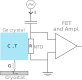
\includegraphics[width=0.3\textwidth]{graphics/bolo_simple.pdf}
\caption{\label{bolo-model} \em Simplified scheme of a RED bolometer coupling a thermal system (left side) and an electrical system (right side). }
\end{figure}

Here are some hints and info to help you understand the behavior of the bolometers (calculation and discussion in parallel with the measurements):
\begin{itemize}
	\item The heat power injected by the cryostat into the bolometer is $$P_{cryo} = G \left( T_{cryo} - T\right) \quad [\textrm{in } Watt]$$ In the considered simplified system, only the limiting conductance is considered (the lowest) which is generally the electron-phonon coupling (more in discussion..)
	\item A lot can be understand from studying the stationary state ($dT/dt=0$) and the time resolution (useful to introduce $\Delta T = T - T_{eq}$) of the heat equilibrium equation in the stationary state. Just recall that with $t$ the time and $U$ the energy of the thermal bath $$\frac{dU}{dt} = C \frac{dT}{dt} \quad [\textrm{in }  Joule]$$
	\item Some reference value for RED bolometers:
	$$ R = \mathcal{O}(1 \ G\Omega),\
	C \approx 3 \times 10^{-10} \ J.K^{-1},\
	G \approx 2 \times 10^{-8} \ W.K^{-1},\
	I = \mathcal{O}(1 \ nA),\
	T_{cryo} \approx 20 \ mK $$
	\item An optimized bolometer has the highest sensitivity $S_V$ in V/keV possible. Not to confuse with the sensitivity of the thermal sensor $\alpha$ which is usually introduced in this type of calculation 
	$$\alpha = \frac{1}{R} \frac{dR}{dT} $$
\end{itemize}


\subsection{Modélisation électrothermique du détecteur}

Dans cette partie, sont présenté les calculs théoriques permettant de construire le modèle du détecteur. L'étude s'est focalisée sur la résolution au premier ordre du système d'équations différentielles couplées en utilisant une méthode d'algèbre linéaire \cite{matrix}. Il est alors possible de simuler le comportement d'un détecteur dans l'état stationnaire, dans le régime temporel et dans le régime fréquentiel, ce qui donne accès à la caractérisation complète du détecteur.

\subsubsection{Description du modèle}

\begin{figure}[!ht]
%\centering
%\resizebox{0.6\textwidth}{!}{%
%\shorthandoff{:!}\begin{circuitikz}[scale=1]
%	\input{Images/thermal_scheme.tikz}
%\end{circuitikz}\shorthandon{:!}
%}%
\begin{center}
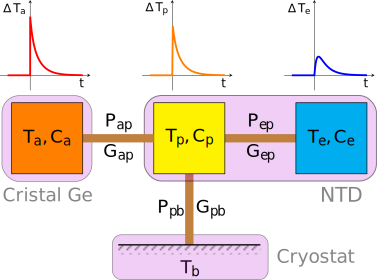
\includegraphics[width=0.6\textwidth]{Images/thermal_scheme.pdf}
\end{center}
\caption{Schéma thermique de RED1 et RED10 avec représentation de la diffusion d'un signal créée par un évènement dans le cristal de germanium. Chaque bain thermique est caractérisé par une température $T$ et une capacité thermique $C$. Chaque lien thermique est associé à une conductivité thermique $G$ et un transfert de puissance thermique $P$. Le senseur NTD est modélisé comme un système de phonons (index $p$) et un systèmes d'élécrons (index $e$) couplés thermiquement. Le bain absorbeur (index $a$) et  le cryostat (index $b$) sont tout deux reliés au bain de phonon du NTD. 
}
\label{thermal-scheme}
\end{figure}

\begin{figure}[!ht]
\begin{minipage}[c]{0.45\textwidth}
\resizebox{!}{\textwidth}{%
%\shorthandoff{:!}
\begin{circuitikz}[scale=1]
	  	\draw
	 (0.5,6) node [ground, rotate=-90] {} 
	 to [european voltage source, v=$V_B$, -*] (2,6)
	 to [european voltage source, l={\color{red} $e_{J_{RL}}$}, color=red] (2,4.5)	 
	 to [R, l_=$R_L$, -] (2,2.5)
	 to [thR, l_=$R(T_e)$, -] (2,0.5)
	 to [european voltage source, l={\color{red} $e_{J_{NTD}}$}, color=red]
	  (2,-0.5) node [ground] {}
	 (2,2.5) to [short, -o] (4,2.5) node [anchor=south] {$V$}
	 to [C, l_=$C_{fil}$] (4,-0.5) node [ground] {} 
	 (4,2.5) to [european voltage source, l={\color{red} $e_{ampli.}$}, color=red] (6,2.5) 
	 to [ioosource, l={\color{red} $i_{ampli.}$}, color=red] (6,-0.5) node [ground] {} 
	 (6,2.5) node [anchor=south] {$U$}
	 to [short, i_={\small $i \approx 0$}, *-] (7,2.5)
	 to [amp, l=Suiveur, -] (8,2.5)
	;
\end{circuitikz}
%\shorthandon{:!}
}%
\end{minipage}
\hfill
\vrule{}
\hfill
\begin{minipage}[c]{0.45\textwidth}
\begin{center}
avec Thèvenin-Norton, en fréquentiel :
\end{center}
\resizebox{\textwidth}{!}{%
%\shorthandoff{:!}
\begin{circuitikz}
		\draw
	 (0,0) node [ground] {}
	 to [R, l_=$Z_{eq}$, -] (0,2)
	 (0,2) to [short, -o] (2,2) node [anchor=south] {$V$}
	 to [ioosource, l=$\color{red} i_{noise}$,color=red, -] 
	 (2,0) node [ground] {}
	 (2,2) to [european voltage source, l={\color{red} $e_{ampli.}$}, color=red, -] (4,2) node [anchor=south] {$U$}
	 to [short, i_={\small $i \approx 0$}, *-] (5,2)
	 to [amp, l=Amplifier, -] (6,2)
	 (0,-1.5) node [right]{$\color{red} \displaystyle i_{noise}^2=\left(\frac{e_{J_{NTD}}}{R(T_e)}\right)^2+\left(\frac{e_{J_{R_L}}}{R_L}\right)^2+i_{ampli.}^2$}
	;

\end{circuitikz}
%\shorthandon{:!}
}%
\end{minipage}
\caption{Schémas de l'électronique de polarisation. La résistance NTD $R(T_e)$, la résistance de charge $R_L$ et la capacité du câblage $C_{fil}$ deviennent l'impédance complexe équivalente $Z_{eq}$. Les sources de bruits apparaissent en rouge. Les bruits Johnson, $e_{J_{RL}}$ et $e_{J_{NTD}}$, ainsi que le bruit en courant de l'amplificateur $i_{ampli.}$ sont regroupés en un bruit en courant $i_{bruit}$ dont l'expression est précisée.}
\label{electric-scheme}
\end{figure}

On utilise l'approximation d'un système de trois bains thermiques pour modéliser un détecteur RED \cite{note}. Le schéma thermique d'un détecteur dans une telle approximation est présenté dans la \hyperref[thermal-scheme]{Figure 1}. Ce modèle modélise au mieux \cite{albert} \cite{benjamin} un absorbeur en cristal de germanium sur lequel est collé un unique senseur thermique NTD. Comme présenté sur la \hyperref[thermal-scheme]{Figure 1}, il y a trois bains thermiques, chacun caractérisé par une capacité thermique $C$ et une température $T$ :
\begin{itemize}
\item en orange, le cristal de germanium jouant le rôle d'absorbeur ($T_a$, $C_a$),
\item en jaune, le bain thermique des phonons dans la résistance NTD ($T_p$, $C_p$),
\item en bleu, le bain thermique des électrons dans la résistance NTD ($T_e$, $C_e$).
\end{itemize}
Ils sont reliés par des liens thermiques caractérisés par des conductivités thermiques $G$, ce qui permet un transfert de puissance $P$ entre les bains. Il y a également la présence d'une fuite thermique de la résistance NTD vers le cryostat (en tirets noirs) ce qui permet de fixer une température de fonctionnement $T_b$.
Afin de mesurer la variation de résistance du NTD, engendrée par un dépôt d'énergie au sein du détecteur lors d'une interaction avec une particule, il est nécessaire de polariser le senseur en courant. Cela se fait en ajoutant une résistance de charge très élevée en série. Le senseur NTD est alors parcouru par un courant de polarisation $I_P$ quasiment constant pendant un évènement \cite{elec}. Le schéma électronique qui permet la polarisation et la mesure de la tension $V$ aux bornes de la résistance NTD est présenté sur la figure \ref{electric-scheme}. Il y a à gauche le schéma de l'électronique de polarisation avec représentation des bruits (en rouge) et à droite la simplification du schéma par transformation de Thèvenin-Norton \cite{mather} dans le cadre de l'étude fréquentielle, qui viendra plus tard. Une tension de polarisation constante $V_B$ est appliquée à la résistance de charge $R_L$, de quelques $G\Omega$, en série avec la résistance du NTD $R(T_e)$ dépendante de la température du bain d'électrons. On tient compte de la capacité du câblage $C_{fil}$ de l'électronique.

Afin de prédire la réponse du détecteur à un évènement, il faut maintenant résoudre ce modèle électro-thermique. On définit alors le système d'équations différentielles couplées par l'échange de puissance entre les bains thermiques, et avec le système électronique par la puissance Joule induite par le courant de polarisation au sein du senseur NTD.

Pour le système d'électrons du NTD, on a d'abord une puissance provenant de l'effet Joule $P_J= I_P^2 R(T_e)=\frac{V^2}{R(T_e)}$. On a ensuite le transfert de puissance provenant du système phonons du NTD s'exprimant comme : $P_{ep}=V_{NTD} g_{ep} (T_e^n - T_p^n)$ où $V_{NTD}$ est le volume du senseur NTD, $g_{ep}$ est la constante de couplage électron-phonon par unité de volume et $n$ est un exposant dépendant du matériau qui vaut typiquement 6 pour les thermistors tel que les NTD en germanium. L'équation d'équilibre thermique pour le bain électrons est,
\begin{equation}
\label{electron}
 C_e \frac{d T_e}{d t} = \frac{V^2}{R(T_e)} - V_S g_{ep} \left( T_e^{n} - T_p^{n} \right)
\end{equation}

Pour l'absorbeur, le bain thermique représente uniquement le système de phonons du cristal de germanium. Ce matériau étant semi-conducteur sous forme de cristal ultra-pur, il n'existe pas d'électrons libres. L'absorbeur échange une puissance  avec le système de phonons du NTD en considérant la capacité thermique de la colle comme étant négligeable. Celle-ci s'écrit $P_{ap}=g_{glue} S_{NTD} \left( T_p^{n_g} - T_a^{n_g} \right)$ avec $S_{NTD}$ la surface du NTD collé sur l'absorbeur, $g_{glue}$ la constante de conductivité thermique par unité de surface et $n_g$ un exposant. Ces deux paramètres ont été fixé expérimentalement lors d'études précédentes. L'équation d'équilibre thermique pour ce bain est donc,
\begin{equation}
\label{absorbeur}
C_a \frac{d T_a}{d t} = g_{glue} S_{NTD} \left( T_p^{n_g} - T_a^{n_g} \right)
\end{equation}


Pour le système de phonons du NTD, on a la puissance provenant du couplage phonon-électron $P_{ep}$, le transfert de puissance provenant du cristal de germanium $P_{ap}$, et la fuite thermique d'or vers le cryostat. Cette conduction thermique est assurée par deux surfaces d'or $S_{Au}$ (une sur le NTD, une sur le support) reliées par des fils d'or. On a affaire à un processus non-diffusif appelé conduction Kapitza qui s'exprime : $P_{pb}=S_{Au} g_k (T_p^{n_k} - T_b^{n_k})$ avec $g_k$ la conductance Kapitza par unité de surface et l'exposant $n_k=4$. On néglige cette fois la capacité thermique des surfaces et fils d'or, tout en considérant une capacité thermique du support en cuivre infinie, permettant de garder une température fixe $T_b$ à tout temps.
Ce bain est décrit par l'équation :
\begin{equation}
\label{phonon}
C_p \frac{d T_p}{d t} = -g_{glue} S_{NTD} \left( T_p^{n_g} - T_a^{n_g} \right)  + V_S g_{ep} \left( T_e^{n} - T_p^{n} \right) - g_k S_{Au} \left( T_p^{n_k} - T_b^{n_k} \right)
\end{equation}

Le système électrique prend en compte la variation du courant de polarisation (effet du second ordre sir $R_L\ll R_{NTD}$). L'équation associée est,
\begin{equation}
\label{polarisation}
C_{fil} \frac{d V}{d t} = \frac{V_B - V}{R_L} - \frac{V}{R(T_e)}
\end{equation}

En rassemblant les équations \ref{electron}, \ref{absorbeur}, \ref{phonon} et \ref{polarisation}, on peut composer un système d'équations différentielles couplées qui décrit complètement le modèle électro-thermique présenté dans les figures \ref{thermal-scheme} et \ref{electric-scheme}.

\begin{align}
\label{ode}
 C_a \frac{d T_a}{d t} &= g_{glue} S_{NTD} \left( T_p^{n_g} - T_a^{n_g} \right) \nonumber \\ 
 C_p \frac{d T_p}{d t} &= -g_{glue} S_{NTD} \left( T_p^{n_g} - T_a^{n_g} \right)  + V_S g_{ep} \left( T_e^{n} - T_p^{n} \right) - g_k S_{Au} \left( T_p^{n_k} - T_b^{n_k} \right) \nonumber \\ 
 C_e \frac{d T_e}{d t} &= \frac{V^2}{R(T_e)} - V_S g_{ep} \left( T_e^{n} - T_p^{n} \right) \nonumber \\ 
 C_{fil} \frac{d V}{d t} &= \frac{V_B - V}{R_L} - \frac{V}{R(T_e)}
\end{align}

\subsubsection{Solution de l'état stationnaire}
\label{steady-section}

L'étude de l'état stationnaire permet d'obtenir les grandeurs physiques autour desquels les perturbations du système vont se produire. Il est essentiel de le calculer pour obtenir les valeurs de résistance NTD, des capacités thermiques et des conductivité thermiques. Il est également nécessaire pour effectuer une opération de linéarisation par la suite. L'état stationnaire est expérimentalement défini par la température du cryostat $T_b$ et le courant de polarisation $I_P$. 

Il suffit d'annuler les termes de dérivées temporelles dans le système d'équations (\ref{ode}) pour obtenir le système d'équations dans l'état stationnaire avec ($\bar{T}_a, \bar{T}_p, \bar{T}_e, \bar{V}$) étant les solutions de l'état stationnaire :
\begin{align}
\label{steady}
0 &= g_{glue} S_{NTD} \left( \bar{T}_p^{n_g} - \bar{T}_a^{n_g} \right) \nonumber \\
0 &= -g_{glue} S_{NTD} \left( \bar{T}_p^{n_g} - \bar{T}_a^{n_g} \right) + V_S  g_{ep} \left( \bar{T}_e^{n} - \bar{T}_p^{n} \right) - g_k S_{Au} \left( \bar{T}_p^{n_k} - \bar{T}_b^{n_k} \right) \nonumber \\
0 &= \frac{V^2}{R(\bar{T}_e)} - V_S g_{ep} \left( \bar{T}_e^{n} - \bar{T}_p^{n} \right) \nonumber \\
0 &= \frac{V_B - V}{R_L} - \frac{V}{R(\bar{T}_e)}
\end{align}

Les équations sont non linéaires de part l'expression des puissances échangées et de la résistance NTD. Il est nécessaire d'employer une résolution numérique pour résoudre ce système. 


\subsubsection{Comportement dans le domaine temporel}
\label{temporal}


La résolution du système d'équations (\ref{ode}) donnerait les expressions exactes de l'évolution temporelle des températures des différents bains $T_a(t), T_p(t), T_e(t)$ et de la tension aux bornes du NTD $V(t)$. Toutefois, la très forte non-linéarité du système ne permet pas une résolution analytique. Néanmoins, seule la réponse du système à un évènement nous intéresse. L'énergie déposée d'environ $1$keV par une particule dans l'absorbeur s'exprime comme une élévation de température de l'ordre de $100~\mu K$, ce qui donne une variation de tension aux bornes du NTD de l'ordre de $100~nV$. Il est ainsi question d'étudier la réponse du système à de très faibles signaux. On se propose d'appliquer une théorie perturbative au premier ordre au système d'équations (\ref{ode}). Avec la linéarisation des termes, il est possible de définir des conductivités thermiques pour les différents liens :
\begin{itemize}
\item colle cristal-NTD : \begin{equation}\label{g1} G_{ap}^a  = n_g g_{glue} S_{NTD} \bar{T}_a^{n_g-1} \qquad \textrm{et} \qquad G_{ap}^p  = n_g g_{glue} S_{NTD} \bar{T}_p^{n_g-1}
\end{equation}
\item couplage électrons-phonons : \begin{equation}\label{g2} G_{ep}^e  = n g_{ep} V_S \bar{T}_e^{n-1} \qquad \textrm{et} \qquad G_{ep}^p  = n g_{ep} V_S \bar{T}_p^{n-1}
\end{equation}
\item fuite thermique avec fils d'or : \begin{equation}\label{g3} G_{pb} = n_k g_{k} S_{Au} \bar{T}_p^{n_k-1}
\end{equation}
\end{itemize}
On remarquera que les conductivités ont un "sens" d'utilisation comme elles dépendent de la température des bains. En retranchant (\ref{ode}), on obtient alors un système d'équations linéaires couplées :
\begin{align}
\label{tempo}
C_a \frac{d \Delta T_a}{d t}
	&= -G_{ap}^a \Delta T_a + G_{ap}^p \Delta T_p 
	\nonumber \\
C_p \frac{d \Delta T_p}{d t} 
	&= +G_{ap}^a \Delta T_a - G_{ap}^p \Delta T_p
	+ G_{ep}^e \Delta T_e - G_{ep}^p \Delta T_p
	- G_{pb}^p \Delta T_p
	\nonumber \\
C_e \frac{d \Delta T_e}{d t}
	&= - G_{ep}^e \Delta T_e + G_{ep}^p \Delta T_p
	+2\frac{\bar{V}}{R(\bar{T}_e)} \Delta V - \frac{\bar{V}^2}{R(\bar{T}_e)^2} \left.\frac{d R}{d T}\right\vert_{T_e} \Delta T_e
 	\nonumber \\
C_{fil} \frac{d \Delta V}{d t} &= - \left( \frac{1}{R_L} + \frac{1}{R(\bar{T}_e)} \right) \Delta V + \frac{\bar{V}}{R(\bar{T}_e)^2} \left.\frac{d R}{d T}\right\vert_{\bar{T}_e} \Delta T_e
\end{align}
Celui-ci peut se simplifier :
\begin{align}
\label{tempo-bis}
\frac{d \Delta T_a}{d t}
	&= -\frac{G_{ap}^a}{C_a} \Delta T_a + \frac{G_{ap}^p}{C_a} \Delta T_p 
	\nonumber \\
\frac{d \Delta T_p}{d t} 
	&= \frac{G_{ap}^a}{C_p} \Delta T_a - \frac{G_{ap}^p+G_{ep}^p+G_{pb}^p}{C_p} \Delta T_p	+ \frac{G_{ep}^e }{C_p}\Delta T_e
	\nonumber \\
\frac{d \Delta T_e}{d t}
	&= \frac{G_{ep}^p}{C_e} \Delta T_p - \frac{1}{C_e} \left(G_{ep}^e + \frac{\bar{V}^2}{R(\bar{T}_e)^2} \left.\frac{d R}{d T}\right\vert_{\bar{T}_e}\right) \Delta T_e 
	+2 \frac{1}{C_e} \frac{\bar{V}}{R(\bar{T}_e)} \Delta V
 	\nonumber \\
\frac{d \Delta V}{d t} &= \frac{1}{C_{fil}} \frac{\bar{V}}{R(\bar{T}_e)^2} \left.\frac{d R}{d T}\right\vert_{\bar{T}_e} \Delta T_e - \frac{1}{C_{fil}}\left( \frac{1}{R_L} + \frac{1}{R(\bar{T}_e)} \right) \Delta V 
\end{align}
On étudie désormais un système d'équations linéaires. Il est ainsi possible de les résoudre analytiquement. Pour cela, on peut réécrire ce système d'équations sous forme matricielle afin de faciliter les calculs. On introduit le vecteur $\bm{\phi}$ contenant les perturbations de températures et de la tension :
\begin{equation}
\label{phi}
\bm{\phi} = 
\left( \begin{array}{c}
\Delta T_a\\
\Delta T_p\\
\Delta T_e\\
\Delta V
\end{array} \right)
\end{equation}
Le système (\ref{tempo-bis}) devient simplement :
\begin{equation}
\label{ode-mat}
\frac{d \bm{\phi}}{d t}= - \bm{M} \bm{\phi} + \bm{F}(t-t_0)
\end{equation}
où $\bm{M}$ est la matrice regroupant les termes de couplages életro-thermiques. Elle découle directement des équations précédentes (\ref{tempo-bis}), et s'exprime :
\begin{equation}
\label{coupling-mat-temp}
\bm{M} = 
\left( \begin{array}{cccc}
 \frac{G_{ap}^a}{C_a}&-\frac{G_{ap}^p}{C_a}&0&0 \\
 -\frac{G_{ap}^a}{C_p}&\frac{G_{ap}^p+G_{ep}^p+G_{pb}^p}{C_p}&-\frac{G_{ep}^e}{C_p}&0 \\
0&-\frac{G_{ep}^p}{C_e}&\frac{1}{C_e}\left(G_{ep}^e + \frac{V^2}{R(T_e)^2}  \left.\frac{d R}{d T}\right\vert_{T_e} \right)&-2\frac{V}{R(T_e)}\\
0&0&-\frac{1}{C_{fil}}\frac{V}{R(T_e)^2} \left.\frac{d R}{d T}\right\vert_{T_e} &\frac{1}{C_{fil}}\left( \frac{1}{R_L} + \frac{1}{R(T_e)} \right)
\end{array} \right)
\end{equation}
Il a également été ajouté un terme de source $\bm{F}$ qui permet de contenir les dépôts d'énergie dans le détecteur et les différentes sources de bruits parasites. Dans le cas d'une particule déposant une énergie $E$ dans l'absorbeur, ce terme s'exprime comme,
\begin{equation}
\bm{F}(t-t_0) = 
\left( \begin{array}{c}
E/C_a \\
0 \\
0 \\
0
\end{array} \right) \delta (t-t0)
\end{equation}
On considère ici le dépôt de l'énergie de recul, la relaxation des phonons créés dans l'absorbeur, et l'élévation en température de celui-ci comme étant des processus instantanés, d'où l'utilisation de la fonction de Dirac $\delta (t-t_0)$. Une variante de ce modèle consiste à attribuer un temps de relaxation aux phonons et de prendre en compte la montée en température des bains thermiques lors de la relaxation des phonons.

La solution générale de l'équation (\ref{ode-mat}) est une combinaison linéaire de $N$ exponentielles, avec $N=4$ correspondant aux dimensions du système, chacune étant caractérisée par une constante de temps. On obtient leur expression en diagonalisant la matrice de couplage $\bm{M}$ pour se placer dans la base propre des solutions du système. On considère, pour $i=1,2,3,4$, les vecteurs propres $\bm{v}_i$ et les valeurs propres associées pour écrire ces solutions,
\begin{equation}
\label{eigen-soluc}
\bm{f}_i(t) = f_i(t) \bm{v}_i
\end{equation}
Sans considérer le terme de source, on introduit ces expressions dans l'équation matricielle (\ref{ode-mat}) pour donner
\begin{equation}
\label{eigen-soluc-ode}
\frac{d \bm{f}_i(t)}{d t} = -f_i(t) \bm{M} \bm{v}_i = -\lambda_i f_i(t) \bm{v}_i
\end{equation}
La résolution de cette équation amène à l'expression des solutions dans la base propre $f_i(t) = A_i e^{-t/\tau_i} \bm{v}_i$ avec $A_i$ la constante de normalisation et $\tau_i=1/\lambda_i$ la constante de temps de la solution. La solution générale de (\ref{ode-mat}) s'exprime alors dans la base propre comme
\begin{equation}
\label{eigein-solc-expr}
\bm{f}(t) = \sum_i A_i e^{-t/\tau_i} \bm{v}_i
\end{equation}
Pour faire le lien entre la base propre et les fluctuations de températures et de tension, il faut projeter la solution $\bm{f}$ sur les 4 vecteurs orthogonaux formant $\bm{\phi}$ tel que :
\begin{equation}
\label{gen-soluc}
\phi_j = \bm{f} \cdot \bm{\phi}_j = \sum_i^4 f_i(t) \bm{v}_i \cdot \bm{\phi}_j = \sum_i P_{ij} f_i(t) = \sum_i P_{ij} A_i e^{-t/\tau_i}
\end{equation}
où $P_{ij}$ désigne les vecteurs composant la matrice de passage satisfaisant $\bm{M}=\bm{P} \bm{D} \bm{P}^{-1}$.

Pour fixer les constantes de normalisation $A_i$, on utilise les conditions initiales du système :
\begin{equation}
\bm{\phi}(0) = \bm{F}(0) =
\left( \begin{array}{c}
\sum_i P_{ai} A_i\\
\sum_i P_{pi} A_i\\
\sum_i P_{ei} A_i\\
\sum_i P_{vi} A_i
\end{array} \right) = \bm{P} \bm{A}
\qquad \longrightarrow \qquad \bm{A}=\bm{P}^{-1} \bm{\phi} (0)
\label{normal}
\end{equation}
avec $\bm{A}$ le vecteur contenant les constantes $A_i$.

L'étude d'un détecteur en temporel revient à résoudre l'équation matricielle (\ref{ode-mat}) et donc à trouver les valeurs et vecteurs propres de la matrice de couplage $\bm{M}$. Le modèle électro-thermique est maintenant complètement décrit dans le domaine temporel.

\subsubsection{Réponse en domaine fréquentiel}
\label{omega}

L'étude des bruits menant au calcul de la résolution du détecteur nécessite de décrire maintenant le comportement en régime fréquentiel. En effet, les bruits d'un système sont bien caractérisés d'un point de vue fréquentiel : on peut avoir accès à l'expression de leur densité spectrale.
On considère la transformée de Fourier de l'équation matricielle (\ref{ode-mat}),
\begin{equation}
\bm{C} (i\omega + \bm{M})  \bm{\tilde{\phi}}  (\omega) = \bm{Z} (\omega) \bm{\tilde{\phi}} (\omega)  = \bm{C} \bm{\tilde{F}} (\omega) \qquad \textrm{avec} \qquad \bm{C} = \left( \begin{array}{cccc}
 C_a&0&0&0 \\
0&C_p&0&0\\
0&0&C_e&0\\
0&0&0&C_{fil}
\end{array} \right)
\end{equation}
où l'on introduit une matrice $\bm{Z}$ contenant les couplages électro-thermiques exprimés dans le régime fréquentiel. En explicitant cette équation :
\begin{equation}
\label{z-mat}
\bm{Z} (\omega) \bm{\tilde{\phi}} (\omega) =
\left( \begin{array}{cccc}
 \frac{1}{a}&-g&0&0 \\
-b&\frac{1}{c}&-h&0\\
0&-d&\frac{1}{e}-k&-l\\
0&0&-f&Z_{eq}^{-1}
\end{array} \right)
\left( \begin{array}{c}
\Delta T_a\\
\Delta T_p\\
\Delta T_e\\
\Delta V
\end{array} \right)
 =
\left( \begin{array}{c}
W\begingroup\color{red} - P_{ap}\endgroup\\
\begingroup\color{red}  P_{ap} + P_{ep} + P_{bp}\endgroup\\
\begingroup\color{red} - P_{ep}\endgroup\\
\begingroup\color{red}  i_{bruit} \endgroup
\end{array} \right)
=  \bm{C} \bm{\tilde{F}} (\omega)
\end{equation}
avec les termes rouges étant des bruits en puissance et en courant introduits dans le diagramme en blocs \ref{block-diagram}. Les coefficients de la matrice $\bm{Z}$ découlent du système d'équations linéarisées (\ref{ode}) tels que :
\begin{equation}
\begin{aligned}[c]
a &=(i C_a \omega + G_{ap}^a)^{-1} \\
b &=G_{ap}^a \\
c &=(i C_p \omega + G_{ap}^p + G_{ep}^p + G_{pb})^{-1} \\
d &=G_{ep}^p \\
e &=(i C_e \omega + G_{ep}^e)^{-1}\\
f &=\frac{(dR/dT) V}{R^2} 
\end{aligned}
\qquad \qquad
\begin{aligned}[c]
g &=G_{ap}^p \\
h &=G_{ep}^e \\
k &=- \frac{(dR/dT) V^{2}}{R^{2}} \\
\ell &=\frac{2 V}{R}
\end{aligned}
\label{coef}
\end{equation}
et avec l'impédance complexe $Z_{eq}$ contenant les composants électriques du circuit de polarisation conformément à la figure (\ref{electric-scheme}) :
\begin{equation}
Z_{eq} = \left(\frac{1}{R_L} + \frac{1}{R(T_e)} + i\omega C_{fil}\right)^{-1}
\end{equation}
L'expression du vecteurs des fluctuations $\bm{\phi}$ s'obtient en inversant la matrice couplage $\bm{Z}$ comme, 
\begin{equation}
\bm{\tilde{\phi}} (\omega) =
\left( \begin{array}{c}
\Delta \tilde{T}_a\\
\Delta \tilde{T}_p\\
\Delta \tilde{T}_e\\
\Delta \tilde{V}
\end{array} \right)
=
\left( \begin{array}{cccc}
 Z_{aa}^{-1}&Z_{ap}^{-1}&Z_{ae}^{-1}&Z_{av}^{-1} \\
 Z_{pa}^{-1}&Z_{pp}^{-1}&Z_{pe}^{-1}&Z_{pv}^{-1}\\
 Z_{ea}^{-1}&Z_{ep}^{-1}&Z_{ee}^{-1}&Z_{ev}^{-1}\\
 Z_{va}^{-1}&Z_{vp}^{-1}&Z_{ve}^{-1}&Z_{vv}^{-1}
\end{array} \right)
\left( \begin{array}{c}
\Delta \tilde{P}_a\\
\Delta \tilde{P}_p\\
\Delta \tilde{P}_e\\
\Delta \tilde{I}
\end{array} \right)
= \bm{Z}^{-1}(\omega) \bm{\tilde{F}} (\omega)
\end{equation}
On remarque ici que le formalisme matriciel associé à un outil de calcul numérique permet d'avoir facilement accès aux perturbations de températures et de tension à partir de la matrice de couplage et des sources de puissances externes contenues dans le vecteur $\bm{\tilde{F}}(w)$.

\begin{figure}[!ht]
\begin{center}
\resizebox{\textwidth}{!}{%
\begin{tikzpicture}
	    \sbEntree{W}
    \sbCompSum{C1}{W}{-}{+}{+}{}
    	\sbRelier{W}{C1}
        \sbNomLien[0.8]{W}{$W$}
    \sbBloc{a}{$a$}{C1}
        \sbRelier{C1}{a}
    \sbBloc[3]{b}{$b$}{a}
        \sbRelier[$\Delta T_a$]{a}{b}  
    \sbCompSum{C2}{b}{+}{+}{+}{}
        \sbRelier{b}{C2}      
    \sbBlocL{c}{$c$}{C2}
    \sbBloc[3]{d}{$d$}{c}
    	\sbRelier[$\Delta T_p$]{c}{d}
    \sbCompSum{C3}{d}{-}{+}{+}{}
    	\sbRelier{d}{C3}		
    \sbBlocL{e}{$e$}{C3}	      
    \sbBloc[3]{f}{$f$}{e}
    	\sbRelier[$\Delta T_e$]{e}{f}
    \sbCompSum{C4}{f}{+}{}{+}{}
        \sbRelier{f}{C4}
    \sbBlocL{Z}{$Z_{eq}$}{C4}
    \sbCompSum[5]{C5}{Z}{+}{}{+}{}
        \sbRelier[$\Delta U$]{Z}{C5}
    \sbSortie{V}{C5}
        \sbRelier{C5}{V}
        \sbNomLien[0.8]{V}{$\Delta V$}
    
    \sbDecaleNoeudy[5]{a-b}{down1}
	\sbBlocr{g}{$g$}{down1}
		\sbRelieryx{c-d}{g}
    	\sbRelierxy{g}{C1}
    \sbDecaleNoeudy[8]{c-d}{down2}
	\sbBlocr{h}{$h$}{down2}
		\sbRelieryx{e-f}{h}
    	\sbRelierxy{h}{C2}
	\sbDecaleNoeudy[10]{d}{down5}
	\sbCompSum{C6}{down5}{}{+}{}{+}
	\sbBloc{k}{$k$}{C6}
	\sbDecaleNoeudy[13]{C4-Z}{down4}
	\sbBlocr{l}{$\ell$}{down4}
		\sbRelier[$\Delta P_J$]{C6}{C3}
		\sbRelieryx{e-f}{k}
    	\sbRelier{k}{C6}	
		\sbRelieryx{Z-C5}{l}
    	\sbRelierxy{l}{C6}
    
    \sbStyleLien{red,text=red}
    \sbDecaleNoeudy[-4]{C1}{Pap}
    	\sbRelier{Pap}{C1}
    	\sbNomLienCustom[0.3]{Pap}{$P_{ap}$}
    \sbDecaleNoeudy[-4]{C2}{sumP}
    	\sbRelier{sumP}{C2}
    	\sbNomLienCustom[0.3]{sumP}{$P_{ap}+P_{ep}+P_{bp}$}
    \sbDecaleNoeudy[-4]{C3}{Pep}
    	\sbRelier{Pep}{C3}
    	\sbNomLienCustom[0.3]{Pep}{$P_{ep}$}
    \sbDecaleNoeudy[-4]{C4}{i}
    	\sbRelier{i}{C4}
    	\sbNomLienCustom[0.3]{i}{$i_{bruit}$}  
    \sbDecaleNoeudy[-3]{C5}{eA}
    	\sbRelier{eA}{C5}
    	\sbNomLienCustom[0.3]{eA}{$e_{ampli.}$}   
\end{tikzpicture}
}%
\end{center}
\caption{Diagramme en bloc du modèle électro-thermique avec injection de la puissance d'un évènement $W$, de bruits en puissance $P_{ap}, P_{ep}, P_{pb}$, d'un bruit en courant $i_{bruit}$ et d'un bruit en tension $e_{ampli.}$. Les coefficients des blocs sont précisés dans (\ref{coef}). Le formalisme des diagrammes en blocs et le formalisme matricielle sont équivalents et aboutissent à des expressions identiques pour les calculs de sensibilité et de bruit.}
\label{block-diagram}
\end{figure}

Malgré cette simplification des calculs, la compréhension des couplages entre les grandeurs observées n'est pas très aisée. Une meilleure compréhension est possible en convertissant le système d'équations (\ref{ode-mat}) dans un formalisme de diagramme en blocs \cite{block-diagram} présenté à la figure \ref{block-diagram}. On y retrouve les coefficients de couplages utilisés dans la matrice de couplage $\bm{Z}$ ainsi que les sources de puissances externes. On peut visualiser plus aisément le couplage entre les différents bains ainsi que la diffusion de la puissance déposée par une particule dans l'absorbeur $W$.

La réponse du système à un évènement est caractérisée par la sensibilité $s_V$. Dans le cas d'une interaction de particule déposant toute l'énergie de recul dans l'absorbeur, la sensibilité s'exprime ${s}_V(\omega) = Z_{va}^{-1}\hat{p}(\omega)$ avec $\hat{p}(\omega)$ la transformée de Fourier du signal en puissance $W$. L'approximation d'un dépôt d'énergie de recul instantané donne $\hat{p}(\omega) = \hat{\delta} = 1$, ce qui simplifie énormément les calculs. La variante où l'on considère le temps de relaxation des phonons nécessite de multiplier par la fonction passe-bas $\hat{p}(\omega) = 1/(1+i\omega \tau_P)$ avec $\tau_P$ la constante de temps correspondant au temps de relaxation des phonons au sein du détecteur. D'autres expériences de détection directe, telles que CDMS \cite{julien}, travaillent par la détection des phonons athermaux qui traverseraient les différentes parties du détecteur avant de se relaxer. Ainsi, il est possible d'avoir une fraction $\epsilon$ des phonons, produit lors d'un évènement, qui passe dans la résistance NTD et s'y relaxent. On observerait alors une élévation de température directement dans le senseur NTD, en plus de celle dans l'absorbeur. En prenant en compte cette possiblité, la sensibilité du système se réécrit :
\begin{equation}
\label{sv}
\hat{s}_V(\omega) = \left[(1-\epsilon) Z_{va}^{-1} + \epsilon Z_{ve}^{-1}\right]\hat{p}(\omega) \qquad [V/W]
\end{equation}
La fraction $\epsilon$ de phonons dits "athermiques" dépend très fortement de la géométrie du cristal de germanium, de son polissage, de la colle utilisée entre l'absorbeur et le NTD, et sûrement d'autres paramètres de l'expérience qui ne sont pas encore cernés. On détecte la présence de phonons athermiques grâce à la forme du signal : la montée en température du NTD est plus rapide et il apparait une contribution exponentielle caractérisée par la constante de temps $\tau_P$. On verra dans les parties suivantes que le détecteur RED10 présente une fraction importante de phonons athermiques qui est estimée par la forme du signal.

La résolution du diagramme en bloc \ref{block-diagram} permet de s'assurer que la boucle de rétro-action associée à la puissance Joule $\Delta P_J$ est négative, ce qui permet la stabilité de la polarisation de la résistance NTD. En effet, l'élévation en température créée par le courant de polarisation dans le NTD diminue la résistance de celui-ci conformément à la formule (\ref{ntd}), ce qui réduit en retour l'effet Joule suivi la formule $P_J=RI^2$ avec le courant de polarisation maintenu constant. Cette rétroaction négative provient de la technologie de senseur thermique utilisée : la résistance des NTD diminue avec la température. Une autre technologie de senseur thermique appelé TES \cite{julien} \cite{matrix} présente une résistance croissante avec la température. Pour obtenir une rétroaction négative et avoir une stabilité de polarisation, ces expériences utilisent une polarisation en tension et non en courant. En effet, on se place dans le cas $P_J=V^2/R$ avec $V$ maintenu constant.

Un autre avantage de cette rétroaction négative est l'atténuation des perturbations : on peut alors diminuer l'impact des bruits en général, mais en particulier des bruits thermiques \cite{mather}. Ces derniers se présentent comme la limite intrinsèque du bruit parasitant la mesure. De manière général, le seul moyen de les diminuer est d'abaisser davantage la température du cryostat, ce qui est difficile car on se heurte alors à la limite de technologie cryogénique.

Il est maintenant possible d'accéder à la densité spectrale de bruit référée à la tension aux bornes du NTD en sommant quadratiquement les différentes sources de bruits, considérant qu'elles ne sont pas corrélées entre elles. La densité spectrale en puissance de bruit totale s'exprime comme,
\begin{equation}
\label{psd-total}
S_{V,total} = \sum_i^{sources} \left\vert \sum_j^{a,p,e,v} Z_{v,j}^{-1} (\omega) \tilde{F}_j(\omega) \right\vert^2 \qquad [V^2/Hz]
\end{equation}
où la sommation quadratique s'effectue sur toutes le sources de bruits, et l'index $v$ fait référence aux coefficients de la matrice de couplage inversée relatifs à la tension aux bornes du NTD.

Les différentes sources de bruits ainsi que le niveau auquel elles interviennent sont indiqués en rouge sur la figure \ref{block-diagram}. On a tout d'abord la présence des bruits de fluctuations thermiques (TFN : Thermal Fluctuation Noise) présent pour chaque lien thermique au sein du système : $P_{ap}, P_{pb}, P_{ep}$. La PSD de ces fluctuations de puissance dans le lien reliant un bain de température $T_i$ et un bain à $T_j$ s'exprime \cite{alex} \cite{ashcroft}:
\begin{equation}
S_{P,ij} = 2k_B(T_i^2 + T_j^2) G_ij \qquad [W^2/Hz]
\end{equation}
avec la conductivité thermique du lien $G_{ij}$. Grâce à la théorie perturbative, on a obtenu des expressions de conductivités (\ref{g1},\ref{g2},\ref{g3})  dépendant du sens de transfert considéré. Le comportement du bruit TFN avec de telles conductivités n'étant pas proprement défini, on approxime une conductivité thermique effective pour le bruit TFN comme la moyenne de ces deux conductivités relatives au lien thermique. Comme le bruit TFN est associé à un lien thermique, il affecte deux bains thermiques. Il faut alors prendre en compte l'anticorrelation des contributions d'un bruit TFN dans les deux bains afin de respecter le principe de conservation de l'énergie. En adaptant l'équation (\ref{psd-total}), on peut obtenir une PSD intermédiaire regroupant tous les les termes de bruits TFN :
\begin{multline}
S_{V,TFN} = 2k_B \times  \left[ (T_a^2 + T_p^2) G_{ap} \left\vert Z_{vp}^{-1} - Z_{va}^{-1} \right\vert^2 \right. \\ \left. + (T_e^2 + T_p^2) G_{ep} \left\vert Z_{vp}^{-1} - Z_{ve}^{-1} \right\vert^2 + (T_p^2 + T_b^2) G_{pb} \left\vert Z_{vp}^{-1}\right\vert^2 \right] \qquad [V^2/Hz]
\end{multline}
En suivant les bruits indiqués sur la schéma bloc \ref{block-diagram}, on a maintenant l'intervention d'un bruit en courant $i_{bruit}$ qui provient de la transformation Thèvenin-Norton du cicuit électrique présenté sur la figure \ref{electric-scheme}. Il correspond à la somme quadratique des bruits Johnson $e_{J_{R_L}}, e_{J_{NTD}}$ liés aux résistances de charge et NTD et du bruit en courant introduit par l'électronique d'amplification $i_{ampli.}$ qui s'exprime: 
\begin{equation}
\label{i-bruit}
i_{bruit}^2 = i_{ampli}^2 + \left( \frac{e_{J_{R_L}}}{R_L} \right)^2 + \left( \frac{e_{J_{NTD}}}{R(T_e)} \right)^2 \qquad [A^2/Hz]
\end{equation}
Une résistance électrique de valeur $R$ à la température $T$ voit sa tension à ses bornes fluctuer aléatoirement de part le bruit Johnson dont la PSD est exprimée :
\begin{equation}
e_{J_R}^2 = 4k_B T R \qquad [V^2/Hz]
\end{equation}
On a ainsi la contribution des bruits Johnson à la PSD de bruit totale :
\begin{equation}
S_{V,R(T_e)} = \frac{4 k_B T_e R(T_e)}{R(T_e)^2} \left\vert Z_{vv}^{-1}\right\vert^2
\qquad \textrm{et} \qquad
S_{V,R_L} = \frac{4 k_B T_{R_L} R_L}{R_L^2} \left\vert Z_{vv}^{-1}\right\vert^2
\end{equation}
La contribution des bruits Johnson est pondérée par la résistance correspondante, il s'agit au final d'un diviseur de tension. Ainsi, les fluctuations de tension aux bornes de la résistance de charge $R_L$ sont 2 à 3 ordres supérieurs aux fluctuation de tensions aux bornes du senseur NTD $R(T_e)$ mais la pondération permet d'être prédominé par le bruit Johnson de la résistance NTD.
Les deux derniers termes de bruits en courant $i_{ampli}$ et $e_{ampli}$ proviennent de l'électronique d'amplification simplement représentée par un amplificateur suiveur sur la figure \ref{electric-scheme}. Ils sont dépendant du type d'électronique utilisée et doivent être déterminés expérimentalement. Leurs contributions à la PSD totale s'exprime :
\begin{equation}
\label{bruit-ampli}
S_{V,i_{ampli.}} = i_{ampli.}^2 \left\vert Z_{vv}^{-1}\right\vert^2 \quad [A/Hz]
\qquad
\textrm{et}
\qquad
S_{V,e_{ampli.}} = e_{ampli.}^2 \quad [V/Hz]
\end{equation}
En effet, il n'y a pas de fuite de courant vers l'électronique d'amplification, ainsi le terme de bruit en tension de l'amplificateur $e_{ampli.}$ affecte la mesure indépendamment du circuit en amont.

Maintenant que nous avons exprimé la densité spectrale de bruit sur la tension mesurée et la sensibilité du système au signal, il est possible de réaliser le calcul de la résolution du détecteur. On introduit pour cela la puissance de bruit équivalent notée NEP (Noise Equivalent Power). Cette grandeur correspond à la PSD de bruit produit dans l'absorbeur (et le système électron, si les phonons athermiques sont considérés) permettant d'induire un bruit en tension identique aux bruit totale déjà calculé par la formule \ref{psd-total}. De manière plus simple, c'est un "outil" permettant de comparer la sensibilité du système et la densité spectrale de bruit affectant la mesure, indépendamment des sources de signal et de bruits. On définit la NEP comme,
\begin{equation}
\label{nep}
NEP^2(\omega) =  \frac{S_{V,total}}{|\hat{s}_V|^2} \qquad [W^2/Hz]
\end{equation}
La NEP fait apparaître un rapport bruit sur signal, en prenant en compte la bande passante du système. On peut donc s'attendre à ce que la résolution en énergie du détecteur soir reliée à cette valeur. Des calculs décrit dans \cite{cpd}, donne alors l'expression de la résolution en énergie en fonction de la NEP:
\begin{equation}
\label{resolution}
\displaystyle{ \sigma_E^2 = \left( \int_{0}^{\infty} \frac{\mathrm{d}\omega}{2\pi}\frac{4}{|NEP(\omega)|^2}\right)^{-1} } \qquad [J^2]
\end{equation}
Les bornes d'intégration s'étendent de $0$ à l'infini seulement théoriquement. Expérimentalement, ces bornes d'intégration sont limitées par la durée de la mesure, qui fixe la borne inférieure, et la fréquence de Nyquist, qui fixe la borne supérieure. La résolution est homogène à une énergie et s'exprime en Joule. Il est d'usage de raisonner en eV et donc de multiplier la résolution par la facteur de conversion $u=(1.602\times 10^{-19})^{-1}  = 6.241 \times 10^{18} \textrm{eV/J}$.

\section{Prise de données expérimentales avec analyse par le modèle électro-thermique}

On a mis en place dans la partie précédente une modélisation des détecteurs RED. On applique maintenant ce modèle au choix de l'électronique de polarisation qui sera utilisée dans le futur, ainsi qu'à la caractérisation du nouveau détecteur RED10. Il sera ainsi possible de comparer le modèle construit aux données expérimentales issues d'acquisitions des détecteurs RED1 et RED10.

\subsection{Caractérisation de l'électronique}
\label{caract}
On a construit dans la partie précédente le modèle électro-thermique du détecteur ainsi que les outils pour étudier et simuler son comportement dans l'état stationnaire, le régime temporel, et le régime fréquentielle. Ce dernier donne accès au calcul de la résolution à partir de la sensibilité et des densités spectrales de bruits. Parmi les sources de bruits du système se sont dégagés les bruits provenant de l'électronique d'amplification (\ref{bruit-ampli}) en courant et en tension. En effet, il s'agit du bruit résultant de tous les composants contenus dans le montage d'amplification, et il n'existe pas d'expressions théorique associée. Cette partie se focalise sur la caractérisation de deux électroniques d'amplification à la disposition du laboratoire. Il sera ainsi possible d'évaluer la PSD totale de bruit et d'obtenir des valeurs numériques pour la résolution.

Les deux électroniques à disposition seront appelées CUORE et EDELWEISS, en référence à leur expérience de provenance. Ces deux électroniques reposent sur l'action d'un transistor à effet de champ désigné FET (Field Effect Transistor). La différence majeure entre CUORE et EDELWEISS provient de la différence de FET utilisé. Dans le cas de CUORE, la température de fonctionnement du FET correspond à la température ambiante. Pour EDELWEISS, le FET nécessite d'être placé dans le cryostat pour atteindre sa température de fonctionnement optimal de $150$ K. De plus, une capacité de $10$nF prend place de la résistance de charge dans le circuit. Ce composant était déjà présent de part la précédente utilisation de l'électronique EDELWEISS et n'ajoute pas de bruit supplémentaire. Seule la capacité du câblage d'EDELWEISS s'en retrouvera changée, ce qui n'entrave pas la caractérisation et la comparaison des deux électroniques.

\subsubsection{Étude du bruit}

Bien qu'il n'existe pas d'expressions précises pour les PSD des bruits en courant et tension, plusieurs modèles ont déjà été proposé pour décrire différentes technologies de transistor \cite{low-noise-electronic} \cite{alex}. À partir des mesures de PSD et la littérature, on propose le modèle de bruit suivant :
\begin{equation}
\label{i-ampli}
i_{ampli.}^2 = i_A^2 + (i_B \sqrt{f})^2 + (i_C f)^2 \qquad [A^2/Hz]
\end{equation}
\begin{equation}
\label{e-ampli}
e_{ampli.}^2 = e_A^2 + e_{BF}^2 = e_A^2 + \left( \frac{e_B}{\sqrt{f}} \right)^2 +\left( \frac{e_C}{f} \right)^2 \qquad [V^2/Hz]
\end{equation}
avec $i_{A,B,C}$ et $e_{A,B,C}$ des coefficients dont l'unité permet l'homogénéité des formules. Le terme $e_{BF}$ est relatif au bruit prédominant à basse fréquence.

L'objectif est d'ajuster au mieux le modèle proposé à des mesures des PSD expérimentales afin d'obtenir des contraintes sur les coefficients des formules (\ref{i-ampli}, \ref{e-ampli}). En plus de ces coefficients, on va aussi vouloir contraindre la capacité du câblage. On a ainsi un jeu de paramètres libres noté,
\begin{equation}
\Theta=(C_{fil}, i_A, i_B, i_C, e_A, e_B, e_C)
\end{equation}

On veut mettre en place une analyse par fonction de vraisemblance pour ajuster le modèle aux données expérimentales. Cela nécessite de connaître la distribution du bruit. Il est nécessaire pour cela de faire une mesure du bruit du système. Pour cela, on ne polarise pas la résistance NTD ($I_P=0$A), et on retire du circuit présenté à la figure \ref{electric-scheme} la résistance de charge pour ne pas être prédominé par son bruit Johnson. On choisit de travailler avec des fenêtres temporelles de $1$s avec une fréquence d'échantillonnage de $10$kHz. On applique sur ces fenêtres une méthode de Welch permettant d'estimer la densité spectrale de bruit. Des acquisitions de $120$s permettent de réaliser une moyenne des PSD de bruit mesurées.

\begin{figure}[!ht]
\begin{center}
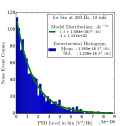
\includegraphics[width=0.6\textwidth]{Images/fit_exp_fin.pdf}
\end{center}
\caption{Histogramme de la densité spectrale de bruit à $200$ Hz ajustée par un modèle exponentiel.}
\label{noise-form}
\end{figure}

Dans un premier temps, on trace l'histogramme de la valeurs de la PSD mesurée pour différentes fréquences. Un tel histogramme est présenté pour une fréquence de $200$Hz sur la figure \ref{noise-form}. Quelque soit la fréquence sondée, la température du cryostat, ou l'électronique utilisée, on observe une forme de distribution analogue. On ajuste avec succès à ces histogrammes une distribution exponentielle. On peut appliquer au bruit une propriété de la loi exponentielle : la valeur moyenne $\mathcal{D}_i$ d'une mesure à la fréquence $i$ est égale à son écart-type $\sigma_{\mathcal{D}_i}$. En effet, les valeurs expérimentales de la moyenne et de l'écart-type sont proches du terme $1/\lambda$.
Ainsi, sur une mesure moyennée sur $N=120$ fenêtres de $1$ seconde, le Théorème Centrale Limite exprime l'écrat-type sur la mesure moyennée $\sigma_{\bar{\mathcal{D}}_i}$ tel que:
\begin{equation}
\label{sigma}
\sigma_{\bar{\mathcal{D}_i}} = \frac{\sigma_{\mathcal{D}_i}}{\sqrt{N}} = \frac{\bar{\mathcal{D}_i}}{\sqrt{120}}
\end{equation}

Cette information sur la PSD du bruit permet de construire rigoureusement une fonction de vraisemblance basée sur la fonction de $\chi^2$ relative au modèle de bruit avec les paramètres $\Theta$ et aux données expérimentales $\mathcal{D}$. Elle s'écrit :
\begin{equation}
\label{chi2}
\chi ^2 (\Theta|\mathcal{D}) = \sum^{N_{Temp}}_{j} \sum^{N_{bin}}_{i} \left[ \frac{\bar{\mathcal{D}_{ij}} - \mathcal{M}(f_{ij}; \Theta)}{\sigma_{\bar{\mathcal{D}_{ij}}}} \right]^2
\end{equation}
où on somme sur l'ensemble des fréquences $N_{bin}$ et sur l'ensemble des températures de mesure $N_{Temp}$. En effet, on ajuste simultanément le modèle sur plusieurs mesures de PSD effectuées pour des températures allant de $18$mK à $40$mK. On espère ainsi obtenir de meilleures contraintes sur les paramètres, d'abord parce qu'on analyse plus de points, mais surtout car le changement de température modifie des paramètres du système (en particulier la résistance du NTD $R(T_e)$) et permet de lever les problèmes de dégénérescence entre les différents paramètres libres.

Motivée par une approche bayésienne \cite{julien}, la fonction de vraisemblance s'exprime comme,
\begin{equation}
\label{likelihood}
\mathcal{L}(\Theta | \mathcal{D}) = \exp{\left(\frac{-\chi ^2 (\Theta|\mathcal{D})}{2}\right)}
\end{equation}


\subsubsection{Analyse par méthode de Monte Carlo avec Chaîne de Markov (MCMC)}


On recherche l'ensemble de paramètre $\Theta$ qui minimise la fonction de vraisemblance $\mathcal{L}(\Theta | \mathcal{D})$. On applique pour cela une analyse de Monte Carlo par Chaîne de Markov désignée comme méthode MCMC. Il s'agit d'une méthode reposant sur la marche aléatoire avec condition d'une (ou plus) chaine de Markov, un ensemble contenant les paramètres libres, dans l'espace de dimensions $N=7$ correspondant au nombre de paramètres libres. Il a été démontré \cite{julien} qu'avec une fonction de vraisemblance juste, la chaîne de Markov permet d'échantillonner cette fonction dans un voisinage de la solution optimale . Les avantages de la méthode MCMC sont qu'elle peut sonder une grande partie de l'espace des paramètres libres mais qu'elle converge rapidement vers le voisinage de solution optimale qu'il est alors possible d'explorer et d'analyser avec les histogrammes des positions des chaînes de Markov. La figure (\ref{triangle-mcmc}) présente de telles histogrammes pour l'électronique d'EDELWEISS.
\begin{figure}
\includegraphics[width=\textwidth]{Images/triangle_fin.pdf}
\caption{Histogramme des positions des chaînes de Markov avec projections sur 2 dimensions, lors de l'analyse MCMC pour l'électronique EDELWEISS. Les paramètres libres présentés sont de haut en bas, et de gauche à droite : $C_{fil}, i_A, i_B, i_C, e_A, e_B, e_C, e_{DAC}$.}
\label{triangle-mcmc}
\end{figure}
On extrait de l'histogramme de positions la position moyenne comme estimation de l'ensemble de paramètres libres optimaux ainsi que les barres d'erreurs à 68\% sur cette estimation à partir des 16ème et 84ème quantiles des distributions. La forme des distributions nous renseigne également sur la qualité de contrainte imposée au paramètre considéré. En effet, une distribution étroite indique un paramètre bien contraint (paramètre $i_B$) avec des faibles barres d'erreurs contrairement à une distribution étalée qui présage de grandes barres d'erreurs (paramètre $i_A$). Deux paramètres dont la projection en 2 dimensions est allongée indique leur corrélation (paramètre $i_C$ et $e_{DAC}$). 

\begin{figure}[!ht]
\begin{center}
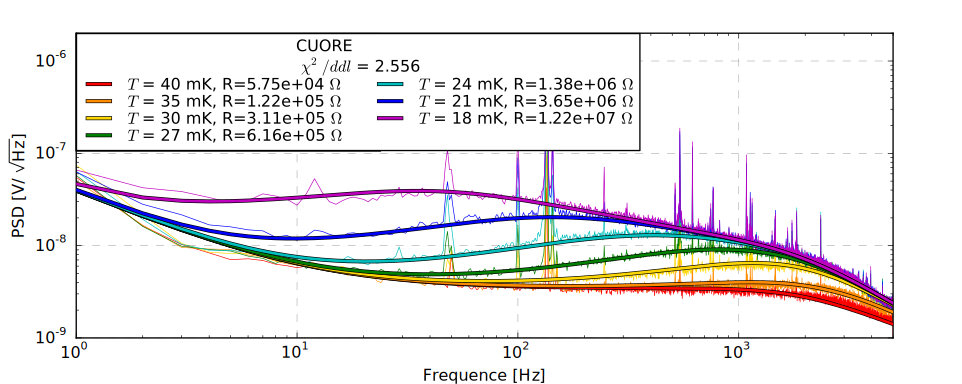
\includegraphics[width=\textwidth]{Images/cuore_fit_fin.pdf}
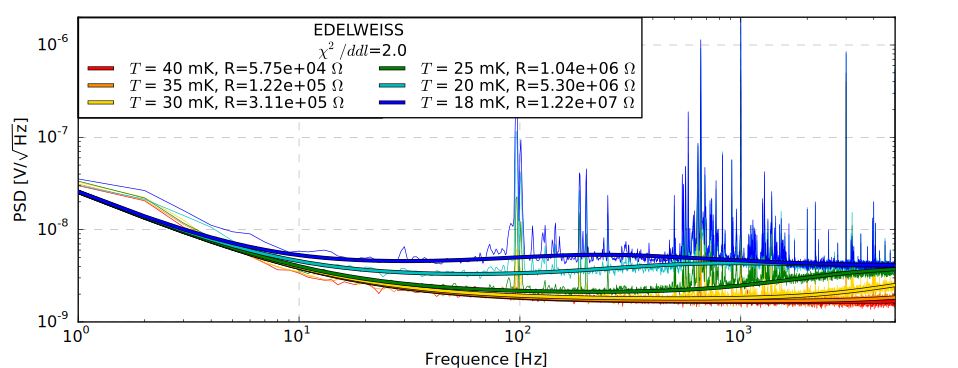
\includegraphics[width=\textwidth]{Images/edel_fit_fin.pdf}
\end{center}
\caption{Mesures moyennées (traits fins) et ajustement par analyse MCMC (traits épais) de densités spectrales de bruit pour différentes températures sur les deux électroniques : CUORE et EDELWEISS. Il est important de noter qu'il s'agit de mesures de bruit réalisées sans courant de polarisation. Pour chaque température de cryostat $T$ est précisée la valeur de la thermistance $R$. Le terme $\chi^2/ddl$ indique la valeur de la fonction $\chi^2$ divisée par le nombre de point (degrés de liberté) de l'ajustement. Pour une modélisation parfaite des données expérimentales : $\chi^2/ddl \rightarrow 1$}
\label{rainbow-plot}
\end{figure}

Après analyse MCMC, on obtient l'ajustement des données expérimentales relatives aux électroniques CUORE et EDELWEISS présenté dans la figure (\ref{rainbow-plot}). L'ajustement s'est effectué sur l'enveloppe des PSD, les pics parasites ont été ignorés pour l'analyse. Pour l'électronique CUORE, on observe une coupure au-delà de $2$kHz : cela provient d'un filtre passe-bas intégré à l'électronique. Il a été pris en compte et n'affecte donc pas la convergence du MCMC pour CUORE. On notera aussi l'apparition de deux paramètres libres supplémentaires. Le paramètre $f_B$ correspond à l'ordre du filtre passe-bas pour les mesures de CUORE. Le paramètre $e_{DAC}$ correspond au bruit d'une alimentation branchée en série avec la capacité de l'électronique EDELWEISS. L'ajout de ces paramètres supplémentaires permet d'apporter plus de souplesse au modèle pour qu'il s'adapte mieux aux données expérimentales, et ainsi de ne pas fausser la solution optimale.

\begin{align}
\label{result}
\begin{aligned}[c]
& \textrm{\textbf{CUORE}} \\
C_{fil} &= (2.94 \pm 0.01)\times 10^{-10}&[F] \\
i_A &= (1.9 \pm 0.03) \times 10^{-15}&[A/\sqrt{Hz}] \\
i_B &= (6.11 \pm 0.01) \times 10^{-16}&[A/Hz] \\
i_C &= (1.16 \pm 0.01) \times 10^{-17}&[A/Hz^{3/2}] \\
e_A &= (3.28 \pm 0.01) \times 10^{-9} &[V/\sqrt{Hz}] \\
e_B &= (3.03 \pm 0.04) \times 10^{-8}&[V] \\
e_C &= (1.08 \pm 0.02) \times 10^{-8} &[V \cdot \sqrt{Hz}] \\
f_B &= (2.70 \pm 0.01) & [u.a.]
\end{aligned}
\quad \vrule{} \quad
\begin{aligned}[c]
& \textrm{\textbf{EDELWEISS}} \\
C_{fil} &= (4.80 \pm 0.02)\times 10^{-11}&[F] \\
i_A &= (6.17 \pm 4.8) \times 10^{-18}&[A/\sqrt{Hz}] \\
i_B &= (2.76 \pm 0.01) \times 10^{-19}&[A/Hz] \\
i_C &= (1.28 \pm 0.02) \times 10^{-18}&[A/Hz^{3/2}] \\
e_A &= (1.60 \pm 0.00) \times 10^{-9} &[V/\sqrt{Hz}] \\
e_B &= (2.39 \pm 0.04) \times 10^{-8}&[V] \\
e_C &= (7.81 \pm 0.07) \times 10^{-9} &[V \cdot \sqrt{Hz}] \\
e_{DAC} &= (2.02 \pm 1.9) \times 10^{-9}&[V/\sqrt{Hz}] 
\end{aligned}
\end{align}

On vérifie bien que l'ajustement est excellent sur l'ensemble des fréquences, avec pourtant une certaine réserve pour les basses fréquences de l'électronique CUORE. En effet, la fonction de $\chi^2$ pondérée par le nombre de degrés de libertés $ddl$ est égale à $2.556$ pour CUORE et $2.0$ pour EDELWEISS, ce qui se rapproche de la valeur $1$ correspondante à une modélisation parfaite. Les solutions optimales, indiquées en (\ref{result}), pour les électroniques permettent de bien simuler le bruits des électroniques à partir du modèle proposé (\ref{i-ampli}, \ref{e-ampli}). On observe des comportements différents suivant la température du cryostat.  En notant, grâce à l'équation (\ref{ode-mat}) et au diagramme \ref{block-diagram}, que la contribution du bruit en courant $i_{bruit}$ augmente avec l'impédance complexe $Z_{eq}$, on peut expliquer que les niveaux de PSD sont plus élevés à basse température. En effet, la résistance NTD $R(T_e)$ croît très fortement quand la température du cryostat décroît, ainsi l'impédance complexe $Z_{eq}$ s'en retrouve également augmentée.

Le comportement à basse fréquence des deux électroniques est très similaire : on observe une forte remontée à basse fréquence associée aux paramètres $e_{B,C}$. À plus haute fréquence, on note que l'électronique de CUORE est beaucoup plus sensible à la température que EDELWEISS. Pour toute les températures, le niveau de bruit de l'électronique CUORE est supérieur à celui de EDELWEISS. On a simplement un facteur 2 à $40$mK tandis qu'on a presque un ordre de grandeur de différence à $18$mK. Les résultats \ref{result} montrent une différence de deux ordre de grandeur entre le bruit en courant $i_A$ de CUORE et celui de EDELWEISS. Celui-ci se couple à l'impédance complexe $Z_{eq}$ et explique le niveau de bruit mesuré.

\begin{figure}[!ht]
\begin{minipage}{0.49\textwidth}
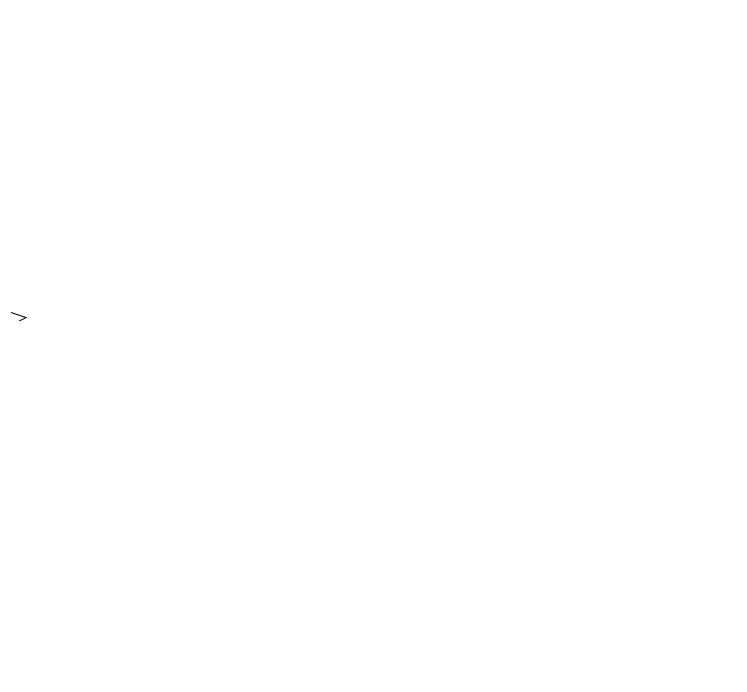
\includegraphics[width=\textwidth]{Images/cuore_18.pdf}
\end{minipage}
\hfill
\begin{minipage}{0.49\textwidth}
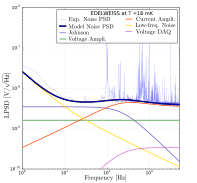
\includegraphics[width=\textwidth]{Images/edel_18.pdf}
\end{minipage}
\caption{Mesure expérimentale et modèle d'une densité spectrale de bruit à $18$ mK pour les électroniques CUORE (à gauche) et EDELWEISS (à droite) avec visualisation des contributions des différentes sources de bruits.}
\label{noise-sources}
\end{figure}

Il apparaît donc que l'électronique la moins bruyante est celle d'EDELWEISS. C'est donc avec cette électronique qu'il est convenu d'optimiser la résolution des détecteurs. Néanmoins, l'électronique EDELWEISS nécessite certaines modifications afin d'être utilisée avec une polarisation non nulle (remplacer la capacité par une résistance de charge). Cela étant à l'état de projet, on ne peut utiliser que l'électronique CUORE pour les mesures avec polarisation pour caractériser le détecteur RED10. Comme elle a également été caractérisé, cela ne pose pas de problèmes particuliers.

En utilisant la solution optimale trouvé avec l'analyse MCMC, il est possible de visualiser les contributions des différentes sources de bruits à la PSD de bruit totale, un exemple à $18$mK est présenté en figure \ref{noise-sources} pour les électroniques de CUORE et EDELWEISS. On constate bien que le bruit en courant de CUORE est très élevé et prédomine presque toute la gamme en fréquence. La fréquence de coupure du bruit Johnson, différentes pour les deux électroniques, illustre bien l'influence de la capacité du câblage. En effet, on a $f_{coupure} = 2\pi/(R_{NTD} C_{fil})$ en considérant $R_L\gg R_{NTD}$. On retrouve bien une fréquence de coupure plus élevée dans le cas de EDELWEISS qui possède une capacité de câblage plus faible (voir \ref{result}). Il est aussi possible d'étudier la prédominance des sources de bruits en fonction de la fréquence. Pour l'électronique d'EDELWEISS :
\begin{itemize}
\item en dessous de $10$Hz, le bruit est dominé par la contributions basse fréquence du bruit en tension $e_{B,C}$.
\item de $10$Hz à $100$Hz, le bruit totale vient se reposer sur le bruit intrinsèque au détecteur (bruit TFN et bruit Johnson du NTD). C'est exactement ce qui est recherché : on cherche à être limité par ces bruits thermiques détecteurs qui fixe la limite ultime atteignable.
\item au-dessus de $100$Hz, le bruit en courant de l'électronique d'amplification caractérisé par les coefficients $i_{A,B,C}$ devient prédominante.
\end{itemize} 

\begin{figure}[!ht]
\begin{minipage}{0.49\textwidth}
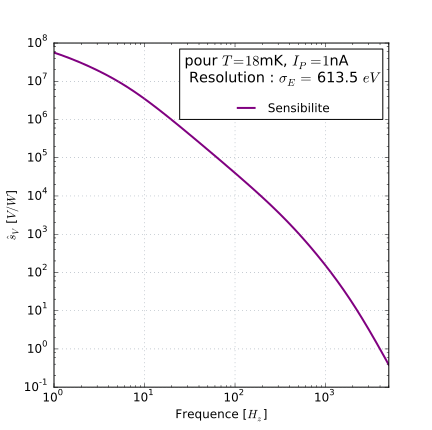
\includegraphics[width=\textwidth]{Images/sv_fin.pdf}
\end{minipage}
\hfill
\begin{minipage}{0.49\textwidth}
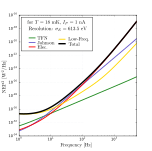
\includegraphics[width=\textwidth]{Images/nep_fin.pdf}
\end{minipage}
\caption{Simulation de la sensibilité (à gauche) et de la NEP (à droite) avec contributions des différentes sources de bruit pour l'électronique EDELWEISS à une température cryostat de $T=18$mK et un courant de polarisation de $1$nA.}
\label{nep-fig}
\end{figure}

\subsubsection{Tracé de la NEP et calcul de la résolution}
\label{nep-res}

Maintenant que l'on a contraint tous les paramètres du modèle de bruit, il est possible de finaliser le calcul de la résolution \ref{resolution} avec le calcul de la NEP \ref{nep}. La figure \ref{nep-fig} présente des graphes de sensibilité et de NEP du détecteur avec l'électronique EDELWEISS à $18$mK pour un courant de polarisation de $1$nA. La sensibilité est conforme avec la fonction de transfert d'un système thermique : il s'agit bien d'un passe-bas. Combiner selon la formule (\ref{nep}) cette sensibilité avec la PSD de bruit totale caractérisée précédemment permet d'obtenir une simulation de la NEP qui présente ses plus faibles valeurs entre $1$Hz et $100$Hz. 

%\begin{figure}[!ht]
%\begin{center}
%\includegraphics[width=0.7\textwidth]{Images/inte.png}
%\end{center}
%\caption{Simulation de la fonction $\frac{2}{\pi \times NEP^2(\omega)}$ qui apparaît comme intégrande dans la formule de la résolution (\ref{resolution}).}
%\label{inte}
%\end{figure}

Il est maintenant possible d'accéder à la résolution des cette configuration d'expérience avec la formule (\ref{resolution}). On calcule ici une résolution de $613.15$eV pour EDELWEISS, et une résolution de $1061.7$eV pour CUORE, avec une température de $18$mK et un courant de polarisation de $1$nA. On obtient bien une valeur inférieure avec l'électronique EDELWEISS, ce qui confirme davantage le choix de cette électronique pour l'optimisation de la résolution.

La formule du calcul de la résolution (\ref{resolution}) indique que les valeurs de NEP les plus basses contribuent le plus à la résolution. Même si intégrer sur une plus grande gamme de fréquence permet d'obtenir une résolution plus faible, le gain devient négligeable à mesure que la valeur de la NEP augmente.
On note que la NEP prend ses valeurs minimales au voisinage de $10$Hz : la majorité de l'information de la mesure est contenue dans une plage en fréquence allant de $0$Hz à environ $50$Hz. Le gain sur la résolution en intégrant au-delà de $50$Hz est infime. On cerne alors la plage de fréquence d'intérêt pour l'étude du signal. En observant les contributions des différentes sources de bruits à la NEP à la figure \ref{nep-fig}, on s'aperçoit que c'est le bruit basse fréquence qui domine dans cette plage de fréquence d'intérêt, suivi par le bruit Johnson de la résistance NTD. On comprend que pour diminuer davantage la résolution de ces détecteurs, il faut travailler à augmenter la sensibilité du système à un évènement ou réduire le bruit basse fréquence. Une partie de l'équipe Manoir travaille déjà à comprendre ce bruit basse fréquence.

\subsection{Caractérisation thermique du détecteur RED10}

Le détecteur RED10 n'est entré en possession du groupe Manoir que très récemment. Son design est identique à celui de RED1. La différence avec ce dernier repose dans le type de colle utilisée (colle de l'expérience CRESST) et les dimensions du NTD utilisé. Certains paramètres thermiques sont alors modifiés par rapport à RED1. Il est ainsi nécessaire de caractériser ces paramètres thermiques pour nouveau détecteur. On pourra ainsi étudier sa réponse à un évènement comme cela été fait avec RED1 dans les parties précédentes.

\subsubsection{Caractéristique courant-tension et forme du signal}

La caractérisation des paramètres thermiques utilise le modèle électro-thermique qui a été construit précédemment. On va vouloir ajuster les paramètres non contraints aux données expérimentales avec une analyse MCMC comme pour la caractérisation de l'électronique. Cette fois-ci, l'ensemble des paramètres libres est :
\begin{equation}
\Theta = (R_0, T_0, g_{ep}, g_k, g_{glue}, \epsilon, \tau_P)
\label{theta-red10}
\end{equation}
En effet, la nouvelle colle utilisée possède une conductivité $g_{glue}$ différente. La nouvelle géométrie du NTD (et également son dopage en neutron légèrement différent) va entraîner une modification de la résistance $R_0$ et température caractéristique $T_0$ présent dans l'équation (\ref{ntd}). Le changement de dimension impacte également le couplage électron-phonon $g_{ep}$ et le coefficient de conduction Kapitza $g_k$. A priori, les capacités thermiques volumiques de l'absorbeur et du NTD restent inchangées, ce qui permet de recalculer les nouvelles capacités thermiques à partir des dimensions connues du NTD. Il aurait été possible d'inclure celles-ci dans les paramètres libres mais le choix de les fixer a été favorisé afin d'éviter les problèmes de dégénérescence et ainsi mieux contraindre les paramètres.

Une étude préliminaire de la forme du signal (présenté à droite de la figure \ref{v2i-red10}) de RED10 a révélé que la décroissance de l'impulsion possède deux constantes de temps caractéristiques. Ce type de signal n'a jamais été observé sur les mesures de signal réalisée avec RED1 : il n'y a qu'un seul temps caractéristique de décroissance expliqué par la fuite thermique vers le cryostat depuis la bain d'électron avec un dépôt d'énergie de recul dans l'absorbeur. La présence d'un deuxième temps caractéristique pour RED10 ne peut s'expliquer que par la présence de phonons athermiques comme introduit dans la section \ref{omega}. Il s'agit de phonons ne se relaxant pas de suite dans l'absorbeur, mais passant dans le senseur NTD avant de s'y relaxer. Ils créent ainsi une élevation de température directement au sein du NTD. Le terme de source $\bm{F}$ de l'équation (\ref{ode-mat}) se réécrit alors :
\begin{equation}
\bm{F}(t-t_0) = 
\left( \begin{array}{c}
(1-\epsilon)E/C_a \\
0 \\
\epsilon E/C_e \\
0
\end{array} \right) \delta (t-t0)
\end{equation}
avec $\epsilon$ la fraction d'énergie de recul convertie en phonons athermiques. Les constantes de normalisation de la solution temporelle générale (\ref{eigein-solc-expr}) dépendent du terme de source $\bm{F}$ d'après (\ref{normal}) et diffèrent alors du cas de RED1 sans phonons athermiques. Cela a pour effet de mieux exprimer une nouvelle exponentielle, et donc un nouveau temps caractéristique, contenue dans la solution générale. Cette observation de deux temps caractéristiques pour le signal motive l'ajout de la fraction de phonons athermiques $\epsilon$ et de leur temps caractéristique de relaxation $\tau_P$ au paramètres libres du modèle.

On mesure sur RED10 les caractéristiques courant-tension et la forme du signal à un évènement de la radioactivité naturelle à courant de polarisation fixe $I_P=4$nA pour différentes températures allant de $18$mK à $30$mK. On étudie ainsi le comportment de RED10 dans l'état stationnaire (section \ref{steady-section}) et en régime temporel (section \ref{temporal}).
On effectue l'analyse par fonction de vraisemblance avec la méthode MCMC comme dans la section \ref{caract}. Les données expérimentales avec les modèles ajustés sont présentés sur la figure (\ref{v2i-red10}).

\begin{figure}[!ht]
\begin{minipage}{0.49\textwidth}
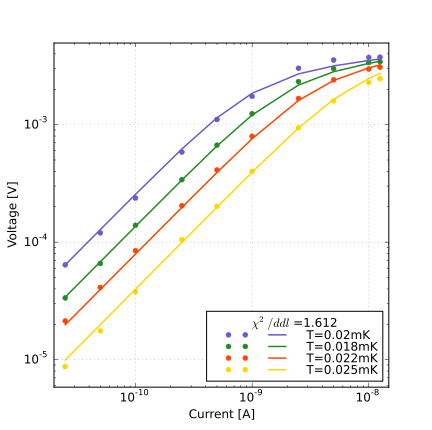
\includegraphics[width=\textwidth]{Images/v2i_red10.pdf}
\end{minipage}
\hfill
\begin{minipage}{0.49\textwidth}
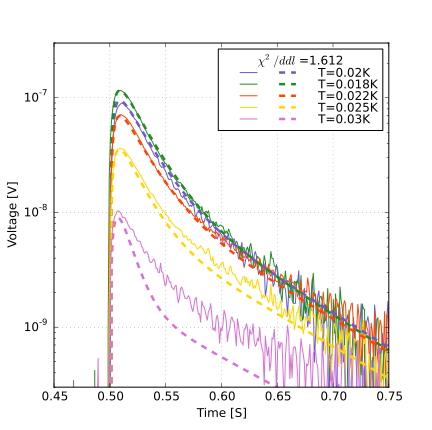
\includegraphics[width=\textwidth]{Images/pulse_red10.pdf}
\end{minipage}
\caption{Mesure expérimentale et ajustement par le modèle de la caractéristique courant-tension (à gauche) et  d'un signal créé par un évènement de radioactivité ambiante (à droite) pour le détecteur RED10.}
\label{v2i-red10}
\end{figure}

L'ajustement semble bon pour les deux types de mesure avec $\chi^2/ddl=1.612$. On observe néanmoins une difficulté de l'ajustement du pulse pour une température de $30$mK. La caractéristique courant-tension permet de contraindre les paramètres libres intervenant dans les équations de l'état stationnaire : $R_0, T_0, g_{ep}, g_k$. L'analyse de ces équations (\ref{steady}) nous donne que la partie linéaire de la caractéristique contraint surtout la valeur de résistance du NTD, et donc $R_0, T_0$. Le palier en tension à plus haut courant de polarisation provient d'un effet Joule excessif qui n'est alors plus compensé par la fuite thermique vers le cryostat. Le NTD augmente alors en température, perdant en résistance électrique avec un courant de polarisation constant, ce qui produit l'apparition du palier de tension. Son ajustement contraint ainsi les valeurs des conductivités $g_k$ et de couplage électron-phonon $g_{ep}$.

Pour ce qui est de la forme du signal, le modèle fait en effet apparaître deux pentes et donc deux temps caractéristiques. L'ajustement de ces deux pentes de décroissance contraint la fraction de phonon athermique $\epsilon$, et de manière plus générale, tous les paramètres intervenant dans le calcul des constantes de normalisation de la base propre des solutions (\ref{eigen-soluc}).
La montée en tension permet de contraindre le temps de relaxation des phonons $\tau_P$. En effet, pour une relaxation immédiate des phonons, le temps de montée serait infiniment grand (modulo la fréquence de coupure $(RC_{fil})^{-1]}$).

La méthode MCMC donne alors les contraintes suivantes pour RED10:

\begin{align}
R_0 &= (11.6 \pm 0.4)&[\Omega] \\
T_0 &= (2.72 \pm 0.01) &[K] \\
g_{ep} &= (21.1 \pm 4.4) &[W/K^6/cm^3] \\
g_k &= (2.77 \pm 0.1) \times 10^{-4}&[W/K^4/mm^2] \\
g_{glue} &= (7.46 \pm 1.67) \times 10^{-4} &[W/K^{n_g}/mm^2] \\
\epsilon &= (0.202 \pm 0.001)  & [fraction]\\
\tau_P &= (4.03 \pm 0.03) \times 10^{-3} &[s]
\end{align}

Ces valeurs de paramètres thermiques sont du même ordre de grandeur que celles correspondantes à RED1. Il est important de mettre en évidence la forte portion de phonons athermiques d'environ $20\%$ qui est à comparer à leur absence complète avec le détecteur RED1. Il s'agit d'une observation encore inédite pour ce type de détecteur. Leur présence élevée se traduit par une accélération du signal en tension et donc une augmentation de la gamme de fréquence d'intérêt du signal introduit dans la section \ref{nep-res}. De plus, les phonons athermiques ne sont pas affectés par la capacité de l'absorbeur, et transmettent directement l'ensemble de leur énergie au NTD. La compréhension et l'augmentation du taux de phonons athermiques permettrai ainsi d'abaisser la résolution du détecteur. On a ainsi découvert une nouvelle voie d'optimisation des détecteurs encore non considérée au sein de la collaboration EDELWEISS.

\subsubsection{Bruit et résolution de RED10}

Comme RED10 est complètement caractérisé du point de vue thermique, et que l'électronique CUORE utilisée pour les mesures l'est également, nous sommes en mesure de simuler le spectre de bruit lié à RED10 que l'on compare à la mesure expérimentale. La figure (\ref{noise-red10}) présente la modélisation et la mesure expérimentale de la PSD du bruit de RED10 à courant de polarisation de $4$nA pour une température de $22$mK. On notera qu'un filtre de Bessel est appliqué à la mesure, et au modèle, ce qui explique la coupure apparaissant à partir de $2$kHz.

\begin{figure}[!ht]
\begin{center}
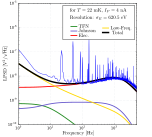
\includegraphics[width=0.55\textwidth]{Images/modexp.pdf}
\end{center}
\caption{Mesure expérimentale d'une densité spectrale à $22$ mK avec RED10 comparée à une simulation du modèle construit.}
\label{noise-red10}
\end{figure}

Le modèle et la mesure décrivent des évolutions très similaires. On retrouve effectivement la présence d'un bruit basse fréquence élevé qui domine jusqu'à $15$Hz. C'est ensuite le bruit en courant qui prédomine sur le reste de la gamme de fréquence. On notera qu'on effectue ici une mesure de bruit avec courant de polarisation, il serait donc incorrect de vouloir comparer le bruit en courant présenté de RED10 avec les bruits en courant de RED1 obtenus sans courant de polarisation. On observe toutefois un léger glissement du modèle par rapport aux données expérimentales vers les basses fréquences. Cela peut être expliqué par la sous-estimation du bruit basse fréquence déjà observé pour l'électronique de CUORE à la figure (\ref{rainbow-plot}). L'excès de bruit basse fréquence provient également du taux important d'évènements muons durant les mesures : malgré les coupures effectuées en analyse, on récupère toujours une partie de la décroissance des signaux, ce qui participe à amplifier les basses fréquences du spectre mesuré.

La mesure de résolution expérimentale s'effectue à partir des PSD de bruit et de la mesure d'un signal. En effet, renormaliser l'amplitude du signal et lui appliquer une méthode de Welch permet d'estimer la sensibilité en signal du détecteur RED10. La renormalisation nécessite également de connaître la conversion entre l'énergie déposée dans l'absorbeur par un évènement et l'amplitude du signal mesurée. Cette calibration s'effectue à l'aide de l'interaction des muons cosmiques avec l'absorbeur. L'énergie qu'ils déposent dans l'absorbeur est égale à $18$MeV. La mesure de l'amplitude en tension d'un signal muon permet donc d'en déduire le facteur de conversion nécessaire à la renormalisation d'un signal. L'application de l'analogue discrète de la formule (\ref{resolution}) à un spectre de bruit et la sensibilité calculée précédemment  permet l'évaluation d'une résolution expérimentale. 

\begin{figure}[!ht]
\begin{center}
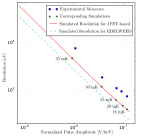
\includegraphics[width=0.55\textwidth]{Images/resamp_fin_fin.pdf}
\end{center}
\caption{Caractéristique Résolution-Amplitude de signal pour le détecteur RED10 pour un courant de polarisation de $4$nA avec des températures allant de $18$mK à $30$mK.}
\label{amp-res-red10}
\end{figure}

On présente sur la figure (\ref{amp-res-red10}) les résolutions en fonction de l'amplitude du signal pour différentes températures à courant de polarisation fixé. Les résolutions expérimentales sont plus élevées que les résolutions simulées. Cela s'explique par la déviation entre modèle et mesure de bruit observée en figure (\ref{noise-red10}): le bruit basse fréquence modélisé est plus bas qu'en réalité, d'où la prédiction de résolutions plus basses. L'amplitude des pulses permet d'estimer la sensibilité de RED10 au signal. Hormis la mesure à $30$mK dont le signal était déjà mal modélisé, les valeurs d'amplitude simulées et réelles sont quasiment identiques. De plus, comme les deux ensembles de points présentent une évolution de la résolution en fonction de l'amplitude très similaire, on en déduit que le modèle est en bonne adéquation avec la réalité expérimentale. Une étude de la différence sur le bruit est encore nécessaire pour obtenir une adéquation complète de modèle et de l'expérience.

On notera qu'on a effectué les mesures avec l'électronique de CUORE. La simulation de la caractéristique résolution-amplitude est tracée pour les deux électroniques CUORE et EDELWEISS. On note que cette dernière permet de gagner quasiment un facteur 2 sur la valeur de la résolution (l'amplitude reste inchangée). Ce qui est cohérent avec le faible niveau de bruit de EDELWEISS par rapport à celui de CUORE.

\subsection{Optimisation du détecteur RED10 et perspectives}

Un modèle électro-thermique a été construit et testé avec RED10. Même si quelques paramètres méritent d'être davantage affinés pour avoir un meilleur ajustement, nous pouvons réaliser une optimisation préliminaire du détecteur RED10. On présente à la figure \ref{optim} une simulation de la résolution de RED10 en fonction de courant de polarisation parcourant son NTD pour différentes température de cryostat. La simulation est effectuée avec l'électronique EDELWEISS qui possède le niveau de bruit le plus faible, et on abaisse la température de la résistance de charge à la température de la chambre de mélange pour réduire son bruit Johnson (ce qui sera réalisé dans ces prochains mois).

On observe qu'il existe un optimum de courant correspondant à chaque température permettant de minimiser la résolution. En effet, si on polarise trop la thermistance NTD, la chaleur produite par effet de Joule ne peut plus être évacuée efficacement par la fuite thermique. La température du NTD devient haute et donc sa valeur baisse, ce qui affecte la sensibilité du système. Ce même effet est observé lors du tracé de la caractéristique courant-tension en figure \ref{v2i-red10}. À trop faible courant, le senseur NTD n'est plus assez polarisé pour convertir efficacement le signal chaleur en un signal tension : la sensibilité chute également. Quelque soit le courant de polarisation utilisé, on obtient toujours la résolution la plus basse avec la température la plus faible. La formule de la résistance du NTD (\ref{ntd}) permet d'expliquer qu'on a effectivement une plus grande sensibilité du signal à basse température : la dérivée de la résistance par rapport à la température y prend ses valeurs maximales (de manière absolue). De plus, descendre en température permet de réduire tous les bruits TFN, et le bruit Johnson de la thermistance NTD, ce qui améliore davantage la résolution.

\begin{figure}[!ht]
\begin{minipage}{0.49\textwidth}
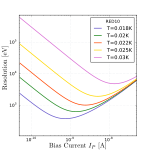
\includegraphics[width=\textwidth]{Images/red10_i.pdf}
\end{minipage}
\hfill
\begin{minipage}{0.49\textwidth}
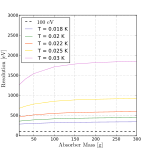
\includegraphics[width=\textwidth]{Images/red10_mass.pdf}
\end{minipage}
\caption{(à gauche) Simulation de la résolution de RED10 en fonction du courant de polarisation pour différentes températures. \\ (à droite) Simulation de la résolution à courant de polarisation optimisé en fonction de la masse de l'absorbeur pour différentes températures. Le design considéré est le même que celui de RED10, on change seulement la masse de l'absorbeur en ajustant le courant de polarisation pour obtenir la résolution la plus faible.}
\label{optim}
\end{figure}

L'étude de RED10 s'est entièrement réalisée pour un courant de polarisation de $4$nA, ce qui correspond au courant optimal d'une température d'environ $24$mK. Il aurait donc été possible d'obtenir de meilleures valeurs de résolution en ajustant pour chaque température le courant de polarisation. Ainsi, il sera important, dans le futur, de bien déterminé le courant de polarisation optimum d'un détecteur suivant les conditions de mesures.

La recherche de matière noire légère nécessite de mettre au point une nouvelle génération de détecteur avec de très bas seuil de détection. Pour cela, il est nécessaire de travailler sur le design des détecteurs. Il faut par exemple étudier le comportement du détecteur selon la géométrie du NTD, la masse de l'absorbeur ou encore l'emplacement des fuites thermiques. On présente sur le graphe à droite de la figure \ref{optim}, une simulation de la résolution d'un détecteur en fonction de la masse de l'absorbeur. On notera que le courant de polarisation est ajusté pour chaque point afin de tracer une courbe de résolution déjà optimisée. D'après la formule (\ref{capa}), il serait intéressant de réduire la capacité thermique de l'absorbeur $C$, en abaissant sa masse, afin de provoquer une plus grande élévation en température $\Delta T$, et ainsi amplifier le signal chaleur. D'après la simulation, cette amplification du signal chaleur n'apparaîtrait que pour de très petites masses de détecteur, et resterait très modeste pour les faibles températures. 

On comprend maintenant qu'on reste limité pour le moment par un autre aspect du détecteur. Dans le futur, l'optimisation du détecteur va passer par l'étude du comportement en fonction des dimensions du la thermistance NTD et des surfaces de conduction thermiques. Il apparaît déjà qu'il faudrait réduire les capacités thermiques des différents bains tout en maximisant les liens thermiques. 


%
%% Ionization Theory
%% Chapter Electrodes

\chapter{Electrodes Design with Electrostatic Simulation} % Main chapter title

\label{ChapterElectrodes} % Change X to a consecutive number; for referencing this chapter elsewhere, use \ref{ChapterX}

%----------------------------------------------------------------------------------------
%	BEGING CHAPTER
%----------------------------------------------------------------------------------------

Let me tell you about my work with an electrostatic simulation software called COMSOL.
That was quite nice. Just designing the detector and the aluminium electrodes with a beautiful and efficient interface.
Thanks to that, I could simulate a lot of configuration and geometry to probe for the finest results out there.
Finest meaning a lot of fiducial volume, good charge collection, and low electric capacity.
A usual impossible to solve problem which lead to a lot of trade-off in itself, without adding the issues about the heat channel.
But hey, I could obtain some nice plots and tables, check them out.


\section{Electrodes as Sensors for the Ionization Channel}

\subsection{Basics of the Ionization channel}

The ionization channels aims at converting the ionization of the germanium into a voltage signal.
This is done with the use of aluminium electrodes acting as the terminals of a capacitor of capacitance $C$. When collecting an electric charge $\Delta Q$, a voltage $\Delta U$ is created across the capacitor such as:

\begin{equation}
C = Q \times U \quad \Leftrightarrow \quad U \times = \frac{C}{Q}
\label{eq:capacitor-basic}
\end{equation}

A high sensitivity of the ionization channel means that the created voltage $\Delta V$ is maximized. The equation \label{eq:capacitor-basic} shows that a low capacitance $C$ of the electrodes and a high collection of electric charge $\Delta Q$ increase the ionization channel response. While the amount of electric charge $\Delta Q$ can depend of the electric field shape, in the case of a theoretically perfect charge collection, the number of electron-hole pairs created and collected only depends on the recoil energy $E_R$ of the interacting particle $i$ and the associated quenching factor $Q^i(E_R)$. This factor depends only on the material used as absorber, in our case Germanium.
The capacitance depends on the design of the detector, and is the one of the main quantities used to quantify the performance of a detector design.


\subsection{Germanium as Semiconductor}

The material used as absorber for the detectors is semi-conducting High Purity Germanium [ref?].
This paragraph focuses on its characteristics and also compares it to materials used by others experiments using bolometers.

The use of semi-conducting Germanium as an absorber was first proposed by Taverdale? and Evvan [80, Emeline].
Along with an increase in temperature, a semi-conducting germanium also features a phenomenon of ionization caused by a particle interaction. Such electronic and nuclear recoils form electron-hole pairs of average energy $\epsilon = 3 eV/pair$. This energy corresponds to the gap energy separating the valence and conduction electronic bands in the germanium in its semi-conducting state accessible for temperature below 77K.

In order to understand the physical properties of a semi-conductor, we can consider the theory of energy bands. In a solid material, at rest electrons are occupying the lowest state of energy according to their fermion nature. This lowest state of energy are strongly linked to the nucleus, forming the valence electronic band of energy. Higher energy states are able to interact with neighboring atoms and compose the conduction electronic band of energy.
conducting, not conducting, semi-conductor. Small gap. blablabla

The semi-conducting properties of a germanium crystal heavily depends on the impurities affecting it. With the Germanium element being of valence 4, there exist two kind of impurities:
\begin{itemize}
	\item acceptor impurities of valence 3 producing a p-type germanium,
	\item donor impurities of valence 5 producing an n-type germanium.
\end{itemize}
These impurities creates intermediary energy steps in the semi-conducting germanium band gap accessible to electric charges (as seen in figure \ref{fig:conduction-bands}). The presence if this intermediate accessible energy bands has several consequences on the ionization channel. It reduces the energy necessary to create an electron-hole pair, thus creating additional noise and biasing for the ionization channel. Then, it creates a trapping phenomenon which prevent electric charge carriers from reaching the electrodes. With trapped charges in the crystal, a counter electric field slowly generates, reducing the sensitivity of the electrodes. Finally, these impurities lower the global resistivity of the germanium crystal and increase the leakage current.
The semi-conducting germanium use as absorber thus should contain the lowest amount of impurities in order to have a detector with good performances.
The study of the trapping in EDELWEISS detector and the impact of impurities is presenting in [ref quentin 80].
We define $N_a$ and $N_d$ as the number of acceptor and donor impurities respectively. We  can have access (how?) to the absolute difference of this quantities $|N_a - N_d|$ which determine the number of available charge carriers.
The material used as absorber is High-Purity Germanium (HPGe) with an estimated:
$$ 10^{9} < |N_a - N_d| < 10^{10} \textsf{cm}^{-3}$$
which corresponds to less than one impurity atom for $10^{12}$ germanium atoms. With this material, low leakage currents of few pA can be achieved for the usual operating  electric field range of a few V/cm.

Ok, so here might be some mumbo jumbo concerning the p-n junction in a semi-conductor. Is it useful ? idk.
A recurring term is "depletion depth" which apparently is inversely proportional to the impurity concentration.
A germanium crystal with good performance should present a high resistivity obtainable with a high depletion depth.
As a result, the EDELWEISS and RICOCHET experiment use high purity germanium (HPGe) with special treatment [ref?] leading to a low impurity concentration of less than $10^{10}$ atoms.cm${-3}$ (1 impurity for $10^{12}$ germanium atoms) whereas a normal germanium crystal possesses a concentration of about $10^{13}$ atoms.cm${-3}$.

Comparing the germanium to silicium:
\begin{itemize}
	\item higher Z, so better quenching factor [lindhard]
	\item denser material, better for exposure
	\item low impurities, big depletion region
	\item low ionization energy (gap?)
	\item high conductivity (?)
\end{itemize}

\begin{figure}
\centering
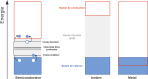
\includegraphics[width=\linewidth]{Figures/Electrodes/conduction_bands.pdf}
\caption{Scheme of the conduction bands for semiconductor, insulator and conductor materials.}
\label{fig:conduction-bands}
\end{figure}


\subsection{Electric Charge Drifting in Crystal}

{\color{red}
Alex B. biblio here.
Also explainin trapping, charge collection.
}

The study of charge migration in EDELWEISS germanium crystal is presentend in [ref Emeline 82] taking into account the crystallographic structure of the germanium crystal. In this study, Alex.B simulates numerically the drifting of eletrons and holes in a 200g FID Edelweiss detector with bulk interaction of gamma-rays of energy 348keV. The charge trajectories are presented in the figure \ref{fig:charge-drifting}. He also follows the generation of the voltage signal on the electrodes. This is consistent with Ramo field theory which will be described later.

When interacting with the atoms of a germanium crystal, a particle deposits a so-called recoil energy. The word "recoil" references to the elastic diffusion of the incoming particle on a germanium nuclei, this is a nuclear recoil, or the elastic diffusion of the electronic cloud of a germanium atom, this is an electronic recoil. A fraction of the recoil energy is used for the creation of electron-hole pairs, this process is known as ionization. This fraction is called quenching factor $Q$ whose value depends on the recoil type, the incoming particle, and the recoil energy. When a electron-hole pair is created, a valence electron is going into the conducting band of the semi-conducting germanium crystal (as illustrated in the figure \ref{fig:conduction-bands}) while a hole appears in the valence band. Following a recoil, electrons can excited with energies much greater than the germanium gap energy. However, such electrons relaxes by phonon emission and creation of new electon-hole pairs. We can consider that after relaxation, the number of electron-hole pairs $N^j$ induced by a recoil of type $j \in {e(lectronic), n(uclear)}$ is expressed as:
\begin{equation}
\label{eq:number-pairs}
N^j = Q^j \left( E_R \right) \frac{E_R}{\epsilon}
\end{equation}
with $\epsilon$ the average energy necessary for the formation of an electron-hole pair and $Q^j$ the quenching factor function of $E_R$ the recoil energy.

The average energy $\epsilon$ contained in a pair is greated than the germanium gap band of $0.67\textsf{eV}$ as it also take into account the momentum associated to the interaction between the pair and the crystal. The figure \ref{fig:band-structure} represents the lower energy of the valence band and the higher energy of the conduction band in a germanium crystal depending on the orientation (orientation of what ? germanium crystallography, electron momentum ?). While the absolute lowest energy of the conducting band, at [111] and the highest energy of the valence band, at [000], are separated by the germanium gap energy of $0.67\textsf{eV}$, this extremum does not correspond to the same orientation $\bm{k}$, the germanium gap is indirect. An electron can transition into the conducting band with the transfer of a momentum $\bm{k}$ from the phonon in order to respect the conservation of momentum and energy (as described in [ref quentin 87]). In the end, the average energy of a pair in germanium is estimated to [ref necessary]:
\begin{equation}
\label{eq:energy-pair}
\epsilon = 3 \textsf{eV}
\end{equation} 

The number of created pairs $N^j$ is subject to fluctuation and thus impose itself as an intrinsic limit to the resolution of the ionization channel. The number of pairs $N^j$ should be expected to follow a Poisson distribution of standard deviation $\sigma(N^j) = \sqrt{N^j}$. However, the observed fluctuation are lower than expected and could be explained by a correlation of the relaxation process of the phonons and electron-hole pairs. The paper [ref 85 quentin] propose a standard deviation expressed as:
\begin{equation}
\sigma(N^j) = 2.35 \sqrt{F \epsilon E_R / Q(E_R)}
\end{equation}
with an introduced Fano factor $F$ of about 0.1 for the germanium. Considering the current range of ionization channel resolution, the fluctuation of the number of pairs created by ionization could be limiting with $\sigma(N^j) \approx 300\textsf(eV)$ which could be obtained for (electronic) recoil energy greater than $300\textsf{keV}$. As we are interested in the lowest energy range and the experiments presented in this work use calibration peaks of energy $\approx 10keV$, the impact of these fluctuation are negligible (especially considering other effects such as the trapping, the electronic noise, etc..).

As will be seen in the next paragraph, the voltage signal generated at the electrodes is based on the charge movement and is only partially affected by the fact that the charge is indeed collected by the electrode. The signal last a few microseconds with a speed of the charge carrier of a few cm/$\mu$s.
Also, the electrons tends to travel following inter-valleys in the crystal with a certain angle while the hole travel independently of the crystal orientation. This is problematic for a good charge collection and "herding" of the electron by the electric field.


\begin{figure}
\centering
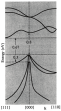
\includegraphics[height=0.5\textheight]{Figures/Electrodes/band_structure.pdf}
\caption{Scheme of the band structure in a germanium crystal.}
\label{fig:band-structure}
\end{figure}

\begin{figure}
\centering
\includegraphics[height=0.5\textheight]{Figures/Electrodes/charge_drifting.pdf}
\caption{Scheme of the band structure in a germanium crystal.}
\label{fig:charge-drifting}
\end{figure}


\subsection{DAQ and electronics for ionization}

The electronics used for the ionization and the heat channel uses Junction Field Effect Transistor (JFET) which are operated at a low temperature of 100K inside the cryostat.
Some mumbo jumbo about the bolo-box (is it necessary ?).
The figure \ref{fig:electronics-scheme} show the scheme of the cold electronics for the heat channel (on the left) and the ionization channel (on the right).

\begin{figure}
\centering
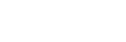
\includegraphics[width=\textwidth]{Figures/Electrodes/electronics_scheme.pdf}
\caption{Scheme of the cold electronics readout for the heat channel (left) and the ionization channel (right)}
\label{fig:electronics-scheme}
\end{figure}

In most experiments (source?), the ionization channel readout is done with the integration of the drifting charge current on the feedback capacitance of a charge amplifier. However, the EDELWEISS electronics directly measures the electric potential of the electrodes with a voltage amplifier. As each electrode is considered as a terminal of a capacitor $C_{electrode}$, the measured voltage is:
\begin{equation}
U = \frac{Q}{C_{electrode}}
\end{equation}
with $Q$ the drifting charge seen by the electrode.
Compare with a charge amplifier, the voltage amplifier does not involve any resistor in the amplification scheme, resulting a lower noise. However, the use of a voltage amplifier is only possible with a low leakage current, lower than 0.1fA (good for EDELWEISS, but is this possible for RICOCHET with operation on surface).

The ionization channel readout being based on the collection of electric charges, the renewal of the electric potential of the electrodes is necessary to maintain the voltage bias of the detector and to prevent the signal from leaving the readout range [-32000, +32000]. This operation, called a “reset”, consists in linking each electrodes to a polarization circuit of fixed electric potential. The linking is assured with mechanical relays (motivated by publication?) represented as a switch on the electronics scheme. The period of the resets is of a few seconds and should be adjusted empirically to the operated detectors and the event rates. In the case of surfaces operation at IP2I, the event rate is high and lot of charges are accumulated which needs for a shorter period than an underground operation at the LSM.
One should note the double switch of the mechanical relays accompanying each reset induces an artifact signal on both the heat and ionization channel. While easily discriminable from real events, these artifact signal result in dead time during which the detector is not available for valid event recording. Thus a short period of reset is not wanted.

While the majority of the electric charges produces by the ionization process are collected by the electrodes, some become trapped in the crystal (impurities) or on the surfaces of the crystal. These trapped charges are slowly accumulating and creating a counter electric field in the absorber. This results in a lower electric field perceived in the bulk of the detector which hampers a correct charge collection and decreases the sensitivity of the electrodes.
A procedure called “maintenance” is used to periodically shake up the trapped charges. These maintenances prevent, or at least slow significantly, the counter field build-up in the detector. A maintenance consists of a minute of multiples relay switches and relay changeovers. This procedure continuously invert the voltage bias in the detector, eventually destabilizing the trapped charges which are left to drift and collection in the electrodes.
During a maintenance, the detector is not available for data taking. The frequency of maintenance should be low to lower the dead time. For above ground operation, the usual maintenance period is of about 30 minutes and should be empirically adjusted to the detector and the event rate.

While a maintenance shakes up the majority of the trapped electric charges, a small fraction is not affected and participates to build up the counter field. These remaining charges are deeply trapped and need for a stronger perturbation to be freed. The detector is therefore periodically submitted to a procedure called "regeneration" aiming at a full reset of any passive electric field in the germanium crystal. With the electrodes being grounded, an intense gamma-ray radioactive source irradiates the detector. The high frequency of high energy recoils produces ionization in the whole crystal which eventually neutralize the accumulated space charges. 
As for the reset and maintenance procedures, the period between two regenerations should be empirically adjusted to the measured charge accumulation while not too frequent to avoid supplementary dead times. For above-ground operation, regeneration are realized ever two days (with a 1Cu cesium source).

Between each maintenance, the detector stays floating. The common noise can be subtracted when considering the charge conservation for all the electrodes:
\begin{equation}
\label{eq:charge-conservation}
A + B + C + D = 0
\end{equation}
With a linear combination of the raw ionization channels (A,B,C,D), we obtain new quantities (A’, B’, C’, D’) corrected from this common noise:
\begin{equation}
\label{eq:common-noise-subtraction}
A’ = \frac{3}{4} A - \frac{1}{4} \left( B + C + D \right)
\end{equation} 
The decrease of the noise level can be appreciated in the figure \ref{fig:ionization-noise} showing the noise spectrum affecting the different ionization channels before and after linear combination.

\begin{figure}
\centering
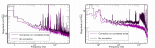
\includegraphics[width=\textwidth]{Figures/Electrodes/ionization_noise.pdf}
\caption{Average noise amplitude (in nV / Hz ) as a function of frequency of the
ionization channel for an EDELWEISS detector. The black histogram corresponds to the
noise before the correlated noise correction and the purple histogram to the noise after
the correction. Left: frequencies below 500 Hz. Right: high frequency part. [Emeline caption]}
\label{fig:ionization-noise}
\end{figure}

The ionization channel readout is sampled at an initial 100kHz. This means the period of the  measurement points is 10$\mu$s which greater than the estimated time span of an ionization signal of a few $\mu$s [ref necessary Alex.B ?]. As a result, an ionization signal is recorded as an Heaviside function. No information can be obtained on the shape of the signal.
The high readout sampling was historically chosen in EDELWEISS for the purpose of triggering on the ionization channel with a good temporal resolution (is it true ?). The highly sampled ionization signal is then averaged in order to produce a signal of frequency $f_s$ of about 400Hz. This lower sampling is able to record the information contained in the ionization Heaviside signal (its amplitude mainly) while being lightweight in term of disk space, which is essential considering the recording and processing resources at our disposal. The saved ionization signal of sampling frequency $f_s$ is composed of points which are averages of $100kHz/f_s$ points. The saved signal is therefore a skewed Heaviside-like function (more info needed? Is this work using this fact?).

Should I talk about the HEMT technology ? The expected resolution and noise level ?


\subsection{Aluminum Deposition}

*Stefanos biblio here.*

The electrodes of the detectors are made by depositing aluminium on the surface of the germanium crystal. The aluminium deposition is carried out by the research group at CSNSM at Orsay. The deposition processes are still being improved.

The germanium crystal is placed in vacuum chamber where its surface is altered with beams of vaporized atoms (hydrogen, aluminium, xenon…). 
In order to prevent the surface leakage, a highly resistive layer is created under the aluminium electrodes. It is a 60 to 80 nm deep amorphous layer of hydrogenated germanium.

Two techniques are used for the detectors presented in this work: evaporation with mask and the (photo)lithography.
A solid mask can set between the beam source and the crystal in order to shape the altered surface. In the case of concentric circular electrode, the mask (presented in figure {fig:mask-evaporation}) consists in several curved slits which allow the passage of vaporized aluminium. By rotating the mask during the process, the aluminium is deposited in a ring pattern on the germanium.
Another method to control the shape of the electrode is to use photolitography. First, the whole surface of the crystal is covered with a layer of aluminium. Then, the aluminium is coated with a chemically-protective wax. The negative of the electrode pattern is carved in the wax coating with the use of lasers (hence the name of the procedure). Once done, the germanium crystal face is immersed in chemical solution reactive with aluminium. Only the aluminium protected by the wax (patterned as the desired electrode design) is left on the surface. Finally, the wax coating is removed with an other chemical.

Advantages and Inconvenient of the 2 techniques ?
-Mask during evaporation is more precise and quicker but can only be use for simple patterns  with the cylindrical symmetry of the crystal.
-Photolitography is a longer process, and may be less precise (chemical attack of the aluminium?) but can be used for any pattern desired. Useful in the case of square grids.
- Also, some constraints on the minimum width of the electrodes ?

Leakage current exist on the surface of the crystal thanks to possible defects (ref edelweiss?). After depositing the electrodes, the bare germanium surfaces are etched with a XeF2 pulsed beam in vacuum chamber. The surface of the germanium is altered according to the following equation:
$$Ge + 2XeF_2 \longrightarrow GeF_4 + 2Xe$$
The xenon gas is removed and the fluoarated germanium surface is able to hold much higher voltage bias.

Now that the aluminium electrodes were deposited on the germanium crystal, it is possible to proceed with the cabling. The fragility of the germanium and the shallow aluminium layers motivate the use of wire-bonding as cabling technique. 

*description wire-bonding machine*

In the case of simple electrodes (full planar detector), several wires link the top (and bottom) electrodes to a conductive pad on the detector copper chassis. The conductive pad is then cabled to the ionization electronics.
With more complex design (fully interdigitized), wires are used to connect different aluminium patches, essentially imposing the same electric potential is those. With two wire bridges, It is possible to create interleaved electrodes with a biasing scheme based on the co-planar grid technique for event localisation [ref emeline 86], but more on that later.


\subsection{Luke Neganov effect}

When electric charges drift under the influence of the applied electric field in the germanium crystal, phonons are created and eventually participate to the heat signal. This process is called the Luke-Neganov [ref 63 emeline]. This phenomenon happening in semi-conductors is analogous to the Joule Effect present in conductors. 
The drifting electrons constantly dissipate their energy to the phonons bath. As the electrons stay in motion and are eventually collected by the electrodes, the electric field must provide a work $W$ compensating the energy loss going into the heat channel.
This work required for a single electron-hole pair is expressed as:
\begin{align}
W &= q_{e^{-}} \int_{ \vec{r_i} }^{ \vec{r_{e,f}} } \vec{E} d\vec{r} - q_{h^{+}} \int_{ \vec{r_i} }^{ \vec{r_{h,f}} } \vec{E} d\vec{r} \\
&=  -e \int_{ \vec{r_i} }^{ \vec{r_{e,f}} } \frac{\partial V}{\partial \vec{r}} d\vec{r} + e \int_{ \vec{r_i} }^{ \vec{r_{h,f}} } \frac{\partial V}{\partial \vec{r}} d\vec{r} \\
&= e \left( V(\vec{r_{h,f}}) - V(\vec{r_{e,f}}) \right)
\end{align}
where $q_{e^{-}} = e = - q_{h^{+}} $ represent the electric charges and $\vec{r_{i,f}}$ is the final position of the electric charge $i \in \{e^{-}, h^{+}\}$. Therefore, the energy generated by the Luke-Neganov (for a single pair) depends solely on the electric potential at the end of drift positions for the electron $\vec{r_{e,f}}$ and the hole $\vec{r_{h,f}}$.


The Luke-Neganov effect boosts the heat channel by adding a Luke-Neganov energy $E_{Luke-Neganov}$. For a recoil of type $j \in \{ e, n\}$ generating a number of electron-pairs $N^j$, the expression of this energy is:
\begin{equation}
E_{Luke-Neganov} = e \sum_{i=0}^{N^j} \left( V(\vec{r_{h,f}^i}) - V(\vec{r_{e,f}^i}) \right)
\end{equation}
A useful, and mostly accurate, approximation is to consider that all the charges end their drift by being collected at the electrodes polarized at potential $V_+$ and $V_-$. Thus, a simpler expression of the boost in energy is:
\begin{equation}
E_{Luke-Neganov} = N^j e (V_+ - V_-) = N^j e \Delta V
\end{equation}
The Luke-Neganov effect is proportional to the number of pairs $N^j$ created in the ionization process and the voltage bias $\Delta V$ of the detector. Using the equation \ref{eq:number-pairs}, we can express the boost as a function of the recoil energy $E_R$ and the associated quenching factor $Q^j$:
\begin{equation}
E_{Luke-Neganov} = Q^j \frac{E_R}{\epsilon} e \Delta V
\end{equation}
A useful simplification is to consider that $e / {\epsilon} = 1/3 \textsf{V}^{-1}$,  and to have a final expression of the Luke-Neganov boost as:
\begin{equation}
\label{eq:nl-boost}
E_{Luke-Neganov} = Q^j E_R \frac{\Delta V}{3}
\end{equation}
We see that for the same recoil energy $E_R$, an electronic recoil will benefits more than a nuclear recoil from the boost according to the comparison of  their quenching factor $Q^e > Q^n$. This is very important to keep in mind when reconstructing the recoil energy $E_R$ from the measured heat energy $E_{heat}$ as it is a function of the deposited recoil energy $E_R$ and the recoil type $j$:
\begin{align}
E_{heat} (E_R, j ) &= E_{R} + E_{Luke-Neganov} ( E_R, j) \\
&= E_R \left( 1 + Q^j(E_R) \frac{\Delta V}{3} \right)
\end{align}

*more on that now or later ? Kevee, kevnr, use of the Ei and Ec to deduce Q and Er*


\subsection{Shockley–Ramo theorem}

[ref quentin 100 101 102]
The signal induced on the electrodes of a detector does not corresponds to the collection of the drifting charges (when the charges reach the electrodes) but rather corresponds to the induced current starting from the moment the electron-pairs are created by a recoil. Indeed, when a charge is moving in the vicinity of an electrode, it induces an instantaneous electric current by affecting the electrostatic field lines ending on the electrode. 
[wiki after]
The Shockey-Ramo theorem states that the current $i$ induced on a given electrode due to the motion of a charge is given by:
\begin{equation}
I = E_v q v
\end{equation}
where $q$ is the charge of the particle, $v$ its velocity and $E_v$ the component of the electric field in the direction of $v$, under the following conditions: charge removed, given electrode raised to unit potential, and all other conductors grounded. This theorem ensues from Gauss theorem.
This theorem can be integrated to access the induced charge on a given electrode $k$:
\begin{equation}
\label{eq:ramo-theorem-integrated}
Q_k = - q \Phi_k(\vec{r})
\end{equation}
with $\Phi_k(\vec{r})$ the weighted potential of the electrode $k$. This weighted potential is obtained in the same conditions as $E_v$. (figure of such potential for an electrode?).
In the case of a drifting charge $q$ of initial position $\vec{r_{q,i}}$ and final position $\vec{r_{q,f}}$, the total integrated charge induced on the electrode $k$ is:
\begin{equation}
Q_k = q \left( \Phi_k (\vec{r_{q,f}}) - \Phi_k (\vec{r_{q,i}}) \right)
\end{equation}
The Shocley-Ramo theorem benefits from the superposition theorem such that it is possible to express the signal induced by a number $N$ of electron-hole pairs:
\begin{align}
Q_k &= \sum_{n=1}^{N} \left( Q_k^n(e^-) + Q_k^n(h^+) \right) \\
&= \sum_{n=1}^{N} -e \left( \Phi_k^n (\vec{r_{e,f}}) - \Phi_k^n (\vec{r_{e,i}}) \right) +e \left( \Phi_k^n (\vec{r_{h,f}}) - \Phi_k^n (\vec{r_{h,i}}) \right)
\end{align}
When considering the drifting of a single electron-hole pair, the initial position is the same for both charges and thus: $\Phi_k (\vec{r_{e,i}}) = \Phi_k (\vec{r_{h,i}})$.
The signal induced by $N$ electron-hole pairs is simplified to:
\begin{equation}
Q_k = e \sum_{n=1}^{N} \left( \Phi_k^n (\vec{r_{e,f}}) - \Phi_k^n (\vec{r_{h,f}}) \right)
\end{equation}
It solely depends on the weighted potential of the final position of the charges. While the vast majority of charges ends up collected in the electrodes and participate with a weighted potential of $\pm 1$, some charges are trapped and so participate to the signal with the weighted potential corresponding to the position of the trap, which reduces the induced signal.
If the electrodes of the detector form a Faraday cage, all the field lines end on the electrodes and none is leaving the crystal. As a result, when considering a unique charge $q$ in the crystal, the total weighted potential $Q_T$ is:
\begin{equation}
\label{eq:charge-conservation}
Q_T = Q_A + Q_B + Q_C + Q_D = -q
\end{equation}
When considering $N$ electron-holes pairs, the Faraday cage imposes the charge conservation:
\begin{equation}
\label{eq:charge-conservation}
Q_T = Q_A + Q_B + Q_C + Q_D = \sum_{n=1}^{N} e (1 – 1) = 0
\end{equation}

Should I include the study of the trapping by Quentin ? Some studies [103 and 104 quentin ref] were done on the dependance of the electric charge  trapping in germanium crystals. Electrons are more prone to be trapped than hole. According ti Quentin, 10 to 20\% of the carriers are trapped (?). He then calculates the signal induced with trapping and also the effect of trapping as a function of the trap localization. And the impact of trapping on the heat channel.


\subsection{Objective of the electrode study}

Produce a good design of electrodes for 32g/38g ge detectors.

Objectives:
\begin{itemize}
	\item Low capacitance
	\item High fiducial volume
	\item Good charge collection
\end{itemize}

2 Experiments : EDELWEISS and RICOCHET with different operating conditions (underground vs above ground operation, etc..)
\begin{itemize}
	\item EDELWEISS is limited by the radioactive background
	\item RICOCHET is limited by the signal-over-noise ratio
\end{itemize}


\section{Simulation for the design of the Ionization Channel}


\subsection{Introduction to Finite Element Method and Analysis:}

The simulation of the detector is done with the finite element method software COMSOL Multiphysics.
The finite element method (FEM) is the most widely used method for solving problems of engineering in fields such as structural analysis, heat transfer, fluid flow, mass transport, and increasingly more. The domain which is of interest for this work in the solving of electromagnetic potential problems.  The FEM is a particular numerical method for solving the associated partial differential equations in two or three space variables. 
To solve a problem, the FEM subdivides a large system into smaller, simpler parts that are called finite elements. This is achieved by a particular space discretisation in the space dimensions, which is implemented by the construction of a mesh of the object: the numerical domain for the solution, which has a finite number of points. Each finite elemnt is represented by a set of element equations to the original problem. The element equations are simple equations that locally approximate the original complex equations to be studied, where the original equations are often partial differential equations (PDE). The PDE is locally approximated with 
a set of algebraic equations for steady state problems (used in this work)
a set of ordinary differential equations for transient problems (not used in this work)
These equation sets are the element equations. Algebraic equation sets that arise in the steady state problems are solved using numerical linear algebra methods.
The finite element method formulation of a boundary value problem finally results in a system of algebraic equations. The method approximates the unknown function over the domain. The simple equations that model these finite elements are then assembled into a larger system of equations that models the entire problem. The global system of equations has known solution techniques, and can be calculated from the initial values of the original problem to obtain a numerical answer. It uses variational methods from the calculus of variations to approximate a solution by minimizing an associated error function. 
Studying or analyzing a phenomenon with FEM is referred to as finite element analysis (FEA). 
The subdivision of a whole domain into simpler parts has several advantages:
\begin{itemize}
	\item Accurate representation of complex geometry 
	\item Inclusion of dissimilar material properties 
	\item Easy representation of the total solution 
	\item Capture of local effects
\end{itemize}

\begin{figure}
\centering
\includegraphics[width=0.48\textwidth]{Figures/Electrodes/mesh_fid38.png}
\includegraphics[width=0.48\textwidth]{Figures/Electrodes/electric_potential_fid38.png}
\caption{A small geometry, planar condensator. On left is the meshing along with the different element and materials used. On the right is the simple results of the resolution: voltage map with streamlines of the electricfield.
\textbf{Caption Left:} FEM mesh generated by the software prior to finding a solution to an electrostatic system. Two electric terminals in white (one is grounded) are facing each other separated by air in a electric floating  case. Although the geometry may seem simple, it would be very challenging to calculate the magnetic field for this setup without FEM software, using equations alone. (due to edge effects.)
\textbf{Caption Right:} FEM solution to the problem. The top and bottom electrode have electric potentials of 1V and 0V respectively. The color represents the electric potential in the air surrounding the electrodes.  The black lines represents the streamlines of the electric field in the air.  As the case is electrically floating, no streamlines can penetrate the case. We see the usual uniform electric field of a planar capacitor between the electrodes while outside the separation, the electric field is warped as it is subject to edge effects.
}
\label{fig:fid38-mesh}
\end{figure}


\subsection{Choice of the Space Dimension}

The geometry I am building. The geometry can be built in 2D-axisymmetri or 3D. A justification is needed to show that 2D is good enough for the study. Because the calculation are much quicker with it and better for a quick modelization.
The Comsol software propose several choices of space dimension for the modelization. The most evident would be to work with a 3D model of the detectors. However, it is possible to benefit from the natural cylindrical symmetry of the detectors in this study to ease the calculation. Indeed, solving the electric equations on the whole volume would be redundant as it can be done a radial slice of the detector and then revolved around its central axis. Working with this radial slice of a system is using a space dimension called the 2D-axisymmetry in COMSOL.

\begin{figure}
\centering
\includegraphics[width=0.48\textwidth]{Figures/Electrodes/geometry_2d.png}
\includegraphics[width=0.48\textwidth]{Figures/Electrodes/detector_3d.png}
\caption{
A geometry in 2D-axisymmetry and in 3D. On the left, the geometry is built on a plane (in two dimensions) and around the axis of symmetry situated at r=0. The germanium crystal (inner rectangle) is equipped with electrodes on each planar face, and is installed is a copper chassis (outer ractangle) where the air was vaccumed.
The same geometry can be obtained with a 3D modelization, without taking into account the symmetry of the system. As a result, a more complex meshing is needed to solve the problem which translate to a longer calculation time. However, it is possible to add non-symmetric features such as non-centered rectangular NTD, or the wire-bonding bridge between the electrodes (not featured in this study). 
}
\label{fig:fid38-mesh-potential}
\end{figure}

The figure [fig] presents the modelization of a the same detector using both space dimension. It was checked (justification needed) that both space dimension result in the same solutions. (variations between the two are negligible). The advantage of the 2D-axisymmetry lies in the solving of the electric equations in a 2D plane with pertinent variable changes to consider the axisymmetry. This needs for a simple 2D meshing. On the contrary the 3D modelization do not benefit from the symmetry and solve the equations in the whole volume. This requires a more complex meshing with more vertexes (number?). The calculation time is therefore longer. However, when adding non-symmetrical features to the system, the 3D modelization is the only way to solve the equations with a precise geometry. Non-symmetrical features can be the NTD thermal sensor, the wire-bond bridge cabling the electrodes or even the Teflon pad fixing in place the germanium crystal in the copper chassis.
As this work aims at studying multplie geometry by scanning over different parameters, the 2D-axisymmetry was chosen in order to have short calculation times. The 3D might be used specifically to determine the influence of additionnal features. (Bonus study if time ?)


\subsection{Meshing choice}

When solving a problem with the finite element method, the choice of the meshing is essential. As the FEM is essentially approximating the analytical solution with a numerical approach over the vertexes, the meshing should be well constructed to assure a precise simulation. For a given physic system, the analytical solution can be more precisely approximate as the number of vertexes is increased. However, a high number of vertexes induces an equal number of local numerical solving. COMSOL propose a automatic optimization of the meshing which adapts the size of meshing to the geometry of the system. With this optimized meshing, there are a lot of vertexes near small geometric features assuring that a rapidly varying electric field is correctly mapped. At the same time, there are only few vertexes at location where the electric field is almost uniform. This optimization of the meshing is possible with the “Physics-based” option of COMSOL which still accept a global scale parameter. [ref to table with global mesh scale]

{\color{red}TABLE PLACEHOLDER}
%Table with the scale parameter: [Very coarse to Normal to Extremely fine] + statistics of the meshing, and maybe some illustrating images. Ligne pour la capcitance du condesatuer plan (avec reference analytique) et ligne pour le FID38 avec pour reference la maille la plus fine.

We want to simulate the detectors with enough precision while having acceptable solving times. A well-known electrostatic system with a known analytical solution is constructed and serve as a reference. The numerical solution obtained with the FEM is checked and compared with the analytical solution for different global meshing scales. This chosen system is the planar capacitor without edge effects. The associated analytical solution is known and the electric capacitance $C$ is expressed as:

\begin{equation}
C = \epsilon_0 \epsilon_r \frac{A}{d}
\label{eq:planar-capacitor}
\end{equation}

With $\epsilon_r$ is the relative permittivity, $A$ the area of the electrodes and $d$ the distance separating the electrodes. The figures [fig capa vs Area] and figure [fig capa vs Distance] shows the analytical value of the capacitance in function of the area of the electrodes and the distance of separation, respectively. The different curves represents the single analytical solution and the multiple numerical solution with a scan on the mesh scale. The FEM solution clearly succeed in simulating the planar capacitor with its capacitance being proportional to the area of the electrodes and inversely proportional to the separation distance. 
Some sentences about the discrepancies between the analytical and the numerical solutions. And which mesh scale is chosen for this thesis.

{\color{red}PLACEHOLDER: GRAPH PLANAR CAPACITOR}
%Figure of the Capacitance vs Area (Analytical vs Numerical COMSOL)
%Figure of the Capacitance vs the Distance between the electrode (Analytical vs Numerical COMSOL)


\subsection{Modelization of a RED detector}

This work aims at discovering and quantifying the impact of the design of the electrodes upon the ionization channel performance. Multiple geometries were simulated with common parameters and sometimes their own specific parameters. As a result, the study of the common parameters is illustrated with a reference electrode geometry “FID38”, and the impact of specific parameters are discussed with their associated geometry.
The “FID38” geometry stands for a detector composed of a 38g germanium crystal with Fully InterDigitized (FID) electrodes. The absorber is simulated as a cylinder of height 10mm and radius 15mm composed of germanium crystal of relative electric permittivity 16.3. It is surrounded by a cylindrical copper chassis leaving a distance $d_{chassis}=3mm$ between the chassis and the surface of the absorber. The copper chassis is electrically grounded at a potential $V_chassis=0V$. It is assumed that the influence of the Teflon clamps holding the absorber is negligible considering their size and the low relative electric permittivity of the material ($epsilon_r=2.1$). As such, Teflon clamps are ignored in the simulation. The space between the germanium crystal and the copper chassis is considered to be vacuum of relative permittivity 1. The electrodes are simulated by extruded annuli, resembling thin rings, composed of aluminium of height $h_{Al}=0.01[mm]$ and width $w_{Al}=0.08mm$. Real electrodes possess a much lower height of about 50nm. However, this value is so low that the meshing is invariably messed up. For a FID geometry, there are 4 electrodes labeled ‘A’, ‘B’ ‘C’, and ‘D’ composed of multiple rings linked by wire-bound bridges. Inside COMSOL, multiple electrodes can be assigned to the same electric terminal, which means that they are electrically linked and share their potential and charges. It is therefore possible to avoid the simulation of the wire-bonding bridges between the different FID rings. (at least for now, see later in bonus study if it is really impacting something). Each physical electrodes ‘A’, ‘B’, ‘C’, ‘D’ represented by terminals in COMSOL are polarized at a fixed voltage $V_i \, \textsf{with} \, i \in {A,B,C,D}$. The terminals ‘B’ and ‘D’ corresponds to the main electrodes, labeled “Collect”, which collect the electric charges produced in the bulk of the detector. The terminal ‘A’ and ‘C’ corresponds to auxiliary electrodes, labeled “Veto”, which collect the charges produces near the surface of the absorber. The polarization of the electrodes is controlled by three parameters :
\begin{itemize}
	\item $V_{bias}=8V$, which is the main voltage bias of the detectors
	\item $R_{veto}=-0.25$, which is the ratio of the voltage bias of the veto electrodes over the main voltage bias
	\item $S_{bias}=0.5$, varying between 0 and 1, it represents the vertical symmetry of the polarization.
\end{itemize}
With this three parameters, the fixed voltage of the terminals are:
\begin{align}
V_B &= V_{bias} \times S_{bias} = 4V \\
V_D &= - V_{bias} \times (1 - S_{bias}) = -4V \\
V_A &= V_{bias} \times (1 - S_{bias}) \times R_{veto} = -1V \\
V_C &= - V_{bias} \times S_{bias} \times R_veto = 1V
\end{align}

Several parameters govern the location of the ring-shaped electrodes on the top and the lateral surface of the absorber. The number of total concentric electrodes on the top (resp. lateral) surface is $n_{top}=7$ (resp. $n_{lateral}=2$). The distance separating the center of each top (resp. lateral) electrode is $d_{Al}^{top}=2.395mm$ (resp. $d_{Al}^{lateral}=1.98mm$). The innermost and outermost top electrodes are assigned to the veto terminals ‘A’ or ‘C’. The radius of the innermost electrode is $r_{inner}=0.25mm$. The radius of the outermost is limited to the radius of the germanium crystal minus a band of width $r_{edge}=0.3mm$. This comes from the limits of the aluminium deposition technique employed: it is not possible to have a thin aluminium electrode at less than $0.3mm$ from the edge of the top surface of the germanium crystal. The two most centered lateral electrodes are also assigned to the veto Terminals ‘A’ and ‘C’. These electrodes are distant from the equatorial line of the crystal by $d_{equatorial}=1mm$.

\begin{figure}
\centering
\includegraphics[height=5cm]{Figures/Electrodes/scheme_fid38.pdf}
\caption{
Scheme of the fid38, with annotated electrodes (ANNOTATION ARE MISSING)
}
\label{fig:fid38-scheme}
\end{figure}

The electric equations are solved only in the insulators domains : the germanium absorber and the surrounding vacuum inside the copper chassis. The aluminium electrodes are set to a fixed potential and their interior is excluded from the simulation. 

\begin{table}[]
\centering
\resizebox{\textwidth}{!}{%
\begin{tabular}{lcr}
Parameter                                   & Symbol        & Default Value \\ \hline \hline
Ge crystal Height                           & $H_{Ge}$      & 10{[}mm{]}    \\
Ge crystal Radius                           & $R_{Ge}$      & 15{[}mm{]}    \\
Distance between crystal and copper chassis & $D_{Cu}$      & 3{[}mm{]}     \\
Electrode Thickness                         & $h_{Al}$      & 0.01{[}mm{]}  \\
Electrode Width                             & $w_{Al}$      & 0.08{[}mm{]}  \\
Radius of the innermost planar electrode    & $r_{inner}$   & 0.25{[}mm{]}  \\
Distance between the outermost planar electrode and the edge of the crystal      & $d_{edge}$    & 0.3{[}mm{]} \\
Number of planar electrodes                 & $n_{planar}$  & 7             \\
Number of lateral electrodes                & $n_{lateral}$ & 2             \\
Interdistance of Planar electrodes          & $d_{planar}$  & 1.98{[}mm{]}  \\
Interdistance of Lateral electrodes         & $d_{lateral}$ & 2.03{[}mm{]}  \\
Distance between the centermost lateral electrode and the equator of the crystal & $d_{equator}$ & 1{[}mm{]}   \\
Main Voltage Bias                           & $V_{bias}$    & 8{[}V{]}      \\
Ratio Veto/Main voltage bias                & $R_{veto}$    & -0.25         \\
Symmetric factor of the voltage bias        & $S_{bias}$    & 0.5         
\end{tabular}
}%
\caption{List and Value of the default parameters for FID38}
\label{tab:fid38-default-parameters}
\end{table}

\subsection{Stationnary Study}

The stationary study consists in solving the electrostatic equations for the given parameters and voltage bias. The FEM solution consists in the electric potential value for each vertex of the mesh. This values are interpolated and used to represent the potential on a radial slice of the detector (as seen in figure [fig potential]). It is possible to apply a gradient function to obtain the electric field in the detector (as seen in figure [fig enorm]) along with the streamline of the electric field. The streamlines are useful to visualize the direction of the electric field in the crystal and predict the trajectory of the drifting charges in the detector.


{\color{blue} Discussion on the Electric potential needed here.}

\begin{figure}
\centering
\includegraphics[width=0.48\textwidth]{Figures/Electrodes/electric_field_norm.png}
\includegraphics[width=0.48\textwidth]{Figures/Electrodes/hist_enorm.png}
\caption{
\textbf{Left:} Graph of the norm of the electric field in the detector with streamlines.
\textbf{Right:} Density Histogram of the electric field norm value in the partitioned volume of the Ge crystal.(need image annotation, on the different peak in particular)
}
\label{fig:fid38-enorm}
\end{figure}

{\color{blue} Discussion on the Electric field norm needed here.}

\begin{figure}
\centering
\includegraphics[width=0.48\textwidth]{Figures/Electrodes/fid38_fiducial_streamlines.png}
\includegraphics[width=0.48\textwidth]{Figures/Electrodes/fid38_fiducial_contour.png}
\caption{
\textbf{Left:} Graph of the electric potential with fiducial streamlines in FID38.
\textbf{Right:} Total(red) and Fiducial(green) volume contours after processing of the streamlines crossing z=0. Compared to the original graph on the left, the streamlines are stretched towards the exterior of the cylindrical Ge crystal according to a linear scaling with the radius of the point. This scaling emulates the volume of a cylinder in a 2D plan.
}
\label{fig:fid38-fiducial}
\end{figure}

{\color{blue} Discussion on the fiducial streamlines needed here.}

\subsection{Weighted Potential Study}

This paragraph is linked to a previous one introducing the signal generation on the electrodes by drifting electric charges with the Shockley-Ramo theorem. A map of the weighted potential associated to each electrode is obtained by fixing the potential of the considered electrode to the unitary value of 1V and grounding all the other terminals. (see left of  figure [Weighted potential]). The total weighted potential is obtained by summing over the different electrodes. (see left of  figure [Weighted potential]).

\begin{figure}
\centering
\includegraphics[width=0.48\textwidth]{Figures/Electrodes/weighted_potential_collect.png}
\includegraphics[width=0.48\textwidth]{Figures/Electrodes/weighted_potential_total.png}

\includegraphics[width=0.48\textwidth]{Figures/Electrodes/ramo_potential.png}
\caption{
\textbf{Top Left:} Graph of the weighting potential for the main top collect electrode.
\textbf{Top Right:} Graph of the total weighting potential. It corresponds to the sum of the weighting potential of all the electrodes.
\textbf{Bottom Center:} Graph of the weighting potential of different electrodes as a function of the position in the crystal.
}
\label{fig:weighting-potential}
\end{figure}

While the red color indicate a total weighted potential $\phi_T$ which tends to 1, the color blue is associated to an inferior total weighted potential. We see that the potential is almost uniform in the bulk of the crystal while it is increasing near the electrodes. According to the Shockley-Ramo theorem, electron-holes pairs created very near an electrode are inducing a signal almost entirely in the A,B,C,D electrode. However, for pairs created in the bulk of the crystal, a fraction (1-0.96=0.04=4\%) of the signal is induced in the copper chassis outside of the crystal. As a result, the detector is not a perfect Faraday Cage, but is approaching its properties as the minimum total weighted potential in the crystal is 0.94.  

{ color{blue} Discussion on the loss of energy in the case of trapping as a result of a total weighted potential inferior to 1. Rough estimation of the limit on the intrinsic resolution of the ionization resolution for several fraction of trapping per recoil.}


\subsection{Capacitance calculation with the Source Sweep Study}

The sensitivity of the ionization channel is inversely proportional to the capacitance of the electrodes. Therefore, the capacitance is a performance indicator for the different design of electrodes.
The common form of a capacitance is a parallel-plate capacitor: two conductive plates separated by a dielectric material of relative electric permittivity $\epsilon_r$. For the ideal case of this system, the capacitance $C$ is proportional to the surface area of the electrodes $A$ and inversely proportional to the distance between the terminals $d$ such that:
\begin{equation}
C = \epsilon_0 \epsilon_r \frac{A}{d}
\end{equation}
For this system composed of only two electrodes, the capacitance $C$ governs the amount of electric charges on the plates $Q$ and $-Q$ necessary to impose a voltage $V$ between them according to the equation:
 \begin{equation}
 \label{eq:capacitance-definition-simple}
C = \frac{Q}{V}
\end{equation}
In the case of germanium bolometers, the capacitance is more complex as it takes into accounts the grounded copper chassis, two main collecting electrodes and, depending on the considered design, two auxiliary electrodes (guard or veto). The previous equation does not apply in system with more than two terminals and should be generalized to any electric system with a number $N$ of electrodes. For such a system, the charge and electric potential of all the electrodes are represented by the the charge vector $\vec{Q}$ and the potential vector $\vec{V}$ as:

\begin{equation} 
\label{eq:vector-charge-potential}
\vec{Q} = 
\begin{pmatrix}
Q_{1} \\ 
Q_{2} \\ 
\vdots \\ 
Q_{N}
\end{pmatrix} 
\quad \textsf{and} \quad
\vec{V} = 
\begin{pmatrix}
V_{1} \\ 
V_{2} \\ 
\vdots \\
V_{N}
\end{pmatrix} 
\end{equation}

In order to generalize the calculation of the capacitance to the electrodes of the bolometer, the concept of Maxwell capacitance matrix $\bm{C}$ is introduced:

\begin{equation} 
\label{eq:maxwell-capacitance-matrix}
\bm{C} = 
\begin{pmatrix}
C_{11} & C_{12} & \cdots & C_{1N} \\ 
C_{21} & C_{22} & \cdots & C_{2N} \\ 
\vdots & \vdots & \ddots & \vdots \\ 
C_{N1} & C_{N2} & \cdots & C_{NN}
\end{pmatrix}
\quad \textsf{with} \quad
\bm{C}_{ij} = \frac{\partial Q_i}{\partial V_j}
\end{equation}

This matrix describes the relation between the charge $Q_i$ and the voltage $V_i$ of all the conductors in the system, and generalize the \ref{eq:capacitance-definition-simple} as:

\begin{equation} 
\label{eq:capacitance-definition-matrix}
\vec{Q} =
\bm{C} \vec{V}
\quad \Leftrightarrow \quad
\vec{V} =
\bm{C}^{-1} \vec{Q} = \bm{P} \vec{Q}
\end{equation}
with $\bm{P}$ being the inverse of the Maxwell capacitance matrix named the elastance matrix. Its terms $\bm{P}_{ij}$ are called the coefficients of potential such that:
\begin{equation}
\label{eq:elastance-matrix}
\bm{P} =
\begin{pmatrix}
P_{11} & P_{12} & \cdots & P_{1N} \\ 
P_{21} & P_{22} & \cdots & P_{2N} \\ 
\vdots & \vdots & \ddots & \vdots \\ 
P_{N1} & P_{N2} & \cdots & P_{NN}
\end{pmatrix}
\quad \textsf{with} \quad
\bm{P}_{ij} = \frac{\partial V_i}{\partial Q_j}
\end{equation}
It was demonstrated [ref?] that the coefficients of potential are symmetrical such that  $\bm{P}_{ij} = \bm{P}_{ji}$ which induces that the Maxwell capacitance matrix is symmetric as well.

While the Maxwell capacitance matrix is useful to study the generation of signal from charge collected by the electrodes with the equation \ref{eq:capacitance-definition-matrix}, there are no readily available interpretation for its term. An alternative to the Maxwell capacitance matrix is the mutual capacitance matrix $\bm{C}^m$. This terms of the mutual capacitance terms hold the benefit of being easily illustrated as lumped capacitance between the electrodes of a system. The figure [scheme mutual capacitance] presents a scheme of the four electrodes of the FID38 design in the grounded copper chassis.

\begin{figure}
\centering
\includegraphics[width=\linewidth]{Figures/Electrodes/lumped_capacitance_scheme.png}
\caption{Scheme representing the terms of the Mutual capacitance matrix. FEATURE THE MUTUAL CAPACITANCE MATRIX PLIZ}
\label{fig:lumped-capacitance}
\end{figure}

Each term $\bm{C}_{ij}^m$ can be interpreted as a lumped capacitance between two electrodes $i$ and $j$ and as such, are represented with the common parallel-plate capacitor symbol. One can note that the diagonal mutual capacitance terms $\bm{C}_{ii}^m$ are interpreted as the capacitance between the electrode $i$ and the ground (here the copper chassis). It is important to note that this matrix does not represent the relation between the electric charge $\vec{Q}$ and potential $\vec{V}$ of the electrodes of the system and therefore the equation \ref{eq:capacitance-definition-matrix} cannot be applied with the mutual capacitance matrix. Instead, the mutual capacitance matrix should be used as a modelization and interpretation tool. It is possible to obtain the Maxwell capacitance matrix from the mutual capacitance matrix according to:

\begin{equation} 
\label{eq:mutual-to-maxwell}
\bm{C} = 
\begin{pmatrix}
C_{11} & C_{12} & \cdots & C_{1N} \\ 
C_{21} & C_{22} & \cdots & C_{2N} \\ 
\vdots & \vdots & \ddots & \vdots \\ 
C_{N1} & C_{N2} & \cdots & C_{NN}
\end{pmatrix}
 = 
\begin{pmatrix}
\sum_{j=1}^N C_{1j}^m & -C_{12}^m & \cdots & C_{1N}^m \\[0.3em]
-C_{21}^m & \sum_{j=1}^N C_{2j}^m & \cdots & C_{2N}^m \\[0.3em]
\vdots & \vdots & \ddots & \vdots \\[0.3em] 
C_{N1}^m & C_{N2}^m & \cdots & \sum_{j=1}^N C_{Nj}^m
\end{pmatrix}
\end{equation}

With the interpretation of the mutual matrix as lumped capacitances, we see that the diagonal terms $\bm{C}_{ii}$ of the Maxwell capacitance matrix are simply the equivalent capacitance to all the lumped mutual capacitance $\bm{C}_{ij}$ put in parallel $C_{ii} = \sum_{j=1}^N C_{ij}^m$. As the non-diagonal terms of the Maxwell and the mutual capacitance matrix are opposite, the mutual capacitance matrix is also symmetric.

COMSOL offers a functionality called Stationary Source Sweep to evaluate the elastance and the capacitance matrices. Considering the equation \ref{eq:elastance-matrix}, a terminal $j$ is excited with an electric charge $Q_j$ with the charges of all the other terminals are set to $Q_i=0 , i!=j$. The electrostatic system is numerically solved and the coefficient of potential can be deduced from the electric potential of the terminals $V_i$:
\begin{equation}
\bm{P_{ij}} = \frac{V_i}{Q_j}
\end{equation}
This procedure is repeated for each terminal until the full elastance matrix $\bm{P}$ is evaluated. Using the equations \ref{eq:maxwell-capacitance-matrix} and \ref{eq:mutual-to-maxwell}, the capacitance matrices can also be evaluated. In order to facilitate the discussion, the indexes of the matrices are swapped with the label of the electrodes as: $$\{A,B,C,D\} = \{1,2,3,4\}$$
In the case of the FID38 design with default parameters, all these matrices are :

\begin{equation} 
\label{eq:fid38-matrix-evaluation}
\begin{array}{rrccclc}
 & \bm{P} = &
 \begin{pmatrix}
P_{AA} & P_{AB} & P_{AC} & P_{AD} \\ 
P_{BA} & P_{BB} & P_{BC} & P_{BD} \\ 
P_{CA} & P_{CB} & P_{CC} & P_{CD} \\ 
P_{DA} & P_{DB} & P_{DC} & P_{DD}
\end{pmatrix}
&=&
\begin{pmatrix}
2.23 & 1.92 & 1.71 & 1.69 \\
1.92 & 2.34 & 1.69 & 1.68 \\
1.71 & 1.69 & 2.23 & 1.92 \\
1.69 & 1.68 & 1.92 & 2.34 \\
\end{pmatrix}
& \cdot 10^{11} & [\textsf{F}^{-1}] \\
\Rightarrow & \bm{C} = &
\begin{pmatrix}
C_{AA} & C_{AB} & C_{AC} & C_{AD} \\ 
C_{BA} & C_{BB} & C_{BC} & C_{BD} \\ 
C_{CA} & C_{CB} & C_{CC} & C_{CD} \\ 
C_{DA} & C_{DB} & C_{DC} & C_{DD}
\end{pmatrix}
&=&
\begin{pmatrix}
18.25 & -10.19 & -4.02 & -2.58 \\
-10.19 & 15.94 & -2.58 & -1.98 \\
-4.02 & -2.58 & 18.25 & -10.19 \\
-2.58 & -1.98 & -10.19 & 15.94 \\
\end{pmatrix}
& \cdot 10^{-12} & [\textsf{F}] \\
\Rightarrow & \bm{C}^m = &
\begin{pmatrix}
C_{AA}^m & C_{AB}^m & C_{AC}^m & C_{AD}^m \\ 
C_{BA}^m & C_{BB}^m & C_{BC}^m & C_{BD}^m \\ 
C_{CA}^m & C_{CB}^m & C_{CC}^m & C_{CD}^m \\ 
C_{DA}^m & C_{DB}^m & C_{DC}^m & C_{DD}^m
\end{pmatrix}
&=&
\begin{pmatrix}
1.46 & 10.19 & 4.02 & 2.58 \\
10.19 & 1.18 & 2.58 & 1.98 \\
4.02 & 2.58 & 1.46 & 10.19 \\
2.58 & 1.98 & 10.19 & 1.18 \\
\end{pmatrix}
& \cdot 10^{-12} & [\textsf{F}]
\end{array}
\end{equation}

{ \color{blue} 
Discussion on the matrix evaluation (this logical, blablabla).
}

\subsection{Sensitivity and Figure of Merits}

{\color{red} Lot of calculus ahead. Not formatted for manuscript !}

In the case of the FID38, we try to model the generation of the ionization signal. We consider an ideal detector with default parameters (A,B,C,D = -1,+4,+1,-4 V) with no trapping and a single electron-hole pair created at a desired location. We assume that the electric charges will drift following exactly the electric field lines. The disposition of the electrodes for the FID38 design illustrated in the scheme \ref{fig:fid38-scheme} mentions four possible locations for the recoils to happen. Each location will have charges drifting towards a specific combination of electrodes inducing an electric charge perturbation $\vec{q}$ according to the integration of the Shockley-Ramo theorem \ref{eq:ramo-theorem-integrated}. The electric potential signal $\vec{v}$ created by the electric charge perturbation $\vec{q}$ with the application of the equation \ref{eq:capacitance-definition-matrix} along with the evaluation of the Maxwell capacitance matrix \ref{eq:fid38-matrix-evaluation}. The different case of ionization signal generation are:
\begin{itemize}
	\item Bulk events, electron to B, hole to D \begin{equation}
	\Rightarrow \vec{q} =
	\begin{bmatrix}
	0 \\ -1 \\ 0 \\ 1
	\end{bmatrix}
	\cdot e
	\quad \Rightarrow \quad
	\vec{v} = \bm{P} \vec{q} =
	\begin{bmatrix}
	1.92 \\ 2.34 \\ 1.69 \\ 1.68
	\end{bmatrix}
	\cdot (-e)
	+ 
	\begin{bmatrix}
	1.69 \\ 1.68 \\ 1.92 \\ 2.34
	\end{bmatrix}
	\cdot e
	= 
	\begin{bmatrix}
	-0.23 \\ -0.66 \\ 0.23 \\ 0.66
	\end{bmatrix}
	\cdot e \cdot 10^{11}
	\end{equation}
	\item Top Veto events, electron to B, hole to A \begin{equation}
	\Leftrightarrow \vec{q} =
	\begin{bmatrix}
	1 \\ -1 \\ 0 \\ 0
	\end{bmatrix}
	\cdot e
	\quad \Rightarrow \quad
	\vec{v} = \bm{P} \vec{q} =
	\begin{bmatrix}
	2.23 \\ 1.92 \\ 1.71 \\ 1.69
	\end{bmatrix}
	\cdot e
	+
	\begin{bmatrix}
	1.92 \\ 2.34 \\ 1.69 \\ 1.68
	\end{bmatrix}
	\cdot (-e)
	= 
	\begin{bmatrix}
	0.31 \\ -0.42 \\ 0.02 \\ 0.01
	\end{bmatrix}
	\cdot e \cdot 10^{11}
	\end{equation}
	\item Bottom Veto events, electron to C, hole to D \begin{equation}
	\Leftrightarrow \vec{q} =
	\begin{bmatrix}
	0 \\ 0 \\ -1 \\ 1
	\end{bmatrix}
	\cdot e
	\quad \Rightarrow \quad
	\vec{v} = \bm{P} \vec{q} =
	\begin{bmatrix}
	1.71 \\ 1.69 \\ 2.23 \\ 1.92
	\end{bmatrix}
	\cdot (-e)
	+
	\begin{bmatrix}
	1.69 \\ 1.68 \\ 1.92 \\ 2.34
	\end{bmatrix}
	\cdot e
	= 
	\begin{bmatrix}
	-0.02 \\ -0.01 \\ -0.31 \\ 0.42
	\end{bmatrix}
	\cdot e \cdot 10^{11}
	\end{equation}
	\item Equatorial events, electron to C, hole to A \begin{equation}
	\Leftrightarrow \vec{q} =
	\begin{bmatrix}
	1 \\ 0 \\ -1 \\ 0
	\end{bmatrix}
	\cdot e
	\quad \Rightarrow \quad
	\vec{v} = \bm{P} \vec{q} =
	\begin{bmatrix}
	2.23 \\ 1.92 \\ 1.71 \\ 1.69
	\end{bmatrix}
	\cdot e
	+	
	\begin{bmatrix}
	1.71 \\ 1.69 \\ 2.23 \\ 1.92
	\end{bmatrix}
	\cdot (-e)
	= 
	\begin{bmatrix}
	0.52 \\ 0.23 \\ -0.52 \\ -0.23
	\end{bmatrix}
	\cdot e \cdot 10^{11}
	\end{equation}
\end{itemize} 

The first thing one can note is that even though for each case the electron and hole were collected by two electrode, an electric potential perturbation was created on all the electrodes. This phenomenon is referred as "capacitive cross-talk". Then, we note that the amplitude of the signal, referred as "electrode sensitivity" $S_{type}^{A} = |\vec{v}/e|$ is not equal among the collecting electrodes comparing different events. We can quantify this cross-talk by calculating the ratio $X_{type}$ between the signal induced on a non-collecting electrode over the signal induced on a collecting electrode:

\begin{equation}
\begin{array}{cc}
X_{bulk} = \frac{-0.23}{-0.66} = 0.35 & S_{bulk}^{B} = S_{bulk}^{D} = 0.66 \cdot 10^{11}
\\
X_{veto,top} = \frac{0.02}{0.31} = 0.06 & S_{veto,top}^{B} = 0.42 \cdot 10^{11} \quad S_{veto,top}^{A} = 0.31 \cdot 10^{11}
\\
X_{veto,bottom} = \frac{-0.02}{-0.31} = 0.06 & S_{veto,bottom}^{D} = 0.42 \cdot 10^{11} \quad S_{veto,bottom}^{C} = 0.31 \cdot 10^{11}
\\
X_{equator} = \frac{0.23}{0.52} = 0.44 & S_{equator}^{A} = S_{equator}^{C} = 0.52 \cdot 10^{11}
\end{array}
\end{equation}

We can compare the FID38 design "efficiency" by comparing the Maxwell capacitance matrix to a reference ideal planar capacitance $C_{ref}(type, A)$ of the same sensitivity that the considered recoil $type$ and electrode $A$. This reference capacitance is composed of a ground and a unique terminal such that the charge perturbation is $q_{ref}=-e$ and the induced electric potential $v_{ref}(type)$ is expressed as:

\begin{align}
v_{ref}(type, A) &= C_{ref}(type, A)^{-1} \cdot q_{ref} = C_{ref}(type, A)^{-1} \cdot e
\\ \Rightarrow \quad
C_{ref}(type,A) &= \frac{e}{v_{ref}(type,A)} = S_{ref}(type, A)^{-1} = (S_{type}^A)^{-1}
\end{align}

With this definition of the reference capacitance, we can evaluate its value in all the cases:

\begin{equation}
\begin{array}{llr}
C_{ref}(bulk, B) &= C_{ref}(bulk, D) &= 15.2 [\textsf{pF}] \\
C_{ref}(veto top, A) &= C_{ref}(veto bottom, C) &= 32.3 [\textsf{pF}] \\
C_{ref}(veto top, B) &= C_{ref}(veto bottom, D) &= 23.8 [\textsf{pF}] \\
C_{ref}(equator, A) &= C_{ref}(equator, C) &= 19.2 [\textsf{pF}] \\
\end{array}
\end{equation}

We can also compare the FID38 sensitivity to the naive method of ionization sensitivity considering that the reference sensitivity $S_{ref}(type, A)$ of an electrode $A$ is the voltage across a capacitance of value $C_{AA}$ for an accumulation of a unitary charge by using the equation \ref{eq:capacitance-definition-simple} (this is what EDELWEISS and HEMT alex is doing). In this case, the expected sensitivity are:

\begin{equation}
\begin{array}{llr}
S_{ref}(type, B) &= S_{ref}(type, D) &= 0.55 \cdot 10^{11} [\textsf{F}^{-1}] \\
S_{ref}(type, A) &= C_{ref}(type, C) &= 0.63 \cdot 10^{11} [\textsf{F}^{-1}]
\end{array}
\end{equation}

What is the error than was done until now on the sensitivity, you ask ? Well, it is:

\begin{equation}
\begin{array}{llr}
E_(bulk, B) &= E(bulk, D) &= \frac{0.55-0.66}{0.66} = -17\% \\
E_(veto top, B) &= E_(veto bottom, D) &= \frac{0.55-0.42}{0.42} = +31\% \\
E_(veto top, A) &= E_(veto bottom, C) &= \frac{0.63-0.31}{0.31} = +103\% \\
E_(equator, A) &= E_(equator, C) &= \frac{0.63-0.52}{0.52} = +21\%
\end{array}
\end{equation}

It seems like for the moment, we are underestimating the resolution of the main collecting electrode B,D in the case of bulk recoils. However, we are overestimating the sensitivity in the case of the auxiliary electrode A,C and the other type of recoil. Maybe, this will all be absorbed with the correct calculation of the noises for the computation of the resolution.

There is a specific cross-talk and sensitivity for each type of events. When analyzing the detector data, there should therefore be a specific calibration and cross-talk correction associated to each of this type of signal.
However, to this day, the EDELWEISS and R\&D experiments have only use a single analysis pipeline with a single calibration value for each electrodes and a single cross-talk correction matrix, independently of the type of event. Furthermore, the analysis seemed valid and no significant deviation was observed from the simple, yet wrong, ionization model where events creating the same amounts of electron-hole pairs presents the same electrode sensitivity and capacitive cross-talk. This can be explained by the fact that the capacitances of the detector are dominated by the greater capacitance of the cabling. It is important to recall that this work is focused on the capacitance of the electrodes of a detector, and did not considered the capacitance of the cabling between the electrodes and the amplifying electronics. In the experimental setup, the electrodes are cabled to the electronics with coaxial cables. While a coaxial cable shield the signal from the exterior interferences, it also create a significant capacitive coupling between the ground and the core (in this case, the electrode). Let's assume a of $50$pF capacitance between the ground and each electrodes, the elastance matrix is now evaluated to:

\begin{equation}
\bm{C}^{cabling} = \bm{C} + \mathbb{1} \cdot 50 \cdot 10^{-12} [\textsf{F}]
\quad \Rightarrow \quad
\bm{P}^{cabling} = 
\begin{bmatrix}
  0.15 & 0.02 & 0.01 & 0.01\\
  0.02 & 0.16 & 0.01 & 0.01\\
  0.01 & 0.01 & 0.15 & 0.02\\
  0.01 & 0.01 & 0.02 & 0.16\\
\end{bmatrix}
\cdot 10^{11}
\end{equation}

The electric charge perturbations $\vec{q}$ induces in this case the electric potential signal:

\begin{equation}
\begin{array}{rcl}
\vec{v}_{bulk} =& \bm{P}^{cabling} \cdot \vec{q}_{bulk} &= 
\begin{bmatrix}
-0.01 \\ -0.15 \\ 0.01 \\ 0.15
\end{bmatrix}
\cdot e \cdot 10^{11}
\\
\vec{v}_{veto,top} =& \bm{P}^{cabling} \cdot \vec{q}_{veto,top} &= 
\begin{bmatrix}
0.13 \\ -0.14 \\ 0 \\ 0
\end{bmatrix}
\cdot e \cdot 10^{11}
\\
\vec{v}_{veto,bottom} =& \bm{P}^{cabling} \cdot \vec{q}_{veto,bottom} &= 
\begin{bmatrix}
0 \\ 0 \\ -0.13 \\ 0.14
\end{bmatrix}
\cdot e \cdot 10^{11}
\\
\vec{v}_{equator} =& \bm{P}^{cabling} \cdot \vec{q}_{equator} &= 
\begin{bmatrix}
0.14 \\ 0.01 \\ -0.14 \\ -0.01
\end{bmatrix}
\cdot e \cdot 10^{11}
\end{array}
\end{equation}

The cross-talk ratio and electrode sensitivity are now:

\begin{equation}
\begin{array}{cc}
X_{bulk} = \frac{-0.01}{-0.15} = 0.07 & S_{bulk}^{B} = S_{bulk}^{D} = 0.15 \cdot e \cdot 10^{11}
\\
X_{veto,top} = \frac{0}{0.13} = 0 & S_{veto,top}^{B} = 0.14 \cdot e \cdot 10^{11} \quad S_{veto,top}^{A} = 0.13 \cdot e \cdot 10^{11}
\\
X_{veto,bottom} = \frac{0}{0.13} = 0 & S_{veto,bottom}^{D} = 0.14 \cdot e \cdot 10^{11} \quad S_{veto,bottom}^{C} = 0.13 \cdot e \cdot 10^{11}
\\
X_{equator} = \frac{0.01}{0.14} = 0.07 & S_{equator}^{A} = S_{equator}^{C} = 0.14 \cdot e \cdot 10^{11}
\end{array}
\end{equation}

We see that by adding the capacitance of the cabling, the cross-talk phenomenon is significantly lessened and that the electrode sensitivities are very close to 0.14 in absolute value for all the types of events. The small variation of cross-talk and sensitivities were surely "absorbed" in the resolution of the ionization channel in the previous EDELWEISS and IP2I R\&D analysis, leading to an overall very correct result. As a complement, let's add that as the capacitive coupling with the ground through the coaxial cabling is increased, the cross-talk and difference in sensitivity vanish. In the case of EDELWEISS-III with a cabling of capacitance $>100$pF, the simple ionization signal generation model holds.




%\subsection{Axy-symmetrical} 
%
%Let's talk about the fact that I used 2D simulation which is then rotated to form a 3D simulation of cylindrical symmetry.
%
%2D simulations are quicker than 3D simulation.
%According to some quick tests, the simulation of a given geometry is the same in 3D or 2D.
%So yeah, using that.
%
%Maybe, search in the comsol manual and see how this is done in the equations.
%TO BE DONE.
%
%\begin{figure}
%\centering
%\begin{subfigure}{.5\textwidth}
%  \centering
%  \includegraphics[width=\linewidth]{Figures/Electrodes/2D_simulation.png}
%  \caption{Simulation of the concentric grid planar in 2D-axisymmetry with COMSOL.}
%  \label{fig:2D-simulation}
%\end{subfigure}%
%\begin{subfigure}{0.5\textwidth}
%  \centering
%  \includegraphics[width=\linewidth]{Figures/Electrodes/3D_simulation.png}
%  \caption{Simulation of the concentric grid planar in 3D with COMSOL.}
%  \label{fig:3D-simulation}
%\end{subfigure}
%\caption{To illustrate the differences between 2D and 3D.}
%\label{fig:2D-vs-3D}
%\end{figure}
%
%\subsection{Building the geometry}
%
%Assomptions used for the simulation (like perfect cylindrical symmetry)
%No simulation of the NTD, just test in 3D, no impact if put on electrode, but discussion and checking are necessary for that.
%
%\subsection{Meshing}
%
%Did I told you that comsol is a finte elements software ? no ? well, it is !
%These finite elements are small section of the geometric space where the calculationb of the physics quantities are calculated discritely. These finite elements are defined by the meshing, which divide the space. However, there is a way to divide space more efficiently than others. Like attribuating large portion of space where the physical quantities are quite constant and small portions where they are prone to a lot of fluctuation.
%And guess what I did with this fabulous option ?
%yeah, I kept it on full automatic for physics. Guess I should dig a bit deeper to see what this is all about. Like, size a mesh simplex according to the smallest feature in the geometry and things like that.
%TO BE DONE.
%
%\subsection{Capacitance Calculation}
%
%Everybody know that the capacitance $C$ links the voltage of an electrode $V$ and $Q$ the  charges accumulated in this electrode:
%\begin{equation}
%C \times U = Q
%\end{equation}
%
%This is quite basic, but no so evident when their is more than two electrodes with different electric potential in a system. That is why it is hopefully possible to generalized the notion of capacitance to more electrodes with the lumped matrix capacity or the Maxwell capacity matrix (consider whatever suits you, they mean the same).
%
%INSERT MATRIX HERE
%
%\begin{figure}
%\centering
%\includegraphics[width=\linewidth]{Figures/Electrodes/lumped_capacitance_scheme.png}
%\caption{Scheme representing the capacitance between each electrodes in electric field simulation.}
%\label{fig:lumped-capacitance}
%\end{figure}
%
%How does comsol calculate this lumped capacitance matrix ?
%Well, it considers the equation i just wrote before, and fixes all except one electrode to zero and sweep over the electrodes with 1V of potential. Just with that, the software is able to deduce all the terms of the matrix.
%Yeah, i should read more about that in the manual to see if this is done like that. But it is. yep.
%TO BE DONE.
%
%
%CROSSTALK
%Yep, gotta talk about the link between the crosstalk on the ionization channels and the capacitance term between those electrodes.
%We can simply say for now that the higher the capacitance is and the higher the crosstalk will be. However, it should be very interesting to quantify the link between these two quantities.
%Linking the crosstalk matrix and the capacitance matrix, and be able to compare that experimentally.
%
%ANALYSIS TO BE DONE
%
%
%\subsection{Estimation of the Theoretical Fiducial Volume}
%
%In this subsection, i explain how to estimate the fiducial volume.
%Draw streamlines crossing the z=0.
%Exporting to image png.
%Using graphical analysis with python and rescaling to take into account 2D-axisymmetry.
%
%\begin{figure}
%\centering
%\begin{subfigure}{.5\textwidth}
%  \centering
%  \includegraphics[width=\linewidth]{Figures/Electrodes/streamlines_comsol.png}
%  \caption{Drawing streamlines in COMSOL}
%  \label{fig:streamlines-comsol}
%\end{subfigure}%
%\begin{subfigure}{0.5\textwidth}
%  \centering
%  \includegraphics[width=\linewidth]{Figures/Electrodes/streamlines_corrected.png}
%  \caption{for 4*4mm NTD}
%  \label{fig:streamlines-corrected}
%\end{subfigure}
%\caption{Illustration of the estimation of the fiducial volume.}
%\label{fig:fiducial-volume-estimation}
%\end{figure}
%
%\subsection{General region for the charge collection in a detector}
%
%WITH A SCHEME
%To illustrate the different region of the detector differing by the expected charge collection.
%
%\begin{itemize}
%	\item collecting zone
%	\item veto zone
%	\item guard zone
%	\item lost zone (streamlines exiting the crystal)
%	\item in between all of them, either low electric field (bad for trapping and recombination) or unclear frontier (when thinking of the recoil as a charged firework).
%\end{itemize}
%
%\section{Simulated Configurations}
%
%In this section, I will talk about the different configurations that were simulated.
%These configurations can differ according to the mass of the crystal, the number of electrodes, the position and geometry of the electrodes.
%Maybe, i should describe the configurations in a kind of general way: planar, grid, ID, FID, etc.. and put the exact simulation of each detectors in the annexes. I dont really know yet.
%
%\subsection{Planar Geometry}
%
%(Like REDN1 or RED80, with planar polarization, not much runs)
%
%\subsubsection{Full Planar}
%
%Maxwell Capacitance: $11.88 \times 10^{-12}$F
%
%\begin{figure}
%\centering
%\includegraphics[width=\linewidth]{Figures/Electrodes/full_planar.png}
%\caption{Scheme of the simulated full planar h10phi30 detector.}
%\label{fig:full-planar}
%\end{figure}
%
%\subsubsection{Concentric/Square Grid Planar}
%
%Maxwell Capacitance: $11.88 \times 10^{-12}$F
%
%\begin{figure}
%\centering
%\includegraphics[width=\linewidth]{Figures/Electrodes/concentric_grid_planar.png}
%\caption{Scheme of the simulated concentric grid planar h10phi30 detector.}
%\label{fig:concentric-grid-planar}
%\end{figure}
%
%\subsection{Planar with Guard}
%
%Like RED80, many runs.
%
%\subsection{Interdigitized}
%
%Like REDN1, many runs.
%
%Lot of different variants here.
%
%On the presented figure, the central pad is chosen to be polarized at veto potential and the NTD thermal sensor should be glued on it.
%
%\begin{figure}
%\centering
%\includegraphics[width=\linewidth]{Figures/Electrodes/ID_geometry.png}
%\caption{Scheme of the simulated interdigitized detector.}
%\label{fig:concentric-grid-planar}
%\end{figure}
%
%\subsection{Fully Interdigitized}
%
%Like RED70 (no run, RIP)
%
%Presenting the FID geometry, with veto zone, collect, zone and the faraday cages effect which means that the charge collection is *really* good.
%
%\begin{figure}
%\centering
%\includegraphics[width=\linewidth]{Figures/placeholder.jpg}
%\caption{Illustrating the veto zone and the collect zone thanks to the electric field shape induced by the FID electrodes.}
%\label{fig:fid-illustration}
%\end{figure}
%
%\subsection{Comparing the different topologies}
%
%\begin{table}[]
%\centering
%\resizebox{\linewidth}{!}{
%	\begin{tabular}{ |c||c|c|c|c|c| }
	\hline 
	Topology & Capacitance $[pF]$ & Fiducial $[\%]$ & Surface Tagging & Charge Collection & Other characteristics \\ \hline
	
	Full Planar & $\approx 10$ & $\approx 90$ & No & Side:No & HO on Al? \\ \hline
	Grid Planar & $\approx 10$ & $\approx 80$ & No & Side:No & Collect near Al? \\ \hline
	ID & 8 to 25 &  45 to 55 & Yes* & Center/Side: ??? & -- \\ \hline \hline
	FID & $> 25$ to $\approx 100$ & 50 to 80 & Yes & Very Good & -- \\	 
	\hline
\end{tabular}
%}
%\caption{Sum-up of the performance and specificity of each electrode topology.}
%\label{tab:stream-glitch-time-cut}
%\end{table}
%
%\section{Influence of parameters}
%
%For each parameter, we want to study their impact on the performances of the detector.
%The fiducial volume, the electric field shape, the electric field norm and the capacitance.
%
%The fiducial volume is a number.
%The electric field shape/norm is one or two graphs.
%The capacitance is a matrix (non-diagonal term are useful to estimate the coupling between each electrodes)
%
%\subsection{Capacitance with chassis distance}
%
%*All topologies*
%
%The capacitance term between the electrodes and the ground decreases with the distance of the copper chassis. As expected by the capacitance formula of a plan capacitor.
%The capacitance term capa-capa tends to the expected value for a plan capacitor in empty space.
%
%\begin{figure}
%\centering
%\includegraphics[width=\linewidth]{Figures/Electrodes/capacitance_chassis_distance.png}
%\caption{Graph of the capacitance terms in function of the distance between the Ge crystal and the copper chassis (concentric grid planar h10phi30 detector).}
%\label{fig:capcaitance-chassis-distance}
%\end{figure}
%
%\subsection{Capacitance with electrode spacing}
%
%*All topologies except full planar*
%
%The electrode spacing directly fixes the number of concentric circle on a plan face of the germanium crystal. As a result the curves show a saw-shaped profile corresponding to the discrete number of electrodes.
%Anyway, the global trend is that with a high spacing, there is less electrodes and less capacitance.
%
%This tells us that we want to reduce the surface of electrode on the crystal in order to decrease the capacitance. However, a lower surface of electrodes comes with a worse charge collection eventually. So trade-off time.
%
%\begin{figure}
%\centering
%\includegraphics[width=\linewidth]{Figures/Electrodes/capacitance_electrode_spacing.png}
%\caption{Graph of the capacitance terms in function of the electrode spacing (concentric grid planar h10phi30 detector).}
%\label{fig:capacitance-electrode-spacing}
%\end{figure}
%
%\begin{figure}
%\centering
%\begin{subfigure}{.5\textwidth}
%  \centering
%  \includegraphics[width=\linewidth]{Figures/Electrodes/2x2_distance_sweep.png}
%  \caption{for 2*2mm NTD}
%  \label{fig:2D-simulation}
%\end{subfigure}%
%\begin{subfigure}{0.5\textwidth}
%  \centering
%  \includegraphics[width=\linewidth]{Figures/Electrodes/4x4_distance_sweep.png}
%  \caption{for 4*4mm NTD}
%  \label{fig:3D-simulation}
%\end{subfigure}
%\caption{Graph of the capacitance terms in function of the electrode spacing (interdigitized).}
%\label{fig:2D-vs-3D}
%\end{figure}
%
%I could also mention the projection for the fid32 and fid38 that were simulated with different electrode spacing.
%
%\begin{table}[]
%\centering
%\resizebox{\linewidth}{!}{
%	\begin{tabular}{|c|c|c|c|c|c|c|c|}
\hline
Lateral $[mm]$ & \begin{tabular}[c]{@{}c@{}}Lateral Elec.\\ Veto/Collect\end{tabular} & Plan $[mm]$ & \begin{tabular}[c]{@{}c@{}}Plan Elec.\\ Veto/Collect\end{tabular} & $\%_{fiducial}$ & $C_{veto} [pF]$ & $C_{collect} [pF]$ & Comments \\ \hline
 &  &  & 4c / 3 & 63 & 21.5 & 18.8 & OK \\
 &  &  & {\color[HTML]{FE0000} 3 / 4c} & {\color[HTML]{FE0000} 66} & {\color[HTML]{FE0000} 20.4} & {\color[HTML]{FE0000} 18.4} & {\color[HTML]{FE0000} Collect} \\
 &  & \multirow{-3}{*}{1.4} & {\color[HTML]{3166FF} 4o / 4c} & {\color[HTML]{3166FF} 66} & {\color[HTML]{3166FF} 22.9} & {\color[HTML]{3166FF} 20.1} & {\color[HTML]{3166FF} Special} \\  \cline{3-8} 
 &  &  & {\color[HTML]{FE0000} 3c / 3} & {\color[HTML]{FE0000} 66} & {\color[HTML]{FE0000} 19.3} & {\color[HTML]{FE0000} 17.3} & {\color[HTML]{FE0000} Collect} \\
 &  &  & {\color[HTML]{3166FF} 3c / 4o} & {\color[HTML]{3166FF} 64} & {\color[HTML]{3166FF} 21.8} & {\color[HTML]{3166FF} 19.1} & {\color[HTML]{3166FF} Special} \\
 &  & \multirow{-3}{*}{1.7} & 3 / 3c & 62 & 20.4 & 17.8 & OK \\ \cline{3-8} 
 &  &  & 3c / 2 & 61 & 19.3 & 16.7 & OK \\
 &  &  & {\color[HTML]{FE0000} 2 / 3c} & {\color[HTML]{FE0000} 64} & {\color[HTML]{FE0000} 18.2} & {\color[HTML]{FE0000} 16.2} & {\color[HTML]{FE0000} Collect} \\
\multirow{-9}{*}{1.6} & \multirow{-9}{*}{3 / 3} & \multirow{-3}{*}{2.1} & {\color[HTML]{3166FF} 3o / 3c} & {\color[HTML]{3166FF} 62} & {\color[HTML]{3166FF} 20.7} & {\color[HTML]{3166FF} 18.0} & {\color[HTML]{3166FF} Special} \\ \hline
 &  &  & {\color[HTML]{009901} 4c / 3} & {\color[HTML]{009901} 57} & {\color[HTML]{009901} 18.6} & {\color[HTML]{009901} 15.1} & {\color[HTML]{009901} Veto} \\
 &  &  & {\color[HTML]{3166FF} 4c / 4o} & {\color[HTML]{3166FF} 61} & {\color[HTML]{3166FF} 20.4} & {\color[HTML]{3166FF} 17.6} & {\color[HTML]{3166FF} Special} \\
 &  & \multirow{-3}{*}{1.4} & 3 / 4c & 61 & 19.1 & 16.3 & OK \\ \cline{3-8} 
 &  &  & 3c / 3 & 60 & 18.0 & 15.3 & OK \\ 
 &  &  & {\color[HTML]{009901} 3 / 3c} & {\color[HTML]{009901} 57} & {\color[HTML]{009901} 17.5} & {\color[HTML]{009901} 14.0} & {\color[HTML]{009901} Veto} \\
 &  & \multirow{-3}{*}{1.7} & {\color[HTML]{3166FF} 3 / 4co} & {\color[HTML]{3166FF} 60} & {\color[HTML]{3166FF} 19.4} & {\color[HTML]{3166FF} 16.6} & {\color[HTML]{3166FF} Special} \\ \cline{3-8} 
 &  &  & {\color[HTML]{009901} 3c / 2} & {\color[HTML]{009901} 56} & {\color[HTML]{009901} 16.4} & {\color[HTML]{009901} 12.9} & {\color[HTML]{009901} Veto} \\
 &  &  & {\color[HTML]{3166FF} 3c / 3o} & {\color[HTML]{3166FF} 59} & {\color[HTML]{3166FF} 18.2} & {\color[HTML]{3166FF} 15.5} & {\color[HTML]{3166FF} Special} \\ 
\multirow{-9}{*}{2.0} & \multirow{-9}{*}{3 / 2} & \multirow{-3}{*}{2.1} & 2 / 3c & 58 & 17.0 & 14.1 & OK \\ \hline
\end{tabular}
%}
%\caption{Projection of the FID32 design performance with multiple variants (collect at $\pm4$V, veto at $\mp1.5$V)}
%\label{tab:stream-glitch-time-cut}
%\end{table}
%
%\begin{table}[]
%\centering
%\resizebox{\linewidth}{!}{
%	\begin{tabular}{|c|c|c|c|c|c|c|c|}
\hline
Lateral $[mm]$ & \begin{tabular}[c]{@{}c@{}}Lateral Elec.\\ Veto/Collect\end{tabular} & Plan $[mm]$ & \begin{tabular}[c]{@{}c@{}}Plan Elec.\\ Veto/Collect\end{tabular} & $\%_{fiducial}$ & $C_{veto} [pF]$ & $C_{collect} [pF]$ & Comments \\
\hline
 					  & 						& 					    & 6c / 5 & 71 & 34.8 & 30.5 & OK \\
 					  & 						& 						& {\color[HTML]{FE0000}5 / 6c} & {\color[HTML]{FE0000}75} & {\color[HTML]{FE0000}33.2} & {\color[HTML]{FE0000}30.4} & {\color[HTML]{FE0000}Collect} \\
 					  & 						& \multirow{-3}{*}{1.3} & {\color[HTML]{3166FF} 6o / 6c} & {\color[HTML]{3166FF} 73} & {\color[HTML]{3166FF} 36.8} & {\color[HTML]{3166FF} 32.6} & {\color[HTML]{3166FF} Special}\\
\cline{3-8} 
 					  & 						& 					    & {\color[HTML]{FE0000}5c / 5} & {\color[HTML]{FE0000}74} & {\color[HTML]{FE0000}31.7} & {\color[HTML]{FE0000}28.8} & {\color[HTML]{FE0000}Collect} \\
 					  & 						& 					    & {\color[HTML]{3166FF}6c / 5} & {\color[HTML]{3166FF} 72} & {\color[HTML]{3166FF}35.6} & {\color[HTML]{3166FF}31.4} & {\color[HTML]{3166FF}Special} \\
 					  & 						& \multirow{-3}{*}{1.5} & 5o / 5c & 71 & 33.5 & 29.2 & OK\\
\cline{3-8} 
 					  & 						& 					    & 5c / 4 & 70 & 31.1 & 26.8 & OK \\
 					  & 						& 					    & {\color[HTML]{FE0000}4 / 5c} & {\color[HTML]{FE0000}74} & {\color[HTML]{FE0000}29.5} & {\color[HTML]{FE0000}26.8} & {\color[HTML]{FE0000}Collect} \\
 					  & 						& \multirow{-3}{*}{1.6} & {\color[HTML]{3166FF}5o / 5c} & {\color[HTML]{3166FF}72} & {\color[HTML]{3166FF}33.2} & {\color[HTML]{3166FF}29.0} & {\color[HTML]{3166FF}Special} \\
\cline{3-8} 
 					  & 						& 					    & {\color[HTML]{FE0000}4c / 4} & {\color[HTML]{FE0000}74} & {\color[HTML]{FE0000}27.6} & {\color[HTML]{FE0000}25.1} & {\color[HTML]{FE0000}Collect} \\
 					  & 						& 					    & {\color[HTML]{3166FF}5co / 4} & {\color[HTML]{3166FF}71} & {\color[HTML]{3166FF}31.3} & {\color[HTML]{3166FF}27.3} & {\color[HTML]{3166FF}Special} \\
 					  & 						& \multirow{-3}{*}{1.8} & 4 / 4c & 68 & 29.3 & 25.0 & OK \\
\cline{3-8} 
 					  & 						& 					    & 4c / 3 & 67 & 27.6 & 23.5 & OK \\
 					  & 						& 					    & {\color[HTML]{FE0000}3 / 4c} & {\color[HTML]{FE0000}72} & {\color[HTML]{FE0000}26.1} & {\color[HTML]{FE0000}23.5} & {\color[HTML]{FE0000}Collect} \\
\multirow{-15}{*}{1.1} & \multirow{-15}{*}{2 / 2} & \multirow{-3}{*}{2.1} & {\color[HTML]{3166FF}4o / 4c} & {\color[HTML]{3166FF}69} & {\color[HTML]{3166FF}29.8} & {\color[HTML]{3166FF}25.6} & {\color[HTML]{3166FF}Special} \\

\hline

 					  & 					  & 					  & {\color[HTML]{009901}6c / 5} & {\color[HTML]{009901}64} & {\color[HTML]{009901}30.0} & {\color[HTML]{009901}24.3} & {\color[HTML]{009901}Veto} \\
 					  & 					  & 					  & {\color[HTML]{3166FF}6c / 6o} & {\color[HTML]{3166FF}68} & {\color[HTML]{3166FF}32.4} & {\color[HTML]{3166FF}28.2} & {\color[HTML]{3166FF}Special} \\
 					  & 					  & \multirow{-3}{*}{1.3} & 5 / 6c & 70 & 30.3 & 26.1 & OK \\
\cline{3-8} 
 					  & 					  & 					  & 5c / 5 & 69 & 28.9 & 24.9 & OK \\
 					  & 					  & 						& {\color[HTML]{009901}5 / 5c} & {\color[HTML]{009901}65} & {\color[HTML]{009901}28.4} & {\color[HTML]{009901}22.8} & {\color[HTML]{009901}Veto} \\
 					  & 						& \multirow{-3}{*}{1.5} & {\color[HTML]{3166FF}5 / 6co} & {\color[HTML]{3166FF}67} & {\color[HTML]{3166FF}31.3} & {\color[HTML]{3166FF}26.9} & {\color[HTML]{3166FF}Special} \\
\cline{3-8} 
 					  & 					  & 						& {\color[HTML]{009901}5c / 4} & {\color[HTML]{009901}62} & {\color[HTML]{009901}26.4} & {\color[HTML]{009901}20.5} & {\color[HTML]{009901}Veto} \\
 					  & 					  & 					  & {\color[HTML]{3166FF}5c / 5o} & {\color[HTML]{3166FF}66} & {\color[HTML]{3166FF}28.7} & {\color[HTML]{3166FF}24.5} & {\color[HTML]{3166FF}Special} \\
 					  & 					  & \multirow{-3}{*}{1.6} & 4 / 5c & 68 & 26.6 & 22.4 & OK \\
\cline{3-8} 
 					  & 					  & 					  & 4c / 4 & 67 & 24.7 & 20.6 & OK \\
 					  & 					  & 						& {\color[HTML]{009901}4 / 4c} & {\color[HTML]{009901}60} & {\color[HTML]{009901}24.7} & {\color[HTML]{009901}18.7} & {\color[HTML]{009901}Veto} \\
 					  & 						& \multirow{-3}{*}{1.8} & {\color[HTML]{3166FF}4 / 5co} & {\color[HTML]{3166FF}64} & {\color[HTML]{3166FF}27.0} & {\color[HTML]{3166FF}22.6} & {\color[HTML]{3166FF}Special} \\
\cline{3-8} 
 					  & 					  & 						& {\color[HTML]{009901}4c / 3} & {\color[HTML]{009901}59} & {\color[HTML]{009901}23.1} & {\color[HTML]{009901}17.1} & {\color[HTML]{009901}Veto} \\
 					  & 					  & 					  & {\color[HTML]{3166FF}4c / 4o} & {\color[HTML]{3166FF}63} & {\color[HTML]{3166FF}25.3} & {\color[HTML]{3166FF}21.1} & {\color[HTML]{3166FF}Special} \\
\multirow{-15}{*}{1.6} & \multirow{-15}{*}{2 / 1} & \multirow{-3}{*}{2.1} & 3 / 4c & 66 & 23.2 & 19.0 & OK \\

\hline

 					  & 						& 					    & 6c / 5 & 68 & 26.1 & 22.5 & OK \\
 					  & 					  & 						& {\color[HTML]{FE0000}5 / 6c} & {\color[HTML]{FE0000}73} & {\color[HTML]{FE0000}24.2} & {\color[HTML]{FE0000}22.6} & {\color[HTML]{FE0000}Collect} \\
 					  & 						& \multirow{-3}{*}{1.3} & {\color[HTML]{3166FF}6o / 6c} & {\color[HTML]{3166FF}70} & {\color[HTML]{3166FF}28.0} & {\color[HTML]{3166FF}24.6} & {\color[HTML]{3166FF}Special} \\
\cline{3-8} 
 					  & 					  & 						& {\color[HTML]{FE0000}5c / 5} & {\color[HTML]{FE0000}72} & {\color[HTML]{FE0000}22.7} & {\color[HTML]{FE0000}21.1} & {\color[HTML]{FE0000}Collect} \\
 					  & 					  & 					  & {\color[HTML]{3166FF}6co / 5} & {\color[HTML]{3166FF}69} & {\color[HTML]{3166FF}26.8} & {\color[HTML]{3166FF}23.4} & {\color[HTML]{3166FF}Special} \\
 					  & 					  & \multirow{-3}{*}{1.5} & 5 / 5c & 67 & 24.8 & 21.1 & OK \\
\cline{3-8} 
 					  & 						& 					    & 5c / 4 & 66 & 22.4 & 18.8 & OK \\
 					  & 					  & 						& {\color[HTML]{FE0000}4 / 5c} & {\color[HTML]{FE0000}72} & {\color[HTML]{FE0000}20.5} & {\color[HTML]{FE0000}19.0} & {\color[HTML]{FE0000}Collect} \\
 					  & 						& \multirow{-3}{*}{1.6} & {\color[HTML]{3166FF}5o / 5c} & {\color[HTML]{3166FF}68} & {\color[HTML]{3166FF}24.3} & {\color[HTML]{3166FF}20.9} & {\color[HTML]{3166FF}Special} \\
\cline{3-8} 
 					  & 					  & 						& {\color[HTML]{FE0000}4c / 4} & {\color[HTML]{FE0000}72} & {\color[HTML]{FE0000}18.6} & {\color[HTML]{FE0000}17.3} & {\color[HTML]{FE0000}Collect} \\
 					  & 					  & 					  & {\color[HTML]{3166FF}5co / 4} & {\color[HTML]{3166FF}68} & {\color[HTML]{3166FF}22.4} & {\color[HTML]{3166FF}19.1} & {\color[HTML]{3166FF}Special} \\
 					  & 					  & \multirow{-3}{*}{1.8} & 4 / 4c & 64 & 20.6 & 17.0 & OK \\
\cline{3-8} 
 					  & 					  & 						& 4c / 3 & 63 & 19.0 & 15.5 & OK \\
 					  & 					  & 						& {\color[HTML]{FE0000}3 / 4c} & {\color[HTML]{FE0000}70} & {\color[HTML]{FE0000}17.0} & {\color[HTML]{FE0000}15.6} & {\color[HTML]{FE0000}Collect} \\
\multirow{-15}{*}{2.4} & \multirow{-15}{*}{1 / 1} & \multirow{-3}{*}{2.1} & {\color[HTML]{3166FF}4o / 4c} & {\color[HTML]{3166FF}66} & {\color[HTML]{3166FF}20.8} & {\color[HTML]{3166FF}17.5} & {\color[HTML]{3166FF}Special} \\

\hline
\end{tabular}
%}
%\caption{Projection of the FID38 design performance with multiple variants. (collect at $\pm4$V, veto at $\mp1.5$V)}
%\label{tab:stream-glitch-time-cut}
%\end{table}
%
%\subsection{Capacitance with the electrode width}
%
%*All topologies except full planar*
%
%As expected, increasing the width of electrodes also increases the surface of the electrodes and the capacitance of the detector.
%Some configurations are more affected than others: planar detector less affected than the interleaved electrode configurations.
%
%\begin{figure}
%\centering
%\includegraphics[width=\linewidth]{Figures/Electrodes/capacitance_electrode_spacing.png}
%\caption{Graph of the capacitance terms in function of the electrode width (concentric grid planar h10phi30 detector).}
%\label{fig:capacitance-electrode-width}
%\end{figure}
%
%\subsection{Potential of the veto/guard electrodes}
%
%*Planar with guard, ID and FID*
%
%When considering geometry with veto or guards electrodes, the potential of these electrodes in respect to the main collecting electrodes is a parameter.
%Changing this parameter has an impact on the shape of the streamline of the electric field in the detector.
%
%\begin{figure}
%\centering
%\begin{subfigure}{.5\textwidth}
%  \centering
%  \includegraphics[width=\linewidth]{Figures/Electrodes/potential_veto_0.png}
%  \caption{ratio veto/collect: 0.21}
%  \label{fig:ratio-veto-0}
%\end{subfigure}%
%\begin{subfigure}{0.5\textwidth}
%  \centering
%  \includegraphics[width=\linewidth]{Figures/Electrodes/potential_veto_1.png}
%  \caption{ratio veto/collect: 0.13}
%  \label{fig:veto-ratio-1}
%\end{subfigure}
%\caption{Illustration of the estimation of the fiducial volume.}
%\label{fig:veto-ratio}
%\end{figure}
%
%\subsection{Symmetry of the polarization}
%
%*All topologies*
%
%Checking that a symmetric polarization is better than asymmetric,
%and showing some numbers/graphs to justify that
%($\pm1$V is better than 0,2V)
%
%\subsection{Central hole/pad for NTD}
%
%*All topologies*
%
%Impact of a hole/pad for the NTD. Important for electric field shape.
%Should be decided by the experimental heat-only rate.
%
%\subsection{Corner of the crystal}
%
%*All topologies*
%
%No electrodes or electrodes on/near the corner.
%Impact of the charge collection, "dead" volume in the corner.
%
%\subsection{Equatorial distance}
%
%*Planar extreme, Planar with guard, FID*
%
%Equatorial length, discussion on charge collection/trapping/tagging on this equatorial volume.
%
%\section{Experiment with REDN1}
%
%In this section, experiment with the ionization channel of REDN1, and analysis and results and comparison with expected performances. This is based on the run61.
%
%\begin{figure}
%\centering
%\includegraphics[width=\linewidth]{Figures/Electrodes/redn1_ion_vs_ion.png}
%\caption{For each fiducial events of the run tk15l005, comparing the reconstructed ionization energy for each electrodes.}
%\label{fig:redn1-ion-vs-ion}
%\end{figure}
%
%\begin{table}[]
%\centering
%\resizebox{\linewidth}{!}{
%	%% Please add the following required packages to your document preamble:
%%\usepackage[table,xcdraw]{xcolor}
%% If you use beamer only pass "xcolor=table" option, i.e. \documentclass[xcolor=table]{beamer}
%
%
%\documentclass[11pt,a4paper]{article}
%
%
%\usepackage[top=2cm, bottom=2cm, left=1.5cm, right=1.5cm]{geometry}
%
%\usepackage[table,xcdraw]{xcolor}
%\begin{document}

%\begin{table}[]
\begin{tabular}{|c|c|c|c|c|c|c|c|}
\hline
\rowcolor[HTML]{CBCEFB} 
Stream & \begin{tabular}[c]{@{}c@{}}Polar.\\ ABCD\end{tabular} & \# Total & \% B+D & \begin{tabular}[c]{@{}c@{}}\% B+D\\ expanded\end{tabular} & \% B+A & \% C+D & \% A+C \\ \hline
\rowcolor[HTML]{ECF4FF} 
{\color[HTML]{333333} tk15l005} & {\color[HTML]{333333} -0.4 1 0.4 -1} & {\color[HTML]{333333} 1534} & {\color[HTML]{333333} 33} & {\color[HTML]{333333} 55} & {\color[HTML]{333333} 18} & {\color[HTML]{333333} 9} & {\color[HTML]{333333} 0} \\ \hline
\rowcolor[HTML]{ECF4FF} 
{\color[HTML]{333333} tk16l000} & {\color[HTML]{333333} -0.4 1 0.4 -1} & {\color[HTML]{333333} 2615} & {\color[HTML]{333333} 23} & {\color[HTML]{333333} 52} & {\color[HTML]{333333} 20} & {\color[HTML]{333333} 7} & {\color[HTML]{333333} 0} \\ \hline
\rowcolor[HTML]{ECF4FF} 
{\color[HTML]{333333} tk18l000} & {\color[HTML]{333333} -0.2 0.5 0.2 -0.5} & {\color[HTML]{333333} 394} & {\color[HTML]{333333} 26} & {\color[HTML]{333333} 52} & {\color[HTML]{333333} 15} & {\color[HTML]{333333} 13} & {\color[HTML]{333333} 0} \\ \hline
\rowcolor[HTML]{ECF4FF} 
{\color[HTML]{333333} tk18l001} & {\color[HTML]{333333} 0.4 -1 -0.4 1} & {\color[HTML]{333333} 861} & {\color[HTML]{333333} 35} & {\color[HTML]{333333} 51} & {\color[HTML]{333333} 12} & {\color[HTML]{333333} 18} & {\color[HTML]{333333} 0} \\ \hline
\rowcolor[HTML]{ECF4FF} 
{\color[HTML]{333333} tk19l000} & {\color[HTML]{333333} -0.1 0.25 0.1 -0.25} & {\color[HTML]{333333} 394} & {\color[HTML]{333333} 19} & {\color[HTML]{333333} 49} & {\color[HTML]{333333} 22} & {\color[HTML]{333333} 8} & {\color[HTML]{333333} 0} \\ \hline
\rowcolor[HTML]{ECF4FF} 
{\color[HTML]{333333} tk19l001} & {\color[HTML]{333333} -0.05 0.125 0.05 -0.125} & {\color[HTML]{333333} 597} & {\color[HTML]{333333} 0} & {\color[HTML]{333333} 23} & {\color[HTML]{333333} 8} & {\color[HTML]{333333} 10} & {\color[HTML]{333333} 0} \\ \hline
\rowcolor[HTML]{ECF4FF} 
{\color[HTML]{333333} tk20l000} & {\color[HTML]{333333} -0.8 2 0.8 -2} & {\color[HTML]{333333} 285} & {\color[HTML]{333333} 41} & {\color[HTML]{333333} 64} & {\color[HTML]{333333} 10} & {\color[HTML]{333333} 12} & {\color[HTML]{333333} 0} \\ \hline
\rowcolor[HTML]{ECF4FF} 
{\color[HTML]{333333} tk20l003} & {\color[HTML]{333333} -0.6 1 0.6 -1} & {\color[HTML]{333333} 657} & {\color[HTML]{333333} 2} & {\color[HTML]{333333} 11} & {\color[HTML]{333333} 26} & {\color[HTML]{333333} 12} & {\color[HTML]{333333} 14} \\ \hline
\rowcolor[HTML]{ECF4FF} 
{\color[HTML]{333333} tk25l000} & {\color[HTML]{333333} -0.8 2 0.8 -2} & {\color[HTML]{333333} 373} & {\color[HTML]{333333} 42} & {\color[HTML]{333333} 56} & {\color[HTML]{333333} 15} & {\color[HTML]{333333} 12} & {\color[HTML]{333333} 0} \\ \hline
\rowcolor[HTML]{ECF4FF} 
{\color[HTML]{333333} tk26l000} & {\color[HTML]{333333} -1.0 2 1.0 -2} & {\color[HTML]{333333} 550} & {\color[HTML]{333333} 31} & {\color[HTML]{333333} 44} & {\color[HTML]{333333} 17} & {\color[HTML]{333333} 13} & {\color[HTML]{333333} 0} \\ \hline
\rowcolor[HTML]{ECF4FF} 
{\color[HTML]{333333} tk26l001} & {\color[HTML]{333333} -0.6 2 0.6 -2} & {\color[HTML]{333333} 459} & {\color[HTML]{333333} 44} & {\color[HTML]{333333} 71} & {\color[HTML]{333333} 5} & {\color[HTML]{333333} 6} & {\color[HTML]{333333} 0} \\ \hline
\rowcolor[HTML]{ECF4FF} 
{\color[HTML]{333333} tk27l001} & {\color[HTML]{333333} -0.4 2 0.4 -2} & {\color[HTML]{333333} 217} & {\color[HTML]{333333} 54} & {\color[HTML]{333333} 76} & {\color[HTML]{333333} 6} & {\color[HTML]{333333} 5} & {\color[HTML]{333333} 0} \\ \hline
\rowcolor[HTML]{ECF4FF} 
{\color[HTML]{333333} tk27l002} & {\color[HTML]{333333} -1.4 2 1.4 -2} & {\color[HTML]{333333} 654} & {\color[HTML]{333333} 2} & {\color[HTML]{333333} 12} & {\color[HTML]{333333} 23} & {\color[HTML]{333333} 14} & {\color[HTML]{333333} 8} \\ \hline
\rowcolor[HTML]{ECF4FF} 
\end{tabular}
%\end{table}
%
%\end{document}
%}
%\caption{Estimation of the experimental fiducial volume for REDN1.}
%\label{tab:stream-glitch-time-cut}
%\end{table}
%
%\subsection{Experimental fiducial volume}
%
%\subsection{Experimental Charge collection}
%
%\subsection{Experimental sensitivity and crosstalk}
%
%
%\section{Experiment with RED80}
%
%\subsection{Experimental fiducial volume}
%
%\subsection{Experimental Charge collection}
%
%\subsection{Experimental sensitivity and crosstalk}
%
%
%\section{Appendix: Catalog of Detectors fields lines}
%
%\begin{figure}
%\centering
%\includegraphics[width=\linewidth]{Figures/Electrodes/streamlines_red80.png}
%\caption{Streamlines of the electric field in RED80.}
%\label{fig:streamlines-red80}
%\end{figure}

%
%% Ionization Scan
%% Chapter Electrodes

%\chapter{Scanning over the Parameters of the Design Simulation} % Main chapter title
\chapter{Electrode Design Optimization} % Main chapter title

\label{ChapterElectrodesScan} % Change X to a consecutive number; for referencing this chapter elsewhere, use \ref{ChapterX}

%----------------------------------------------------------------------------------------
%	BEGING CHAPTER
%----------------------------------------------------------------------------------------

% Intro
This chapter presents the results of scanning over the parameters of the PL38 and the FID38 design electrostatic simulation. These scans aim at understanding the influence  of each parameter on the ionization channel operation. All the design parameters were introduced in the previous chapter \ref{ChapterElectrodes}. For a prompt description of the parameters of the PL38 design, the reader should refer to the table \ref{tab:pl38-default-parameters} and the scheme \ref{fig:pl38-scheme}. For parameters relative to the FID38 design, the reader should refer to the table \ref{tab:fid38-default-parameters} and the scheme \ref{fig:fid38-scheme}. 
This chapter first introduces the methodology used for the parametric scan. It follows with a study of the impact of design parameters shared by both the PL38 and the FID38 designs. Then are presented the studies on the influence of parameters specific to each of these designs.


\section{Parametric Scanning Methodology}

As discussed in the previous chapter \ref{ChapterElectrodes}, the performance of the ionization channel mainly hold in a good charge collection and a low baseline resolution.
% Capacitance metric
In order to obtain a low baseline resolution, the ionization channel should present a low noise level combined with a high signal sensitivity. In section \ref{par:ion-resolution-calculation}, the resolution is derived from the computation of the signal sensitivity and the noise level of the two detectors designs. These computations are based on the Maxwell matrix capacitance obtained from the electrostatic simulation of PL38 and FID38 designs. Scanning the multi-dimensional parameter space of the two detector designs does not allow for this resource-intensive computation chain. However, it was shown in \ref{par:ion-resolution-calculation}, that the baseline resolution of the ionization channel roughly follows a linear law with the terms of the Maxwell capacitance matrix. Tempering this observation with further insights presented in the previous chapter \ref{ChapterElectrodes}, the Maxwell and mutual capacitance terms can be used as a valid metric when discussing the influence of the design parameters on the detector resolution.
% Fiducial volume metric
The charge collection is a broad expression covering the 1) fiducial volume, 2) the trapping rate and 3) the signal generation from the drifting electric charges. While the real fiducial volume can only be accessed through experimentation, it can be inferred from the knowledge on the electric charge drifting in germanium (see section \ref{par:charge-drifting}) and the theoretical fiducial volume obtained with electrostatic simulation (see section \ref{par:fiducial-volume}).
% enorm metric
A precise value for the electric charge trapping rate is difficult to forecast in the bulk. However, it is known that region of the crystal with low magnitude of electric field exhibit a higher propensity to charge trapping. It will be demonstrated in chapter \ref{ChapterElectrodesExperimental} using the analysis of the RED80 data, that below a critical threshold of $|\vec{E}| \sim \SI{0.1}{\volt\per\centi\meter}$, the trapping rate can be significant. %Thus, tracking the volume fraction displaying a lower electric field norm should 
% weighting potential metrix
On further notice concerning the signal generation, the electric charge conservation given in equation \ref{eq:charge-conservation} depends on the quality of the Faraday cage formed by the aluminium electrodes which is quantified by the total weighing potential (TWP), as described in section \ref{par:weighting-potential}. A low TWP coupled with a high trapping rate could result in substantial fraction of the events to be discarded or worse, ill-reconstructed, in the analysis.

% Conclusion on Metrics
On those grounds, a metric is established for the study of the design parameters influence. For each scanned configuration, the variations over the terms of the Maxwell $\bm{C}$ and mutual $\bm{C}^m$ capacitance matrices, the fiducial volume fraction $\%_{fid}$, the electric field norm $|\vec{E}|$ as well as the weighting potentials $\Phi_X$ are documented. In some cases, the variation over the considered capacitance terms $C_{XX}$ is more appropriately illustrated with a ratio:
\begin{equation}
\frac{C_{XX}\left(p=x\right)}{C_{XX}\left(p=p_0\right)}
\end{equation}
where $p$ is the scanned parameter, $p_0$ a reference value (usually the default value) and $x$ the scanned value. 
%As the electric field norm $|\vec{E}|$ and the weighting potential $\Phi_X$ are scalar fields and their variations are generally homogeneous in the crystal volume, it is challenging to propose a universal scalar quantity for discussion. Consequently, the illustration and features of these fields used for the scan interpretation are specific to the considered parameter and selected at the best of the authors' discretion.

% Multi dimension and scan over one parameter
For each detector designs, the configuration of the electrostatic simulation is set by several parameters. Thus, this study calls for a multi-dimensional scan over the design parameters and could even result in a semi-automated optimization of the design like what is achieved for the heat channel in chapter \ref{ChapterEthem}. Nevertheless, the performance of the ionization channel cannot be gauged with a single quantity and invalidate such a ionization channel design optimization. As such, the study presented in this chapter focuses on understanding the influence of each parameter by carrying multiples one-dimensional scans. Only one parameter is scanned over at each time with all the other parameters sets to default values. Hence, the control quantities resulting from a scan can be compared to the default design value which was discussed in the previous chapter \ref{ChapterElectrodes}.
Although simpler, this method explicitly omits a massive portion of the parametric space. This introduces the risk of scanning far from an optimal configuration and collecting only marginal insights on the ionization channel design. However, this risk is heavily mitigated by the fact that the default configuration of the PL38 and the FID38 detectors designs presented in the chapter \ref{ChapterElectrodes} are the product of a manual optimization inspired by the whole thesis work on ionization channel.


\section{Common Parameters}

In this section, each subsection presents the scan over a parameter common to the PL38 and the FID38 detector designs. These common parameters are namely the thickness of the aluminium deposit $h_{Al}$, the distance between the grounded chassis and the germanium crystal $d_{Cu}$, the bias voltage $V_{bias}$ and the polarization symmetry $S_{bias}$.


\subsection{Aluminium Deposit Thickness, $h_{Al}$}
% Moving this subsection to the previous chapter for error estimation ?

The thickness of the aluminium electrodes used in the COMSOL simulation is noted $h_{Al}$. It is not in itself a design parameter as the actual thickness depends on the fabrication process and is usually of about \SI{50}{\nano\meter}. This value is much lower than any geometric feature in the COMSOL simulation which, if implemented as is, would induce a complex meshing and a long simulation time. As to keep the simulation resource cost reasonable, the electrostatics simulation are ran with a greater thickness than in reality at the price of small supplementary errors. For the FID38 geometry, the electrostatic simulation is ran multiple times scanning over the electrode thickness $h_{Al}$. The table \ref{tab:al-thickness} presents for each value of $h_{Al}$ the number of triangles in the mesh, the diagonal Maxwell capacitance of top collect (B) electrode $C_{BB}$ and the relative error on this capacitance. The reference for the error calculation is considered to be the capacitance computed for the lowest value $h_{Al}=\SI{0.1}{\micro\meter} = \SI{100}{\nano\meter}$ which is very close to the actual \SI{50}{\nano\meter} thickness of the aluminium deposits.

\begin{table}[ht]
\centering
\begin{tabular}{S|r|r|S}
{$h_{Al}/\si{\micro\meter}$} & {\# Triangles} & {$C_{BB}/\si{\pico\farad}$} & {Relative Error / \si{\percent}} \\ \hline \hline
100 & 7413   & 20.419 & 7.3  \\ \hline
30  & 13959  & 19.560 & 2.8  \\ \hline
10  & 22504  & 19.232 & 1.1  \\ \hline
3   & 34745  & 19.102 & 0.4  \\ \hline
1   & 58815  & 19.053 & 0.1  \\ \hline
0.3 & 76637  & 19.034 & 0.02 \\ \hline
0.1 & 106057 & 19.029 & 0    \\
\end{tabular}
\caption{Scanning over the electrode thickness $h_{Al}$ of the FID38 design. The control values are the number of triangles in the mesh, the first diagonal term of the Maxwell capacitance matrix and the relative error on the capacitance calculation with the lowest thickness $h_{Al}=\SI{0.1}{\micro\meter}$ chosen as reference.}
\label{tab:al-thickness}
\end{table}

As expected from simulating thin electrodes, the number of triangles composing the mesh is drastically increased. Also, as the electrodes presents a lower area, their capacitance is slightly lowered, eventually capping for the lowest thickness values. In other words, the computation of the capacitance term is getting more precise with decreasing electrode thickness. A trade-off is selected at $h_{Al}=\SI{1}{\micro\meter}$ with a relative error of \SI{0.1}{\percent}. Indeed, this quantity is reminiscent of the relative error of \SI{0.08}{\percent} induced by the chosen mesh scale "Fine" presented in section \ref{par:mesh-scale}.


\subsection{Chassis Distance, $d_{Cu}$}

The chassis distance $d_{Cu}$ is the distance between the grounded copper chassis and the planar and lateral faces of the germanium crystal. Its default value is set to \SI{3}{\mm} for both the PL38 and the FID38 design. The scan is performed on a logarithmic scale from \SIrange{0.1}{10}{\mm}. The results are presented in the figure \ref{fig:capacitance-fiducial-cu-distance-pl38} for the PL38 design and in the figure \ref{fig:capacitance-fiducial-cu-distance} for the FID38 design. Both figures display the terms of the Maxwell $\bm{C}$ and mutual capacitance matrix $\bm{C}^m$ along with the fiducial volume fraction $\%_{fid}$ as functions of the chassis distance $d_{Cu}$ for their respective detector design. Additionally, percentiles $f_x$ of the electric field norm $\| \mathbf{E} \|$ distribution are plotted for the FID38 design.

\begin{figure}
\centering
\includegraphics[scale=1]{Figures/ElectrodesScan/capacitance_fiducial_cu_distance_pl38.pdf}
\caption{Scan over the chassis distance $d_{Cu}$ for the PL38 design. The Maxwell and mutual capacitance terms and the percentage of fiducial volume $\%_{fid}$ are plotted separately. The default value $d_{Cu}=\SI{3}{\mm}$ is represented by the dashed vertical line. Error bars are smaller than the marker size.}
\label{fig:capacitance-fiducial-cu-distance-pl38}
\end{figure}

\begin{figure}
\centering
\includegraphics[scale=1]{Figures/ElectrodesScan/capacitance_fiducial_cu_distance.pdf}
\caption{Scan over the chassis distance $d_{Cu}$ for the FID38 design. The Maxwell and mutual capacitance terms, the percentage of fiducial volume $\%_{fid}$ and some percentiles $f_x$ of the electric field norm $\| \mathbf{E} \|$ are plotted separately. The default value $d_{Cu}=\SI{3}{\mm}$ is represented by the dashed vertical line. Error bars are smaller than the marker size.}
\label{fig:capacitance-fiducial-cu-distance}
\end{figure}

% Common
We can first discuss the trends common to both design. 
% Fiducial
The percentage of fiducial volume $\%_{fid}$ increases with the chassis distance $d_{Cu}$ and reaches a plateau. This effect is slight in the case of the PL38, with a gain of about \SI{2.75}{\percent} between the extremes values of $d_{Cu}$. This is explained by a contraction of the exiting streamlines regions on the lateral surfaces and under the central NTD hole. In the case of the FID38, the effect is more significant with a growth of about \SI{6.5}{\percent} from \SIrange{e-1}{e1}{\mm}. The reason is the reduction of the depth of the veto regions inducing a raise in fiducial volume.

% Capacitance
For both detector designs, the non-diagonal term of the mutual matrices $C_{XY}^m$ increases with the chassis distance to reach a plateau. The asymptotic values of these plateaus corresponds to the grounded chassis being infinitely far from the electrodes. In the case of the PL38 design, the asymptotic mutual capacitance $C_{AB}^m(d_{Cu} \to \infty) \approx \SI{11.5}{\pico\farad}$ is close to the naive parallel two-plate capacitor $C_{\parallel} = \SI{10.2}{\pico\farad}$, the capacitance of PL28 being superior due to the corner aluminium deposits on the lateral surface. With the increasing distance between the grounded chassis and the electrodes, the diagonal terms of the Maxwell capacitance matrix $C_{XX}$ diminishes following two emerging regimes. In the first regime for low chassis distance ($d_{Cu} \leq \SI{1}{\mm}$ for PL38 and $d_{Cu} \lesssim \SI{0.6}{\mm}$ for FID38), the self-capacitance term dominates the calculation of the diagonal Maxwell terms. Indeed, with a very close chassis, the capacitive coupling between the ground and the electrodes overshadows the other couplings. As the chassis moves away, the calculation of the diagonal Maxwell terms is dominated by the inter-electrodes coupling terms $C_{XY}^m$. 

% TWP
The heightened influence of the copper chassis is also observed for the total weighting potential (TWP). On the surfaces of the detectors bare of aluminium electrodes, the TWP is as low as $0.3$ for minimal $d_{Cu}$ as the drifting electric charges induce a lot of signal on the close electric ground. For the maximal value of $d_{Cu}$, the TWP reaches $0.975$ on the surface as the copper chassis is too far away from the drifting charges to collect a significant fraction of the signal.

% Enorm
The behavior of the magnitude of the electric field $\| \mathbf{E} \|$ differs between the PL38 and FID38 designs. For the former, the magnitude is almost constant in the crystal except for slight variation on the bare lateral surface and the under the central NTD hole. For the latter design, the last subplot of the figure \ref{fig:capacitance-fiducial-cu-distance} shows a global increase of the electric field norm with the chassis distance as all the percentiles of the distribution are concerned by the growth.
%{\color{red} [Comparison to enorm threshold, to do later.]}

% Conclusion
The results points towards better detector performances with a high chassis distance. Indeed, for both designs, the fiducial fraction increases, the capacitance terms globally decreases, the total weighting potential tends to 1 and the electric field norm even grows for the FID38. The constraint on the chassis distance is imposed by the maximal dimensions of the detector load in the cryostat. As all the control quantities asymptotically reach a plateau with high chassis distance starting from $d_{Cu} \gtrsim \SI{1}{\mm}$, the value $d_{Cu} = \SI{3}{\mm}$ is chosen for the detector designs. At this value, the contribution to the Maxwell capacitance $C_{XX}$ from the chassis through the self-capacitance $C_{XX}^m$ represents approximately \SI{30}{\percent} for the PL38 and \SI{10}{\percent} for the FID38 design.

% bonus observation
%- PL38: Confirmed by the low enorm region under the central ntd hole going deeper into the crystal


\subsection{Bias Voltage, $V_{bias}$}

The bias voltage $V_{bias}$ corresponds to the voltage between the two main electrodes of the detectors.
By default, it set to \SI{2}{\volt} in order to apply the standard electric field magnitude of \SI{2}{\volt\per\cm} used for the operation of the \Edelweiss{} germanium detectors. The scan is performed on a logarithmic scale from \SIrange{e-1}{e1}{\volt}. The results are presented in the figure \ref{fig:capacitance-fiducial-V-bias-pl38} for the PL38 design and in the figure \ref{fig:capacitance-fiducial-V-bias} for the FID38 design. Both figures display some percentiles $f_x$ of the electric field norm $\| \mathbf{E} \|$ distribution.

\begin{figure}
\centering
\includegraphics[scale=1]{Figures/ElectrodesScan/capacitance_fiducial_V_bias_pl38.pdf}
\caption{Scan over the bias voltage $V_{bias}$ of the PL38 design. Some percentiles $f_x$ of the electric field norm $\| \mathbf{E} \|$ are plotted. The default value $V_{bias}=\SI{2}{\volt}$ is represented by the dashed vertical line. Error bars are smaller than the marker size.}
\label{fig:capacitance-fiducial-V-bias-pl38}
\end{figure}

\begin{figure}
\centering
\includegraphics[scale=1]{Figures/ElectrodesScan/capacitance_fiducial_V_bias.pdf}
\caption{Scan over the bias voltage $V_{bias}$ of the FID38 design. Some percentiles $f_x$ of the electric field norm $\| \mathbf{E} \|$ are plotted. The default value $V_{bias}=\SI{2}{\volt}$ is represented by the dashed vertical line. Error bars are smaller than the marker size.}
\label{fig:capacitance-fiducial-V-bias}
\end{figure}

% unaffected
As the bias voltage solely affects the polarization of the electrodes, the capacitance terms and the total weighting potential are unaffected for this scan. Moreover, according to the equations \ref{eq:pl38-polarization} and \ref{eq:fid38-polarization} , the electric potential of all the electrodes are proportional to the parameter $V_{bias}$. As such, the electric field lines as well as the theoretical fiducial volume are unchanged for this scan. 
% enorm
For both designs, the electric field in the crystal scales proportionally with the voltage bias $V_{bias}$. At lower voltage, the magnitude could be lower than the critical threshold.
%{\color{red} [Comparison to enorm threshold, to do later.]}

% Conclusion
A high magnitude is preferred for a good charge collection. However, according to the discussion in section \ref{par:detector-principle}, a low voltage bias yields a better discrimination between electronic and nuclear recoils thanks to the lowered Luke-Neganov effect. Balancing this two aspects, we choose the lowest bias voltage possible while keeping a reasonable fraction of the volume above the critical magnitude threshold. For now, the bias voltage $V_{bias} = \SI{2}{\volt}$ is selected for both the PL38 and FID38 designs.


\subsection{Polarization Symmetry, $S_{bias}$}

The polarization symmetry $S_{bias}$ is a parameter used to set the global symmetry of the polarization for the PL38 according to equation \ref{eq:pl38-polarization} and FID38 according to equation \ref{eq:fid38-polarization}. The scan is performed on a linear scale from $0$ to $1$, with $S_{bias}=0.5$ fixing a symmetric polarization and being the default value for this parameter. 
% unaffected
As the polarization symmetry parameter $S_{bias}$ solely affects the electric potential of the electrodes, the capacitance terms and the total weighting potential are unaffected in both designs for this scan. As such, the impact of the polarization symmetry $S_{bias}$ on the electrode design is quantified with the distribution of the electric field magnitude $\| \vec{E} \|$ over the germanium crystal volume.
% Figure
For the PL38 design, the fiducial volume percentage $\%_{fid}$ and some percentiles $f_x$ of the electric field norm $\| \vec{E} \|$ distribution are plotted in the figure \ref{fig:capacitance-fiducial-V-symmetry-pl38}.

\begin{figure}
\centering
\includegraphics[scale=1]{Figures/ElectrodesScan/capacitance_fiducial_V_symmetry_pl38.pdf}
\caption{Scan over the polarization symmetry $S_{bias}$ of the PL38 design. The percentage of fiducial volume and some percentiles $f_x$ of the electric field norm $\| \mathbf{E} \|$ are plotted. The default value $S_{bias}=\SI{0.5}{}$, corresponding to the symmetric polarization, is represented by the dashed vertical line. Error bars are smaller than the marker size.}
\label{fig:capacitance-fiducial-V-symmetry-pl38}
\end{figure}

% PL38
The symmetry parameter $S_{bias}$ has more influence for the PL38 design. As shown in the figure \ref{fig:capacitance-fiducial-V-symmetry-pl38}, asymmetrical polarization feature a slightly lowered fiducial volume percentage compared to the optimum for the symmetrical polarization. As the electric potential of the top or bottom electrode goes to \SI{0}{\volt}, same as the grounded copper chassis, more field lines near the surface are exiting the crystal. Additionally, the electrode with nullified potential sees its low electric field magnitude corner gain in volume. As a result, the magnitude distribution over the crystal volume is broaden towards lower value as shown by the significant decrease of the percentiles $f_1$ and $f_5$ for asymmetrical polarization value.
The influence of the parameter $S_{bias}$ is mitigated by the lateral corners of the electrodes and their length $L_{lat}$. The observed trends are expected to be exacerbated for PL38 designs with lower or non-existent lateral corners.
%{\color{red} [Comparison to enorm threshold, to do later.]}

% Conclusion
It seems that the effects of the parameter $S_{bias}$ are minors. While there exists an optimum in performances for a symmetric polarization at $S_{bias}=\num{0.5}$, operating the PL38 and FID38 with asymmetrical electrode potential is viable and could potentially alleviate some future issues with the influence of the NTD thermal sensor on the electric field or unexpected leakage currents.

% FID38
In the case of the FID 38 design, the fiducial volume and the electric field norm distribution are unchanged. With varying $S_{bias}$, variations in the electric potential are plenty in the vacuum surrounding the crystal and only negligible changes in the shape of the electric field lines are observed inside the germanium crystal near the equator.


\section{Specific to PL38}

This section is attributed to the PL38 design. Each subsection presents the scan over a parameter. They are namely the radius of the central NTD hole $r_{center}$ and the length of the lateral corners of the electrodes $L_{lat}$.


\subsection{Radius of the central hole for the NTD, $r_{center}$}

In order to glue the NTD thermal sensor on bare germanium, a central hole of radius $r_{center}$ is made on the top electrode of the PL38 design. By default, the radius is set to $r_{center} = \SI{1.5}{\mm}$ to fit a standard \SI{2 x 2}{\mm} NTD thermal sensor. Another significant radius is $r_{center}=\SI{3}{\mm}$ which can fit a larger \SI{4 x 4}{\mm} NTD thermal sensor. The scan is performed on a linear scale from \SIrange{0}{5}{\mm}. The results of the scan are presented in figure \ref{fig:capacitance-fiducial-r-center-pl38} with the fiducial volume percentage and capacitance term ratio.

\begin{figure}
\centering
\includegraphics[scale=1]{Figures/ElectrodesScan/capacitance_fiducial_r_center_pl38.pdf}
\caption{Scan over the radius of the central NTD hole $r_{center}$ of the PL38 design. The Maxwell and mutual capacitance terms ratio, the percentage $\%_{fid}$ of fiducial volume and some percentiles $f_x$ of the electric field norm $\| \mathbf{E} \|$ are plotted. The capacitance term ratio is calculated with the default capacitance value, from equation \ref{eq:planar38-matrix-evaluation}, as denominator. The default value $r_{center}=\SI{1.5}{\mm}$ is represented by the dashed vertical line.}
\label{fig:capacitance-fiducial-r-center-pl38}
\end{figure}

% Capacitance
The figure shows that all the capacitance terms decreases with $r_{center}$ except for the self-capacitance of the bottom electrode $C_{BB}^m$. Indeed, as the hole in the top electrode $A$ grows, the bottom electrode $B$ faces an increasing area of grounded chassis through the hole. On the contrary, as the hole grows in size, the top electrode $A$ lose in area thus reducing its coupling with the ground and the bottom electrode $B$. The inter-electrode coupling term $C_{AB}^m$ is dominant in the calculation of the diagonal Maxwell terms $C_{XX}$ and imposes its decreasing trend with $r_{center}$. One should note that the variations on the capacitance terms are inferior to \SI{3}{\percent} and thus almost negligible.
% Fiducial and enorm
The growing central hole in the electrode induces a greater low electric field magnitude region under it. Electric field lines are diverging from this low magnitude region resulting in a lower theoretical fiducial volume. However, according to the figure \ref{fig:capacitance-fiducial-r-center-pl38}, this reduction is almost negligible with just about \SI{0.3}{\percent} between the extrema.
% Electric field
This negligible impact is also showed by the percentiles of the electric field norm $f_x$ which seem rather constant with a perceptible decreasing trends for high value values of $r_{center}$. Indeed, as the change induced by the central radius $r_{center}$ is located on the central axis of the crystal, it affects only a marginal fraction of the total volume. In line with this remark, the distribution of the electric field magnitude on the volume is negligibly affected by the scan over $r_{center}$. Even though the impacted volume is very low, the central hole creates a surface bare aluminium electrode with a very low electric field. As a result, recoils in this region should be prone to surface trapping. 
%{\color{red} [Comparison to experiment with hole in electrode, NbSi ?]}

% TWP
As for the total weighting potential, there is a slight decrease on the surface in the central hole from $1$, with a non-existent hole, to \num{0.94}, with the largest value $r_{center}=\SI{5}{\mm}$.

% Conclusion
Although the performances of the ionization channel would be optimal with no central NTD hole, with $r_{center}=\SI{0}{\mm}$, the variation on the control values are almost negligible. The trade-off presented by the parameter $r_{center}$ holds in a balance between a higher heat sensitivity with a NTD thermal sensor glued on bare germanium and a possible problematic charge collection under the central NTD hole. As a result, the lowest radius possible is favored for the designs. In the case of the standard \SI{2 x 2}{\mm} NTD thermal sensors, it corresponds to $r_{center}=\SI{1.5}{\mm}$.

% bonus observation
% In term of real fiducial volume, with this low e norm region with a bare germanium surface, we can expect recoil in this region to produce charges easily trapped on the surface, or with recombination problem.


\subsection{Corner length, $L_{lat}$}

The planar electrodes of the PL38 design extends on the lateral surfaces on a length $L_{lat}$ deemed corner length. The default value is $L_{lat} = \SI{2}{\mm}$. The scan is performed on a linear scale from \SIrange{0}{4.8}{\mm} (at a value of \SI{5}{\mm}, the top and bottom electrode would be in contact). The results of the scan are presented in the figure \ref{fig:capacitance-fiducial-corner-length} with the terms of the Maxwell and mutual capacitance matrices, the percentage of fiducial volume and some percentiles of the electric field magnitude distribution.

\begin{figure}
\centering
\includegraphics[scale=1]{Figures/ElectrodesScan/capacitance_fiducial_corner_length.pdf}
\caption{Scan over the corner length $L_{lat}$ for the PL38 design. The Maxwell and mutual capacitance terms, the percentage of fiducial volume and some percentiles of the electric field magnitude distribution are plotted. The default value $L_{lat}=\SI{2}{\mm}$ is represented by the dashed vertical line. Error bars for the capacitance terms are smaller than the marker size.}
\label{fig:capacitance-fiducial-corner-length}
\end{figure}

% Capacitance
As the corner length increases, the area of the top and bottom electrode grows. The self-capacitance terms $C_{XX}^m$ increases as the coupling with the ground rises but eventually seem to reach a plateau. The inter-electrode coupling term $C_{AB}^m$ increases with $L_{lat}$ especially at the highest values. Indeed, at high value of $L_{lat}$, the electrodes $A$ and $B$ are larger and also closer near the equator. As the corner length tends to \SI{5}{\mm}, with virtually touching top and bottom electrodes, the diagonal Maxwell terms diverge. On the same line, the electric field at the equator also diverge with ever closer top and bottom electrode, broadening the magnitude distribution toward higher values.
% Enorm
On the contrary, the electric field norm is lessened in the corners as the corner length increases and these low magnitude corner regions grow in size. As a result, the magnitude distribution expands toward lower values. This is illustrated with the decreasing percentiles $f_1$ to $f_{25}$ on the figure \ref{fig:capacitance-fiducial-corner-length}. As a side note, the median magnitude of the electric field $f_{50}$ is constant for this scan. In the case of very short corner electrodes $L_{lat} \leq \SI{0.5}{\mm}$, the electric field norm is almost homogeneously equal to \SI{2}{\volt\per\cm} in the crystal.
%{\color{red} [Comparison to enorm threshold, to do later.]}
% Fiducial
In fact, the electric field is almost uniform with the surface electric field lines bending towards the outside and eventually exiting the crystal, resulting in a loss of fiducial volume at low $L_{lat}$ values. With larger corner length, the fiducial volume fraction increases and caps at \SI{99.4}{\percent}. This limit is set by the streamlines which are exiting the crystal at the surface of the central NTD hole.
% TWP
The total weighting potential on the bare lateral surface of the crystal increases slightly with the corner, starting from $0.94$ for a non existent corner $L_{lat}=\SI{0}{\mm}$ and reaching $0.99$ for a maximum corner length of \SI{4.8}{\mm}.   

% Conclusion
This scan over the corner length $L_{lat}$ features a performance balance: at low corner length, the capacitance terms are lowered and a high electric field norm is achieved, while for a high corner length, the fiducial volume is greater. As the variation on the fiducial volume is small, the control values points towards a performance optimization for the lowest value of the corner length $L_{lat}=\SI{0}{\mm}$. However, with this minimal value, the whole lateral surface of the germanium crystal is bare and prone to surface trapping due to the transversal trajectory of the electron in the crystal, as discussed in paragraph \ref{par:charge-drifting}. A conservative trade-off value is the default value $L_{lat}=\SI{2}{\mm}$.
%{\color{red} [Comparison with experimental data with no corner electrode, REDN1 ?]}

% bonus observation 
% The non-diagonal capacitance term is drastically increased, which can be explained by the electrode A and B getting closer with the increasing corner length. For large corenr length, the area of the electrode facing the crystal are facing almost entirely the oppsite electrode and can only perceive the electric ground through the tight bare equator. This could explain the capping in the self-capacitance of A and B.
%In the corneres of the crystal, appearrance of growing low e norm region with slight divergence from the streamlines. Apparently not dangerous, because still a high enough enorm. (need confirmation)
%(danger fraction curve ?) 


\section{Specific to FID38}

This section is attributed to the FID design. Each subsection presents the scan over a given parameter. They are namely the width of the electrode rings $w_{Al}$, the radius of the central veto pad $r_{center}$, the distance between the edge of the crystal and the outermost planar electrode $w_{bare}$, the width of the outermost planar electrode $w_{outer}$, the equatorial distance $d_{eq}$, the polarization ratio $R_{veto}$ and the number of planar and lateral electrodes, $n_{plan}$ and $n_{lat}$ respectively. As the effects of the four latter parameters are heavily correlated, one part of this section is dedicated to the global scaling of the electrode density, scanning over selected configurations of this four parameters.


\subsection{Width of the Electrode Rings, $w_{Al}$}

The width $w_{Al}$ of the rings composing the electrodes is set by default to \SI{0.08}{\mm}. The scan is performed on a linear scale from \SIrange{0.05}{1.55}{\mm}. The results of the scan are presented in figure \ref{fig:capacitance-fiducial-al-width}. They consist in graphs of the terms of the Maxwell and mutual capacitance matrices, the percentage of fiducial volume $\%_{fid}$ and some percentiles $f_x$ of the electric field magnitude distribution.

\begin{figure}[!h]
\centering
\includegraphics[scale=1]{Figures/ElectrodesScan/capacitance_fiducial_al_width.pdf}
\caption{Scan over the width of the electrode rings $w_{Al}$ for the FID38 design. The Maxwell and mutual capacitance terms, the percentage of fiducial volume and some percentiles of the electric field magnitude distribution over the crystal are plotted. The default value $w_{Al}=\SI{0.08}{\mm}$ is represented by the dashed vertical line. Error bars are smaller than the marker size.}
\label{fig:capacitance-fiducial-al-width}
\end{figure}

% Capacitance 
With a rising ring width $w_{Al}$, all electrodes gets closer to each other and their effective facing area increases. This explains the global rise of the capacitance with the ring width. The effect is most pronounced for the capacitive coupling term between same-sided veto and collect electrode $C_{AB}^m$ and $C_{CD}^m$ which diverges as the electrode spacing tends to zero. The coupling between the two veto electrodes $C_{AC}^m$ moderately grows from the equatorial rings getting slightly closer. The remaining mutual term do not benefit from the decreasing spacing, and thus the increase induced by $w_{Al}$ is light. As sums of the mutual terms, the diagonal Maxwell capacitance term follows the increasing trend with diverging for high ring width.
% Fiducial
There is a significant decrease of the fiducial volume with increasing ring width until approximately \SI{1}{\mm} where a lower cap seems to be reached. As the electrode ring gets larger, the veto regions gain in depth, reducing the fiducial volume. 
% Enorm
This is consistent with the position of the low electric field magnitude regions under the veto rings getting deeper into the crystal. As the veto and collect electrodes are getting closer, the electric field in the veto regions greatly increases and grows more gently in the bulk of the crystal. Overall, the electric field norm globally rises with the ring width $w_{Al}$ and approaches a plateau at high value. 
%{\color{red} [Comparison to enorm threshold, to do later.]}
 %TWP
With higher $w_{Al}$, the total weighting potential on bare germanium surface slightly rises from $0.94$ for the thinnest ring, to $0.98$ for the largest ring possible before contact. Indeed, the grounded chassis is overshadowed by the large electrode and receives a reduced induced signal from the drifting electric charge.

% Conclusion
The results of the scan show that a high width for the electrode rings is very detrimental to the capacitance terms and the fiducial volume. The only upside to large electrodes would be a guaranteed charge collection in the vicinity of the electrodes in response to a surplus of surface trapping. This issue has yet to be seen experimentally on any detector with thin electrodes. Moreover, as the electric field is amplified near the electrode though point effect, drifting electric charge in their vicinity is even less prone to transversal trajectory and surface trapping. As such, the FID38 design can have its best performance with the lowest ring width feasible, $w_{Al}=\SI{0.05}{\mm}$. At the moment, this parameter is subject to technical constraints as it is not possible to reliably deposit continuous aluminum ring of width inferior to $\SI{50}{\micro\meter}$. 


\subsection{Central Pad Radius, $r_{center}$}

In place of a hollow ring, the centers of the planar surfaces are occupied by a central disk pad of radius $r_{center}$. This central pad is attributed to the veto electrodes $A$ and $C$. Its default value is of \SI{0.25}{\mm}. While for the default FID38 design, the NTD thermal sensor is meant to be glued on a veto electrode ring, an alternative would be to use a large central pad for the NTD gluing. The scan is performed on a linear scale from \SIrange{0.08}{5}{\mm}. The results of the scan are presented in the figure \ref{fig:capacitance-fiducial-r-center}. They consist in graphs of the Maxwell $C_{XY}$ and mutual $C_{XY}^m$ capacitance matrices terms, the percentage of fiducial volume $\%_{fid}$ and some percentiles $f_x$ of the electric field magnitude distribution.

\begin{figure}
\centering
\includegraphics[scale=1]{Figures/ElectrodesScan/capacitance_fiducial_r_center.pdf}
\caption{Scan over the radius $r_{center}$ of the central planar aluminium pad for the FID38 design. The ratio of Maxwell and mutual capacitance terms, the percentage of fiducial volume and some percentiles of the electric field magnitude distribution are plotted. The default value $r_{center}=\SI{0.25}{\mm}$ is represented by the dashed vertical line. Error bars for the capacitance ratio are smaller than the marker size.}
\label{fig:capacitance-fiducial-r-center}
\end{figure}

As $r_{center}$ increases, the free planar space remaining for the other planar electrode rings decreases. This results in an increase in the planar ring density and a decrease in the planar ring spacing $d_{plan}$.
% Capacitance
The variation of the capacitance terms are modest for this scan. Therefore, the first plot of the figure \ref{fig:capacitance-fiducial-r-center} is the ratio of the capacitance terms over their value at default value \SI{0.25}{\mm}. The two decreasing capacitance terms are the self-capacitance of the main collect electrode $B$ and $D$, as well as their coupling term $C_{BD}^m$. As the central veto pad grows, the innermost collect electrode rings are pushed away from the center. Apparently it emulates a loss of facing electrode area between the top collect electrode $B$ , the bottom collect electrode $D$ and the ground. The coupling term between the two veto electrodes $C_{AC}^m$ is increased, which can be attributed to the growth of the central veto pad facing each other. The highest augmentation in capacitance is held by the coupling terms between same-sided veto and collect electrode $C_{AB}^m=C_{CD}^m$. It is explained by the lowered spacing between the planar electrode rings. As usual, the diagonal Maxwell capacitance terms $C_{XX}$ follows a similar trends to the dominating terms $C_{AB}^m=C_{CD}^m$.
% Fiducial
Concerning the fiducial volume, its percentage decreases with increasing central pad radius $r_{center}$. In fact, this loss is attributed to the growth of the veto region under the central pad. As this loss is centered on the rotational axis of the crystal, the loss is very light for low value of $r_{center}$. The remarkable value $r_{center} = \SI{1.5}{\mm}$, allowing for the gluing of a \SI{2 x 2}{\mm} NTD, shows a negligible decrease. However, the diminution in fiducial volume gets significant with higher radius.
% Enorm
Only the electric field norm in the center of the crystal is lowered by rising scanned parameter $r_{center}$. While the median $f_{50}$ of the magnitude distribution (not represented on figure \ref{fig:capacitance-fiducial-r-center}) is constant, the distribution is expanded towards lower values. This is illustrated by the decreasing values of the percentiles $f_{1}$ to $f_{10}$. The explanation is the growth of the top and bottom low magnitude regions under the central veto pads which eventually merge for \SI{3}{\mm}. At this point, the electric field is nullified at the center of the crystal. With greater $r_{center}$, the electric field changes in direction with field lines connecting the top and bottom central veto pads.
%{\color{red} [Comparison to enorm threshold, to do later.]}

% Conclusion
The result shows that all aspects of the performance of the ionization channel would profit from a small central pad radius $r_{center}$. The minimal value corresponds to the width of the electrode rings $r_{center}=\SI{0.08}{\mm}$. This study also demonstrates that at the cost of a small increase in capacitance, it would be viable to use a radius of \SI{1.5}{\mm} to fit a small NTD thermal sensor if needed.

% Bonus observation
%- twp: having a high $r_{center}$ boosts the twp in the crystal (center). As there is more veto electrode area, there is more signal induced on it, and less signal induced on the ground. (illustration ? twp under the veto electrode ? or just numbers)
%- however, with the lowest $r_{center}=\SI{0.08}{\mm}$, the depth of the veto region under the central pad is too shallow, and fiducial streamlines come very close the surface. So $r_{center}=\SI{0.25}{\mm}$ is a good balance.


\subsection{Edge Veto Electrodes}

The outermost rings of the veto electrodes near the planar edge of the crystal are called the edge veto electrodes. Due to their important role in shaping the electric field in the corners of the crystal and the constraints on the aluminum deposition at this location, the geometry of these corner veto electrodes calls for particular attention.
The constraints on the aluminum deposition depends on the techniques used. When using a deposition with mask, aluminum cannot be closer than \SI{0.3}{\mm} from the edge of the crystal. This results in the creation of a bare edge of width $w_{edge, bare} \geq \SI{0.3}{\mm}$. In the case of a deposition on the whole planar faces followed by photo-lithography, aluminum cannot be removed closer than \SI{1}{\mm} from the edge of the crystal. This technique thus results in large corner veto electrodes of width $w_{outer}\geq \SI{1}{\mm}$.
This section is separated in two studies, each investigating the two geometries for these edge veto electrodes.

% Width of Bare Germanium Edge, $w_{bare}$
% Width of Outer Veto Electrode Ring, $w_{outer}$

\subsubsection{Thin Outer Ring Spaced from the Crystal Edge, Scan over $w_{bare}$}

In this paragraph, we consider an aluminium deposition with a mask. The outermost planar ring is thin with a width of $w_{outer}=\SI{0.08}{\mm}$. This outermost ring is spaced by a bare germanium surface of width $w_{bare}$ from the edge of the crystal. The scan is performed over the this bare germanium width $w_{bare}$ with a linear scale from \SIrange{0}{2}{\mm}. The reference configuration corresponds to the default FID38 design presented in the previous chapter \ref{ChapterElectrodes}. The edge veto electrodes are set to be as close as possible to the edge of the crystal with $w_{bare}=0.3mm$.
The results of the scan are presented in the figure \ref{fig:capacitance-fiducial-dead-edge}. They consist in graphs of the ratio of the terms of the Maxwell and mutual capacitance matrices, the percentage of fiducial volume $\%_{fid}$ and some percentiles $f_x$ of the electric field magnitude distribution. The constraint on the minimal feasible bare width $w_{bare} \geq \SI{0.3}{\mm}$ is represented by the shaded region.
  
\begin{figure}
\centering
\includegraphics[scale=1]{Figures/ElectrodesScan/capacitance_fiducial_dead_edge.pdf}
\caption{Scan over the width of bare germanium $w_{bare}$ between the outermost planar electrode ring and the crystal edge for the FID38 design. The ratio of the Maxwell and mutual capacitance terms, the percentage of fiducial volume and some percentiles of the electric field magnitude distribution over the crystal volume are plotted. The capacitance term ratio is calculated with the default capacitance value as denominator. The default value $w_{bare}=\SI{0.3}{\mm}$ is represented by the dashed vertical line. A width strictly inferior to \SI{0.3}{\mm} is technically unfeasible which is represented by the shaded area. Error bars are smaller than the marker size.}
\label{fig:capacitance-fiducial-dead-edge}
\end{figure}

As the width of the bare edge increases, the free space available for the deposition of the other planar electrode ring diminishes. As a result, with the parameter $w_{bare}$ rising, the planar ring spacing $d_{plan}$ decreases.  
% Capacitance
The variation of the capacitance terms is very low, in the range of \SI{5}{\percent}, for this scan. Thus, the first plot of the figure \ref{fig:capacitance-fiducial-r-center} is the ratio of the capacitance terms over their value at default value \SI{0.3}{\mm}. A large width $w_{bare}$ induces an increase in capacitance, due to the lowered planar spacing.
The coupling term of same-sided veto collect $C_{AB}^m=C_{CD}^m$ decreases for low or high value of $w_{bare}$ with a maximum near \SI{0.6}{\mm}. For low $w_{bare}$ value, the planar spacing $d_{plan}$ is high which explains the lowered capacitance between same-sided veto and collect electrode $C_{AB}^m=C_{CD}^m$. For high $w_{bare}$, the planar spacing $d_{plan}$ diminishes, explaining the maximum, but is eventually dominated by the loss of coupling due to the larger distance between the planar rings and the lateral rings. The coupling term of the veto electrodes $C_{AC}^m$ increases and cap with $w_{bare}$: the veto edge electrode rings are no longer overshadowed by the lateral collect electrodes. The coupling term of the collect electrodes $C_{BD}^m$ decreases with $w_{bare}$ as their effective facing area is lowered by their contracting rings. The self-capacitance of the veto electrodes $C_{AA}^m = C_{CC}^m$ shows a maximum around \SI{0.3}{\mm}. The self-capacitance of the collect electrodes $C_{BB}^m = C_{DD}^m$ features a minimum around \SI{0.4}{\mm}. In the end, the diagonal terms of the Maxwell capacitance matrix $C_{XX}$ follows the trend of the dominant term $C_{AB}^m$ with smooth maximum between 
\SI{0.3}{\mm} and \SI{0.8}{\mm}.
% Fiducial
The bare germanium width slightly changes the shape of the electric field lines in the crystal corners. The veto regions are growing near the corners As a result, the fiducial volume is slightly decreasing with rising $w_{bare}$. We also note that with $w_{bare} > \SI{0}{\mm}$, there is appearance of the corner regions with uncertain charge collection, as discussed in the previous chapter \ref{ChapterElectrodes}. 
%{\color{red} [Estimation of the Corners regions volume ?]}
% TWP
In the vicinity of the corners, the total weighting potential on the surface is lightly affected. It decreases from $0.94$ at default configuration to $0.86$ with $w_{bare} = \SI{2}{\mm}$.
% Enorm
With a high $w_{bare}$ corner regions feature a lower value than default electric field norm. As a result, the median of the magnitude distribution in the crystal volume decreases moderately. However, the lower percentiles $f_{x \leq 25}$ remains stable.

% Conclusion
For the best value considering the bare width, the results points towards the minimal $w_{bare} = \SI{0}{\mm}$ which is not currently feasible. A high $w_{bare}$ would reduce marginally the capacitance values at the cost of creating large corner regions with uncontrolled charge collection. All in all, the minimum technically feasible value $w_{bare}=\SI{0.3}{\mm}$ seems to be the best configuration for a thin outer veto electrode ring.


\subsubsection{Large Outer Ring on the Crystal Edge, Scan over $w_{outer}$}

We now consider an aluminium deposition on the full planar surface followed by photo-litho\-gra\-phy. The outermost planar ring is in contact with the crystal edge for $w_{bare}=\SI{0}{\mm}$. This outermost ring is large with a width of $w_{outer}$ which is scanned over in this paragraph. The scan is performed over a linear scale from \SIrange{0}{2}{\mm}. The results of the scan are presented in figure \ref{fig:capacitance-fiducial-full-edge}. They consist in graphs of the ratio of the terms of the Maxwell and mutual capacitance matrices, the percentage of fiducial volume $\%_{fid}$ and some percentiles $f_x$ of the electric field magnitude distribution. The constraint on the minimal feasible outer ring width $w_{bare} \geq \SI{1}{\mm}$ is represented by the shaded region. For the capacitance ratio, the reference configuration corresponds to the minimal width of $\SI{1}{\mm}$.

\begin{figure}
\centering
\includegraphics[scale=1]{Figures/ElectrodesScan/capacitance_fiducial_full_edge.pdf}
\caption{Scan over the width of the outermost veto electrode ring $w_{outer}$ for the FID38 design. The ratio of the Maxwell and mutual capacitance terms, the percentage of fiducial volume and some percentiles of the electric field magnitude distribution over the crystal volume are plotted. The capacitance term ratio is calculated with the capacitance value at $w_{outer}=\SI{1}{\mm}$ as reference. A width strictly inferior to \SI{1}{\mm} is technically unfeasible which is represented by the shaded area. Error bars are smaller than the marker size.}
\label{fig:capacitance-fiducial-full-edge}
\end{figure}

As the width of the outer ring $w_{outer}$ increases, the free space available for the deposition of the other planar electrode ring diminishes. As a result, with the parameter $w_{outer}$ rising, the planar ring spacing $d_{plan}$ decreases.
% Capacitance
The influence of $w_{outer}$ on the capacitance terms is subtle. The results on capacitance are presented in the first plot of the figure \ref{fig:capacitance-fiducial-r-center} as ratio of the capacitance terms over their reference value for \SI{1}{\mm}. The dominant term $C_{AB}^m=C_{CD}^m$ increases and reach a cap near \SI{1.5}{\mm}. The collect coupling term $C_{BD}^m$ decreases significantly.  Indeed, the collect electrodes lose in effective area in regard of the growing outer veto electrode which overshadows the influence of the opposite collecting electrode. The self-capacitance of the collect electrode $C_{BB}^m=C_{DD}^m$ decreases as the collect electrode rings shrink, emulating a loss of effective area for capacitive coupling with the ground. Following the trend of $C_{AC}^m$, the diagonal veto term $C_{AA} = C_{CC}$ of the Maxwell matrix increases and caps. The diagonal collect term $C_{BB} = C_{DD}$ of the Maxwell matrix remains pretty constant with a maximum at the default value \SI{1}{\mm}. The increasing trends of the veto collect coupling term $C_{AB}^m$ are mitigated by the trends of the other capacitance relative to the collect electrodes.
% Fiducial
The fiducial volume decreases with $w_{outer}$ because the veto region on the corners are getting bigger. As this growth in veto volume is located on the periphery of the crystal, it represents a significant decrease in volume.
% enorm
This is also in agreement with the observation on the electric field. The low electric field norm regions situated below the outer veto electrode rings gets deeper and closer to the center with increasing outer width $w_{outer}$. Consequently, the bulk and surface regions see their electric field magnitude globally decrease. This is illustrated by all the diminishing percentiles of the magnitude distribution. 
%{\color{red} [Comparison to enorm threshold, to do later.]}

%Conclusion
The influence on the capacitance term is noticeable but not that significant. On the contrary, the fiducial volume is significantly impacted by the parameter $w_{outer}$. The best design solution would be to have a minimal width of $w_{outer}=\SI{0}{\mm}$ which is not technically feasible. Thus, for now, the best configuration would be to consider the lowest possible width of \SI{1}{\mm}.


\subsubsection{Comparing the Two Geometries}

With the insights gathered from the scan over $w_{bare}$ and $w_{outer}$, we discuss and compare the two geometries from the edge veto electrodes. Both studies points towards the same ideal best solution: having a thin $w_{Al} = \SI{0.08}{\mm}$ outer veto electrode ring in contact $w_{bare}=\SI{0}{\mm}$ with the edge of the crystal for low capacitance values and higher fiducial volume. This configuration is not possible technically for now. As discussed in the previous paragraph, the best compromise offered by the two next best geometries are:
\begin{itemize}
	\item Thin Outer Ring Spaced from the Crystal Edge, $\{ w_{outer} = \SI{0.08}{\mm}, w_{bare} = \SI{0.3}{\mm} \}$
	\item Large Outer Ring on the Crystal Edge, $\{ w_{outer} = \SI{1}{\mm}, w_{bare} = \SI{0}{\mm} \}$
\end{itemize}

%{\color{red} [table with capacitance values and fiducial volume, and other bonus category: danger zone volume !]}
The lowest capacitance value and highest fiducial volume are obtained with the thin outer electrode. With these geometries, it is expected for the ionization resolution to lower and to have the best ionization channel performances. The main drawback associated is the uncontrolled corner volumes. This could result in surface trapped charges inducing events with problematic event reconstruction. Although these corner volumes are encompassed in the top and bottom veto volumes, which could lead to a good surface event tagging (see section \ref{par:stationnary-state}), there are still uncertainties.
For the time being, the thin outer geometry is favored and should be tested on its charge collection in the corner volumes. The large outer ring geometry constitutes a backup design which should solve eventual charge collection problems at the cost of a moderate increase in capacitance and some loss of fiducial volume.

%Conclusion: thin electrode favored for now, but backup design is with large electrode for now.
%Waiting for experimentations with danger corner region to have more insights on the danger corner region.


\subsection{Equatorial Distance, $d_{eq}$}
\label{par:equatorial-distance}

The equatorial distance $d_{equator}$ corresponds to the distance between the two veto electrodes on the middle of the lateral surface of the crystal. By default, it is set to \SI{2}{\mm}. The scan is performed over a linear scale from \SIrange{0.2}{6}{\mm}. The results of the scan are presented in figure \ref{fig:capacitance-fiducial-equatorial-distance} illustrating the terms of the Maxwell $C_{XX}$ and mutual $C_{XY}^m$ capacitance matrices, the percentage of fiducial volume $\%_{fid}$ and some percentiles $f_x$ of the electric field magnitude distribution. 

\begin{figure}
\centering
\includegraphics[scale=1]{Figures/ElectrodesScan/capacitance_fiducial_equatorial_distance.pdf}
\caption{Scan over the equatorial distance $d_{eq}$ of the FID38 design. The Maxwell and mutual capacitance terms, the percentage of fiducial volume ans some percentiles of the electric field magnitude distribution over the crystal volume are plotted. The default value $d_{eq}=\SI{2}{\mm}$ is represented by the dashed vertical line. Starting from \SI{2.8}{\mm}, fiducial streamlines are in contact with and exiting the crystal on the equatorial surface, this is represented by the shaded area. Error bars for the capacitance ratio are smaller than the marker size.}
\label{fig:capacitance-fiducial-equatorial-distance}
\end{figure}

As the equatorial distance $d_{eq}$ increases, the free lateral space available for the other lateral electrode rings diminishes. Thus, the lateral electrode density increases and the lateral spacing $d_{lat}$ shrinks. 
% Capacitance
This explains the augmentation of the capacitance term coupling same-sided veto and collect electrode $C_{AB}^m=C_{CD}^m$ at $d_{eq}$, which also fixes the trend of the diagonal Maxwell collect term $C_{BB}=C_{DD}$. On the contrary, the coupling term of the two veto electrodes $C_{AC}^m$ diverges as their separating distance $d_{eq}$ tends to zero. This remark is also valid at a lesser extent for the coupling term $C_{BD}^m$ and $C_{AD}^m = C_{BC}^m$,  as their associated separating distance on the lateral surface decreases with low value of $d_{eq}$. In the end, the diagonal Maxwell term of the veto electrodes $C_{AA} = C_{CC}$ has the same divergence as the term $C_{AC}^m$ at low $d_{eq}$ and becomes almost constant with a very smooth minimum from \SIrange{2}{5}{\mm}.
% Fiducial
Scanning over the equatorial distance strongly affects the shape of the electric field lines near the equator. At low values, the equatorial region defined on scheme \ref{fig:fid38-scheme} is clearly defined. With increasing equatorial distance, the lateral veto regions grow deeper and fiducial volume as well as the equatorial region shrink. According to the fiducial graph, the fiducial fraction gets a minimum for \SI{2.2}{\mm}. Starting from \SI{2.8}{\mm}, there are no more equatorial field lines and the ever growing fraction of fiducial field lines comes into contact with the equatorial surface of the crystal. This transition is illustrated by the shaded on the figure \ref{fig:capacitance-fiducial-equatorial-distance} featuring a rise in the fiducial volume. This configuration of the field lines nullify the use of the FID design aiming at discarding any surface event. Any surface event happening in the vicinity of the equator would not be tagged by the veto electrodes and would be heavily prone to surface trapping on the equator surface.
% Enorm
In this regime of high $d_{eq}$ values, the low electric field magnitude regions associated with the veto equatorial electrodes are large and covers a majority of the peripheral volume of the crystal. As a result, the median $f_{50}$ of the magnitude distribution shifts towards lower values. However, the lower percentiles $f_{x \leq 25}$ are less affected.
%{\color{red} [Comparison to enorm threshold, to do later.]}
% TWP
Concerning the generation of the signal for electric charge possibly trapped on the equatorial surface, the total weighting potential is negatively affected by the rising $d_{eq}$ with a value of $0.99$ of the equator value at $d_{eq}=\SI{0.2}{\mm}$ dropping to $0.90$ with the maximal equatorial distance of \SI{6}{\mm}.

% Conclusion
In the end, by considering the shape of the electric field, the FID38 design can only operate with an equatorial distance $d_{eq}$ from \SIrange{0.2}{2.6}{\mm}. At the lowest distance, a very low \SI{2}{\percent} increase in fiducial volume is obtained at the cost of a significantly increased capacitance. A good balance is found for an equatorial distance $d_{eq}$ in the range from \SIrange{1.2}{2.6}{\mm}. Keeping the default value of $d_{eq} = \SI{2}{\mm}$ seems reasonable as to benefit from low capacitance terms and a good charge collection with the controlled electric field norm distribution at the marginal detriment of a slightly lowered fiducial volume at $\%_{fid}=\SI{68.5}{\percent}$.

% Disclaimer
The influence of the equatorial distance $d_{eq}$ on the capacitance terms and the electric field strongly depends on the values of the parameters $\{R_{veto}, n_{plan}, n_{lat} \}$. In particular, the behavior of the electric field lines near the equator for $d_{eq} \geq \SI{2.8}{\mm}$ can be mitigated by  judiciously chosen polarization ratio value different from the default one $R_{veto} = \num{0.25}$. The study of the interaction between these four parameters is presented in section \ref{par:global-density}.

% bonus observation
% - enorm hist: there is a uniformisation of the efield norm in the crystal as the distance is getting bigger. Uniformization towards main peak. (enorm distribution std and mode curve ?)
%Maybe, 1mm appears to be the optimum for the default parameters used for FID38, and there may be another optimal values for different parameters.


\subsection{Polarization Ratio, $R_{veto}$}
\label{par:veto-ratio}

The polarization ratio $R_{veto}$ fixes the electric potential of the veto electrodes in regard to the polarization of the collect electrodes. This parameter is introduced in the equation \ref{eq:fid38-polarization} in the previous chapter \ref{ChapterElectrodes} where its default value for the FID38 design is set to $0.25$. The scan is performed over a linear scale from \SIrange{-1}{1}{}. The results of the scan are presented in the figure \ref{fig:capacitance-fiducial-veto-ratio}. They consist in graphs of the percentage of fiducial volume $\%_{fid}$ and some percentiles $f_x$ of the electric field magnitude distribution. 

\begin{figure}
\centering
\includegraphics[scale=1]{Figures/ElectrodesScan/capacitance_fiducial_veto_ratio.pdf}
\caption{Scan over the polarization ratio $R_{veto}$ of the FID38 design. The percentage of fiducial volume and some percentiles of the electric field magnitude distribution over the crystal volume are plotted. The default value $R_{veto}=\SI{0.25}{\mm}$ is represented by the dashed vertical line. For values lower than $0.2$, electric field lines are incompatible with a correct operation of the FID detector. This is represented by the shaded area. Error bars for the capacitance ratio are smaller than the marker size.}
\label{fig:capacitance-fiducial-veto-ratio}
\end{figure}

% unaffected
As the polarization ratio $R_{veto}$ only sets the electric potential of the electrodes and leaves intact the geometry of the electrodes, the capacitance matrices as well as the weighting potentials remain unaffected for this study.
% Fiducial
The fiducial volume fraction decreases with $R_{veto}$ and reaches a maximum of about \SI{95}{\percent} for $R_{veto}=-1$. This configuration corresponds to an electric field very similar to a planar detector (like the PL38 design) where same-sided electrodes are equally collecting drifting charges. This mode of operation (discussed previously in chapter \ref{ChapterElectrodes}) is not compatible with the tagging of the surface events.
The fiducial volume fraction reaches a minimum for $R_{veto}=1$ when $V_A = V_D = -V_B = -V_C$. In this configuration, the electric field in the bulk of the crystal is nullified, if not slightly reverses due to the higher total number of veto electrode rings.
For $R_{veto}$ in the $[-1, -0.3]$ range, the FID38 detector is in a planar-like polarization. There is no veto region. All the electrodes behaves as collecting electrodes.
For $R_{veto} \in [-0.3, 0]$, shallow veto regions appears. Small regions of low electric field norm are present under the veto electrodes rings. However, the electric field in the equatorial region has the same direction as the electric field in the bulk region. In this condition, it is expected that a lot of bulk events would deposit some signal on the equatorial rings and be discarded in the analysis.

In the range $[0, 0.2]$, veto regions along with the low $\|\vec{E}\|$ associated regions are getting deeper. The equatorial volume has vanished as the fiducial streamlines are now touching the crystal equatorial surface. 

In the remaining range, for $R_{veto} \in [0.2, 1]$, the equatorial volume comes back to existence. Now, its electric field has an opposite direction to the one in the bulk region. The electric field structure is standard for a FID operation as presented in the scheme \ref{fig:fid38-scheme}. As the polarization ratio $R_{veto}$ increases, the veto regions and the equatorial region grow in size, reducing the fiducial volume. Eventually, the regions of low electric field magnitude under the veto electrodes are big and deep enough to merge and hold the bulk of the crystal.
% Enorm
The magnitude of the electric field in the bulk of the crystal decreases with the rising $R_{veto}$. This trend is visible in the naive calculation of the electric field in the center of FID38 in equation \ref{eq:fid38-naive-efield}.

%Far from the electrodes, the interleaved same-sided veto and collect electrode rings appears to have the influence of an equivalent planar electrode of electric potential $V=\frac{V_B + V_A}{2}$ and so the perceived electric field norm in the bulk is $E = \frac{V_B + V_A - V_D - V_C}{2 H_{Ge}}=...$ (this calculation should appears when introducing the norm of the electric field and discussing the figure at default value. The calculation explain the phenomenon observed now during the scan over $R_{veto}$).
%{\color{red} [Comparison to enorm threshold, to do later.]}

% Conclusion
$R_{veto}$ should be high enough to be in a polarization mode compatible with the tagging of surface events, while being low enough to keep a good fiducial volume fraction. The lower threshold on a valid $R_{veto}$ is imposed by the existence of an equatorial region of sufficient size with an electric field of opposite direction to the bulk electric field. As described before, these conditions can be met for a polarization ratio $R_{veto}$ in the $[0.2, 1]$ range. The fiducial streamlines should not be in contact with the equatorial surface. The default value $0.25$ is chosen as the equatorial volume reaches \SI{1}{\mm} deep into the crystal. This minimal depth is useful has to form a buffer between the bulk volume and the bare germanium surface and avoid surface trapping due to the transversal trajectories of the electrons in the semi-conducting germanium crystal.

%In order to have the actual existence of the equatorial region, the influence of the veto equatorial rings should be greater than the collect ring, that is to say,  the obvious solution is to increases the polarization ratio $R_{veto}$ at the detriment of the fiducial volume.
%It might also be possible to tweak the equatorial distance $d_{eq}$ to mitigate the low electric potential of the veto electrode.
% Disclaimer
The influence of the polarization ratio $R_{veto}$ on the electric field strongly depends on the values of the parameters $\{R_{veto}, n_{plan}, n_{lat} \}$. In particular, the behavior of the electric field lines near the equator for $R_{veto} \leq \SI{0}{}$ can be compensated by adapting the value of the equatorial distance $d_{eq}$ instead of fixing it to its default value of \SI{2}{\mm}. The study of the interaction between these four parameters is presented in section \ref{par:global-density}.

\subsection{Number of Planar Electrode Rings, $n_{plan}$}
\label{par:n-plan}

The collect and veto electrodes of the FID38 design consists in concentric aluminium rings deposited on the planar and lateral surfaces of the germanium crystal. The number of concentric planar rings, including the central veto pad, on single planar surface corresponds to the parameter $n_{plan}$.
As the FID38 design is based on having the collect electrodes $B,D$ interleaved with the veto electrodes $A,C$, it is necessary to assign the central aluminium pad and the outermost ring to the veto electrodes. Therefore, $n_{plan}$ is an odd integer. As the electrode rings are evenly spread on the free planar surface of the crystal of fixed radius $R_{Ge}=\SI{15}{\mm}$, their number $n_{plan}$ sets the planar ring spacing $d_{plan}$ and their density on the surface.
By default, $n_{plan}$ is set to $7$ which corresponds to the spacing between the planar rings to $d_{plan}=\SI{2.40}{\mm}$.  The scan is performed for the values \SIlist{3;5;7;9;11}{}. The results of the scan are presented in the figure \ref{fig:capacitance-fiducial-n-top}.

\begin{figure}
\centering
\includegraphics[scale=1]{Figures/ElectrodesScan/capacitance_fiducial_n_top.pdf}
\caption{Scan over the number of planar electrode rings $n_{plan}$. The Maxwell and mutual capacitance terms and percentage of fiducial volume are plotted. The default value $n_{plan}=7$ is represented by the dashed vertical line. The parameter $n_{plan}$ is restricted to odd integers in order to assign the central pads and the outermost rings to the veto electrodes $A$ and $C$. The corresponding values of spacing between planar rings $d_{plan}$ are mentioned at the top of the graph. Error bars are smaller than the marker size.}
\label{fig:capacitance-fiducial-n-top}
\end{figure}

% Capacitance
By construction, the planar spacing $d_{plan}$ is proportional to the inverse of the number of planar rings $n_{plan}$. A higher number of aluminium rings emulates a higher area available for capacitive coupling and also decreases the distance between the electrodes. As a result, all coupling terms increase with the number of planar rings. Small variations are observed for the terms $C_{AC}^m$ and $C_{XX}^m$ as the distance to the chassis  and the equatorial distance between the veto electrodes $A$ and $C$ remains the same. As usual, the diagonal Maxwell terms are dominated by the trend of $C_{AB}^m=C_{CD}^m$.
% Fiducial streamlines
Apart from the first point, the fiducial volume grows with an increasing number of planar rings. This is explained by a loss of depth and volume of the surface veto regions. 
% Anomaly, first point
The minimal number of planar electrodes $n_{plan}=3$ shows a particular behavior. For this configuration, the fiducial volume is maximal. However, a lot of fiducial streamlines are almost parallel to the planar surface, which could be problematic with the transversal trajectory of the electrons. Moreover, the regions of low electric field magnitude associated to the veto electrodes are in contact with the planar surface, surely resulting in high fraction of trapped events on the planar surface. 

% Conclusion
The number of planar electrode rings $n_{plan}$ can be used to have a better control on the shape of the electric field with a higher fiducial volume at the price of a significant increase in capacitance. Alone, this parameter mainly affects the behavior near the center of the detector as the number of lateral electrode rings $n_{lat}$ is fixed. Its effect on the fiducial volume is strongly correlated with the influence of the polarization ratio $r_{veto}$. In section \ref{par:global-density}, the number of planar rings $n_{plan}$ is scanned over with adapted number of lateral electrode $n_{lat}$ and the polarization ratio $R_{veto}$.
% Disclaimer
The effect of the number of planar rings $n_{plan}$ on the capacitance and electric field strongly depends on the values of the parameters $\{n_{lat}, R_{veto}, d_{eq}\}$. In particular, it is more efficient to have a similar ring density on the planar and lateral surfaces in order to lower the capacitive cost of shaping the electric field in the crystal. The study of the interaction between these four parameters is in section \ref{par:global-density}.


\subsection{Number of Lateral Electrode Rings, $n_{lat}$}
\label{par:n-lat}

The collect and veto electrodes of the FID38 design consists in concentric aluminium rings deposited on the planar and lateral surfaces of the germanium crystal. The lateral surface is divided in two parts, top and bottom, separated by the equator line of the crystal. In the top part of the lateral surface is located the aluminium attributed to the electrodes $A$ and $B$. In the bottom part of the lateral surface is located the aluminium attributed to the electrodes $C$ and $D$. The parameter $n_{lat}$ corresponds to the number of lateral rings in either the top or the bottom part of the lateral surface. The total number of aluminium rings on the whole lateral surface is therefore $2 n_{lat}$. As the FID38 design is based on having the collect electrodes $B,D$ interleaved with the veto electrodes $A,C$, it is necessary to assign the ring closest to the equator to the veto electrodes $A$ and $C$ and the ring closest to the edge of the crystal to the collect electrodes $B$ and $D$. As such, $n_{lat}$ is an even integer. As the electrode rings are evenly spread on the free lateral surface of the crystal of fixed height $H_{Ge}=\SI{10}{\mm}$, the parameter $n_{lat}$ sets the lateral ring spacing $d_{lat}$ and their density on the surface. By default, $n_{lat}$ is set to $2$ which corresponds to a spacing between the lateral rings of $d_{lat}=\SI{1.98}{\mm}$.  The scan is performed for the values \SIlist{2; 4; 6; 8}{}. The results of the scan are presented in the figure \ref{fig:capacitance-fiducial-n-lat}.

\begin{figure}
\centering
\includegraphics[scale=1]{Figures/ElectrodesScan/capacitance_fiducial_n_lat.pdf}
\caption{Scan over the number of planar electrode rings $n_{lat}$. The Maxwell and mutual capacitance terms and percentage of fiducial volume are plotted. The default value $n_{lat}=2$ is represented by the dashed vertical line. The parameter $n_{lat}$ is restricted to even integers in order to equatorial ring to the veto electrodes and the ring closest to the crystal edge to the collect electrodes. The corresponding values of spacing between lateral rings $d_{lat}$ are mentioned at the top of the graph. Error bars are smaller than the marker size.}
\label{fig:capacitance-fiducial-n-lat}
\end{figure}

% Similar to n-plan
The observations resulting from the scan over $n_{lat}$ are very similar to the ones from the scan over the number of planar rings $n_{plan}$ presented in previous section \ref{par:n-plan}, with a few differences. With an increasing number of lateral rings, almost all the capacitance terms increase and the fiducial volume grows.
% loss of equatorial volume
For this scan, the increasing fiducial volume is associated to the shrinking of the surface veto regions, the parameter $n_{lat}$ does not affect much the center ($r\lesssim\SI{10}{\mm}$) of the crystal. However, this growth is also associated to the disappearance of the equatorial volume. Indeed, for $n_{lat} \geq 4$, fiducial streamlines comes into contact with the equatorial surface and leave the crystal. These configurations are therefore not compatible with the correct FID operation.

% Conclusion
The number of planar electrode rings $n_{plan}$ can be used to have a better control on the shape of the electric field with a higher fiducial volume at the price of a significant increase in capacitance. Alone, this parameter mainly affects the behavior on the periphery of the detector as the number of planar electrode rings $n_{plan}$ is fixed. The effect of the number of lateral rings $n_{lat}$ on the capacitance and electric field strongly depends on the values of the parameters $\{n_{plan}, R_{veto}, d_{eq}\}$. In particular, the behavior of the electric field lines for $n_{lat} \geq 4$ can be suppressed with an adaptation of the equatorial distance $d_{eq}$ and the polarization ratio $R_{veto}$. The study of the interaction between these four parameters is presented in section \ref{par:global-density}.

\subsection{Global Density of the Electrode Rings, $\{n_{plan}, n_{lat}, R_{veto}, d_{eq}\}$}
\label{par:global-density}

Sections \ref{par:equatorial-distance} to \ref{par:n-lat} were dedicated to uni-dimensional scan over the parameters $n_{plan}$, $n_{lat}$, $R_{veto}$ and $d_{eq}$. In this section, these four parameters are scanned over simultaneously in order to emulate an increasing and uniform global density of the electrode rings with adapted polarization.
% Choice of the n-plna an d n-lat
The parameters $\{n_{plan}, n_{lat} \}$ participate in shaping the electric field at the cost of heightened capacitance term, in the center and in the periphery of the crystal respectively. Performance of the ionization channel are uniform in the whole volume of the crystal if the electric field demonstrates homogeneous properties in the crystal. Namely, the density of the electrode rings should be equivalent on the planar surfaces and the lateral surfaces. Thus, the parameters $\{n_{plan}, n_{lat} \}$ are chosen such that the planar $d_{plan}$ and lateral $d_{lat}$ spacings are as close as possible. It happens that the same values of $n_{plan}$ or $n_{lat}$ can be used in multiple configurations. Nevertheless, the results are presented with a monotonically increasing number of total electrodes rings on the detector.
% Choice of the veto-ratio and equatorial distance
The results related to the three parameters $\{n_{lat}, R_{veto}, d_{eq}\}$ shows that a significant part of the parametric space is not compatible with a correct operation of the FID38 design with working surface event tagging. With judicious choice in the values of these parameters, it is possible to explore a viable part of the parametric space. As the parameter $n_{lat}$ is imposed by the choice of $n_{plan}$, the remaining parameters $R_{veto}$ and $d_{eq}$ should be considered as functions of the parameter $n_{lat}$. Considering the insights of section \ref{par:equatorial-distance} with the scan over the equatorial distance $d_{eq}$, the default value of \SI{2}{\mm} is in the viable range and happen to be almost equal to default lateral spacing $d_{lat} = \SI{1.98}{\mm}$. A simplistic relation between $n_{lat}$ and the equatorial distance $d_{eq}$ is to have the later equal to the lateral spacing $d_{lat}$.
%The parameter $d_{lat}$ is deduced from the equation \ref{eq:lateral-spacing} which already features the equatorial distance $d_{eq}$.
As to avoid the needlessly complex solution of a second-order polynomial equation, the equatorial distance is set to:
\begin{equation}
d_{eq} \left( n_{lat} \right) = \frac{H_{Ge}}{1 + 2 n_{lat}} \approx d_{lat}
\end{equation}
The last unfixed parameter is the polarization ratio $R_{veto}$. As discussed previously in sections \ref{par:equatorial-distance}, \ref{par:veto-ratio} and \ref{par:n-lat}, an existing equatorial region is necessary to the viable operation of an FID detector. The condition for the equatorial region to appear is that the electric field at the equator is nullified:
\begin{equation}
\bm{E}\left(z=\SI{0}{\mm}, r=\SI{15}{\mm} \right) \cdot \hat{\bm{z}} \geq 0
\end{equation}
The numerical resolution of this equation is surely possible with the electrostatic simulation. However, for the sake of simplicity in this explanatory scan, the polarization ratio is set to the following empirical function:
\begin{equation}
R_{veto} = \left(1 + 4 \frac{d_{lat}}{d_{eq}} \right)^{-1} \approx 0.2
\end{equation}
With this choice on the three parameters $\{n_{lat}, R_{veto}, d_{eq}\}$, the equatorial regions exists and possesses enough volume to guarantee a good rejection of the surface events.

\begin{figure}
\centering
\includegraphics[scale=1]{Figures/ElectrodesScan/capacitance_fiducial_global_scale.pdf}
\caption{Scan over selected sets of values for the parameters $\{n_{plan}, n_{lat}, R_{veto}, d_{eq}\}$ emulating an increasing homogeneous ring density for the FID38 design. The Maxwell and mutual capacitance terms, the percentage of fiducial volume and some percentiles of the electric field magnitude distribution over the crystal volume are plotted. The default configuration $(n_{plan}, n_{lat})=(7,2)$ is represented by the dashed vertical line, the polarization ratio $R_{veto}=0.2$ is different from the default configuration (with $R_{veto}=0.25$). Error bars are smaller than the marker size.}
\label{fig:capacitance-fiducial-global-scale}
\end{figure}

The simulation is ran with the considered set of values and the results are presented in the figure \ref{fig:capacitance-fiducial-global-scale}.  They consist in graphs of the terms of the Maxwell $C_{XX}$ and mutual $C_{XY}^m$ capacitance matrices, the percentage of fiducial volume $\%_{fid}$ and some percentiles $f_x$ of the electric field magnitude distribution over the crystal volume.
% Disclaimer default value
One should note that the set value is close to the default value of the FID38 design, $R_{veto}=0.25$. As a result, the reference configurations on the graph $\left( n_{plan}, n_{lat} \right) = (7,2)$ demonstrates a slightly higher fiducial volume and global electric field than the default FID38 configuration presented in the previous chapter \ref{ChapterElectrodes}.

% Capacitance
Almost all the capacitance terms increase with the higher number of electrode rings. The coupling term related to same-sided veto and collect electrodes $C_{AB}^m=C_{CD}^m$ is greatly increased as the planar and lateral spacings shrink. As this term is dominant in their calculation, the diagonal terms of the Maxwell matrix capacitance $C_{XX}$ follow the same trend. With a higher number of electrode rings, the effective area available for capacitive coupling is higher for all electrodes, which explains the growth of the terms $C_{BD}^m$ and $C_{AD}^m=C_{CB}^m$ related to the coupling of electrodes on opposite sides. The self-capacitance terms are only slightly affected, and even decrease in the case of $C_{AA}^m=C_{CC}^m$. This can be associated with the overshadowing of the ground by the increasing number of rings which prevent further capacitive coupling with the electrodes.
% Fiducial
The fiducial volume demonstrates a behavior similar to the uni-dimensional scan over $n_{plan}$ and $n_{lat}$. Its percentage grows significantly with the number of electrodes, with a gain of \SI{12.5}{\percent} between the extrema. 
% Enorm
Indeed, with closer collect and veto electrodes, the veto regions lose depth and volume. However, the veto regions also gains in electric field norm with smaller low electric field magnitude regions. As a result, the electric field is more uniform in the crystal as illustrated by the stable median $f_{50}$ of the magnitude distribution and increasing lower percentiles.
%{\color{red} [Comparison to enorm threshold, to do later.]}
% Particular point
The first point with $n_{plan} = 3$ remains an exception in the trend of the fiducial volume. Fiducial field lines occupy a larger portion of the volume at the cost of a low electric field magnitude in the planar veto regions. Indeed, all the percentiles of the magnitude distribution drop. Moreover, the discussion of section \ref{par:n-plan} is still valid: with field lines parallel to the planar surface and low electric field, electrons are more prone to surface trapping because of their transversal trajectory in the germanium.
% TWP
For this particular configuration $(3,2)$, the total weighting potential on the surface of the crystal is about $0.84$. This value rises rapidly to reach the default value of $0.95$ and caps at $0.98$ for the maximal number of rings for the configuration $(19,8)$.

% Conclusion
With the exception of the first point $(3,2)$ demonstrating a potentially bad charge collection, an increasing density of the electrode rings yields a better control of the electric field with the growth of the fiducial volume at the price of the global rise in the capacitance terms. The configurations $(5,2)$, $(7,2)$ and $(9,2)$ seems all viable and offer some flexibility on the FID38 design. With the lowest amount of electrodes $(5,2)$, the fiducial volume is relatively low, with a percentage of  \SI{70}{\percent}, but features better resolution for the ionization channel thanks to lowered capacitance terms. The configuration $(9,2)$ loses in resolution, with a rough estimation of the loss of \SI{15}{\percent} by referring to the capacitance values, with a somewhat marginal gain in the percentage of theoretical fiducial volume of \SI{3}{\percent}.

%
%% Ionization Experimental
%% Chapter Electrodes

\chapter{Simulation and Experimental Studies of the detectors RED80 and REDN1} % Main chapter title

\label{ChapterElectrodesExperimental} % Change X to a consecutive number; for referencing this chapter elsewhere, use \ref{ChapterX}

%----------------------------------------------------------------------------------------
%	BEGING CHAPTER
%----------------------------------------------------------------------------------------

% Introduction

In this chapter, the electrostatics simulation are compared to the experimental data collected from the operation of the detectors RED80 and REDN1.
Their designs differ from the already presented PL38 and FID38 designs.
Consequently, the first section is dedicated to the presentation of the detectors RED80 and REDN1, their numerical simulation and their predicted performance for the ionization channel.
The section exposes the processing and analysis pipelines used to treat the experimental data and extract observable quantities which can be compared to the simulations.
The actual confrontation of the results is presented in the last and third section.


\section{Electrostatic Simulation of the detectors RED80 and REDN1}

The detectors RED80 and REDN1 were both based on cylindrical germanium crystals of height $H_{Ge} = \SI{10}{\mm}$ and radius $R_{Ge} = \SI{15}{\mm}$. Due to technological constraints, these germanium cylinders feature a round filet on their corners with an estimated radius between \SI{200}{\micro\metre} and \SI{300}{\micro\metre}. The figure \ref{fig:photo-redn1-red80} displays the photos of the detectors. In both cliches, the covers of the copper chassis are removed as to allow the completion of the cabling of the thermal sensor and the electrodes. The incomplete chassis visible on the photos are spaced by a distance $d_{Cu} = \SI{3}{\mm}$ from the surface of the crystals. The germanium absorber are maintained by six Teflon clamps.
These detectors possesses the two energy measurement channels, heat and ionization, described in paragraph \ref{par:detector-principle}. The NTD thermal sensors, used for the heat channel, are glued at the center of the top surface of the crystals. These thermistances are linked with several gold wires to conductive tracks above the crystal. These gold wires assured the electric cabling of the NTD as well as the thermalization of the germanium crystal. The ionization channel consists in electrodes made out of aluminium pads and rings deposited on the germanium surface as explained in paragraph \ref{par:aluminium-deposition}. In the case of REDN1, the aluminium rings are linked together using wire bridges. The electrodes are wired to conductive tracks on the chassis with aluminium wires as to prevent thermal leak through them.

\begin{figure}
\centering
\includegraphics[align=c, scale=0.5]{Figures/ElectrodesExperimental/photo_red80_v2.pdf}
\includegraphics[align=c, scale=0.5]{Figures/ElectrodesExperimental/photo_redn1_v2.pdf}
\caption{Photos of the detector RED80 and REDN1 taken during their montage. The covers of the copper chassis are removed to finish the cabling.}
\label{fig:photo-redn1-red80}
\end{figure}

Each detector has its own particularities which are assessed in the following paragraphs \ref{par:red80-presentation} and \ref{par:redn1-presentation} dedicated to the design and the electrostatics simulation of RED80 and REDN1 respectively.


\subsection{RED80 detector}
\label{par:red80-presentation}

The description of RED80 is accompanied with the figure $\ref{fig:red80-scheme}$ displaying a cross-section scheme of the detector. This scheme is used as reference for the electrostatics simulation. The scheme is not at scale and all the dimensions used in the simulation are listed in the table \ref{tab:red80-default-parameters}.
% copper chassis
The copper chassis is modeled by an exterior electrically grounded rectangle. The germanium crystal is held separated from the germanium crystal by vacuum represented by the light blue surrounding volume.
% teflon clamps
The Teflon clamps are not represented in the scheme and are not a part of the simulation as discussed in paragraph \ref{par:simulation-limitations}.
% heat channel
The heat channel of RED80 consists of a GeNTD thermistance labeled K58. Its dimensions are the larger Edelweiss standard of \SI{4 x 4 x 0.45}{\mm}. It is glued on aluminium at the center of the top surface as represented by the white rectangle. Although represented, the NTD is not simulated as discussed in paragraph \ref{par:simulation-limitations}.
% ionization channel
The ionization channel consists in four electrodes labeled $A$ through $D$ separated in pairs of collecting and guard electrodes. Each aluminium deposit is labeled on the scheme $\ref{fig:red80-scheme}$ according to the electrode it is attributed to.
The main electrodes are $B$ and $D$. They consists of two planar full aluminium electrodes of radius $r_{center} = \SI{13.5}{\mm}$ centered on the top and bottom surfaces of the germanium crystal. The role of these electrodes is to collect the majority of the drifting charges produced in the crystal. As such, they are deemed "collect electrodes".
The auxiliary electrodes are $A$ and $C$. They are formed by two pairs of circular rings of width $w_{Al}=\SI{100}{\micro\meter}$ deposited on the lateral surface of the germanium crystal. In each pair, the rings are separated by the lateral spacing $d_{lat}=\SI{2.4}{\mm}$, from their center. The two pairs are spaced by the equatorial distance $d_{eq} = \SI{1}{\mm}$, from the center of the center-most rings. The function of these electrodes is to collect any charges in the periphery of the crystal as to tag any surface recoil similarly to veto electrodes principles presented in paragraph \ref{par:veto-electrode-principle}. These electrodes are deemed "guard electrodes" as opposed to the veto ones. The difference holds in their polarization and in the direction of the electric field being the same between the collect and the guard electrodes.
% Equator offset
One should note that the guard electrodes are not centered on the equator of the crystal, represented by the finely-dashed horizontal line passing through the origin $(0,0)$ in the scheme \ref{fig:red80-scheme}. Instead, the axis of mirror symmetry for the guard electrodes is the sparsely-dashed  horizontal line passing through the coordinates $(0, z_{eq})=(0, -0.5)\si{\mm}$. This is the result of an offset in height of the mask used during the deposition of the aluminium rings. While this feature is unintentional as it induces an slight asymmetry in the design of RED80, it shall provides interesting insights considering the intrinsic asymmetry of the electron and hole drift in the semi-conducting germanium as discussed in paragraph \ref{par:charge-drift}.

\begin{figure}
\centering
\includegraphics[scale=1]{Figures/ElectrodesExperimental/scheme_red80.pdf}
\caption{Cross-section scheme of the RED80 detector. This scheme is not at scale and the main dimensions are listed in the table \ref{tab:red80-default-parameters}. The dashed horizontal lines are axis of symmetry: finely-dashed through $(0,0)$ is for the crystal, sparsely-dashed through $(0, z_{eq})=(0, -0.5)\si{\mm}$  is for the guard rings $A,C$. The electrically grounded rectangle is the cooper chassis separated from the germanium crystal by vacuum in light blue. The aluminium pads and rings are represented in black at the surface of the crystal and labeled according to their electrode of attribution. The default potential of the electrodes are $(V_A, V_B, V_C, V_D) = (+1, +1, -1, -1) \si{\volt}$. The colored volumes inside the crystal are drawn from electric field lines with common start and end points.}
\label{fig:red80-scheme}
\end{figure}

\begin{table}[]
\centering
%\resizebox{\textwidth}{!}{%
\begin{tabular}{l c S}
Parameter                                   & Symbol        & {Default Value} \\ \hline \hline
Ge crystal Height                           & $H_{Ge}$      & \SI{10}{\mm}  \\
Ge crystal Radius                           & $R_{Ge}$      & \SI{15}{\mm}    \\
Distance between crystal and copper chassis & $d_{Cu}$      & \SI{3}{\mm}     \\
Aluminium Deposit Thickness                         & $h_{Al}$      & \SI{1}{\micro\meter}   \\
Width of the Lateral Rings                      & $w_{Al}$      & \SI{80}{\micro\meter}  \\
Radius of the Planar Electrode Pad  & $r_{center}$   & \SI{13.5}{\mm}   \\
Width of bare Ge crystal on edge     & $w_{bare}$    & \SI{1.5}{\mm}  \\
Spacing between Lateral Rings          & $d_{lat}$  & \SI{2.4}{\mm}  \\
Equatorial distance						& $d_{eq}$	& \SI{1.2}{\mm} \\
Offset on Equator Height				& $z_{eq}$	& \SI{-0.5}{\mm} \\
Main Voltage Bias                           & $V_{bias}$    & \SI{2}{\volt}      \\
Symmetric factor of the voltage bias        & $S_{bias}$    & {$0.5$}         
\end{tabular}
%}%
\caption{Parameter values for the design and default polarization of RED80.}
\label{tab:red80-default-parameters}
\end{table}

% Capacitance
The electrostatic simulation of the presented geometry yields the capacitance matrices  of the detector RED80. The convention regarding indexes introduced in the chapter \ref{ChapterElectrodes} is still in use. Each electrode is attributed to an index such that:
\begin{equation}
\label{eq:indexes-convention}
\{ A, B, C, D \} \Leftrightarrow \{ 1, 2, 3, 4 \}
\end{equation}
In this light, the Maxwell capacitance matrix associated with the electrodes of RED80 is evaluated to:
\begin{equation}
\label{eq:redn1-maxwell}
\bm{C} = 
\begin{pmatrix}
  13.93 & -6.32 & -3.89 & -2.57\\
  -6.32 & 17.17 & -1.91 & -6.06\\
  -3.89 & -1.91 & 14.25 & -7.28\\
  -2.57 & -6.06 & -7.28 & 18.61\\
\end{pmatrix}
\times \SI{e-12}{\farad}
\end{equation}
Using the equations \ref{eq:maxwell-to-mutual}, the mutual capacitance matrix of RED80 is evaluated to:
\begin{equation}
\label{eq:redn1-mutual}
\bm{C}^m = 
\begin{pmatrix}
  1.15 & 6.32 & 3.89 & 2.57\\
  6.32 & 2.88 & 1.91 & 6.06\\
  3.89 & 1.91 & 1.17 & 7.28\\
  2.57 & 6.06 & 7.28 & 2.70\\
\end{pmatrix}
\times \SI{e-12}{\farad}
\end{equation}
One remarkable property of these capacitance matrix relative to RED80, compared to the other capacitance matrices of PL38, FID38 and REDN1 discussed in this work, is the absence of symmetry between top and bottom. This is a direct consequence of the asymmetrical geometry of RED80 with its offset guard electrodes.  
According the diagonal terms of the Maxwell matrix $C_{XX}$, the main collect electrode $B,D$ displays globally more capacitive coupling than the auxiliary guard electrode $A,C$. This can be readily explained by the difference in area between the collect and guard electrodes. This interpretation is supported by the relatively high mutual capacitance term $C_{BD}^m$ associated to the opposite-sided collect electrodes $B$ and $D$. 
The coupling terms between same-sided collect and veto electrodes $C_{AB}^m$ and  $C_{CD}^m$ are the highest terms of the mutual matrix $\bm{C}^m$. This is due to the proximity of same-sided electrode. This is confirmed by the observation that $C_{CD}^m > C_{AB}^m$: the height offset $z_{eq}$ of the guard electrodes leads to a shorter 
distance between $C$ and $D$ than between $A$ and $B$.
As what was observed in chapter \ref{ChapterElectrodesScan} for the design PL38 and FID38, the self-capacitance terms $C_{XX}^m$ are among the smallest terms in the capacitance matrix $\bm{C}^m$. This is attributed to the high difference in relative dielectric permittivity between the germanium and the vacuum.

% Total weighting potential
Without fixing the polarization of RED80 yet, the electrostatics can yield the map of the total weighting potential presented in the figure \ref{fig:red80-potential-twp}.  As discussed in \ref{ref:shockley-ramo}, the Shockley-Ramo theorem indicates that this total weighting potential indicates the quality of the Faraday cage formed by the RED80 electrodes, which is of paramount importance for trapped charges which does not reach the electrodes.
The corners display a lessened total weighting potential due to the absence of aluminium deposit in these regions.

% Polarization
For standard operation, same-sided guard and collect electrodes have the same electric potential. The polarization of the detector can therefore be fixed with two parameters such that:
\begin{align}
V_A = V_B = & V_{bias} \cdot S_{bias} \\
V_C = V_D = & - V_{bias} \cdot \left( 1 - S_{bias} \right)
\end{align}
with $V_{bias}$ being the bias voltage and $S_{bias}$ the polarization symmetry parameter.
The default polarization is set at $\left( V_{bias}, S_{bias} \right) = (\SI{2}{\volt}, 0.5)$. In this state, the electric potential of the electrodes are:
\begin{equation}
(V_A, V_B, V_C, V_D) = (+1, +1, -1, -1)\ \si{\volt}
\end{equation}

% Potential and E field
With this polarization, the electrostatic equations are numerically solved. The figure \ref{fig:red80-potential-twp} presents a map of the electric potential with isopotential contours. The  figure \ref{fig:red80-efield} displays two graph relative to the electric field. On the left is the map of the magnitude of the electric field $\| \bm{E} \|$ with a white overlay representing the electric field lines. On the right is the histogram and the cumulative distribution function of the magnitude distribution over the crystal volume.
Apart from the periphery of the crystal, the volume of RED80 hosts neatly equally spaced isopotential contours. As a result, the electric field norm is indeed uniform in the crystal and the field lines are all parallel and vertical linking the collect electrodes $B$ and $D$. Indeed, the magnitude distribution features a neatly defined peak at $\| \bm{E} \| = \SI{2}{\volt\per\centi\meter}$.
Near the lateral surface, the field lines now link the guard electrodes and collect electrodes. The equatorial region has high electric field norm due to the close equatorial guard rings. This participates in broadening the magnitude distribution towards value greater than the median \SI{2}{\volt\per\centi\meter}.
On the contrary, the corners show very low magnitude values which coincide with divergence points for the electric field lines. It seems like in the corners of the crystal, the field lines leave the crystal to end on the copper chassis. This observation leads us to expect surface trapping in the corners. It also explains the electric field magnitude extension at the lowest values.

% Fiducial Volume
An advanced study of the field lines can separate the crystal volume in several regions with different collecting behavior depending on the start and the end point of the field lines. For RED80, there are four different regions which are drawn on the scheme \ref{fig:red80-scheme}. 
The main region is the "bulk volume" also called "fiducial volume", colored in green on the scheme, and corresponds to field lines linking the two main collect electrodes $B$ and $D$. Its volume is the important theoretical fiducial volume. At default polarization, its percentage is estimated at $\%_{fid}=\SI{80.75}{\percent}$. This value is obtained with the method discussed in paragraph \ref{par:fiducial-volume}. The percentage of the volume attributed to other regions is less precise due to the limitation of the estimation technique.
On the lateral surface of the crystal, the electric field lines linking the two guard electrodes $A$ and $C$ form the so-called "guard volume" illustrated as the orange region on the scheme. Its volume percentage is estimated to $\%_{guard} \approx \SI{7}{\percent}$. 
As a consequence of the height offset $z_{eq}$ of the guard electrodes, a significant portion of the electric field lines start on the top guard electrode $A$ and end on the bottom collect electrode $D$. These lines draw the blue region deemed "guard-collect volume". Its volume percentage is approximated to $\%_{guard-collect} \approx \SI{6}{\percent}$.
The last volume corresponds to the corner regions with the field lines leaving the crystal to end on the copper chassis. This so-called "corner volume" is colored red and has a volume percentage of about $\%_{corners} \approx \SI{5}{\percent}$.

Each region has a specific electric charge signal vector $\vec{Q}$ induced by a number $N_p$ of electron-hole pairs created in the crystal such that $Q = N_p e$. Assuming an ideal charge collection following the electric field lines and without transversal component, the Shockley-Ramo is used to express the first three charge vectors:
\begin{equation}
\label{eq:red80-induced-charges}
\vec{Q}_{bulk} =
\begin{bmatrix}
0 \\ -1 \\ 0 \\ 1
\end{bmatrix}
\cdot N_p \cdot e
\quad ; \quad
\vec{Q}_{guard} =
\begin{bmatrix}
-1 \\ 0 \\ 1 \\ 0
\end{bmatrix}
\cdot N_p \cdot e
\quad ; \quad
\vec{Q}_{guard-collect} =
\begin{bmatrix}
-1 \\ 0 \\ 0 \\ 1
\end{bmatrix}
\cdot N_p \cdot e
\end{equation}

The charge vector corresponding to the corner volume $Q_{corner}$ is not readily available as all the drifting charge should theoretically be subject to surface trapping.

\begin{figure}
\centering
\includegraphics[scale=0.5]{Figures/ElectrodesExperimental/potential_red80.png}
\includegraphics[scale=0.5]{Figures/ElectrodesExperimental/twp_red80.png}
\caption{Color maps of the electric potential (on the left) and the total weighting potential (on the right) from the simulation of RED80. For the left graph, the default polarization is used.}
\label{fig:red80-potential-twp}
\end{figure}

\begin{figure}
\centering
\includegraphics[align=c, scale=0.5]{Figures/ElectrodesExperimental/efield_red80.png}
\includegraphics[align=c, scale=0.5]{Figures/ElectrodesExperimental/enorm_hist_red80.pdf}
\caption{(On the left) Color map of the magnitude of the electric field with white representation of the electric field lines from the simulation of RED80. The default polarization is used. The colored volumes in the scheme \ref{fig:red80-scheme} are drawn from the electric field lines with common start and end points.
(On the right) Histogram and Cumulative Distribution Function of the distribution of the magnitude of the electric field over the crystal volume from the simulation of RED80.}
\label{fig:red80-efield}
\end{figure}

In the later paragraph \ref{par:red80-comparison}, the RED80 simulation presented here is compared to the experimental data taken during the operation of RED80. In particular, a scan over the voltage bias $V_{bias}$ is performed. As discussed in the previous chapter \ref{ChapterElectrodesScan} with the scans of the designs PL38 and FID38, a change of the voltage bias solely scale the magnitude of the electric field in the crystal. Any other quantities deduced from the simulation of RED80, like the fiducial volume and the capacitance matrices, are unaffected.


\subsection{REDN1 detector}
\label{par:redn1-presentation}

The description of REDN1 is illustrated with the figure \ref{fig:redn1-scheme} displaying a cross-section scheme of the detector. This scheme is used as reference for the electrostatics simulation. The scheme is not at scale and all the dimensions used in the simulation are listed in the table \ref{tab:redn1-default-parameters}.
% copper chassis
The copper chassis is modeled by an exterior electrically grounded rectangle. The germanium crystal is held is separated from the germanium crystal by vacuum represented by the light blue surrounding volume.
% teflon clamps
The Teflon clamps are not represented in the scheme and are not a part of the simulation as discussed in paragraph \ref{par:simulation-limitations}.
% heat channel
The heat channel of REDN1 consists in a NTD of small standard dimensions \SI{2 x 2 x 0.45}{\mm}. It is glued on aluminium at the center of the top surface as represented by the white rectangle. Although represented, the NTD is not simulated as discussed in paragraph \ref{par:simulation-limitations}.
% ionization channel
The ionization channel of REDN1 has an electrode geometry called Inter Digitized (ID) differing from the FID geometry by not having any aluminium deposit on the lateral surface. Each electrodes is composed of multiples aluminium rings or pads linked with aluminium-wire bridge. There is a central pad of radius $r_{center}=\SI{1.5}{\mm}$ on the top and bottom planar surface of the crystal. The top central pad hosts the NTD thermal sensor. Surrounding the central pads are $7$ thin concentric rings of width $w_{Al} = \SI{80}{\micro\meter}$. The crystal edges features large outer rings of width $w_{outer}=\SI{1}{\mm}$. As a result, each planar surface possesses a number $n_{plan}=9$ of distinct aluminium deposits. Each deposit, ring and pad, are centered and distanced from their neighbor by the planar spacing $d_{plan} = \SI{1.563}{\mm}$.
% electrode attribution
The ionization channel of REDN1 consists in four electrodes labeled $A$ through $D$. The aluminium deposits of the top (resp. bottom) surface are attributed to the electrodes $A,B$ (resp. $C,D$) according the labels on the scheme \ref{fig:redn1-scheme}.
The main electrodes are $B$ and $D$. Their function is to collect the drifting charges produced in the bulk of the crystal. As such, they are deemed "collect electrodes".
The auxiliary electrodes are $A$ and $C$. Their role is to collect any charges produced near the surface of the crystal. As for the FID detectors, these electrodes allow for the tagging of any surface recoil as explained in paragraph \ref{par:veto-electrode-principle}. The denomination "veto electrodes" is kept for these electrodes.
Same-sided collect and veto electrodes have their aluminium rings interleaved as to correctly shape the electric field. In order to tag recoil happening on the lateral surface and under the NTD, the central pads and the outermost large rings are attributed to the veto electrodes $A$ and $C$. 

\begin{table}[]
\centering
%\resizebox{\textwidth}{!}{%
\begin{tabular}{l c S}
Parameter                                   & Symbol        & {Default Value} \\ \hline \hline
Ge crystal Height                           & $H_{Ge}$      & \SI{10}{\mm}  \\
Ge crystal Radius                           & $R_{Ge}$      & \SI{15}{\mm}    \\
Distance between crystal and copper chassis & $d_{Cu}$      & \SI{3}{\mm}     \\
Electrode Thickness                         & $h_{Al}$      & \SI{1}{\micro\meter}   \\
Electrode Width                             & $w_{Al}$      & \SI{100}{\micro\meter}  \\
Radius of the innermost planar electrode    & $r_{center}$   & \SI{1.5}{\mm}   \\
Width of bare Ge crystal on corners      & $w_{bare}$    & \SI{0}{\mm}  \\
Width of the outermost veto electrode    & $w_{outer}$    & \SI{1}{\mm}  \\
Number of planar electrodes                 & $n_{plan}$  & {$9$}             \\
Interdistance of Planar electrodes          & $d_{plan}$  & \SI{1.563}{\mm}  \\
Main Voltage Bias                           & $V_{bias}$    & \SI{2}{\volt}      \\
Ratio Veto/Main voltage bias                & $R_{veto}$    & {$0.4$}         \\
Symmetric factor of the voltage bias        & $S_{bias}$    & {$0.5$}         
\end{tabular}
%}%
\caption{Parameter values for the design and default polarization of REDN1.}
\label{tab:redn1-default-parameters}
\end{table}

\begin{figure}
\centering
\includegraphics[scale=1]{Figures/ElectrodesExperimental/scheme_redn1.pdf}
\caption{Cross-section scheme of the REDN1 detector. This scheme is not at scale and the main dimensions are listed in the table \ref{tab:redn1-default-parameters}. The electrically grounded rectangle is the cooper chassis separated from the germanium crystal by vacuum in light blue. The aluminium pads and rings are represented in black at the surface of the crystal and labeled according to their electrode of attribution. The default potential of the electrodes are $(V_A, V_B, V_C, V_D) = (-0.4, +1, +0.4, -1) \si{\volt}$. The colored volumes inside the crystal are drawn from electric field lines with common start and end points.}
\label{fig:redn1-scheme}
\end{figure}

% Capacitance
With the now fixed electrode geometry, the electrostatics simulation is run and can output the capacitance matrices relative to REDN1. The usual equivalence between electrodes and indexes displayed in equation \ref{eq:indexes-convention} is in use. As such, the Maxwell capacitance matrix associated with the electrodes of REDN1 is evaluated to:
\begin{equation}
\label{eq:redn1-maxwell}
\bm{C} = 
\begin{pmatrix}
  19.46 & -11.84 & -3.00 & -1.89\\
  -11.84 & 16.17 & -1.89 & -1.26\\
  -3.00 & -1.89 & 19.46 & -11.84\\
  -1.89 & -1.26 & -11.84 & 16.17\\
\end{pmatrix}
\times \SI{e-12}{\farad}
\end{equation}
Using the equations \ref{eq:maxwell-to-mutual}, the mutual capacitance matrix of REDN1 is evaluated to:
\begin{equation}
\label{eq:redn1-mutual}
\bm{C}^m = 
\begin{pmatrix}
  2.73 & 11.84 & 3.00 & 1.89\\
  11.84 & 1.18 & 1.89 & 1.26\\
  3.00 & 1.89 & 2.73 & 11.84\\
  1.89 & 1.26 & 11.84 & 1.18\\
\end{pmatrix}
\times \SI{e-12}{\farad}
\end{equation}
The hierarchy of the capacitance terms of REDN1 is very similar to the one discussed for the FID38 design in paragraph \ref{par:fid38-capacitance}. The dominant capacitance terms are the one associated to same-sided collect and veto electrodes $C_{AB}^m=C_{CD}^m$. This is explained by same-sided electrodes having interleaved rings thus emulating a high area and low distance in regards to their capacitive coupling.
As usual, the self-capacitance $c_{XX}^m$ are small due to the high dielectric constant of the germanium compared to vacuum.
The only significant difference between REDN1 and FID38 is the relatively low capacitance term between the veto electrodes $C_{AC}^m$ in the case of REDN1. Indeed, as this detector has no aluminium deposit on its lateral surface, it does not have the equatorial veto rings notorious for their low equatorial distance $d_{eq}$ leading to heightened capacitance. 

% Total weighting potential
Another result independent from the polarization of REDN1 is the map of the total weighting potential presented in the figure \ref{fig:redn1-potential-twp}.
% As discussed in \ref{ref:shockley-ramo}, the Shockley-Ramo theorem indicates that this total weighting potential indicates the quality of the Faraday cage formed by the REDN1 electrodes, which is of paramount importance for trapped charges which does not reach the electrodes. 
In this graph, red colored regions corresponds to a total weighting potential tending to unity, thus mitigating the adverse effect of charge trapping on the signal generation. These regions are mostly presents near the electrodes and near the center of the crystal. 
Blue-colored regions indicates a lower total weighting potential and are present on the periphery of the crystal. This is due to the absence of aluminium deposit on the lateral surface of REDN1. As such, a significant portion of the signal is induced on the grounded chassis.
%We can expect significant loss in signal is lateral surface is expected to be prone to surface trapping

% Polarization
The polarization of REDN1 is the same as the design FID38 which is displayed in equation \ref{eq:fid-polarization}. The potential of the electrodes are fixed by the same three parameters the bias voltage $V_{bias}$, the polarization symmetry $S_{bias}$ and the polarization ratio $R_{veto}$.
The default polarization is set at $\left( V_{bias}, S_{bias}, R_{veto} \right) = (\SI{2}{\volt}, 0.5, 0.4)$. In this state, the electric potential of the electrodes are:
\begin{equation}
(V_A, V_B, V_C, V_D) = (-0.4, +1, +0.4, -1)\ \si{\volt}
\end{equation}

% Potential and E field
The electrostatic equations are numerically solved using this default polarization. The figure \ref{fig:redn1-potential-twp} presents a map of the electric potential with isopotential contours. The  figure \ref{fig:redn1-efield} displays two graph relative to the electric field. On the left is the map of the magnitude of the electric field $\| \bm{E} \|$ with a white overlay representing the electric field lines. On the right is the histogram and the cumulative distribution function of the magnitude distribution over the crystal volume.
Apart from the periphery of the crystal, the electric potential and magnitude are very similar to the ones obtained with the simulation of the FID38 design. In the bulk of the crystal, the electric field is almost uniform and participates to the magnitude peak at $\| \bm{E} \| = \SI{0.4}{\volt\per\centi\meter}$. 
On the top and bottom surface, the alternating potential volume shape the electric field line to form veto volumes. As the electric field is nullified under the veto rings, we observe associated small low magnitude regions. 
%As for the veto central pads, they induce an apparently larger central low magnitude region whose volume is low as it does not benefit from the rotation.
The electric field on the lateral surface of the crystal is dominated by the influence of the large outermost veto rings and the grounded chassis. The electric field is nullified close to the equator at the divergence point for the field lines.
The CDF of the magnitude distribution conform that a significant fraction of the volume has a low magnitude value.

% Fiducial Volume
A close study of the field lines separate the crystal volume in several regions with different collecting behavior depending on the start and the end point of the field lines. For REDN1, there are four different regions which are drawn on the scheme \ref{fig:redn1-scheme}. 
The main region is the "bulk volume" also called "fiducial volume", colored in green on the scheme, and corresponds to field lines linking the two main collect electrodes $B$ ad $D$. Its volume is the important theoretical fiducial volume. At default polarization, its percentage is estimated at $\%_{fid}=\SI{51.75}{\percent}$.
Near the top (resp. bottom) surface of the crystal, the electric field lines link the same-sided veto and collect electrodes $A$ and $B$ (resp. $C$ and $D$). Just as for the FID38 design, this regions is called the top (resp. bottom) veto volume and is colored in blue (resp. orange) on the scheme. The estimated theoretical volume percentages of the top or bottom veto volumes are $\%_{top,veto} = \%_{bottom,veto} \approx \SI{22}{\percent}$. 
The last volume is drawn by the field lines connecting the top and bottom veto electrodes $A$ and $C$, even though a majority of these field lines leave the crystal. The denomination "equatorial volume" is in use and it is illustrated by the red region near the equator. Its volume percentage is of about $\%_{equator} \approx \SI{2}{\percent}$.

% Charge vectors
Each region has a specific electric charge signal vector $\vec{Q}$ induced by a number $N_p$ of electron-hole pairs created in the crystal such that $Q = N_p e$. We consider an ideal charge collection where electron and hole trajectories correspond to the field lines. The charge vectors are the same as for the design FID38 displayed in equation \ref{eq:fig38-charge-vectors}.
Assuming the electric charges exactly follows the electric field lines, the overwhelming majority of the charges produced in the equatorial volume should be trapped on the lateral surface of the crystal. As such, the charge vector $\vec{Q}_{equator}$ would depends on the weighting potential of each electrodes on the lateral surface.

\begin{figure}
\centering
\includegraphics[scale=0.5]{Figures/ElectrodesExperimental/potential_redn1.png}
\includegraphics[scale=0.5]{Figures/ElectrodesExperimental/twp_redn1.png}
\caption{Color maps of the electric potential (on the left) and the total weighting potential (on the right) from the simulation of REDN1. For the left graph, the default polarization is used.}
\label{fig:redn1-potential-twp}
\end{figure}

\begin{figure}
\centering
\includegraphics[align=c, scale=0.5]{Figures/ElectrodesExperimental/efield_redn1.png}
\includegraphics[align=c, scale=0.5]{Figures/ElectrodesExperimental/enorm_hist_redn1.pdf}
\caption{(On the left) Color map of the magnitude of the electric field with white representation of the electric field lines from the simulation of REDN1. The default polarization is used. The colored volumes in the scheme \ref{fig:redn1-scheme} are drawn from the electric field lines with common start and end points.
(On the right) Histogram and Cumulative Distribution Function of the distribution of the magnitude of the electric field over the crystal volume from the simulation of REDN1.}
\label{fig:redn1-efield}
\end{figure}

% Scan over R_veto
In the later paragraph \ref{par:redn1-comparison}, the REDN1 simulation is compared to the experimental data taken during the operation of REDN1. Specifically, two distinct scans were conducted over the voltage bias $V_{bias}$ and the polarization ratio $R_{veto}$. As discussed in the previous chapter \ref{ChapterElectrodesScan}, $V_{bias}$ leaves all the quantities evaluated from the simulation of REDN1 unaffected except for a scaling of the magnitude of the electric field.
However, scanning over $R_{veto}$ induces changes on the fiducial volume and the electric field. Therefore, this scan was conducted with the REDN1 simulation as to compare with experimental data later. The scan is performed over a linear scale from \SIrange{0}{1}{} with the default configuration being $R_{veto} = 0.4$. The results are presented as graphs in the figure \ref{fig:redn1-scan}. The top graph corresponds to the fiducial volume percentage $\%_{fid}$ while the bottom graph displays some percentiles $f_x$ of the electric field magnitude distribution. 
The grey-shaded range from $0$ to $0.375$ indicates that fiducial field lines are in contact with the lateral surface of the crystal. Such a configuration is expected to have adversarial effects on the surface tagging ability of the detector, as discussed in paragraph \ref{par:fid38-veto-ratio}.
The red-shade range for $R_{veto} > 0.925$ indicates that the fiducial values were overestimated due to the unexpected integration of some veto volume. As such, the percentages should not be considered.
The global trend of the fiducial percentage is a significant decrease with rising $R_{veto}$. Indeed, as this parameter increases, the veto volumes grows deeper into the bulk of the crystal. This observation is on par with the decrease in the electric field norm in the crystal. This is due to the potential of the veto electrodes increases in absolute value with $R_{veto}$ up to $0.6$. From this point onward, the median magnitude greatly recovers while other percentiles $f_{x \leq 0.25}$ see their value lower and stabilize. Indeed, with the ever decreasing fiducial volume, the veto and equatorial volume grows significantly in size and field strength. On the contrary, the bulk volume shrinks and has a lowered field strength.

\begin{figure}
\centering
\includegraphics[scale=1]{Figures/ElectrodesExperimental/redn1_scan_veto_ratio.pdf}
\caption{Scan over the polarization ratio parameter $R_{veto}$ from the simulation of REDN1. The plotted quantities are the fiducial volume percentage $\%_{fid}$ and some percentiles $f_x$ of the electric field norm. The red area indicates an overestimation of the fiducial volume through the erroneous integration of veto volume in the used algorithm. Fiducial percentage is this area should not be considered.}
\label{fig:redn1-scan}
\end{figure}


\section{Detector Operation and Analysis Pipeline}

This section presents rapidly the operation of the RED80 and REDN1 detectors in the cryostat and then heavily focuses on the analysis of the data streams. A majority of the analysis pipeline is common to the study of the detectors for comparison with the electrostatics simulation and the study of the IP2I neutron background assessed in the next chapter \ref{ChapterNeutron}. As such, the different steps may be illustrated with data streams from the neutron measurement.

\subsection{Experimental Setup}

The detectors RED80 and REDN1 were studied in two separate cryostat runs: the Run 57 and 61 respectively. In each of the runs, detectors were placed in the suspended tower described in paragraph \ref{par:suspended-tower}. The germanium crystals of the detectors were activated with the AmBe neutron source as described in paragraph\ref{par:calibration-source}. As such, RED80 and REDN1 are operated with an intrinsic calibration peak of \SI{10.37}{\kilo\eV} electronic recoils with uniform distribution over the detector volume. The data collection consists in multiple streams with different ionization channel configurations. Each streams is at least 2 hours long as to explore enough configuration points while gathering enough statistics for the analysis. Some occasional streams are longer as taken during nights and weekends. Some ionization configuration were repeated and can be used to estimate the reproducibility of the measurements. The streams along with their corresponding polarization configuration are listed in the tables \ref{tab:red80-stream-list} for RED80 and \ref{tab:redn1-stream-list} for REDN1.

\begin{table}[]
\centering
\begin{tabular}{c|rrr}
\multicolumn{1}{c|}{\multirow{2}{*}{Stream}} & \multicolumn{1}{c}{\multirow{2}{*}{$V_{bias}$/ V}} & \multicolumn{2}{|c}{Polarization / V}              \\ \cline{3-4} 
\multicolumn{1}{c|}{}                        & \multicolumn{1}{c|}{}                               & \multicolumn{1}{c|}{$A,B$} & \multicolumn{1}{c}{$C,D$} \\ \hline \hline
tg10l002 & -4   & -2    & +2    \\ \hline
tg10l001 & -2   & -1    & +1    \\ \hline
tg10l003 & -1   & -0.5  & +0.5  \\ \hline
tg11l001 & -0.5 & -0.2  & +0.2  \\ \hline
tg11l003 & -0.2 & -0.1  & +0.1  \\ \hline
tg12l000 & -0.1 & -0.05 & +0.05 \\ \hline
tg12l001                                     & \multirow{2}{*}{0.1}                                & \multirow{2}{*}{0.05}    & \multirow{2}{*}{-0.05}  \\
tg12l002 &      &       &       \\ \hline
tg11l002 & 0.2  & +0.1  & -0.1  \\ \hline
tg11l000 & 0.5  & +0.2  & -0.2  \\ \hline
tg10l004 & 1    & +0.5  & -0.5  \\ \hline
tg09l000 & 2    & +1    & -1    \\ \hline
tg09l002 & 4    & +2    & -2   
\end{tabular}%
\caption{List of the streams with their polarization for the experimental study of RED80 in the Run 57.}
\label{tab:red80-stream-list}
\end{table}

\begin{table}[]
\centering
\begin{tabular}{c|rrrrrr}
\multicolumn{1}{c|}{\multirow{2}{*}{Stream}} &
  \multicolumn{1}{c|}{\multirow{2}{*}{$V_{bias}$/ V}} &
  \multicolumn{1}{c|}{\multirow{2}{*}{$R_{veto}$}} &
  \multicolumn{4}{c}{Polarization / V} \\ \cline{4-7} 
\multicolumn{1}{c|}{} &
  \multicolumn{1}{c|}{} &
  \multicolumn{1}{c|}{} &
  \multicolumn{1}{c|}{$A$} &
  \multicolumn{1}{c|}{$B$} &
  \multicolumn{1}{c|}{$C$} &
  \multicolumn{1}{c}{$D$} \\ \hline \hline
tk18l001					  & -2                 & 0.4                  & +0.4                  & -1                  & -0.4                  & +1                  \\ \hline
tk19l001                      & 0.25               & 0.4                  & -0.05                 & +0.125              & +0.05                 & -0.125              \\ \hline
tk19l000                      & 0.5                & 0.4                  & -0.1                  & +0.25               & +0.1                  & -0.25               \\ \hline
tk18l000                      & 1                  & 0.4                  & -0.2                  & +0.5                & +0.2                  & -0.5                \\ \hline
tk15l005                      & \multirow{2}{*}{2} & \multirow{2}{*}{0.4} & \multirow{2}{*}{-0.4} & \multirow{2}{*}{+1} & \multirow{2}{*}{+0.4} & \multirow{2}{*}{-1} \\
tk16l000                      &                    &                      &                       &                     &                       &                     \\ \hline
tk20l000                      & \multirow{2}{*}{4} & \multirow{2}{*}{0.4} & \multirow{2}{*}{-0.8} & \multirow{2}{*}{+2} & \multirow{2}{*}{+0.8} & \multirow{2}{*}{-2} \\
tk25l000                      &                    &                      &                       &                     &                       &                     \\ \hline
tk25l001  & 8                  & 0.4                  & -1.6                  & +4                  & +1.6                  & -4                  \\ \hline \hline
tk27l001                      & 4                  & 0.2                  & -0.4                  & +2                  & +0.4                  & -2                  \\ \hline
tk26l001  & 4                  & 0.3                  & -0.6                  & +2                  & +0.6                  & -2                  \\ \hline
tk26l000  & 4                  & 0.5                  & -1                    & +2                  & +1                    & -2                  \\ \hline
tk20l003  & 2                  & 0.6                  & -0.6                  & +1                  & +0.6                  & -1                  \\ \hline
tk27l002  & 4                  & 0.7                  & -1.4                  & +2                  & +1.4                  & -2                 
\end{tabular}%
\caption{List of the streams with their polarization for the experimental study of REDN1 in the Run 61.}
\label{tab:redn1-stream-list}
\end{table}

% A word on RED70
The detector RED80 was operated in the Run 57 along with the detector RED70. Although it was very similar to the FID38 design, RED70 showed very high leakage currents between the electrodes, even at very low voltage bias $V_{bias} \approx \SI{0.1}{\volt}$. Such currents leads to a huge increase in temperature and a quick saturation of the ionization electronics. As such, RED70 is virtually unusable with polarized electrodes, and is not studied in this work.

% operation of RED80
The detector RED80 was operated with two different heat channel configurations. Before and up to the stream tg17l000, RED80 was regulated at the temperature $T_{cryo}=\SI{18}{\milli\kelvin}$ with a bias current $I_{bias} = \SI{2}{\nano\ampere}$ through its NTD of resistance $R_{NTD}=\SI{1.6}{\mega\ohm}$. From and after the stream tg17l001, the regulation temperature was decreased to $T_{cryo}=\SI{16}{\milli\kelvin}$ with a bias current $I_{bias} = \SI{1}{\nano\ampere}$ with the NTD resistance measured at$R_{NTD}=\SI{3.8}{\mega\ohm}$.
As addressed in paragraph \ref{par:charge-drifting}, the ionization channel performances are independent from the configuration of the heat channel. So, in the case of RED80, the comparison of stream with different current bias $I_{bias}$ of the NTD is valid.

% A word on RED90
The detector REDN1 was operated along with the detector RED90 in the Run 61. RED90 is used for NTD characterization like the RED detectors used in chapter \ref{ChapterEthemExperimental}. It consists in a germanium crystal with a bare surface and a single NTD thermal sensor and does not possess an ionization channel.
% operation of REDN1
The temperature of the detector REDN1 is regulated at the temperature $T_{cryo}=\SI{14}{\milli\kelvin}$ for the whole run with a single configuration of its heat channel: the bias current was set to $I_{bias}=\SI{0.54}{\nano\ampere}$ through the NTD of resistance $R_{NTD} = \SI{6.6}{\mega\ohm}$.


\subsection{Raw Data format and Decorrelation}
\label{par:data-format}

% Raw signal
The signals of the ionization and heat channel of a germanium detector are continuously recorded during operation as a data stream. The signal of the ionization channel is the four electric potential of the electrodes. The signal of the heat channel is the voltage of the NTD thermal sensor. A data streams consists in time series of these ionization and heat signals. For both the detectors RED80 and REDN1, possessing one NTD and four electrodes, a data stream saves five electric potentials every time step $\mathrm{d}t$. In this work, the sampling frequency is $f_s = \SI{400}{\Hz}$ with $dt = \SI{5}{\milli\s}$. These voltage values are extracted by an analog-to-digital conversion system and thus expressed in Analog-to-Digital Unit (ADU) as introduced in the paragraph \ref{par:adu-unit}. The data stream is later processed into events with the software NEPAL as described in the next paragraph \ref{par:optimal-filtering}. An event is a time windows of length $T_{win.} = \SI{0.5}{\s}$ from a data stream. Considering the sampling frequency, an event is a time series of 200 points $t_i$ with five voltage $V_{CH}(t_i)$ with $CH \in \{ heat, A, B, C, D \}$. As an example, four triggering events are displayed in the figure \ref{fig:pulse-raw}.

\begin{figure}
\centering
\includegraphics[scale=1]{Figures/ElectrodesExperimental/pulse_raw.pdf}
\caption{Examples of decorrelated triggering events for the detector RED80. An event is a \SI{1}{\s} time windows of the data streams corresponding to five time series $V_{CH}(t)$ with $CH \in \{heat, A,B,C,D\}$. The ionization signals of the bulk, guard and guard-collect events are consistent with the expected signatures \ref{eq:red80-induced-charges} in RED80.}
\label{fig:pulse-raw}
\end{figure}

% Stream = signal + noise
The raw voltage measured $V_{CH}(t)$ function of the of the time $t$ is superposition of a signal function $S_{CH}(t)$ and a noise function $N_{CH}(t)$ such that:
\begin{equation}
\label{eq:raw-signal-noise}
\forall CH \in \{ heat, A, B, C, D \}: \quad V_{CH}(t) = S_{CH}(t) + N_{CH}(t)
\end{equation}

% Common noise
The noise functions $N_{CH}(t)$ are characterized by their PSD in \si{\textsf{ADU}^2\per\Hz}. The modelization of these function for the heat and ionization channels are discussed in the corresponding chapter \ref{ChapterEthem} and \ref{ChapterElectrodes}. In the case of the ionization channel, the noise function can be separated into two components:
\begin{equation}
\label{eq:noise-corr}
N_{CH}(t) = n_{CH}^{uncorr.}(t) + n^{corr.}(t)
\end{equation}
The first component $n_{CH}^{uncorr.}(t)$ is the uncorrelated noise which is specific to each electrode. The second component $n^{corr.}(t)$ refers to the correlated noise common to the four electrode $A,B,C,D$. This correlated noise can be subtracted from the measurement by a "decorrelation" processing step based on combining the ionization signals.
% Demonstration of common noise substraction
The charge conservation in the detector is expressed:
\begin{equation}
\label{eq:charge-conservation}
Q_A + Q_B + Q_C + Q_D = 0
\quad \Leftrightarrow \quad
\begin{pmatrix}
1 & 1 & 1 & 1
\end{pmatrix}
\cdot \vec{Q} 
\end{equation}
 with $Q_X$ the charge induced on the electrode $X$ composing the induced charge vector $\vec{Q}$. By combining this conservation equation with the expression of the charge vector \ref{eq:capacitance-definition-matrix}, we obtain the charge conservation expressed with the electric potential of the electrodes:
\begin{equation}
\begin{split}
& \begin{pmatrix}
1 & 1 & 1 & 1
\end{pmatrix} \cdot 
\bm{C}^{tot} \cdot \vec{V} = 0 \\
\Leftrightarrow \quad & 
\begin{pmatrix}
\sum_i C_{i1}^{tot} & \sum_i C_{i2}^{tot} & \sum_i C_{i3}^{tot} & \sum_i C_{i4}^{tot}
\end{pmatrix}
\cdot \vec{V} = 0 \\
\Leftrightarrow \quad &
C_{AA}^{tot, m} V_A + C_{BB}^{tot, m} V_B + C_{CC}^{tot, m} V_C + C_{DD}^{tot, m} V_D = 0
\end{split}
\end{equation}
where $\bm{C}^{tot}$ and $\bm{C}^{tot, m}$ are the Maxwell and mutual capacitance matrices of the considered detector with the capacitive cabling according to the equation \ref{eq:cabling-capacitance}.
In the later paragraph \ref{par:crosstalk}, the cabling capacitance affecting all the electrodes is estimated to about \SI{125}{\pico\farad} which is much greater than the self-capacitance term $C_{XX}^m$ of the detector RED80 and REDN1 evaluated in equations \ref{eq:red80-mutual} and \ref{eq:redn1-mutual}. As a result, we can consider:
\begin{equation}
C_{AA}^{tot, m} \approx C_{BB}^{tot, m} \approx C_{AA}^{tot, m} \approx C_{BB}^{tot, m}
\end{equation}
The expression of the charge conservation with the electric potential now simplifies to:
\begin{equation}
\label{eq:charge-conservation-potential}
V_A + V_B + V_C + V_D = 0
\end{equation}
One should note that this simplification is only valid in this work because of the high cabling capacitance $C^{cabling}$ imposed by the current JFET-based electronics. In the future, the use of the HEMT-based electronics aiming at the low cabling capacitance of \SI{5}{\pico\farad} will discard this simplification.
The simplified charge equation \ref{eq:charge-conservation-potential} indicates that the measurement of one of the potential is redundant as it can be calculated from the others. As illustration, the electric potential of the electrode $A$ is given by:
\begin{equation}
V_A(t) = -V_B(t) - V_C(t) - V_D(t)
\end{equation}
This redundancy allows a clever change of variables to improve the channel resolution and subtract the correlate noise. We define the decorrelated electric potentials $V_A^{decor.}(t)$ as:
\begin{equation}
\label{eq:decor-potential}
\begin{cases}
V_A^{decor.}(t) = \alpha \cdot V_A(t) + (1-\alpha) \cdot ( -V_B(t) - V_C(t) - V_D(t)) \\
\textsf{idem for electrodes } B, C, D
\end{cases}
\end{equation}
with $\alpha$ a constant. Assuming the same baseline energy resolution $\sigma_0$ for each of the raw electric potential measurement $V_X(t)$, its optimal value is $\alpha=\frac{3}{4}$. By replacing the expressions \ref{eq:raw-signal-noise} and \ref{eq:noise-corr} in the expression of decorrelated measurements \ref{eq:decor-potential}, one can check that correlated noise is suppressed. Moreover, the resolution on the decorrelated measurement is lower $\sigma_0^{decor.} = \frac{\sqrt{3}}{2} \sigma_0$. Although this combination of the electrode signals is advantageous, it requires the charge conservation to be satisfied which is enforced by the "charge conservation cut" discussed in the paragraph \ref{par:charge-conservation-cut}. For the rest of this work, the terms "ionization signal" will refer to these decorrelated signals $V_X^{decor.}(t)$. The ionization signals events presented in the figure \ref{fig:pulse-raw} are decorrelated.
%The decorrelated electric potentials $V_X^{decor.}(t)$ still corresponds to a Heaviside function scaled by an amplitude $A_{X}^{decor.}$.

% Signal of heat and ionization
For each channel $CH$, the signal function $S_{CH}(t)$ is modeled as the scaling of a signal template $s_{CH}(t)$ as:
\begin{equation}
S_{CH}(t) = A_{CH} \cdot s_{CH}(t)
\end{equation}
with the amplitude $A_{CH}$ expressed in ADU.
% Heat signal
The theorization of the heat and ionization signals are discussed in the chapter \ref{ChapterEthem} and chapter \ref{ChapterElectrodes} respectively. The signal function of the heat channel is model by a linear combination of decaying exponential. The template of the heat signal of unitary amplitude is expressed:
\begin{equation}
\label{eq:heat-channel-signal-function}
\begin{split}
s_{heat}(t)
&=
(1 - \epsilon - \upsilon) \times \left( \exp(-t/\tau_{1}) - \exp(-t/\tau_{th} \right)
\\
& \quad +
\epsilon \left( \exp(-t/\tau_{2}) - \exp(-t/\tau_{th}) \right)
\\
& \quad +
\upsilon \left( \exp(-t/\tau_{3}) - \exp(-t/\tau_{th}) \right)
\end{split}
\end{equation}
with the parameters $\epsilon, \upsilon, \tau_{th}, \tau_1, \tau_2, \tau_3$ fixed by the thermal properties of the detector. The heat amplitude $A_{heat}$ is proportional to the heat energy $E_{heat}$. In the "calibration" step of the analysis pipeline, the conversion rate between amplitude and energy is determined experimentally. 
% Ionization signal
For the ionization channel, the template signals $s_{X}(t$ for $X \in \{A,B,C,D\}$ simply corresponds to the Heaviside function:
\begin{equation}
\label{eq:ionization-channel-signl-function}
\forall CH \in \{A,B,C,D\}: \quad s_{CH}(t) = \Theta(t)
\end{equation}
Under the assumption of ideal drift of the carriers in the germanium crystal, the ionization amplitudes $A_{CH}$ are proportional to the terms of the voltage vector $\vec{V}$ calculated in equations \ref{eq:red80-induced-charges} and \ref{eq:fid38-induced-charges}. The corresponding proportionality factor estimates the ionization energy $E_{Ion.}$ of the event. The figure \ref{fig:pulse-raw} displays four events attributed to different collection volumes of the detector RED80. The signatures of the bulk, guard and guard-collect events are consistent with their modelization \ref{eq:red80-induced-charges}. The frontier event is attributed to a recoil located at the frontier between the collection volumes in the scheme \ref{fig:red80-scheme}. The charge carriers are separates between the different volumes and induces a signal on all the electrodes.


\subsection{Optimal Filtering, Trigger and Event Processing}
\label{par:optimal-filtering}

%%% blabla
% which optimally filters the data based on the frequency dependence of the observed signal and noise. Unless otherwise stated, the remaining part of the data processing is based on this pre-filtered data stream.

% intro NEPAL
The data are recorded continuously under the form of data stream sampled at $f_s=\SI{400}{\Hz}$. The pulse signals induced by particles interacting with the germanium crystal are identified into events by processing the stream. These data streams are processed by the script NEPAL developed by the MANOIR research group. There are several processing steps applied by this script: the decorrelation (already discussed in the previous paragraph \ref{par:data-format}), the filtering, the trigger and the event processing. 

% low-pass filter
Each of the channel $V_{CH}(t)$ of a data stream is filtered with a low-pass filter and then an Optimal Filter (OF). This first low-pass filter consists in a second-order Butterworth numerical filter with a cut-off frequency of \SI{4}{\Hz}. Its role is to suppress any noise structures at frequencies below the analysis range, from $1/T_{win.}=\SI{2}{\Hz}$ to $f_s/2=\SI{200}{\Hz}$. 

% optimal filtering
The optimal filter is a filter matched on the frequency dependence of the observed signal and noise. The figure \ref{fig:optimal-filtering} illustrates the optimal filtering applied to the heat channel of the detector RED20 in the paper [ref]. A noticeable difference with the RED80 and REDN1 data streams is the length of the time windows which is \SI{1}{\s} for the analysis of RED20 as opposed to \SI{0.5}{\s} in this work.

\begin{figure}
\centering
\includegraphics[scale=1]{Figures/ElectrodesExperimental/of_illustration.pdf}
\caption{Illustrations of the Optimal Filtering applied to the heat channel of the detector RED20 taken from the paper [ref]. On the left are displayed the hourly-averaged noise Power Spectral Densities (PSD) (black curves), detector signal bandwidth (black dashed line), and resulting optimal filter transfer functions (red
curves) as a function of frequency, for the six days of data acquisition. The 137 separate PSDs
and transfer functions are overlayed. On the right is an unfiltered raw trace
(grey solid line) and output of the optimal filter (red solid line). The trigger level at $3\sigma$ is shown
as the blue dotted line. The result of the pulse fitting procedure, with a $\chi^2/\textsf{ndf} = 1.03$, is shown
as the black long-dashed line.}
\label{fig:optimal-filtering}
\end{figure}

The noise PSDs $J_{CH}(f)$ of the heat and ionization channels are determined experimentally each hour with samples of \SI{1}{\s} time traces without pulses. These so-called "noise events" are uniformly selected at random throughout the entire data stream on that hour. The signal functions $s_{CH}(t)$ corresponds the signal templates \ref{eq:heat-channel-signal-function} for the heat channel and \ref{eq:ionization-channel-signl-function} for the ionization channels. The hourly heat noise LPSDs and signal power spectrum associated with RED20, corrected for the 2 Hz filter gain, are overlaid on the left subplot of figure \ref{fig:optimal-filtering}.

For each channel $CH$ and for each hour, an optimal filter function $H_{CH}(f)$ is derived from the noise PSD $J_{CH}(f)$ and the conjugate of the signal Fourier transform $\hat{s}^*_{CH}(f)$ such that:
\begin{equation}
\label{eq:optimal-filter}
H_{CH}(f_i) = 
h \cdot \frac{\hat{s}_{CH}^*(f_i)}{J_{CH}(f_i)}
\cdot e^{-i 2 \pi f_i t^M}
\quad \textsf{with} \quad
h =
\left( \sum_i
\frac{|\hat{s}_{CH}(f_i)|^2}{J_{CH}(f_i)}
 \right)^{-1}
\end{equation}
with $t^M$ is the time position of the pulse template maximum and the frequencies $f_i \in [-f_s/2\, .. \,f_s/2]$. The term $h$ is a normalization constant that preserves the amplitude of the pulse signal. The moduli $|H_{heat}(f_i)|$ associated with RED20 are shown as the red solid lines in the left panel of figure \ref{fig:optimal-filtering}. This plot confirms that the optimal filter gives more weight to frequencies with high signal-to-noise ratio. The optimal filters are applied to the five heat and ionization channels of the data stream.

% trigger
The trigger step of the processing consists in identifying candidate pulses in the filtered data stream as an event. An event is a time window of length $T_{win.} = \SI{0.5}{\s}$ from a data stream. A triggering event is defined when a filtered channel exceed a given threshold level $A_{CH}^{trig.}$. The event is centered on the local maximum of the OF filtered data stream passing this amplitude threshold. The instances when multiples such local maxima are identified within the same \SI{0.5}{\s} time windows are called "pile-up" events. In this cases, only one event is defined centered on the pulse with the highest amplitude, imposing an exclusion interval of $\pm\SI{0.25}{\s}$ where the lowest pulses cannot trigger.
This energy ordering of the pulse finding algorithm affects the energy dependence of the triggering efficiency. For instance, the dead-time associated to the search
for low-energy events is effectively greater than that associated to large pulses which are favored in the triggering process. A dedicated data-driven procedure, the pulse simulation presented in the paragraph \ref{par:pulse-simulation}, is applied to take into account these effects in the determination of the efficiency as a function of energy. 

The right subplot of the figure \ref{fig:optimal-filtering} displays a triggering event. It compares the raw heat pulse and its OF filtered version. The amplitude threshold $A_{CH}^{trig.}$ is represented by the horizontal line. The threshold level is defined as a fixed number $n$ of the baseline energy resolution $\sigma_{CH}^{OF}$. This resolution corresponds to the standard deviation of the amplitudes of the noise events.
The value of $n$ was chosen such that the rate of noise induced triggers is significantly smaller than the rate of physical events, which is about \SI{1}{\Hz}. In this analysis, the trigger threshold is set to $A_{CH}^{trig.} = 3 \cdot \sigma_{CH}^{OF}$. For the default polarization of the detector RED80, the trigger thresholds are in average:
\begin{equation}
\begin{cases}
A_{heat}^{trig.} \approx 3 \times \SI{9}{\textsf{ADU}} = \SI{27}{\textsf{ADU}} = \SI{240}{\eV} \\
\forall X \in \{A,B,C,D \}, 
A_{X}^{trig.} \approx 3 \times \SI{1.3}{\textsf{ADU}} = \SI{3.9}{\textsf{ADU}} = \SI{735}{\eV}
\end{cases}
\end{equation}
A pulse can trigger with either its heat or ionization signals. However, due to the low heat resolutions, most events trigger with the heat channel especially at the lowest recoil energies.



% event processing
Each triggering event is further processed to estimate its amplitude. Each channel $CH$ is adjusted by the corresponding signal models, in equation \ref{eq:heat-channel-signal-function} for the heat channel and equation \ref{eq:ionization-channel-signl-function} for the ionization channels. The model adjustment is done by minimizing a $\chi^2$ function defined in the frequency domain:
\begin{equation}
\chi_{CH}^2(a, t) =
\sum_i 
\frac{
|\hat{V}_{CH}(f_i) - a \cdot \hat{s}_{CH}(f_i) \cdot e^{-i 2 \pi f_i t}|^2
}{
J_{CH}(f_i)
}
\end{equation}
where $a$ corresponds to the scaling factor of the unitary signal template and $t$ is the starting time of the pulse. Considering the number of points composing an event, each $\chi^2$ functions should tend to $200$. The minimization yields several quantities. First, the minimal $\chi^2$ value of the event the minimizing amplitude which quantifies the quality of the fit. This value is used to enforce the $\chi^2$ cut described in the next paragraph \ref{par:quality-cuts}. Then, the minimizing parameters $a$ and $t$. The amplitude $a$ is an estimation of the amplitude $A_{CH}$ of the signal. The five amplitudes of the heat and ionization channel are used to reconstruct the heat $E_{heat}$ and ionization $E_{Ion.}$ energies. Eventually this leads to estimate the recoil energy $E_R$ deposited in the germanium crystal by an interacting particle. The time $t=t^0$, called the timestamp of the event, corresponds to the location of the event within the data stream. It is used to monitor the performances of the detector over time and define the live time in paragraph \ref{par:live-time-cut}. Moreover, the timestamp of an event is compared to the maintenance period and the reset times of a detector as part of the quality cuts in paragraph \ref{par:quality-cuts}.


% Heat Offset
Another quantity can be extracted from the raw signals. The offset corresponds to the baseline of an event inside the ADU dynamic range. In the case of the heat channel, the heat offset is a linear function of the resistivity of the NTD thermal sensor. By monitoring the heat offset, we can access the temperature of the detector $T_{abs} \approx T_{NTD}$. If represented as a function of the timestamp $t_0$, it is possible to check on the stability of the detector thermalization which is used to define the live time cut in paragraph \ref{par:live-time-cut}.
% Ionization Offset
For the ionization channel, the offsets of all the electrodes are periodically set to \SI{0}{\textsf{ADU}} by the reset procedure described in the paragraph \ref{par:reset-procedure} as not to leave the dynamic range of the acquisition electronics. The ionization offset is further discussed in the next paragraph \ref{par:quality-cuts} as to define the "offset cut".

% Ionization Slope [Bonus]
% Slope Ionization vs Timestamp: this curve is proportional to the baseline current measured by each electrodes. This baseline current is explained by the presence of leakage current between the electrodes (dedicated section?) and the collection of trapped charges (especially after a maintenance).


\subsection{Live Time Cut}
\label{par:live-time-cut}

%%% blabla
%{\color{red} Need to link this to the window length of 1s. Because a shorter window length would increase the livetime at the cost of the resolution i think.}
%
%The raw streams have various "fine" time intervals where the data can be taken properly. These fine intervals define the so-called "Livetime cut" which discarded any events not in the fine intervals. In the figure \ref{fig:analysis-monitoring-demo}, all the events are plotted in gray while only the events passing the Livetime cut are plotted in blue. The intervals were chosen with some precautionary buffer in to apply a conservative cut that would reject any abnormal event. In the end, the livetime is obtained for each streams and added for both configuration, giving a livetime of $75.6$ hours for the Calibration and $35.93$ hours for the Background.
%
%It appears that RED80 was operated at a constant temperature for the duration of this stream (this is also observed for all the other streams). Indeed, the events corresponding to the calibration peaks are reconstructed with a fixed amplitude (approximately $2 \times 10^2$ ADU for the 1.3keV and $2 \times 10^3$ ADU for the 10.37keV), and thus we check that the sensitivity of the heat channel is constant for the whole stream.
%
%However, some strange periods of time are visible where no events were saved. In the presented figure, it is most notable in the intervals $[7, 11.3]$ and $[13.8, 14.1]$ hours. 

The live time $T_{live}$ corresponds to the period of time where the detector is considered available for data taking. While we would like the live time to equal the whole running time of the detector, it is often not the case. There can be some periods where the temperature regulation of the cryostat can be defective (temperature spikes, power cuts) which degrade the heat sensitivity of the detector. These periods are pruned as to keep only the data with optimal operation of the detectors. Some periods are affected various malfunctions not clearly understood relative to the acquisition electronics. These portions of the streams were corrupted with no data saved all together. During this time, the detector is not considered to be live. The live time are manually defined by monitoring all the control values defined in the previous paragraph \ref{par:data-format} as functions of the timestamp.

Although a high live time is linked with a high events statistics, the estimation of $T_{live}$ is used in the calculation of the exposure of the detector. This exposure is discussed later in the paragraph \ref{par:exposure} when presenting the results of the IP2I neutron background measurement. Indeed, this exposure is used to normalized the counts as to derived the event rate. The live times associated the RED80 streams for the neutron study are listed in the table \ref{tab:neutron-live-time} in the next chapter \ref{ChapterNeutron}.
%It is important to consider the appropriate live time for a stream as all the results presented in the analysis will eventually be weighted by the exposure of the detector and so this very live time. 

In the present paragraph, the results are not normalized by the exposure, and the live times are of minimal importance. As such for the RED80 and REDN1 data streams used for the comparison to electrostatics simulation, the live time is considered to be the length of the data stream of an average of 2 hours. As such, for all the streams listed in tables \ref{tab:red80-stream-list} and \ref{tab:redn1-stream-list}, all the events pass the live time cut.


\subsection{Quality Cuts}
\label{par:quality-cuts}

%%% blabla
% Among those triggering events are events of interest well reconstructed and induced by electronic recoil from the radioactive gamma background, the KLM activation lines from the germanium and the cosmic muons and neutron recoil from the AmBe neutron source and the radioactive neutron background. However, many triggering events can not be reconstructed or were induced by parasitic source, and can not yield information for the measurement of the neutron background at IP2I. To extract the events of interest from all the data, analysis cuts are applied.

The objective of the "Quality cuts" is to discard any event with problematic characteristics which would result in an incorrect energy reconstruction. The term "Quality cuts" refers to an ensemble of analysis cuts: the live time cut (described in the previous paragraph), the maintenance cut, the reset cut, the offset cut and the $\chi^2$ cut. Events passing all these quality cuts are designated as "quality events". In addition to the description of each of the quality cuts, this paragraph presents the parametrization specific to the data streams listed in the tables \ref{tab:red80-stream-list} for RED80 and \ref{tab:redn1-stream-list} for REDN1. The parametrization of the quality cuts for the IP2I neutron measurement is presented in the next chapter \ref{ChapterNeutron}.

%% Livestream cut
%The live stream cut described in paragraph \ref{par:livestream-cut} is not applied in this chapter. Indeed, the comparison of the simulation of RED80 and REDN1 to the experiment is not based on the rate of events. As to ease the workload of analysis, this cut is not applied.


% maintenance cut
% reset cut
The maintenance and reset procedures are introduced in the paragraph \ref{par:ionization-electronics}.  The objective of the maintenance is to recharge the electrodes in order to enforce a constant voltage bias on the whole stream. The reset procedures prevents the digital readout of the ionization channels from saturating. Both procedures periodically induce parasite signals in the data streams. Although these electronics artifacts could be easily discarded due to their shape differing from the expected heat and ionization signals, this is no more the case for signals of low energies. Such events could be considered as a valid signal and bias the science results. Therefore, these signals are reliably rejected using the knowledge on the frequency and duration of the maintenance and reset procedures within a data stream.

The "Maintenance cut" enforces that all the event with a timestamp $t_0$ within a maintenance period is discard. In this work, a maintenance last $\SI{1}{\minute}=\SI{60}{\s}$ and occurs every $\SI{864}{\s}\approx\SI{14.2}{\minute}$. In the end, the maintenance procedure induce a down time rate of $60/(60+864)=\SI{6.6}{\percent}$. An event passes the maintenance cut if it does not occurs during a maintenance.

Contrary to the maintenance, a reset is almost instantaneous, generating a single artifact pulse. Consequently, the "Reset cut" rejects events occurring shortly after each reset procedure. As the detectors are operated in above ground conditions, the event rate is high which calls for the very low period of reset $T_{reset} = \SI{2}{\s}$. An event of timestamp $t^0$ passes the reset cut is the time elapsed since the last reset procedure at $t(\textsf{last reset})$ is greater than a tolerance:
\begin{equation}
t(\textsf{last reset}) - t^0 > \Delta t_{tol}=\SI{5}{\milli\s}
\end{equation}
Even if the artifact pulses generated by the resets are discarded in the analysis, they can still overlap with neighboring valid pulses thus creating pile-ups. These pile-ups events are generally rejected in the $\chi^2$ cut.


% Offset Cut
The need for an "offset cut" originates from a dysfunction of ionization readout electronics. The gain applied to the measured signal $V_X$ depends on the ionization offset value. This behavior is consider as faulty as we expect the electrodes to have a constant sensitivity. This phenomenon is illustrated in the figure \ref{fig:offset-problem} which plots the ionization amplitude $A_D$ of triggering events as a function of their offset values. For low offsets, the \SI{10.37}{\kilo\eV} calibration events form a band of events of amplitude $A_{D} \approx \SI{55}{\textsf{ADU}}$. However, at the offset value $\SI{23000}{\textsf{ADU}}$, these calibration events are processed with a suddenly lower amplitude of about $\SI{30}{\textsf{ADU}}$. This observation is common to all the electrodes $X \in \{ A,B,C,D \}$. We can conclude that the gain of the electronics is constant before $\SI{23000}{\textsf{ADU}}$ and almost halved after. As such, only a part of the readout dynamic range ensures an optimal operation of the detector. Applying a significant safety buffer, the valid dynamic range is $[-14000, +14000]\ \textsf{ADU}$. Events occurring with half gain are discarded by the offset cut, which is illustrated on the figure \ref{fig:offset-problem} by the red region.

\begin{figure}
\centering
\includegraphics[scale=1]{Figures/ElectrodesExperimental/offset_cut.png}
\caption{Graph of the amplitude $A_{D}$ of the triggering events of the data stream tg18l005 for detector RED80 versus their offset value. The dense population of amplitude $A_{D} \approx \SI{55}{\textsf{ADU}}$ corresponds to the \SI{10.37}{\kilo\eV} calibration events. From $\SI{23000}{\textsf{ADU}}$ in offset, their amplitude drops to about $\SI{30}{\textsf{ADU}}$, demonstrating the  $1/2$ gain loss of the electronics. The red overlay span illustrates the offset cut for the electrode $D$.}
\label{fig:offset-problem}
\end{figure}


% Chi2 Cut
As introduced in the paragraph \ref{par:optimal-filtering} describing the event processing, the $\chi_{CH}^2$ values of an event quantify the quality of the adjustment by the signal template and consequently, the quality of the estimation of the amplitude $A_{CH}$.

\begin{equation}
\mathbb{E}\left( \chi^2 \right)  = \chi_0^2
 = T_{\textsf{window}} \cdot f_s = 200
\end{equation}

Concerning the $\chi^2$ value, the threshold depends on the energy. Indeed, because of non-linearity in the bolometer heat response, the shape of the signal do depends on the recoil energy as the first order perturbation theory becomes less and less valid.
Good events at low energy should have a $\chi^2$ value of about:

The $\chi^2$ value of good events is increasing from $\mathcal{O}(10keV)$.
Therefore, a cut parametrization function depending on the event amplitude is chosen:

\begin{equation}
Threshold(Amplitude) 
= \gamma \times \mathbb{E}\left( \chi^2 \right)  \times \left[ 1+ \left( \frac{Amplitude}{\alpha} \right)^\beta \right]
\end{equation}

with $\alpha$, $\beta$ and $\gamma$ 

All the events with any estimated $\chi^2$, on the heat channel or one of the ionization channels, above a defined threshold function is discarded from the analysis.
The threshold is a function of the signal amplitude $A_X$ of a channel $X$ in ADU. Its expression is
\begin{equation}
\chi_{cut}^2 (A_X) = \chi_0^2 \cdot \left( 1 + \left( \frac{A_X}{A_0} \right)^b \right)
\end{equation}
depending on the three parameters: the baseline threshold $\chi_0^2$, the takeoff amplitude $A_0$ and the quadratic factor $b$. The parameters are estimated visually for each streams and presented in table \ref{tab:red80-redn1-chi2-cut}.

\begin{table}[]
\centering
\begin{tabular}{c|l|c|c|c}
Detector               & Channel & $\chi_0^2$                & $A_0$                      & $b$ \\ \hline \hline
\multirow{3}{*}{RED80} & Heat    & \multirow{2}{*}{400}      & \num{3e3} & 2   \\ \cline{2-2} \cline{4-5} 
 &
  \begin{tabular}[c]{@{}l@{}}Ionization\\ $A,B,C,D$\end{tabular} &
   &
  \multicolumn{1}{r|}{\num{2e3}} &
  \multicolumn{1}{r}{2.2} \\ \hline
\multirow{3}{*}{REDN1}                  & Heat    & \multicolumn{1}{r|}{2000} & \num{3e3} & 2   \\ \cline{2-3} \cline{4-5} 
 &
  \begin{tabular}[c]{@{}l@{}}Ionization\\ $A,B,C,D$\end{tabular} &
  \multicolumn{1}{r|}{700} &
  \multicolumn{1}{r|}{\num{2e3}} &
  \multicolumn{1}{r}{2.2}
\end{tabular}%
\caption{Parametrization of the $\chi^2$ cut for the data streams listed in tables \ref{tab:red80-stream-list} and \ref{tab:redn1-stream-list} for the detectors RED80 and REDN1 respectively.}
\label{tab:red80-redn1-chi2-cut}
\end{table}

In the end, the $\chi^2$ cut is applied on each channels (as seen in figure \ref{fig:chi2-cut}) independently. Only the events passing the cut for all the channels is kept and eligible as a quality event.

\begin{figure}
\centering
\includegraphics[width=\linewidth,]{Figures/ElectrodesExperimental/chi2_cut.png}
\caption{$\chi^2$ value for each event in function of its reconstructed amplitude for the five measuring channels. The cut threshold is represented by the black line. All events are in red, passing events are in blue.}
\label{fig:chi2-cut}
\end{figure}


\subsection{Cross-talk correction and Cabling capacitance estimation}

The paragraph \ref{par:sensitivity-calculation} discuss the expression of the signal induced on the ionization channel by a recoil. It is demonstrated that a recoil, creating a number $N_p$ of electron-hole pairs, generates a charge perturbation on the electrodes $A$ through $D$. This perturbation is expressed as the charge perturbation vector $\vec{Q}$. In the case of the REDN1 and RED80, there are different charge perturbation vector depending on the recoil location in the crystal. Their expression are displayed in equation \ref{eq:red80-induced-charges} for RED80 and \ref{eq:fid38-induced-charges} for REDN1, considering an ideal drift of the charges and a complete collection on the electrodes.
The voltage signal $\vec{V}$ generated on the electrode is calculated from the charge vectors and the Maxwell capacitance matrix $C$ of the detector according to the equation \ref{eq:capacitance-definition-matrix}. It is calculated in the equations \ref{eq:planar38-sensitivity} for the PL38 design and the equations \ref{eq:fid38-sensitivity} for the FID38 design. Contrary to the charge vector $\vec{Q}$ which has 2 null component, a voltage signal is generated on all the electrodes of the detector. This phenomenon is called cross-talk.
The cross-talk correction is an analysis step consisting in calculating an effective charge vector $\vec{Q}_{eff}$ from the amplitude $A_{CH}$ of the measured ionization voltage signals, corresponding to the measured voltage vector $\vec{V}_{meas.}$. With cross-talk corrected measurement, it is possible to proceed with the calibration of the detector and the rest of the analysis.
The calculation is done with the cross-talk correction matrix $\bm{C}_{X-talk}$ such that:
\begin{equation}
\label{fig:cross-talk-correction}
\vec{Q}_{eff} = \bm{C}_{X-talk} \cdot \vec{V}_{meas.} =
\bm{C}_{X-talk} \cdot
\begin{pmatrix}
A_A \\ A_B \\ A_C \\ A_D
\end{pmatrix}
\end{equation}
with the terms $A_X^{corr.}$ being the cross-talk corrected amplitudes in ADU.
This equation is the experimental equivalent of the equation \ref{eq:capacitance-definition-matrix} dedicated to theoretical perturbation vector $\vec{Q}$ and $\vec{V}$ on a detector of known Maxwell capacitance matrix $\bm{C}$. As a result, the cross-talk correction matrix is equal to the Maxwell capacitance matrix of the detector and the cabling such that:
\begin{equation}
\bm{C}_{X-talk} = \bm{C}_{total} = \bm{C}_{detector} + \bm{C}_{cabling} 
\end{equation}
The Maxwell capacitance matrix of the detector $\bm{C}_{detector}$ is considered known as it is yielded from the detector simulation in the equations \ref{eq:red80-maxwell} and \ref{eq:redn1-maxwell} for RED80 and REDN1 respectively.
The paragraph \ref{par:sensitivity-calculation} explains that the cabling possesses a diagonal Maxwell capacitance matrix. Under the assumption that the properties of the cabling, like its length or its shielding, is the same for all the electrodes, all its diagonal components are equals. Their value is a single cabling capacitance $C_{cabling}$ which is unknown.
Therefore, all the non-diagonal terms of the cross-talk correction $C_{X-talk}$ matrix are known and its diagonal terms are to be defined through the estimation of the cabling capacitance $C_{cabling}$.

This estimation is based on the ionization signatures of the events expected from the fully collected bulk, guard or veto events induced by the \SI{10.37}{\kilo\eV} calibration electronic recoils. This estimation process is therefore iterative as cross-talk correction and energy calibration are interdependent. 
For this analysis, the cross-talk correction is first approximated with a graphical method. The calculated effective charge signal $\vec{Q}_{eff}$ are then used in the calibration step, described in the following paragraph \ref{par:calibration-step}, and in the selection of the calibration events described in the paragraph \ref{par:calibration-events-selection}. The precise cross-talk correction is done with the \SI{10.37}{\kilo\eV} calibration events only and the analysis pipeline is re-run with this additional precision.

% Graphical method
The cross-talk correction matrix $\bm{C}_{X-talk}$ and more specifically the cabling capacitance $C_{cabling}$, are approximated with a graphical method. The principle is to have the effective charge perturbation vector $\vec{Q}_{eff}$ correspond to the theoretical charge perturbation vectors $Q$ for the different collection volume: bulk, guard, veto as expressed in equations \ref{eq:red80-induced-charges} and \ref{eq:redn1-induced-charges}. As the detector is not calibrated yet, the component of the theoretical charge vector are known up to a calibration factor $a_X$ depending on the electrode $X$. Considering the bulk events of RED80 as reference, the equation that is solved graphically with $C_{cabling}$ as unknown is the following:
\begin{equation}
\label{eq:crosstalk-correction}
\begin{bmatrix}
a_A & 0 & 0 & 0 \\
0 & a_B & 0 & 0 \\
0 & 0 & a_C & 0 \\
0 & 0 & 0 & a_D \\
\end{bmatrix}
\cdot
\vec{Q}_{bulk}
=
\begin{bmatrix}
0 \\ -a_B \\ 0 \\ a_D
\end{bmatrix} 
=
\left( \bm{C}_{detector} + C_{cabling} \cdot \mathbb{1} \right) \cdot \vec{V}_{meas.}(\textsf{Bulk events})
\end{equation}

As the calibration coefficient $a_X$ are unknown, it is handy to consider a normalized cross-talk corrected signal vector $\vec{Y}$ expressed as:
\begin{equation}
\begin{split}
\vec{Y}^{bulk}
&=
\frac{1}{C_{detector, 11} + C_{cabling}}
\left( \bm{C}_{detector} + C_{cabling} \cdot \mathbb{1} \right) \cdot \vec{V}_{meas.}(\textsf{Bulk events})
\\
&= C_{X-talk}^N \cdot \vec{V}_{meas.}(\textsf{Bulk events})
\end{split}
\end{equation}
with $\bm{C}_{X-talk}^N$ the normalized cross-talk correction matrix.

With a correctly estimated $C_{cabling}$ satisfying the equation \ref{eq:crosstalk-correction}, the cross-talk corrected signal vector $\vec{Y}^{bulk}$ of the bulk event has two null components $Y_A^{bulk} = Y_C^{bulk} = 0$ and two non-null components $Y_B^{bulk}$ and $Y_D^{bulk}$.
In order to visualize the four components of the cross-talk corrected vector $\vec{Y}$ visualization, corner plots are used . The figure \ref{fig:red80-crosstalk-correction} present such a corner plot for the detector RED80 for the stream tg09l000 in the Run 57. Only events passing the quality cuts are plotted. The dashed guide lines indicates the null signal at \SI{0}{ADU} and the full collection of the \SI{10.37}{\kilo\eV} calibration electronic recoils  at $\approx \pm \SI{55}{ADU}$ (drawn a fortiori after the calibration step).
Each color corresponds to a different cabling capacitance value $C_{cabling}$ with the vector $\vec{Y}(\SI{125}{\pico\farad})$ colored in orange, $\vec{Y}(\SI{0}{\pico\farad})$ colored in green and $\vec{Y}(+\infty)$ colored in blue. We note that as $C_{cabling} \rightarrow +\infty, \ \bm{C}_{X-talk}^N \rightarrow \mathbb{1}$. The non-diagonal terms of the normalized cross-talk correction matrix $\bm{C}_{X-talk}^N$ are inversely proportional to the cabling capacitance $C_{cabling}$. As a result, we observe a diminishing return in the change of shape of the vector $\vec{Y}$ with increasing $C_{cabling}$.

\begin{figure}
\centering
\includegraphics[scale=1]{Figures/ElectrodesExperimental/red80_crosstalk_correction.png}
\caption{Corner plot of the cross-talk corrected amplitude vector $\vec{Y}$ in ADU. The plotted events belong corresponds to the stream tg09l000 of the run 57 operating the detector RED80. Only events passing the quality cuts are displayed. Each color corresponds do a different cabling capacitance $C_{cabling}$ used to calculate the cross-talk correction matrix $\bm{C}_{X-talk}$. The guide lines indicate no collection at \SI{0}{ADU} and full collection at $\approx \pm \SI{55}{ADU}$ of the \SI{10.37}{\kilo\eV} calibration electronic recoils.}
\label{fig:red80-crosstalk-correction}
\end{figure}

The correct cabling capacitance $C_{cabling}$ satisfying the equation \ref{eq:crosstalk-correction} is chosen when the distribution of the components of $\vec{Y}$ in the corner plots mostly corresponds to the guide lines.
In the case of $RED80$ and $REDN1$, the cabling capacitance was first estimated to $C_{cabling} = \SI{120}{\pico\farad}$. 
We  can check that the normalized cross-talk correction matrix $\bm{C}_{X-talk}^N$ corresponds to the identity matrix at the first order. The correction terms are in the range of few percents, going up to $5.2\%$ in the case of the case of the electrode $B$ inducing signal on the electrode $A$.

% Precise estimation
The precise estimation of the cabling capacitance $C_{cabling}$ and the cross-talk correction matrix $\bm{C}_{X-talk}$ happens after the calibration step and the selection of the full collected bulk events created by the \SI{10.37}{\kilo\eV} calibration electronic recoils.
A fiducial recoil leads to the induced charge vector:
\begin{equation}
\vec{Q}_{fid}^{REDN1} =ur C
\begin{bmatrix}
0 \\ -1 \\ 0 \\ 1
\end{bmatrix}
\cdot Q(\SI{10.37}{\kilo\eV})
\end{equation}
with the electric charge multiplicative factor being:
\begin{equation}
Q(\SI{10.37}{\kilo\eV})
=
N_p(\SI{10.37}{\kilo\eV}) \cdot e
=
\frac{E_R}{\epsilon} e
=
\frac{\SI{10.37e3}{\eV}}{\SI{2.97}{\eV}} e
\end{equation}

According to equation \ref{eq:matrix-capacitance-charge}, the voltage signal induced on the electrodes is expressed by the vector $\vec{V}_{fid}^{REDN1}$ obtained with the Maxwell capacitance matrix  of the detector and cabling $\bm{C}_{total} = \bm{C}_{detector} + \bm{C}_{cabling}$ such that:
\begin{equation}
\label{eq:redn1-bulk-voltage-vector}
\vec{V}_{fid}^{REDN1}
=
\begin{bmatrix}
V_A \\ V_B \\ V_C \\ V_D
\end{bmatrix}
=
\bm{C}_{total}
\cdot
\vec{Q}_{fid}^{REDN1}
\end{equation}

In the paragraph \ref{par:sensitivity-calculation}, the Maxwell capacitance matrix associated with the cabling $C_{cabling}$ is considered to be diagonal with $\forall i \neq j, \bm{C}_{cabling, ij} = 0$ . The previous equation \ref{eq:redn1-bulk-voltage-vector} can be translated for the terms $V_i$ and $Q_i$ of the vectors $\vec{V}_{fid}^{REDN1}=\vec{V}$ and $\vec{Q}_{fid}^{REDN1}=\vec{Q}$ respectively:
\begin{equation}
\begin{split}
V_{i}
&=
\sum_{j=1}^4 C_{total, ij} Q_j
\\
&=
\sum_{j=1}^4 C_{detector, ij} Q_j + \sum_{j=1}^4 C_{cabling, ij} Q_j
\\
&=
\left(
 C_{detector, i4} - C_{detector, i2}
\right)
Q(\SI{10.37}{\kilo\eV}) + C_{cabling, ii} Q_i
\end{split}
\end{equation}

We assume that the Maxwell capacitance matrix relative to the detector $\bm{C}_{detector}$ is known as it calculated from the electrostatics simulation of REDN1. The diagonal terms $\bm{C}_{cabling, ii}$ of the cabling capacitance matrix can therefore be evaluated from the voltage signal induced by the \SI{10.37}{\kilo\eV} fiducial events $\bm{V}_{i}$ :
\begin{equation}
\label{eq:cabling-capacitance-expression}
C_{cabling, ii}
=
\frac{1}{Q_i} \left[ \bm{V}_{i} - \left( C_{detector, i4} - C_{detector, i2} \right) Q(\SI{10.37}{\kilo\eV}) \right]
\end{equation}

One should note that as $Q_1 = Q_3 = 0$, the equation \ref{eq:cabling-capacitance-expression} is only valid for $i \in \{ 2,4 \}$. This means that the fiducial events collected by the electrode $B$ and $D$ can only be used to determine the cabling capacitance associated with these very electrodes $C_{cabling, 22}$ and $C_{cabling, 44}$ respectively. A precise estimation of the cabling capacitances affecting the electrodes $A$ and $C$ would necessitate to adjust the veto or guard events which lack statistics.

The figures \ref{fig:red80-cabling-capacitance} and \ref{fig:redn1-cabling-capacitance} displays the histograms derived from the values $C_{cabling, 22}$ and $C_{cabling, 44}$ computed with the equation \ref{eq:cabling-capacitance-expression} for each of the \SI{10.37}{\kilo\eV} calibration events passing the Bulk cut for the detectors RED80 and REDN1 respectively. The estimation of the cabling capacitances and their associated error bars are extracted from the quantiles 0.16, 0.50 and 0.84 of the distributions:
\begin{align}
C_{cabling, 22}^{RED80} &= 129_{-8}^{+9} \ \si{\pico\farad}
\quad \quad 
& C_{cabling, 44}^{RED80} &= 125_{-8}^{+9} \ \si{\pico\farad}
\\
C_{cabling, 22}^{REDN1} &= 124_{-7}^{+11} \ \si{\pico\farad}
\quad \quad 
& C_{cabling, 44}^{REDN1} &= 125_{-7}^{+10} \ \si{\pico\farad}
\end{align}
All the values are very similar and compatible within their $1\sigma$-error bars. The small differences in cabling capacitance could be explained by small variation in length of the cabling between the conductive tracks on the copper chassis in the suspended tower and the electronics on the fixed mixing chamber of the cryostat.

\begin{figure}
\centering
\includegraphics[scale=1]{Figures/ElectrodesExperimental/red80_cabling_capacitance_fitting.pdf}
\caption{Histogram and CDF derived from the experimental estimation of the cabling capacitance  $C_{cabling, 22}$ and $C_{cabling, 44}$ for each Bulk events in the RED80 detector.}
\label{fig:red80-cabling-capacitance}
\end{figure}

\begin{figure}
\centering
\includegraphics[scale=1]{Figures/ElectrodesExperimental/redn1_cabling_capacitance_fitting.pdf}
\caption{Histogram and CDF derived from the experimental estimation of the cabling capacitance  $C_{cabling, 22}$ and $C_{cabling, 44}$ for each Bulk events in the REDN1 detector.}
\label{fig:redn1-cabling-capacitance}
\end{figure}

In the end, we consider the collect electrodes $B$ and $D$ of both detectors RED80 and REDN1 to be affected by a common cabling capacitance $C_{cabling} = \SI{125}{\pico\farad}$. We extrapolate this estimation to the auxiliary electrodes $A$ and $C$. The decorrelated amplitudes $A_X$ are processed into the cross-talk corrected amplitude $A_X^{corr.}$ according to the equation \ref{eq:crosstalk-correction} using the determined $C_{cabling}=\SI{125}{\pico\farad}$.

In future studies and with enough statistics, we can imagine a more complex and precise cross-talk correction by considering one cabling capacitance term specific to each electrode.


\subsection{Calibration and Selection of the \SI{10.37}{\kilo\eV} Calibration Events}
\label{par:ion-calibration}
\label{par:heat-calibration}
\label{par:10kev-selection}

The five measurements channels are saving the voltage of their associated sensors in ADU unit specific to each considered channel. In order to proceed with the estimation of the heat $E_{heat}$, ionization $E_{Ion.}$ and recoil $E_R$ energies, it is now necessary to determine the conversion rates between ADU units and \si{\eV} for each channel $CH$. This calibration coefficient $\alpha_{CH}$ are determined experimentally thanks to the intrinsic germanium \SI{10.37}{\eV} calibration line inducing electronic recoils of known heat energy $E_{heat} = \SI{10.37}{\kilo\eV_{ee}}$ and ionization energy $E_{Ion.} = \SI{10.37}{\kilo\eV}$. This subsection first describes the calibration of the ionization channel. Then, it discusses the selection of the \SI{10.37}{\kilo\eV} calibration events for the calibration of the heat channel.

The most straightforward calibration method is to determine the position of this calibration peak on the amplitude spectra of the electrodes $A,B,C,D$. Indeed, according to the charge signatures \ref{eq:red80-induced-charges} of the events in the detector RED80, the charge are induced on the two collecting electrodes with equal amplitude. However, due to the oblique propagation of the electrons, a significant fraction of the \SI{10.37}{\kilo\eV} events does not possess these archetypal ionization signature but rather a linear combination. Although this phenomenon affects only slightly the calibration of the collect electrodes $B$ and $D$ due to the high fraction of bulk events with complete charge collection, the low amount of well reconstructed guard events render the precise calibration of the guard electrodes $A$ and $C$ impossible. 

The alternative calibration method, used in this work, permits the precise calibration of all the electrodes by benefiting from the non-ideal ionization signatures being linear combination of the bulk, guard and guard-collect events. The figure \ref{fig:ion-calibration} illustrates this ionization calibration method for the RED80 data streams relative to the neutron background measurement. The graphics plots the cross-talk corrected amplitudes $A_X^{corr.}$ of all the quality events as red points. The left graphics shows that all events produce negative amplitudes on the electrodes $A$ and $B$ which is consistent with the fact that in at the default polarization \ref{eq:red80-default-polarization}, $A$ and $B$ collect electrons. Similarly, the electrode $C$ and $D$ collect holes inducing signals with positive amplitude.

\begin{figure}
\centering
\includegraphics[scale=1]{Figures/ElectrodesExperimental/ion_calibration.png}
\caption{Calibration of the electrodes $A,B,C,D$ of the detector RED80 on the data stream tg18l005. The left graphics displays the amplitude display the cross-talk corrected amplitudes $A_A^{corr.}$ versus $A_B^{corr.}$. Similarly, the right graphics plots $A_C^{corr.}$ versus $A_D^{corr.}$. All the quality events are represented in red. The blue events corresponds to \SI{10.37}{\kilo\eV} calibration quality events with complete charge collection. Their amplitudes is adjusted with a linear law yielding the amplitudes $A_X^0$ of the fully collected \SI{10.37}{\kilo\eV} peak.}
\label{fig:ion-calibration}
\end{figure}

The blue points are quality events which are selected with the following conditions:
\begin{equation}
\begin{cases}
A_{heat} > \SI{500}{\textsf{ADU}} \\
\SI{100}{\textsf{ADU}} > |A_{tot}^{corr.}| > \SI{150}{\textsf{ADU}} \\
\textsf{with  } A_{tot}^{corr.} = \frac{1}{2} \left( -A_A^{corr.}-A_B^{corr.}+A_C^{corr.}+A_D^{corr.} \right)
\end{cases}
\end{equation}
with $A_{tot}^{corr.}$ the total ionization amplitude. This selection crudely corresponds to the \SI{10.37}{\kilo\eV} calibration events with a complete charge collection $E_{Ion.} \approx \SI{10.37}{\kilo\eV}$. As the electrons (resp. holes) are collected by both the $A$ and $B$ (resp. C and D) electrodes, the ionization energy $E_{Ion.}$ is split between the two electrodes. The calibration of the electrodes of REDN1 is done using the same method with the difference that the electrons are collected by the electrodes $A,D$ and the holes by $B,C$.

The black lines are linear laws adjusted to the blue population using orthogonal distance regression. The parameters of the linear laws, $A_X^0$, are the positions of the calibration peaks when fully collected by either one of the electrodes. 

The calibration coefficient $\alpha_X$ are defined for each electrodes $X$ as:
\begin{equation}
\alpha_X = \frac{\SI{10.37}{\kilo\eV}}{A_X^0}
\end{equation}

The calibrated amplitudes in \si{\kilo\eV} are called the electrode specific ionization energies $E_X$ and defined as:
\begin{equation}
\forall X \in \{ A, B ,C,D \}, \quad 
E_X = \alpha_X \cdot A_X^{corr.}
\end{equation}
The ionization energy $E_X$ is proportional to the charge $Q_X$ induced on the electrode $X$ and estimates the fraction of the ionization energy $E_{Ion.}$ measured by this electrode. The estimation of the ionization energy $E_{Ion.}$ created by the recoil is the quantity $E_{Ion.}^{tot}$ called the total ionization energy. In its default polarization, the total ionization energy for the detector RED80 is expressed as:
\begin{equation}
E_{Ion.}^{tot} = \frac{-E_A -E_B + E_C + E_D}{2}
\end{equation}
In the case of REDN1 with default polarization, the total ionization energy becomes:
\begin{equation}
E_{Ion.}^{tot} = \frac{E_A - E_B - E_C + E_D}{2}
\end{equation}

The calibration of the heat channel is also based on the \SI{10.37}{\kilo\eV} calibration events. This calibration process is illustrated for the detector RED80 on the stream tg18l005. The figure \ref{heat-calibration} presents the total ionization energy $E_{Ion.}{tot}$ of all the quality events versus their heat amplitude $A_{heat}$.

\begin{figure}
\centering
\includegraphics[width=\linewidth,]{Figures/ElectrodesExperimental/heat_calibration.png}
\caption{Reconstructed Ionization Energy in function of the Reconstructed Heat Energy, for the quality events of the Calibration configuration. The plot is zoomed up to 12keV for an easier view of the calibration peaks. }
\label{fig:heat-calibration}
\end{figure}

Thanks to high rate of calibration events, we easily recognize the band of the \SI{10.37}{\kilo\eV} calibration events. This bands follow a linear law stretched between two remarkable points. The first corresponds to the \SI{10.37}{\kilo\eV} calibration peak, formed by event with a complete charge collection yielding a complete Luke-Neganov boost, located at $A_{heat}\approx \SI{1200}{\textsf{ADU}}$ and $E_{Ion.}^{tot} = \SI{10.37}{\kilo\eV}$. The second point is situated at $A_{heat}\approx \SI{700}{\textsf{ADU}}$ and $E_{Ion.}^{tot} = \SI{0}{\kilo\eV}$. It corresponds to \SI{10.37}{\kilo\eV} calibration events with no charge collection: the electron-hole pairs recombine immediately after the recoil and there is no Luke-Neganov boost on the heat channel. All the calibration events between these points have an incomplete charge collection with only a partial Luke-Neganov boost.

The blue events on the figure corresponds to the manual selection of the calibration events. This selection is made manually with a graphical lasso selection. All the events of these selection are designated in the analysis as "calibration events" and their are used to determine precisely the heat amplitudes of the two extreme points of the calibration bands. The  amplitude of the completely collected calibration peak is $A_{heat}^{peak}$. The heat amplitude of the calibration events with no charge collection is  $A_{heat}^{HO}$. The exponent $HO$ refers to "Heat-Only", as these events do not induce any ionization signal. The selection of calibration events are adjusted with the linear law:
\begin{equation}
E_{Ion.}^{tot} = \frac{10.37}{A_{heat}^{peak} - A_{heat}^{HO}} (A_{heat} - A_{heat}^{HO})
\end{equation}
using an orthogonal distance regression algorithm. The calibration coefficient $\alpha_{heat}$ associated with the heat channel is calculated as:
\begin{equation}
\alpha_{heat} = \frac{\SI{10.37}{\kilo\eV_{ee}}}{A_{heat}^{peak}}
\end{equation}
The calibrated heat amplitude called the heat energy of an event is defined as:
\begin{equation}
E_{heat} = \alpha_{heat} \cdot A_{heat}
\end{equation}
This heat energy is expressed in the unit $\si{\kilo\eV_{ee}}$ where the index $ee$ refers to the "electronic recoil". This unit expresses the heat energy $E_{heat}$ generated by an electronic recoil of quenching factor $Q_{ER}=1$ and recoil energy $E_R$ according to the equation \ref{eq:heat-energy-nl-boost}:
\begin{equation}
E_{heat} = E_R \cdot \left( 1 + \frac{V_{bias}}{2.97} \right)
\end{equation}
As such, the heat calibration assumes that every event is induce by an electronic recoil, which is false in the case of neutron recoils with a lower quenching $Q_{NR}$. This means that apart from the electronic recoils, this experimental heat energy $E_{heat}$ has no physical meaning. However, it is used to access the recoil energy $E_R$ of an event expressed in \si{\kilo\eV}. This recoil energy $E_R$ takes into account the experimental quenching factor of an event $Q$ and the Luke-Neganov Boost $E_{NL}$ associated . 

Combining the equations \ref{eq:quenching} and \ref{eq:nl-energy-simple}, the Luke-Neganov energy of an event is derived from the ionization energy as:
\begin{equation}
E_{NL} = E_{Ion.}^{tot} \frac{V_{bias}}{2.97}
\end{equation}
The recoil energy $E_R$ of an event is calculated as:
\begin{equation}
E_R = E_C \cdot \left( 1 + \frac{V_{bias}}{2.97} \right) - E_{NL}
= E_C \cdot \left( 1 + \frac{V_{bias}}{2.97} \right) - E_{Ion.}^{tot} \frac{V_{bias}}{2.97}
\end{equation}
and the associated quenching factor is derived using the usual formula \ref{eq:quenching} with experimental estimation:
\begin{equation}
Q = \frac{E_{Ion.}^{tot}}{E_R}
\end{equation}

%%% I dont even
%For this purpose, we use the activation of the KLM lines of the Germanium crystal, which emits a gamma of energy 100eV, 1.3keV and 10.37keV respectively [\cite{germanium-decay}]. This gammas of known energy produce electronic recoils depositing a known energy in the ionization channels and the heat channel, with the latter being boosted with the Luke-Neganov effect [\cite{luke-neganov-effect} and \citep{luke-neganov-interpretation}]. As the quenching of the electronic recoil is different from the one of the nuclear recoil, we use the $keV_{ee}$ which precise that the energy deposit done with an electronic recoil.

%We recognize the noise blob near the origin corresponding to recoils of very low energy and triggering noise windows. Expanding from this noise blob, we note two bands. 
%The electronic recoil band corresponds to events depositing the same energy in the ionization channel and the heat energy channel (both in keVee). They are characterized by a quenching factor of 1. As a matter of fact, the gamma recoil of 1.3keV and 10.37keV coming from the calibration peaks of the germanium belongs to this band. Any event below this band deposited less energy in the ionization channel than in the heat channel, and therefore possess a quenching factor inferior to one. We see that the population blob associated to the 10.37keV is smeared to lower quenching factor. This is due to events of the calibration peaks with incomplete charge collection. We note that this population is following a linear trend, which can be explained by an incomplete Luke-Neganov Boost of the heat channel according to the equation:
%\begin{equation}
%E_{heat} = 6 \textsf{keVee} + \epsilon \frac{2 \textsf{V}}{\epsilon_{Ge}} E_{ion.}
%\end{equation}
%The other major population of events below the electronic recoil band counts a lot of events in the case of the Calibration configuration. This hints that this band corresponds to the nuclear recoil induced by the AmBe neutron source.
%The presence of the two bands in this plot demonstrate the discriminating ability of the associated heat and ionization channels. Note that, although the bands are well separated at high energy, they are merging at low energy due to their width which is fixed by the energy resolution of the heat and ionization channel.

%We recognize the electronic band, centered around $Q=1$ and the nuclear recoil band with $Q<0.4$. We also note some inter-band events like the smearing of the 10.37keV events hinting at the incomplete charge collection.

%HEAT ONLY EVENT
%However, there are some interesting events with a quenching factor $Q=0$ which are known as "Heat-only" events. This population is infamously known in domains in the EDELWEISS experiment [ref?] and CRESST [ref?]. This population could correspond to events with no charge collection, but this is not compatible with the lower count of inter-band events with an incomplete charge collection. An other and more realistic explanation would be the existence of energy deposit in the crystal without ionization. The source of this Heat-only event is still under investigation [ref?].
%
%The merging phenomenon of the bands at low energy is also more visible in this graph with the change of variable. We can even visually witness that the lower part of the 1.3keV event blob is leaking into the higher part of the nuclear band.


\subsection{Charge Conservation Cut}
\label{par:charge-conservation-cut}

The charge conservation cut aims at discarding events which does not respect the charge conservation. Indeed, some events might demonstrate charge collection issue. Drifting charges can be trapped in the germanium and may not end up being collected. In the paragraph \ref{par:ion-calibration}, the ionization energies $E_X$ are proportional to the charges collected on the electrodes of the detector. We define the energy of charge conversation $E_{CC}$ as:
\begin{equation}
E_{CC} = \frac{1}{2} \left( E_A + E_B + E_C + E_D \right)
\end{equation}
By construction, this quantity is proportional to the excess or lack of total induced charges on the electrodes of the detector. Contrary to the total ionization energy $E_{Ion.}^{tot}$, this quantity is common to RED80 and REDN1  as it is independent from the polarization of the electrodes.

As a recoil produces electron-hole pairs, the total electric charge carried by the drifting particles in the crystal should be zero as well as the total collected charges. This is characterized by a the normal distribution of the $E_{CC}$ around zero with a standard deviation $\sigma(E_{CC})$ depending with the recoil energy. In order to apply the cahrge conservation cut, the resolution $\sigma(E_{CC})$ is modeled as a linear function of the heat energy $E_{heat}$:
\begin{equation}
\sigma(E_{CC})(E_{heat})
=
\sigma(E_{CC})(\SI{0}{\kilo\eV}) + \frac{\sigma(E_{CC})(\SI{10.37}{\kilo\eV})}{\sigma(E_{CC})(\SI{0}{\kilo\eV})} \cdot E_{heat}
\end{equation}
with $\sigma(E_{CC})(\SI{0}{\kilo\eV})$ evaluated on the noise blob and $\sigma(E_{CC})(\SI{0}{\kilo\eV})$ evaluated on a \SI{0.5}{\kilo\eV} bin centered on \SI{10.37}{\kilo\eV}.
Events not respecting the charge conservation would stand out of the gaussian profile and can be discarded. An event passes the charge conservation cut if its energy of charge conservation $E_{CC}$ is within a $2\sigma$-margin of the null charge:
\begin{equation}
|E_{CC}| < 2 \cdot \sigma(E_{CC})(E_{heat})
\end{equation}
The charge conservation cut is illustrated in the figure \ref{fig:charge-conservation} with the Background data streams of the detector RED80 for the measurement of the IP2I neutron background. The graphic plots the quantity $E_{CC}$ versus the heat energy $E_{heat}$ of all the quality events. The $2\sigma$ margin is delimited by the black curves. The event passing the charge conservation cut are colored blue while the rejected events are red.

\begin{figure}
\centering
\includegraphics[width=\linewidth,]{Figures/Neutron/charge_conservation.png}
\caption{Energy of charge conservation $E_{CC}$ as a function of the heat energy $E_{heat}$ for the quality events of the detector RED80 for Background data streams. Passing events are in blue while discarded events are in red.}
\label{fig:charge-conservation}
\end{figure}

We do not discern any particular population of event which does not conserve the electric charge. The charge conservation cut can therefore be considered as a safety cut eventually pruning rare outlying events.


\subsection{Fiducial Cut}
\label{par:fiducial-cut}

The fiducial cut, also known as bulk cut, aims at selecting the events generated by recoils located in the fiducial volume of the detector. In other words, the fiducial cut discards any event originating from the other collection volume of the detectors RED80 and REDN1. These other collection volumes, in contact with the crystal surface, generates problematic events with hurt the measurements of nuclear recoils.
One major problem comes from the surface trapping phenomenon, inducing an incomplete charge collection. This eventually leads to some electronic recoils being reconstructed with an artificially low quenching and counted as nuclear recoils.
Another issue arise from recoils induced by the natural radioactive background. These recoils, mainly electronic from $\beta$ radiation, are located in the first \si{\micro\meter} of the crystal surface. By discarding the surface events, we effectively lower the electronic background affecting the measurements.

The signature of the bulk recoil in known for RED80 in equation \ref{eq:red80-induced-charges} and REDN1 in equation \ref{eq:fid38-induced-charges}. For both detectors, these bulk recoils generate a signal on the main collecting electrodes $B$ and $D$ only. As such, the fiducial cut identifies events of the bulk region as events which did not deposited any signal on the auxiliary electrodes $A$ or $C$. The tolerance on the signals of $A$ and $C$ is a multiple of their resolution $\sigma(E_A)$ and $\sigma(E_C)$. These resolutions scales with the energy of the recoil and are thus modeled with a linear law adjusted to the baseline resolutions and the resolution on the 
the resolution $\sigma(E_{CC})$ is modeled as a linear function of the heat energy $E_{heat}$:
\begin{equation}
\forall X \in \{A, C \}, \quad 
\sigma(E_{X})(E_{heat})
=
\sigma(E_{X})(\SI{0}{\kilo\eV}) + \frac{\sigma(E_{X})(\SI{10.37}{\kilo\eV})}{\sigma(E_{X})(\SI{0}{\kilo\eV})} \cdot E_{heat}
\end{equation}
Events passing the fiducial cut are designated as fiducial events or bulk events. In this chapter for the electrostatic study of the detector RED80 and REDN1, the bulk events satisfies the system:
\begin{equation}
\begin{cases}
|E_A| < 5 \cdot \sigma(E_A)(E_{heat}) \\
|E_C| < 5 \cdot \sigma(E_C)(E_{heat}) \\
\end{cases}
\end{equation}
with a $5\sigma$ tolerance.

The fiducial cut is illustrated in figure \ref{fig:fiducial-cut} for the data streams of RED80 used in the neutron background measurement. The two subplots presents the ionization energies of the guard electrodes $E_A$ and $E_C$ of all quality events satisfying charge conservation versus the heat energy of the event. As explained in the next chapter, the tolerances of the analysis cut are globally lower. For the fiducial cut, a $2\sigma$ margin is chosen and delimited with the black curves. We can notice, especially near the \SI{1.3}{\kilo\eV} and \SI{10.37}{\kilo\eV} calibration peaks, that a significant fraction of the events, colored red, are discarded. This events are corresponds to the recoils located in the guard, guard-collect and corners volumes of the detector RED80.

\begin{figure}
\centering
\includegraphics[scale=1]{Figures/ElectrodesExperimental/bulk_cut.png}
\caption{Ionization energies $E_A$ and $E_C$ as a function of the heat energy $E_{heat}$ of all the quality events passing the charge conservation cut from the Background data streams of detector RED80. The black curves delimit the $2\sigma$ margin centered on $\SI{0}{\kilo\eV}$ used to enforce the bulk cut.}
\label{fig:fiducial-cut}
\end{figure}


\subsection{}





\section{Experimental Estimation of the Fiducial Volume and Comparison to the Detector Simulation}

\subsection{Control values definition}

% Intro + Recall theoretical fiducial volume calculation
The electrostatic simulation of the detectors allowed for a theoretical estimation of the fiducial volume percentage according to equation \ref{eq:theoretical-fiducial-volume}. This equation compares the fiducial volume drawn by the electric field lines to the total crystal volume. The main assumption made for this calculation is the ideal drift stating that electrons and holes propagates in the germanium following the electric lines. As discussed in the paragraph \ref{par:charge-drift}, this assumption differs from the reality. The main cause is the oblique propagation of the electrons being a consequence of the band structure of the germanium. Another minor cause is the repulsing force between close drifting carriers of the same charge which might also participate in the spread for the trajectories. This paragraph aims at comparing the expected fiducial volume from the RED80 and REDN1 simulation to the experimental results.

% experimental fiducial volume
The detector RED80 and REDN1 were operated in the run 57 with multiple different polarizations listed in the table \ref{tab:redn1-stream-list}. Each polarization has an associated data stream eventually yielding one experimental estimation of the fiducial volume percentage $\%_{fid}$ with analysis. 
% 10.37 kev calibration
This estimation is based on the \SI{10.37}{\kilo\eV} electronic recoils of the calibration peak. Indeed, as these events are induced by the neutron activate germanium atoms of the crystal, they have a uniform distribution in the crystal. As such, the count of these calibration events is proportional to the volume of the Ge crystal. 
% Actual analysis
In order to assure a good energy reconstruction, only events passing the quality cuts with charge conservation are considered. The figure \ref{fig:fiducial-count} displays the total ionization energy $E_{Ion.}^{tot}$ versus the heat energy $E_{heat}$ of all these events in the case of the stream tg09l000 for the detector RED80. The \SI{10.37}{\kilo\eV} calibration events are tagged according to their heat-ionization signature as explained in the paragraph \ref{par:10kev-selection}.

\begin{figure}
\centering
\includegraphics[scale=1]{Figures/ElectrodesExperimental/fiducial_counts.png}
\caption{Total ionization energy $E_{Ion.}^{tot}$ versus the heat energy $E_{heat}$ of all the quality cuts passing the charge conservation cut of the stream tg09l000 for the detector RED80. All non-grey events are part of the \SI{10.37}{\kilo\eV} calibration event selection counting $n_{tot}$ events. The red events, numbered $n_{incomp}$ have an incomplete charge collection with a partial Luke-Neganov boost. The blue events show a complete charge collection, forming the \SI{10.37}{\kilo\eV} calibration peak counting $n_{comp}$ events. Among these blue events, there are $n_{bulk}$ bulk events represented in black.}
\label{fig:fiducial-count}
\end{figure}

% Total number of events
We define the quantity $n_{tot}$ as the total number of such quality \SI{10.37}{\kilo\eV} calibration events in a single data stream. We assume that the number $n_{tot}$ is given by a Poisson distribution $\mathrm{Pois}(\lambda)$ of parameter $\lambda = n_{tot}$ and standard deviation $\sigma(n_{tot}) = \sqrt{n_{tot}}$. This quantity is proportional to the total volume of the Ge crystal.

All this $n_{tot}$ events have varying ionization and heat energy linked to the quality of their charge collection. We define the condition of complete charge collection as:
\begin{equation}
\begin{cases}
E_{heat} > \SI{10.37}{\kilo\eV_{ee}} - 3 \cdot \sigma(E_{heat})(\SI{10.37}{\kilo\eV_{ee}}) \\
E_{Ion.}^{tot} > \SI{10.37}{\kilo\eV_{ee}} - 3 \cdot \sigma(E_{Ion.}^{tot})(\SI{10.37}{\kilo\eV_{ee}})
\end{cases}
\end{equation}
This condition is delimited with the black lines on the figure. Events with incomplete charge collection are colored red while the event with complete charge collection are blue.

% Incomplete number of events
The number $n_{incomplete}$ is the count of quality \SI{10.37}{\eV} calibration events with incomplete collection. As a subset of the quality \SI{10.37}{\eV} calibration events, the number $n_{incomplete}$ is considered to result from a binomial distribution $B(n, p)$ with the parameters $(n,p) = (n_{tot}, \frac{n_{incomplete}}{n_{tot}})$. The number of quality calibration events with complete collection is simply $n_{complete} = n_{tot} - n_{incomplete}$.

% Bulk events
The number of quality \SI{10.37}{\eV} calibration events passing the bulk cut is $n_{bulk}$. This bulk cut is described in the paragraph \ref{par:bulk-cut}. By definition, the bulk events have a complete collection. As such these events form a subset of the quality calibration, $n_{bulk}$ is associated with a binomial distribution of parameters $(n,p) = (n_{tot}, \frac{n_{bulk}}{n_{tot}})$.

% Compound distribution
By definition, the incomplete, complete and bulk counts are random variable with a binomial distribution whose parameters $(n,p)$ are functions of the random variable $n_{tot}$. This induces an overly complex error propagation. For the sake of simplicity, the standard deviation $\sigma$ associated with the incomplete, complete and bulk events are the same as for the Poisson distribution: $\forall event \in \{ incomplete, complete, bulk \}, \sigma (event) = \sqrt{n_{event}}$.

The incomplete percentage quantifies the charge collection of the detector and is expressed:
\begin{equation}
\%_{incomplete}
=
\frac{n_{incomplete}}{n_{tot}} \cdot 100
\end{equation}

The fiducial percentage estimates the fiducial volume of the detector and is expressed:
\begin{equation}
\%_{fid}
=
\frac{n_{bulk}}{n_{complete}} \cdot 100
\end{equation}
In this percentage, $n_{bulk}$ is considered to be proportional to the fiducial volume such that $n_{bulk} = \alpha \cdot V(\textsf{Fiducial})$. Similarly, it is considered that the count of events with complete collection are proportional to the full Ge crystal volume with the same multiplicative factor such that $n_{complete} = \alpha \cdot V(\textsf{Crystal})$.

We define the efficiency percentage as:
\begin{equation}
\%_{eff}
=
\frac{n_{bulk}}{n_{tot}} \cdot 100
\end{equation}
This percentage quantifies efficiency of the detector in terms of exposure by combining the effects of both the charge collection and the fiducial volume.


By neglecting the covariance, the error propagation yields an overestimated standard deviation:
\begin{equation}
\begin{split}
\forall event \in \{ incomplete, eff \}, & \\
\sigma (\%_{event})
&=
100 \cdot
\sqrt{
\left( \frac{1}{n_{tot}} \right)^2 \sigma(n_{event})^2
+
\left( \frac{-n_{event}}{n_{tot}^2} \right)^2 \sigma(n_{tot})^2
}
\\
&=
100 \cdot
\frac{1}{n_{tot}}
\sqrt{ 
n_{event} \left( 1 + \frac{n_{event}}{n_{tot}} \right)
}
\end{split}
\end{equation}
In the case of the fiducial percentage, we have:
\begin{equation}
\sigma (\%_{fid})
=
100 \cdot
\frac{1}{n_{complete}}
\sqrt{ 
n_{bulk} \left( 1 + \frac{n_{bulk}}{n_{complete}} \right)
}
\end{equation}

\subsection{Experimental Results of the RED80 Detector}

% figure presentation
The figure \ref{fig:red80-experimental-fiducial-volume} presents the incomplete percentage $\%_{incomplete}$, the fiducial percentage $\%_{fid}$ and the efficiency percentage $\%_{eff}$ as functions of the voltage bias $V_{bias}$ of the detector RED80. The uncertainties are represented with $1\sigma$-error bars using the expressions of the standard deviations calculated in the previous paragraph. The fiducial volume percentage $\%_{fid}^{simu.}=\SI{80.75}{\percent}$ extracted from the RED80 electrostatic simulation is plotted as the red horizontal line. The default polarization of the RED80 detector corresponds to the vertical line at $V_{bias}=\SI{2}{\volt}$.

\begin{figure}
\centering
\includegraphics[scale=1]{Figures/ElectrodesExperimental/red80_experimental_fiducial_volume.pdf}
\caption{Experimental percentages of incomplete collection $\%_{incomplete}$(in blue), of fiducial events $\%_{fid}$ (in orange) and of the efficiency $\%_{eff}$ (in green) as functions of the voltage bias $V_{bias}$ for the detector RED80. The theoretical fiducial volume percentage $\%_{fid}=\SI{80.75}{\percent}$ estimated with the RED80 simulation is indicated by the horizontal red line.}
\label{fig:red80-experimental-fiducial-volume}
\end{figure}

% Global shape, seagull plot
The fiducial and efficiency percentage drops near at very low voltage bias while they cap at high values. The opposite observation is made for the incomplete percentage which diverges as $V_{bias}$ tends to zero. Moreover, the percentages are almost symmetric between negative and positive $V_{bias}$ values. Due to the shape of the curves, this kind of plot is referred to as "seagull plot". This graphic illustrates the loss of efficiency of the germanium detectors at low voltage bias. Indeed, at $V_{bias}=\SI{0}{\volt}$, there is no electric field inside of the germanium crystal and electron-pairs recombines on the location of the recoil. 

% Comparison to simulation + explanation
The experimental fiducial volume seems to tend to the theoretical fiducial volume for the highest absolute of $V_{bias}$. However, the experimental fiducial volume $\%_{fid}$ is at least lower by \SI{10}{\percent} from the theoretical volume $\%_{fid}^{simu.}$. This difference can be explained by the oblique propagation of the electrons which might drift out of the fiducial volume where they were created. This hypothesis is supported by the dependence with the voltage bias $V_{bias}$. Indeed, with increasing electric field magnitude, the electrons are expected to scatter with higher probability into other inter-valleys, thus following more closely the electric field lines. Another explanation would be recoils located in the vicinity of the frontier between the collection volumes in the RED80 crystal. For such a "frontier event" located at the frontier between the fiducial volume and the guard volume, the carriers are split into these volumes and induce signal on collect and guard electrodes. This phenomenon would be responsible for a constant difference between simulation and experimental fiducial percentages. Consequently, this effect can be measured on the asymptotic fiducial percentage for $V_{bias} > \SI{4}{\volt}$. In the case of RED80, this effect of the frontier events is responsible for a percentage loss of less than \SI{5}{\percent}. Experimentation with voltage bias are necessary to investigate further this phenomenon.

% Due to frontier events with a non-negligeable (greater than 5 sigma) induced on the guard electrodes $A$ or/and $C$. Visible on the corner plot, especially for the electron-collecting electrodes (for tg09l009, $A$ and $B$) as they are effected with transversal movement in the crystal.

The incomplete charge collection has a low cap attained for $| V_{bias} | \geq \SI{2}{\volt}$ at a percentage of about \SI{8}{\percent}. For lower absolute value of the voltage bias, the incomplete percentage diverges. We estimate that the detector RED80 show good charge collection for an absolute voltage bias greater than $\SI{0.5}{\volt}$, just before the divergence, at a percentage of incomplete charge events of about \SI{13}{\percent}.

By definition, the efficiency percentage $\%_{eff}$ combine the trends of the fiducial percentage and the incomplete charge collection percentage. The efficiency drops for $| V_{bias} | < \SI{0.5}{\volt}$ due to the charge collection. Above this threshold, the efficiency follows the fiducial volume trend by increasing almost linearly with the voltage bias. The detector is considered to have a good efficiency from \SI{1}{\volt} with an efficiency percentage comprised between \SI{62}{\percent} and \SI{72}{\percent}. 


\subsection{Experimental Results of the REDN1 Detector}

The figure \ref{fig:redn1-experimental-fiducial-volume} displays the percentage of incomplete events $\%_{incomplete}$, fiducial events $\%_{fid}$ and the efficiency $\%_{eff}$ of the REDN1 detector as functions of its voltage bias $V_{bias}$, on the left graphic, and its polarization ratio $R_{veto}$ on the right graphic. The fiducial percentage expected from the electrostatic simulation of REDN1 is represented as the red curves. This simulation fiducial volume is independent from the $V_{bias}$ with a constant value of $\%_{fid}^{simu.}=\SI{50.75}{\percent}$. However, it does show a somewhat linear decreasing trend with $R_{veto}$. The default polarization of REDN1 is indicated by vertical lines at $V_{bias}=\SI{2}{\volt}$ and $R_{veto}=0.4$.

\begin{figure}
\centering
\includegraphics[scale=1]{Figures/ElectrodesExperimental/redn1_experimental_fiducial_volume.pdf}
\caption{Experimental percentages of incomplete collection $\%_{incomplete}$ (in blue), of fiducial events $\%_{fid}$ (in orange) and of the efficiency $\%_{eff}$ (in green) as functions of the voltage bias $V_{bias}$ (on the left) or of the polarization ratio $R_{veto}$ (on the right) for the detector REDN1. The theoretical fiducial volume percentage estimated with the REDN1 simulation is indicated by the red lines.}
\label{fig:redn1-experimental-fiducial-volume}
\end{figure}

% Global description left plot
The left subplot with varying voltage bias $V_{bias}$ is the seagull plot. Contrary to the RED80 study, the negative voltage bias range is map with a singe value at \SI{-2}{\volt} which corresponds within the error bars to the percentages of the opposite polarization \SI{2}{\volt}. Similarly to the seagull plot of RED80, the fiducial and efficiency percentages drops at very low $V_{bias}$ while the incomplete charge collection diverges. The causes are the same as for RE80: mainly being the transversal trajectories of the electrons which can leave the fiducial volume of REDN1 and perhaps, with minor effect, the frontier events.
% Description of fiducial volume
For $V_{bias}=\SI{4}{\volt}$, the  experimental fiducial volume is greater than predicted by the simulation, although still in the error bars.
The behavior of the control values at the high voltage bias $V_{bias} = \SI{8}{\volt}$ with a decrease in fiducial volume and a rise of the incomplete collection has no clear explanation. The values are within a $2\sigma$ margin of the values at \SI{4}{\volt} and could be produced by a statistical fluctuation.
% Description of charge collection
However, the trend of increasing incomplete charge collection is present from \SI{1}{\volt} from a minimum at \SI{20.5}{\percent} to the value at high bias of \SI{37}{\percent}.
% Description of the efficicency
In the end, the efficiency attains a cap of about $\SI{35}{\percent}$ from the voltage bias $V_{bias} = \SI{2}{\volt}$.

% Global descriptin of right plot
On the right plot, the experimental fiducial percentage is in excellent agreement with the simulation percentage on the $R_{veto}$ range $[0.2, 0.5]$. This agreement stops from $R_{veto} = 0.6$ with a sudden drop of the fiducial percentage. This behavior can be attributed to the observation made on the electric field shape of REDN1 in the paragraph \ref{par:redn1-presentation}. Indeed, for this polarization ratio $0.6$, the equatorial volume greatly gains in volume and have and shows an increased electric field. This equatorial value is big enough to overlaps any cone of transversal electron drift in the semiconducting germanium
 Concerning the events with incomplete charge collection, their percentage is quite stable around \SI{30}{\percent} with slight decreasing trend. This can be explained by the decrease in average electric field in the REDN1 crystal as $R_{veto}$ increases. This can be illustrated by the naive calculation with the FID38 design in the equation \ref{eq:fid38-naive-enorm}. 
in the end, the efficiency follow the fiducial percentage trend by decreasing from $\SI{50}{\percent}$ at the lowest polarization ratio $0.2$ to \SI{29}{\percent} at $R_{veto}=0.5$.

All in all, the viable polarization range of REDN1 is the have a voltage bias $V_{bias}$ greater than \SI{1}{\volt} and a polarization ratio inferior to $0.5$. On these ranges, the efficiency of REDN1 is worse than for RED80. This observation is consistent with the simulations and characteristic of the comparison of detector using full planar electrodes and FID-like electrodes. Moreover, RED80 seems operational at lower absolute voltage bias $| V_{bias} |$ than REDN1. Indeed, the average electric field inside REDN1 is lower than for RED80 at fixed $V_{bias}$. As a result, REDN1 is more sensible to changes in voltage bias.


\subsection{Prospectives}

% Better statistics
For future studies, we can think of several improvements to the presented work.
The precision would be enhanced with more statistics obtained with longer data streams. For this study of RED80 and REDN1, the data streams are in average 2 hours long and can easily be prolonged to 8 hours during a working day or during the night. The current limiting constraint is the data acquisition planning of the run.
% Better resoltuion with HEMT
In the near future (few months), the HEMT-based electronics will be replace the current JFET-based electronics. This will results in an important gain in ionization energy resolution. This will directly affect the quality of the analysis cuts, in particular, the incomplete event selection and the bulk cut.
We can imagine that with this lowered resolution, the analysis of the ionization corner plots such as in the figure \ref{fig:ionization-corner-plot} could yield, in addition to the fiducial volume, an estimation of the veto, guard or equatorial volumes.
A study of the frontier event can also be imagined with this low resolution. It is possible to consider an ionization signal as the linear combination of the main type of signatures, in equations \ref{eq:red80-induced-charges} and \ref{eq:fid38-induced-charges} for RED80 and REDN1 respectively. With this modelization, we could have access to the number of electric charges carriers attributed to each collection volume. This would eventually lead to further insights on the charge drift in the germanium crystal.

%
%% Neutron Analysis
%% Chapter 1

\chapter{Neutron Measurements at IP2I cryogenic facility} % Main chapter title

\label{ChapterNeutron} % Change X to a consecutive number; for referencing this chapter elsewhere, use \ref{ChapterX}

%----------------------------------------------------------------------------------------
%	BEGING CHAPTER

\underline{PERSONNAL REF}
{\color{red}[see Neutron measurements at IP2I with Ge
bolometers.pdf]}

\href{https://elog.ipnl.in2p3.fr/manoir/R%26D+Cryo+LIO/51}{https://elog.ipnl.in2p3.fr/manoir/R\%26D+Cryo+LIO/51}

\underline{WEAK REF}

{\color{red}[see NeutronMeasurementCampaign.pdf]}

OFNote.pdf

\underline{STRONG REF}

68Ge-68Ga-Decay.pdf


%----------------------------------------------------------------------------------------


\section{Motivation}

As the Ricochet experiment is happening near a nuclear reactor, there is a risk that the bolometers will be blinded by the radioactive background of the site.
The radioactive background is mainly composed of particles inducing electronic recoil (such as gammas, electrons, muons, charged particles essentially) and neutron producing neutron recoil.
While the former background component can be discriminated thanks to technology used in the bolometers, the latter can not and thus constitute an unavoidable background for Ricochet which will limit the CENNS process measurement.
Therefore, it is vital to evaluate the neutron background on-site and understand its dependency in the energy.
In addition to estimating the limitations on the measurement, the study of the neutron background on-site will also be used in the design of the shielding.

\begin{figure}
\centering
\begin{subfigure}{.5\textwidth}
  \centering
  \includegraphics[width=\linewidth]{Figures/Neutron/scheme_ip2i.png}
  \caption{IP2I: R\&D Laboratory}
  \label{fig:scheme-ill}
\end{subfigure}%
\begin{subfigure}{0.5\textwidth}
  \centering
  \includegraphics[width=\linewidth]{Figures/Neutron/scheme_ill.png}
  \caption{ILL: Reactor Site}
  \label{fig:scheme-ip2i}
\end{subfigure}
\caption{Schemes of the neutron background measurements site with \ce{^3He} gaseous detectors. The positions of the detectors and the neutron source are indicated with numbered/colored tokens.}
\label{fig:scheme-site}
\end{figure}

The actual measurement of the neutron background at the ILL site \ref{fig:scheme-ill} was achieved with gaseous Helium-3 Tube Detector based on the neutron capture by \ce{^3He}:

\begin{equation}
	\ce{^1_0n + ^3He -> ^3H + ^1_1p}
\end{equation}

This detector technology is sensitive to thermal/fast? neutron at high energy >MeV which is order of magnitude superior to the energy range of the cryogenic germanium bolometers.
The estimation of the neutron background at ILL in the energy range of interest is then obtained by extrapolation of the neutron background at IP2I validated with relative measurements between the tube detector and the germanium detector technology.


\section{Experimental Setup}

The measure of the neutron background at the IP2I cryogenic facility was done with a newly designed low-threshold germanium detector of the RED series called RED80 with RMS resolution of approximately 120eV on the heat channel and 200eV on the ionization channel.
The data were taken during the run 57 which began on 03/07/2019 and ended on 01/08/2019. In this run, RED80 and RED70 were both operated on the suspended tower.

\begin{figure}
\centering
\begin{subfigure}{.5\textwidth}
  \centering
  \includegraphics[width=\linewidth]{Figures/Neutron/photo_red80.png}
  \caption{Photo of RED80}
  \label{fig:photo-red80}
\end{subfigure}%
\begin{subfigure}{0.5\textwidth}
  \centering
  \includegraphics[width=\linewidth]{Figures/Neutron/scheme_red80.png}
  \caption{Scheme of RED80}
  \label{fig:scheme-red80}
\end{subfigure}
\caption{Description of RED80, with a schematic drawing of the Germanium crystal, the NTD sensor and the position and polarization of the electrodes.}
\label{fig:description-red80}
\end{figure}

% Description of RED80
RED80 is composed of a 38g cylindrical germanium crystal of height 10mm and diameter 30mm.
It is equipped with a heat channel and an ionization channel (see figure \ref{fig:description-red80})
The ionization channel consists of a pair of collecting electrodes and guard electrodes.
The collecting electrodes are two flat full aluminium electrodes of diameter 27mm deposited on its top and bottom surface.
The guard electrodes are four circular electrodes deposited on its side.
The heat channel consists of a NTDGe thermistance labeled K58 with dimension 4*4*0.45 mm.
Before being installed into the cryostat, the detector was place near a neutron source in order to activate the Germanium crystal and benefit from the intrinsic gamma calibration peak during operation. The neutron activation started on 28/06/2019 at 17h08 and ended on 02/08/2019 at 10h08 yielding 89h of activation.

% Conditions of data taking
From 08/08/2019, the detectors were characterized at 18mK. As for the actual condition of the neutron background measuremets, RED80 was operated at 16mK with an optimal NTD polarization current of 1nA and an electric potential difference of 2V on the ionization channel:
$$ A, B, C, D = +1, +1, -1, -1.$$

The data taking was divided between two configurations, "Background" and "Calibration", meant to measure the neutron background and calibrate the neutron recoil band in the detector respectively.
The Background configuration was used to save 34 hours of data partitioned in three streams: tg18l005, tg27l000 and tg28l000.
The Calibration configurations was used to take 78 hours of data, with an Americium-Beryllium neutron source situated 4.5m away from the cryostat and shielded with milk (acting as water) to thermalize the emitted neutron (see figure ??). The data were saved in four streams: tg17l007, tg19l010, tg20l000 and tg21l000.

\begin{figure}
\centering
\begin{subfigure}{.5\textwidth}
  \centering
  \includegraphics[width=\linewidth]{Figures/Neutron/photo_source_front.jpg}
  \caption{Front view, towards the cryostat}
  \label{fig:photo-source-frontt}
\end{subfigure}%
\begin{subfigure}{0.5\textwidth}
  \centering
  \includegraphics[width=\linewidth, angle=-90]{Figures/Neutron/photo_source_rear.jpg}
  \caption{Rear view}
  \label{fig:photo-source-rear}
\end{subfigure}
\caption{Photo of the shielded AmBe neutron source used for the neutron calibration.}
\label{fig:photo-source}
\end{figure}

Each stream was taken during nights or week-ends to benefit from the long time with stable operation (see Table \ref{tab:neutron-streams}). The configurations were mixed in term of dates, which is of importance when measuring the rate of the Germanium calibration peaks which is decreasing with time.

\begin{table}[]
\centering
\begin{tabular}{l|l|r}
Configuration                & Stream   & Started at          \\ \hline
\multirow{3}{*}{Background}  & tg18l005 & ?? on 18/08/2019    \\
                             & tg27l000 & 21h20 on 27/08/2019 \\
                             & tg28l000 & 11h27 on 28/08/2019 \\ \hline
\multirow{4}{*}{Calibration} & tg17l007 & ?? on 17/08/2019    \\
                             & tg19l010 & 17h10 on 19/08/2019 \\
                             & tg20l000 & ?? on 20/08/2019    \\
                             & tg21l000 & ?? on 21/08/2019   
\end{tabular}
\caption{Starting hours and date of the streams for neutron background and calibration measurements.}
\label{tab:neutron-streams}
\end{table}


\section{Data Analysis}


\subsubsection{Data format: Pre-processing by Julien}

The data were initially saved as streams: the voltage value of the heat channel and the four ionization channel are saved for each time step in the acquisition with a sampling frequency of 400Hz. 

{\color{red} FIGURE STREAM HEAT/IONIZATION}

These voltage values are extracted by an analog-to-digital conversion system and thus expressed in \textbf{A}nalog-to-\textbf{D}igital conversion \textbf{U}nit (ADU).
These data streams are then processed by an \textbf{O}ptimal \textbf{F}iltering (OF) software called NEPAL developed by Julien Billard. A filter based on the signal PSD and the noise PSD in the bolometer is applied to the stream. Time windows of 1s centered on a triggering events are selected with an amplitude threshold on the filtered stream (see Figure \ref{fig:pulse-of}).

\begin{figure}
\centering
\includegraphics[width=\linewidth,]{Figures/Neutron/pulse_of.png}
\caption{Optimal filtering of a 1s pulse window.}
\label{fig:pulse-of}
\end{figure}

These time windows are processed to extract several quantities:
\begin{itemize}
	\item Timestamp,
	\item Amplitude (filtered decorrelated),
	\item Chi2 value (filtered decorrelated),
	\item Offset (raw),
	\item Ionization Slope (raw),
\end{itemize}
The figure \ref{fig:analysis-monitoring-demo} shows this characterization quantities for each triggering event as a function of their timestamp (for the considered stream, here tg17l007). Each scatter plots is understood when applying the quality cut:
\begin{itemize}
	\item Heat Energy vs Timestamp: Reconstruction of the energy deposited in the heat channel for each event. This graph can be linked to the heat energy spectrum presented later. One can note pronounced population of fixed energy corresponding to the abundance of 10.37keV events due to the activation of the Germanium crystal and the noise blob poulation at $\mathcal{O}(50)$eV.
	\item Ionization Energy vs Timestamp: is quite the same as heat energy, except that with the overlap of the different channels this graph is now an useless mess
	\item Offset Heat vs Timestamp: this curve is proportional to the resistance value of the NTD sensor and allows us to follow the baseline temperature. With this decreasing profile, we deduce that the detector has been cooling during this stream. Note that although RED80 is still slowly thermalizing, the sensitivity is stable (precision?)
	\item Offset Ionization vs Timestamp: this curve is essentially used to discard all the events with an offset outside of the $[-14000, 14000]$ ADU (see \ref{par:quality-cuts}).
	\item Slope Ionization vs Timestamp: this curve is proportional to the baseline current measured by each electrodes. This baseline current is explained by the presence of leakage current between the electrodes (dedicated section?) and the collection of trapped charges (especially after a maintenance).
	\item Chi2 vs Timestamp: This describes the goodness of the fit of the template to the pulse. A stable low value indicate a fixed shape for the pulses, which is required for the chi2 cut applied later (see \ref{par:quality-cuts})
\end{itemize}

\begin{figure}
\centering
\includegraphics[width=\linewidth,]{Figures/Neutron/analysis_monitoring_demo.png}
\caption{Characterization quantities of triggering events as a function of their timestamp. (TO BE CHANGE !)}
\label{fig:analysis-monitoring-demo}
\end{figure}

In the end, for each configuration of data measurements(Background and Calibration), triggering events were selected in each streams and described by several quantities.
Among those triggering events are events of interest well reconstructed and induced by electronic recoil from the radioactive gamma background, the KLM activation lines from the germanium and the cosmic muons and neutron recoil from the AmBe neutron source and the radioactive neutron background. However, many triggering events can not be reconstructed or were induced by parasitic source, and can not yield information for the measurement of the neutron background at IP2I. To extract the events of interest from all the data, analysis cuts are applied.


\subsection{Glitch Time Cut}

{\color{red} We should also substract the maintenance time ?}

Some portions of the streams are glitched for reasons not clearly understood relative to the acquisition electronics or the cryostat temperature regulation system (see figure \ref{}).

\begin{figure}
\centering
\includegraphics[width=\linewidth,]{Figures/Neutron/analysis_glitch_cut_demo.png}
\caption{Heat Amplitude in function of the Timestamp. All events are in grey, while events passing the "Glitch Time Cut" are in blue.}
\label{fig:analysis-monitoring-demo}
\end{figure}

Thus, some time intervals were chosen for each streams where the events would not pass what is called the "Glitch Time Cut" (see table \ref{tab:stream-glitch-time-cut}). It is important to consider the appropriate livetime. Indeed, all the results presented later will be weighted by the exposure of the detector. Thus, period of time when the detector is not available for proper measurements should be discarded from the analysis and not taken into the computation of the exposure.

\begin{table}[]
\centering
\resizebox{\linewidth}{!}{
	\begin{tabular}{l|cc|r|r|r|l|r}
\multicolumn{1}{c|}{\multirow{2}{*}{Stream}} &
  \multicolumn{2}{c|}{Time Interval {[}hours{]}} &
  \multicolumn{2}{c|}{Time length {[}hours{]}} &
  \multicolumn{1}{c|}{\multirow{2}{*}{\begin{tabular}[c]{@{}c@{}}Livetime\\  Percentage\end{tabular}}} &
  \multicolumn{1}{c|}{\multirow{2}{*}{Configuration}} &
  \multicolumn{1}{c}{\multirow{2}{*}{Exposure}} \\ \cline{2-5}
\multicolumn{1}{c|}{} &
  \multicolumn{1}{c|}{Raw} &
  Glitch free &
  \multicolumn{1}{c|}{Raw} &
  \multicolumn{1}{c|}{Glitch free} &
  \multicolumn{1}{c|}{} &
  \multicolumn{1}{c|}{} &
  \multicolumn{1}{c}{} \\ \hline
tg17l007 &
  \multicolumn{1}{c|}{{[}0, 11.83{]}} &
  {[}0, 11.83{]} &
  11.83 &
  11.83 &
  100\% &
  \multirow{4}{*}{Calibration} &
  \multirow{4}{*}{75.6} \\
tg19l010 &
  \multicolumn{1}{c|}{{[}0, 20.86{]}} &
  {[}0, 8.3{]} $\cup$  {[}8.7, 20.86{]} &
  20.86 &
  20.47 &
  98.1\% &
   &
   \\
tg20l00 &
  \multicolumn{1}{c|}{{[}0, 26.37{]}} &
  {[}0, 26.37{]} &
  26.37 &
  26.37 &
  100\% &
   &
   \\
tg21l000 &
  \multicolumn{1}{c|}{{[}0, 16.93{]}} &
  {[}0, 16.93{]} &
  16.93 &
  16.93 &
  100\% &
   &
   \\ \hline
tg18l005 &
  \multicolumn{1}{c|}{{[}0, 14.95{]}} &
  {[}0, 7.4{]} $\cup$ {[}7.6, 14.95{]} &
  14.95 &
  14.75 &
  98.7\% &
  \multirow{3}{*}{Background} &
  \multirow{3}{*}{35.93} \\
tg27l000 &
  \multicolumn{1}{c|}{{[}0, 16.43{]}} &
  {[}0, 7{]} $\cup$ {[}11.3, 13.8{]} $\cup$ {[}14.1, 16.43{]} &
  16.43 &
  11.83 &
  72.0\% &
   &
   \\
tg28l000 &
  \multicolumn{1}{c|}{{[}0, 21.50{]}} &
  {[}0, 7.4{]} $\cup$ {[}8.05, 10{]} &
  21.50 &
  9.35 &
  43.5\% &
   &
  
\end{tabular}
}
\caption{Application of the Glitch Time cut on the streams. The studied time intervals are adjusted to discard glitch periods. This shortened exposure of the detector is then computed taking into account this cut. (might need to take into account the maintenance time cut, no?)}
\label{tab:stream-glitch-time-cut}
\end{table}

\subsection{Quality Cuts}
\label{par:quality-cuts}

In order for an event to have a correctly reconstructed energy, it should satisfy several criteria, which together forms the "Quality Cut":
\begin{itemize}
	\item passing the Glitch Time Cut,
	\item not happening during a maintenance period of the ionization channel,
	\item offset of the ionization channel in the $[-14000, +14000] ADU$ interval,
	\item the $\chi^2$ value, expressing the goodness of the fit of the event with the signal template.
\end{itemize}

Concerning the $\chi^2$ value, the threshold depends on the energy. Indeed, because of non-linearity in the bolometer heat response, the shape of the signal do depends on the recoil energy as the first order perturbation theory becomes less and less valid.
Good events at low energy should have a $\chi^2$ value of about
$$ <\chi^2> = N_{samples in window} = T_{window} \times f_{sampling} = 0.5 \times 400 = 200$$
However, with a signal template based on events from the 10.37keV activation line of the germanium, the $\chi^2$ value of good events is increasing from $\mathcal{O}(10keV)$.
Therefore, a threshold function depending on the event amplitude is chosen:
$$ Threshold(Amplitude) = <\chi^2> \times \left[ 1+ \left( \frac{Amplitude}{\alpha} \right)^\beta \right]$$
with $\alpha$ and $\beta$ estimated visually for each streams.
In the end, the $\chi^2$ cut is applied on each channels (as seen in figure \ref{fig:chi2-cut}) independently. Only the events passing the cut for all the channels is kept and eligible as a quality event.

\begin{figure}
\centering
\includegraphics[width=\linewidth,]{Figures/Neutron/chi2_cut.png}
\caption{$\chi^2$ value for each event in function of its reconstructed amplitude for the five measuring channels. The cut threshold is represented by the black line. All events are in red, passing events are in blue.}
\label{fig:chi2-cut}
\end{figure}

With all these criteria being applied to the events passing the Glitch Time Cut, we have selected the events passing the Quality Cut, qualified as "quality events".


\subsection{Cross-talk Correction}

While the heat channel can readily be calibrated, this is not the case for the ionization channel which are affected by a phenomenon of cross-talk which should be corrected before proceeding with their calibration.
Because of the capacitive coupling between the different electrodes of the bolometer, a signal collected by an electrode will induce another smaller signal on other electrodes. With such a coupling, the cross-talk factor between two electrodes increases with their associated capacitance term.
As a result, for a small bolometer as RED80 with capacitance terms in $\mathcal(O)(10 pF)$, the cross-talk factors are about few percents. This is to be compared to the bigger 200g FID bolometers used in EDELWEISS-III, with an increased capacitance of $\mathcal(O)(100 pF)$, presenting cross-talk factors of about few tens of percent.
The real ionization channels $A,B,C,D$ affected by the crosstalk can be corrected into decoupled ionization channels $A', B', C', D'$ according to the following equation:

\begin{equation}
	\left[\begin{array}{c}
	A' \\ 
	B' \\ 
	C' \\ 
	D'
	\end{array}\right]
	=
	\mathcal{M}
	\left[\begin{array}{c}
	A \\ 
	B \\ 
	C \\ 
	D
	\end{array} \right]
\end{equation}
with $\mathcal{M}$ the cross-talk correction matrix being:
\begin{equation}
	\mathcal{M}
	=
	\left[\begin{array}{cccc}
	1 & -0.052 & 0 & 0 \\ 
	-0.03 & 1 & 0 & 0 \\ 
	-0.012 & 0.001 & 1 & -0.025 \\ 
	0 & 0 & -0.03 & 1
	\end{array}\right]
\end{equation}

The terms of this correction matrix were found with the study of specific populations of events of known characteristics (as seen in figure \ref{fig:scheme-red80}):
\begin{itemize}
	\item Bulk events are collected by the main electrodes and no charge is collected by the guard electrodes with $$A'= C' = 0$$
	\item Surface events are collected by the guard electrodes and no charge is collected by the main electrodes with $$B' = D' = 0$$
\end{itemize}

This correction is implemented iteratively by visually checking the plotting of the corrected ionization channels against themselves. The figure \ref{fig:crosstalk-correction} shows the signals of the events of the uncorrected ionization channels $A, B, C, D$ as black points. Superposing to this are the blue points associated with the events of the decoupled ionization channels $A', B', C', D'$.

\begin{figure}
\centering
\includegraphics[width=\linewidth,]{Figures/Neutron/crosstalk_correction.png}
\caption{Corner plot of the reconstructed ionization energies of the quality events. Energies affected by the cross-talk are in grey/black, corrected energies are in blue. The x-axis and y-axis are plotted in red as visual guides.}
\label{fig:crosstalk-correction}
\end{figure}

We check that the cross-talk correction matrix $\mathcal{M}$ corresponds to the identity matrix at the first order. The correction terms are in the range of few percents, going up to $5.2\%$ in the case of the case of the electrode $B$ inducing signal on the electrode $A$.


\subsection{Calibration}

The five measurements channels are saving the voltage of their associated sensors in ADU unit specific to each considered channel. In order to proceed with physical interpretation, it is now necessary to convert the channels into a common unit.
For this purpose, we use the activation of the KLM lines of the Germanium crystal, which emits a gamma of energy 100eV, 1.3keV and 10.37keV respectively [\cite{germanium-decay}]. This gammas of known energy produce electronic recoils depositing a known energy in the ionization channels and the heat channel, with the latter being boosted with the Luke-Neganov effect [\cite{luke-neganov-effect} and \citep{luke-neganov-interpretation}]. As the quenching of the electronic recoil is different from the one of the nuclear recoil, we use the $keV_{ee}$ which precise that the energy deposit done with an electronic recoil.

Concerning the ionization channels, we use the 10.37keV line forming a multivariate normal distributed blob in the figure \ref{fig:calibration-ion} showing the signal of an event in each ionization channel in ADU unit. We estimate the center of this distribution to be $55$ ADU for each channels. We can now deduce the calibration coefficient for the ionization channels : $\pm 55 ADU \leftrightarrow 10.37 keV_{ee}$.

\begin{figure}
\centering
\includegraphics[width=\linewidth,]{Figures/Neutron/calibration_ion.png}
\caption{Corner plot of the reconstructed ionization amplitude of the quality events, zoomed on the 10.37keV calibration peak.}
\label{fig:calibration-ion}
\end{figure}

As for the heat channel, we use the 10.37keV line forming a normal distribution visible in the ADU amplitude spectrum of the heat channel as seen in figure \ref{fig:calibration-heat}. The estimated center of this distribution is $1200$ ADU. The calibration coefficient for the heat channel is therefore: $1200 ADU \leftrightarrow 10.37 keV_{ee}$.

\begin{figure}
\centering
\includegraphics[width=\linewidth,]{Figures/Neutron/calibration_heat.png}
\caption{Heat Amplitude Spectrum for a stream. The calibration coefficient is estimated from the 10.37keV calibration peak position.}
\label{fig:calibration-heat}
\end{figure}

With these calibration coefficient, it is now possible to reason with the reconstructed energy for each channels as
$$
\textsf{Reconstructed energy [keV]}
=
\textsf{Calibration Coefficient [keV/ADU]}
\times
\textsf{Event Amplitude [ADU]}
$$
Now that the events of all the streams are calibrated, they are expressed in the same unit and can be compared. From now on, we concatenate the calibrated streams and consider all the events for the Background and the Calibration configurations.

\subsection{Regional Cut}

Referring to the streamlines of the electric field in the crystal of RED80 (see Figure \ref{fig:streamlines-red80}), we expect some region of the crystal with a specific drifting behavior. Represented in the Figure \ref{fig:scheme-red80}, we have:
\begin{itemize}
	\item the Bulk region, where the charge will drift towards the collect electrodes B and D,
	\item the Guard region, where the charge will be collected by the surface electrodes A and C,
	\item the Corner regions, where and , we expect the charges to recombine on place of the recoil because of the very weak electric field or become trapped on the surface by drifting along the streamlines exiting the crystal.
\end{itemize}
{\color{red}(what is the ref? what is the motivation really ?)}
Because we think that the guard region might collect more ill-reconstructed events, we chose to apply a cut in order to select the event in the bulk region as illustrated on the quality events of the Background data in the figure \ref{fig:fid-cut}.

\begin{figure}
\centering
\includegraphics[width=\linewidth,]{Figures/Neutron/fid_cut.png}
\caption{Corner plot of the reconstructed ionization energy for each electrodes for the quality events of the Background configurations. The energy thresholds for the cuts as well as the passing events are highlighted in the associated colors: blue for "bulk cut" and red for "guard cut".}
\label{fig:fig-cut}
\end{figure}

This "Bulk cut" will discard any event with a reconstructed energy on the guard electrodes A and C which is greater than two times the RMS resolution.
For this purpose, it is useful to define the reconstructed total ionization energy:
\begin{equation}
E_{ion., total} = \frac{A+B+C+D}{2}
\end{equation}

%\begin{itemize}
%	\item Ionization Energy in the Bulk region: $E_{ion., bulk} = \frac{B+D}{2}$
%	\item Ionization Energy in the Guard region: $E_{ion., guard} = \frac{A+C}{2}$
%	\item Total Ionization Energy: $E_{ion., total} = \frac{A+B+C+D}{2}$
%\end{itemize}

As the RMS resolution $\sigma_i$ of given channel $i$ depends on the total ionization energy deposited in the crystal, it is modeled by a power law:
\begin{equation}
\sigma_i\left( E_{i, total} \right)
=
\sqrt{ 
\left( \sigma_i(0\textsf{keV}) \right)^2 + 
\left( \alpha E_{ion., total} \right)^2
}
\quad \textsf{with} \quad
\alpha = \frac{\sqrt{\sigma_i(10.37\textsf{keV})^2 - \sigma_i(0\textsf{keV})^2}}{10.37 \textsf{keV}}
\end{equation}
In this equation, the baseline resolution $\sigma_i(0\textsf{keV})$ is estimated with the standard deviation of the noise blob while the resolution $\sigma_i(10.37\textsf{keV})$ is estimated with the standard deviation of the events associated to the germanium calibration peak.

\subsection{Charge conservation cut}

Even with the bulk cut, some events might still have charge collection issue. Drifting charges can be trapped in the germanium and may not end up being collected. On way to discard such events is to consider the "Charge Conservation" quantity, defined as:
\begin{equation}
\mathcal{C.C.} = \frac{-A-B+C+D}{2}
\end{equation}

As a recoil produces electron-hole pairs, the charge of the drifting particles in the crystal should be zero as well as the total collected charges (considering their complete collection). This is characterized by a the normal distribution of the $\mathcal{C.C}$ around zero with an STD depending on the RMS resolution of the ionization channels. Events with an incomplete charge collection would stand out of this gaussian profile and can be discarded. As a result, we define the event passing this "Charge conservation cut" with a $\mathcal{C.C.}$ lower than two times the RMS resolution for the considered heat energy. This cut is represented in the figure \ref{fig:charge-conservation}.

\begin{figure}
\centering
\includegraphics[width=\linewidth,]{Figures/Neutron/charge_conservation.png}
\caption{"Charge conservation" quantity as a function of the heat energy for the bulk quality events of the Background configuration. Passing events are in blue while discarded events are in red.}
\label{fig:charge-conservation}
\end{figure}

As the RMS resolution depends on the energy associated to the event, it is once more necessary to model it with a linear law:
\begin{equation}
\sigma_{\mathcal{C.C.}}\left(E_{heat}\right)
=
a + b*E_{heat}
\end{equation}
with the coefficient $a$ and $b$ coming from the estimation of the RMS resolution at 0keV (noise blob) and 10.37keV (calibration peak) (precision necessary here).

\subsection{Chaining the streams}

\begin{figure}
\centering
\includegraphics[width=\linewidth,]{Figures/Neutron/ecei_plot.png}
\caption{Reconstructed Ionization Energy in function of the Reconstructed Heat Energy, for the quality events of the Calibration configuration.}
\label{fig:ecei-plot}
\end{figure}

It is now possible to express the recoil energy $E_R$, the quenching factor $Q$ as well as the Luke-Neganov energy that was boosting the heat channel measurement for each event:
\begin{align}
	E_{Luke} &= \frac{V}{\epsilon} ( E_{ion., ???} - E_{heat} )
	\\
	E_R = E_{heat} - E_{Luke} &= E_{heat} \left( 1 + \frac{V}{\epsilon} \right) - E_{ion., ???} \frac{V}{\epsilon}
	\\
	Q &= \frac{E_{ion., ???}}{E_R}
\end{align}

The recoil energy $E_R$ is expressed in the usual $keV$ energy unit, as the Luke-Neganov Boost depending on the type of recoil was substracted from the heat energy. The Quenching factor is unitless.


\begin{figure}
\centering
\includegraphics[width=\linewidth,]{Figures/Neutron/quenching_plot.png}
\caption{Quenching value $Q$ for each quality events of the Background (black) and Calibration (blue) configurations in function of their recoil energy $E_R$.}
\label{fig:quenching_plot}
\end{figure}


\subsection{Fiducial Cut}

The response of the bolometer to an event depends on the location of the energy deposit. An event happening very near the surface of the crystal would give an abnormal signal with a poor energy reconstruction. The guard electrodes A and C can tag such events on the lateral side of the crystal: any event with a signal on any of these electrode is discarded. This cut aims at keeping only the potentially well reconstructed event of the bulk, and is historically called the "Fiducial cut".


% Conclusion
%% Chapter Conclusion

%\chapter*{Conclusion and Prospects} % Main chapter title
%\addcontentsline{toc}{chapter}{Conclusion and Prospects} 

\chapter{Conclusion and Prospects} % Main chapter title
\label{ChapterConclusion} % Change X to a consecutive number; for referencing this chapter elsewhere, use \ref{ChapterX}

%----------------------------------------------------------------------------------------
%	BEGING CHAPTER
%----------------------------------------------------------------------------------------

% Recall objective and context
This thesis is inscribed in the R\&D program of the \Ricochet{} experiment for the precision measurement of the CENNS near the research nuclear reactor of the ILL. Its main goal was to develop a new generation of low-threshold cryogenic germanium detectors satisfying the specifications of the CryoCube detector array for \Ricochet{}. For this purpose, the heat and ionization channels of these cryogenic detectors were modeled and optimized based on experimental data collected from prototype detectors operated at the IP2I cryogenic facility.

% Heat
This work first started with the study of the heat channel. An electro-thermal model of simple RED detectors was built. Its adjustment to experimental data is excellent and permitted the adoption of a new methodology for the characterization of new detectors. The study of their steady-state and heat response to a scattering particle can be reproduced with this model, thus constraining the thermal properties of the detector components, and in particular the GeNTD thermal sensor. Interestingly, the prototype detector RED10 showed a high \SI{20}{\percent} proportion of athermal phonons, greatly contributing to the sensitivity of the detector and motivating further studies on the relaxation of phonons in the detector. The modelization of the heat channel helped to understand the propagation of the signal into the detector and highlighted the existence of an optimal polarization current for the NTD thermal sensor.
The noise PSDs of two different readout electronics were also fitted with the electro-thermal model, hinting towards a low-frequency noise component limiting their performance. We also confirmed that the \Edelweiss{} electronics with cold electronics is affected by a lower noise level and should be used for the characterization of detectors and data collection.
The projected energy resolution calculated from the electro-thermal model motivated the optimization of the heat channel with a lower germanium crystal mass. The most recent prototype detectors operated in the IP2I cryostat weights between \SI{32}{\g} and \SI{38}{\g} and can reliably reach heat energy resolutions inferior to \SI{30}{\eV}.

% Ionization
This thesis then greatly furthered the knowledge on the ionization channel of the cryogenic detectors. The modelization of the signal generation by the drift of the electric charge carriers in the semiconductor germanium crystal was built.
Thanks to its matrix formalism, this model brought attention to the influence of the cabling capacitance of the ionization polarization and readout electronics.   
Indeed, in the current situation, with a dominating high cabling capacitance, the sensitivities of the electrodes are almost equals and are limited by their common high cabling capacitance of their electronics. With the new low-noise HEMT-based electronics which will be installed closer to the detectors at the \SI{1}{\kelvin} stage, inside the \Ricochet{} cryostat, the cabling capacitance will no more dominate the capacitance of the detector electrodes and the ionization signal signatures will drastically change.
This model of the ionization channel was validated and is now coupled to the electrostatic simulation of the detectors within the finite element calculation software COMSOL\textsuperscript{\textregistered}. These simulations yield a precise estimation of the fiducial volume of the detectors and the electric capacitance of their electrodes.
The optimization of the two detector designs PL38 and FID38 was realized by scanning over the various parameters within the simulation. The comparison between simulated performance and experimental results highlighted the limitations of the electrostatic simulation, which does not take into account the oblique propagation of the electrons in the germanium crystal or the charge trapping processes.

% Neutron
This final result of this work is the characterization of the neutron background at the IP2I cryogenic laboratory. Benefiting from the good heat and ionization performances of the detector RED80, a data collection lasting more than five days with intermittent calibration using a neutron source was realized.
The in-depth analysis of the data streams permitted to exploit the intrinsic discrimination between nuclear and electronic recoils within the semiconducting germanium crystal thanks to the double-energy measurement of the detector. Indeed, the electronic and neutronic components of the background were isolated which allowed to compute their associated event rate spectra.
This measurement of the fast neutron background in the IP2I cryostat will be used to estimate the expected neutron background at ILL site. Being one of the major obstacle to the CENNS precision measurement, knowledge of the neutron background is invaluable to adapt the \Ricochet{} strategy.

% Global
In the end, this thesis positions itself as a solid foundation for the development of low-threshold cryogenic germanium detectors. The R\&D program at the IP2I cryogenic facility is in continuation of this work with:
\begin{itemize}
\item the upgrade of the suspended tower for the mechanical decoupling solution of the CryoCube within the \Ricochet{} cryostat, soon to be tested at the IP2I laboratory,
\item the study of the new low-noise HEMT-based electronics with low cabling capacitance, 
\item the characterization of the two new prototype detectors RED130 and RED140, assembled following the PL38 and FID38 designs, with first experimental results pointing towards excellent performance.
\end{itemize}
The \Ricochet{} collaboration is on the right tracks to build the CryoCube according to specifications, to measure with high accuracy the low-energy CENNS process at the ILL by 2024, and perhaps help to go beyond the Standard Model with new exotic physics.

%%% old
%% Chapter 1

\chapter{Analysis of the Data Stream} % Main chapter title

\label{ChapterAnalysis} % Change X to a consecutive number; for referencing this chapter elsewhere, use \ref{ChapterX}

%----------------------------------------------------------------------------------------
%	BEGING CHAPTER

%\underline{PERSONNAL REF}
%{\color{red}[see Neutron measurements at IP2I with Ge
%bolometers.pdf]}
%
%\href{https://elog.ipnl.in2p3.fr/manoir/R%26D+Cryo+LIO/51}{https://elog.ipnl.in2p3.fr/manoir/R\%26D+Cryo+LIO/51}
%
%\underline{WEAK REF}
%
%{\color{red}[see NeutronMeasurementCampaign.pdf]}
%
%OFNote.pdf
%
%\underline{STRONG REF}
%
%68Ge-68Ga-Decay.pdf


%----------------------------------------------------------------------------------------



\section{Pre-processing and Data format}
\label{par:data-format}
\label{par:of-processing}

The data were initially saved as streams: the voltage value of the heat channel and the four ionization channel are saved for each time step in the acquisition with a sampling frequency of 400Hz. 

These voltage values are extracted by an analog-to-digital conversion system and thus expressed in \textbf{A}nalog-to-\textbf{D}igital conversion \textbf{U}nit (ADU).
These data streams are then processed by an \textbf{O}ptimal \textbf{F}iltering (OF) software called NEPAL. A filter based on the signal PSD and the noise PSD in the bolometer is applied to the stream. Time windows of 1s centered on a triggering events are selected with an amplitude threshold on the filtered stream (see Figure \ref{fig:raw-of-signal}).

\begin{figure}
\centering
%\includegraphics[width=\linewidth,]{Figures/Neutron/pulse_of.png}
\caption{TO DO: Raw and Optimal filtered of a 1s pulse window with legend of important amplitude and times, used for the quality cuts.}
\label{fig:raw-of-signal}
\end{figure}

These time windows are processed to extract several quantities:
\begin{itemize}
	\item Timestamp,
	\item Amplitude (filtered decorrelated),
	\item Chi2 value (filtered decorrelated),
	\item Offset (raw),
	\item Ionization Slope (raw),
\end{itemize}
The figure \ref{fig:analysis-monitoring-demo} shows this characterization quantities for each triggering event as a function of their timestamp (for the considered stream, here tg17l007). Each scatter plots is understood when applying the quality cut:
\begin{itemize}
	\item Heat Energy vs Timestamp: Reconstruction of the energy deposited in the heat channel for each event. This graph can be linked to the heat energy spectrum presented later. One can note pronounced population of fixed energy corresponding to the abundance of 10.37keV events due to the activation of the Germanium crystal and the noise blob poulation at $\mathcal{O}(50)$eV.
	\item Ionization Energy vs Timestamp: is quite the same as heat energy, except that with the overlap of the different channels this graph is now an useless mess
	\item Offset Heat vs Timestamp: this curve is proportional to the resistance value of the NTD sensor and allows us to follow the baseline temperature. With this decreasing profile, we deduce that the detector has been cooling during this stream. Note that although RED80 is still slowly thermalizing, the sensitivity is stable (precision?)
	\item Offset Ionization vs Timestamp: this curve is essentially used to discard all the events with an offset outside of the $[-14000, 14000]$ ADU (see \ref{par:quality-cuts}).
	\item Slope Ionization vs Timestamp: this curve is proportional to the baseline current measured by each electrodes. This baseline current is explained by the presence of leakage current between the electrodes (dedicated section?) and the collection of trapped charges (especially after a maintenance).
	\item Chi2 vs Timestamp: This describes the goodness of the fit of the template to the pulse. A stable low value indicate a fixed shape for the pulses, which is required for the chi2 cut applied later (see \ref{par:quality-cuts})
\end{itemize}

\begin{figure}
\centering
%\includegraphics[width=\linewidth,]{Figures/Neutron/analysis_monitoring_demo.png}
\caption{TODO: Relevant quantities as function of the timestamp (Heat offset, slope ion, others?). Zoom for better explanation. Characterization quantities of triggering events as a function of their timestamp. (TO BE CHANGE !)}
\label{fig:analysis-monitoring-demo}
\end{figure}

In the end, for each configuration of data measurements(Background and Calibration), triggering events were selected in each streams and described by several quantities.
Among those triggering events are events of interest well reconstructed and induced by electronic recoil from the radioactive gamma background, the KLM activation lines from the germanium and the cosmic muons and neutron recoil from the AmBe neutron source and the radioactive neutron background. However, many triggering events can not be reconstructed or were induced by parasitic source, and can not yield information for the measurement of the neutron background at IP2I. To extract the events of interest from all the data, analysis cuts are applied.

Between each maintenance, the detector stays floating. The common noise can be subtracted when considering the charge conservation for all the electrodes:
\begin{equation}
\label{eq:charge-conservation}
A + B + C + D = 0
\end{equation}
With a linear combination of the raw ionization channels (A,B,C,D), we obtain new quantities (A’, B’, C’, D’) corrected from this common noise:
\begin{equation}
\label{eq:common-noise-subtraction}
A’ = \frac{3}{4} A - \frac{1}{4} \left( B + C + D \right)
\end{equation} 
The decrease of the noise level can be appreciated in the figure \ref{fig:ionization-noise} showing the noise spectrum affecting the different ionization channels before and after linear combination.


\section{Live Time Cut}


{\color{red} Need to link this to the window length of 1s. Because a shorter window length would increase the livetime at the cost of the resolution i think.}

The livetime corresponds to the period of time where the detector is considered available for data taking.
It is important to consider the appropriate livetime for a stream as all the results presented in the analysis will eventually be weighted by the exposure of the detector and so this very livetime. While we would like the livetime to corresponds to the running time of the detector, it is often not the case. There can be some periods where the temperature regulation of the cryostat can be defective (temperature spikes, power cuts) which degrade the heat sensitivity of the detector, and other periods where various malfunctions can prevent the saving of data all together. The stability of the detector operation is monitored for each streams with a graph of the energy amplitude of the events in function of their timestamp.

% Such a graph is plotted in the figure \ref{fig:analysis-monitoring-demo} for the stream "tg27l000".

%\begin{figure}
%\centering
%\includegraphics[width=\linewidth,]{Figures/Neutron/analysis_glitch_cut_demo.png}
%\caption{Reconstructed amplitude on the heat channel in function of the timestamp for every events of the stream "tg27l000". All events are plotted in grey while events passing the "Livetime" are in blue.}
%\label{fig:analysis-monitoring-demo}
%\end{figure}

It appears that RED80 was operated at a constant temperature for the duration of this stream (this is also observed for all the other streams). Indeed, the events corresponding to the calibration peaks are reconstructed with a fixed amplitude (approximately $2 \times 10^2$ ADU for the 1.3keV and $2 \times 10^3$ ADU for the 10.37keV), and thus we check that the sensitivity of the heat channel is constant for the whole stream.

However, some strange periods of time are visible where no events were saved. In the presented figure, it is most notable in the intervals $[7, 11.3]$ and $[13.8, 14.1]$ hours. These portions of the streams were corrupted or rendered useless for reasons not clearly understood relative to the acquisition electronics.

The livetime is visually deduced from this monitoring plot for each stream and presented in the table \ref{tab:stream-glitch-time-cut}.

\begin{table}[]
\centering
\resizebox{\linewidth}{!}{
	\begin{tabular}{l|cc|r|r|r|l|r}
\multicolumn{1}{c|}{\multirow{2}{*}{Stream}} &
  \multicolumn{2}{c|}{Time Interval {[}hours{]}} &
  \multicolumn{2}{c|}{Time length {[}hours{]}} &
  \multicolumn{1}{c|}{\multirow{2}{*}{\begin{tabular}[c]{@{}c@{}}Livetime\\  Percentage\end{tabular}}} &
  \multicolumn{1}{c|}{\multirow{2}{*}{Configuration}} &
  \multicolumn{1}{c}{\multirow{2}{*}{Exposure}} \\ \cline{2-5}
\multicolumn{1}{c|}{} &
  \multicolumn{1}{c|}{Raw} &
  Glitch free &
  \multicolumn{1}{c|}{Raw} &
  \multicolumn{1}{c|}{Glitch free} &
  \multicolumn{1}{c|}{} &
  \multicolumn{1}{c|}{} &
  \multicolumn{1}{c}{} \\ \hline
tg17l007 &
  \multicolumn{1}{c|}{{[}0, 11.83{]}} &
  {[}0, 11.83{]} &
  11.83 &
  11.83 &
  100\% &
  \multirow{4}{*}{Calibration} &
  \multirow{4}{*}{75.6} \\
tg19l010 &
  \multicolumn{1}{c|}{{[}0, 20.86{]}} &
  {[}0, 8.3{]} $\cup$  {[}8.7, 20.86{]} &
  20.86 &
  20.47 &
  98.1\% &
   &
   \\
tg20l00 &
  \multicolumn{1}{c|}{{[}0, 26.37{]}} &
  {[}0, 26.37{]} &
  26.37 &
  26.37 &
  100\% &
   &
   \\
tg21l000 &
  \multicolumn{1}{c|}{{[}0, 16.93{]}} &
  {[}0, 16.93{]} &
  16.93 &
  16.93 &
  100\% &
   &
   \\ \hline
tg18l005 &
  \multicolumn{1}{c|}{{[}0, 14.95{]}} &
  {[}0, 7.4{]} $\cup$ {[}7.6, 14.95{]} &
  14.95 &
  14.75 &
  98.7\% &
  \multirow{3}{*}{Background} &
  \multirow{3}{*}{35.93} \\
tg27l000 &
  \multicolumn{1}{c|}{{[}0, 16.43{]}} &
  {[}0, 7{]} $\cup$ {[}11.3, 13.8{]} $\cup$ {[}14.1, 16.43{]} &
  16.43 &
  11.83 &
  72.0\% &
   &
   \\
tg28l000 &
  \multicolumn{1}{c|}{{[}0, 21.50{]}} &
  {[}0, 7.4{]} $\cup$ {[}8.05, 10{]} &
  21.50 &
  9.35 &
  43.5\% &
   &
  
\end{tabular}
}
\caption{Calculation of the livetime of every stream. Fine time intervals were estimated visually from monitoring plots (as in figure \ref{fig:analysis-monitoring-demo}) with precautionary buffers. The "Livetime cut" keeps all the events with timestamps in the selected fine intervals. The total lifetime of both configuration is used in the calculation of the exposure of the RED80.}
\label{tab:stream-glitch-time-cut}
\end{table}

%\begin{table}[]
%\centering
%\resizebox{\textwidth}{!}{%
%\begin{tabular}{l|l|l|l|l}
%Configuration & Stream & Selected Intervals / h & Live time percentage & Total Live time / h \\ \hline
%\multirow{3}{*}{Background}  & tg18l005 & lol & 98.7 & \multirow{3}{*}{75.6}  \\
%                             & tg27l000 & lol & 72.0 &                        \\
%                             & tg28l000 & lol & 43.5 &                        \\ \hline
%\multirow{4}{*}{Calibration} & tg17l007 & lol & 100  & \multirow{4}{*}{35.93} \\
%                             & tg19l010 & lol & 98.1 &                        \\
%                             & tg20l000 & lol & 100  &                        \\
%                             & tg21l000 & lol & 100  &                       
%\end{tabular}%
%}
%\caption{}
%\label{tab:my-table}
%\end{table}

The raw streams have various "fine" time intervals where the data can be taken properly. These fine intervals define the so-called "Livetime cut" which discarded any events not in the fine intervals. In the figure \ref{fig:analysis-monitoring-demo}, all the events are plotted in gray while only the events passing the Livetime cut are plotted in blue. The intervals were chosen with some precautionary buffer in to apply a conservative cut that would reject any abnormal event. In the end, the livetime is obtained for each streams and added for both configuration, giving a livetime of $75.6$ hours for the Calibration and $35.93$ hours for the Background.



\section{Quality Cuts}
\label{par:quality-cuts}

The objective of the "Quality cut" is to keep the events induced by recoils in the germanium absorber of RED80 and with a good energy reconstruction. These events  passing the Quality cut are labeled as "quality events" and satisfy several criteria:
\begin{itemize}
	\item passing the Livetime Cut,
	\item not happening during a maintenance period of the ionization channel,
	\item offset of the ionization channel in the $[-14000, +14000] ADU$ interval,
	\item the $\chi^2$ value, expressing the goodness of the fit of the event with the signal template.
\end{itemize}

{\color{red} Maintenance cut paragraph, will surely be moved in the section describing the electronics.}
\label{par:reset-maintenance}
The electrodes of the ionization channel are collecting the electron-hole pairs induced by the recoils in the germanium crystal. As a results, their electric potential is decreasing (recall $Q=CU$) as well as the electric field guiding the e-h pairs in the crystal. In order to keep a steady electric field, it is necessary to periodically recharge the electrodes, offsetting the effect of the e-h pairs collection. This process is called "Reset" and is usually set to happen every few seconds in detectors.
An adverse effect of these resets is that they usually induce a signal on the heat and ionization channels. While these signals are easily discarded using their known frequency, they can happen close to a valid signal resulting in a pile-up, the discarding of the event from the analysis, and so a decrease in the livetime of a data stream.

Another phenomenon degrading the electric field is the trapping of the charges in the crystal. Even if the electrodes are properly "resetted", the accumulating trapped charges produces a counter-field effectively reducing the electric field seen by the e-h pairs in the crystal. The method used to even the charges in the crystal is called "Maintenance". The electrodes are successively polarized at plus and minus their nominal electric potential with a frequency of $\mathcal{O}(1\textsf{Hz})$ for about a minute. The trapped charges are shaken up in the crystal and eventually recombine or are collected at the electrodes. The counter-field vanishes and the detector is ready to operate with its standard electric field (graph necessary to illustrate ?). A downside is that the detector is not available for data taking during a maintenance, representing about a minute of deadtime for several tenths of minutes of running time. 

As this work uses data taken with detectors operated in an above-ground laboratory, the event rate is higher compared to an underground facility due to the abundance of cosmic rays and the natural radioactivity.
With this higher event rate  comes a higher charge collected per unit of time. This induces a quicker decrease of the electric potential of the electrodes, which needs for more frequent resets, and a quicker appearing of the counter-field due to the charge trapping, which calls for more frequent maintenances.

Thus, the frequency of the reset and the maintenance is adapted to the event rate seen by the detectors. The reset and maintenance should be frequent enough to keep up with the electric field decrease, yet spaced out to keep a reasonable livetime. Moreover, the event rate do fluctuate between each run as it depends on the mass of the absorbers (here 32g, 38g or 200g) and the possible use of calibration sources increasing the event rate (see the section \ref{par:calibration-sources}).
In average in this work, the resets are set to a frequency of $2$Hz (?) and maintenance set to take place every 40 minutes.
{\color{red} End of Maintenance paragraph}

Quality events should not happen during a maintenance period nor a reset (introduced in section \ref{par:reset-maintenance} as they are considered electronics artifacts. The "Maintenance cut" is defined as:
$$ bli blou bloup$$
which discards any event happening during a maintenance period.
The "Reset cut" is expressed as:
$$ hello there general$$
which discards event occurring within $5$ms (?) of a reset. 
{\color{red} INSERT MATHEMATICAL DEFINITION of the maintenance cut and the reset cut. And implement it correctly in the analysis! }

{\color{red} paragraph about the ion sensitivity degradation past 14000ADU. Dont know if this is gonna stay in this chapter or move it when describing the electronics. Feel like it should belong here, as I can illustrate that with a figure}

We noticed a malfunction for the ionization channel: apparently, the sensitivity of the ionization channels depends on their offset value. This behavior is consider as faulty as we expect the electrodes to have a constant sensitivity. This phenomenon is illustrated in the figure \ref{fig:offset-problem} which plots the ionization amplitudes of events as a function of their offset values for the data stream "???".

\begin{figure}
\centering
\includegraphics[width=\linewidth, height=6cm]{Figures/Neutron/offset_cut.png}
\caption{Graph of the reconstructed amplitude of the triggering events on the ionization channel D in function of their offset value. The dense population of 10keV calibration events with a reconstructed ionization energy of about 60ADU let us monitor the sensitivity of the electrodes. We note that past 23000 ADU of offset, the electrodes becomes half as sensitive as before with the 10keV calibration population reconstructed at 30ADU. The red overlay span illustrates the region discarded by the offset cut.The data presented corresponds to the stream "tg18l005". }
\label{fig:offset-problem}
\end{figure}

INTERPRETATION when plot is ready.
We decide to keep the events with the standard ionization sensitivity with low absolute offset value. Other events are discarded by the "Offset cut" which is expressed as:
$$ mathemics here $$


Concerning the $\chi^2$ value, the threshold depends on the energy. Indeed, because of non-linearity in the bolometer heat response, the shape of the signal do depends on the recoil energy as the first order perturbation theory becomes less and less valid.
Good events at low energy should have a $\chi^2$ value of about:

\begin{equation}
\mathbb{E}\left( \chi^2 \right) 
= N_{\textsf{samples in window}}
 = T_{\textsf{window}} \times f_{\textsf{sampling}}
 = 0.5 \times 400 = 200
\end{equation}

However, with a signal template based on events from the 10.37keV activation line of the germanium, the $\chi^2$ value of good events is increasing from $\mathcal{O}(10keV)$.
Therefore, a cut parametrization function depending on the event amplitude is chosen:

\begin{equation}
Threshold(Amplitude) 
= \gamma \times \mathbb{E}\left( \chi^2 \right)  \times \left[ 1+ \left( \frac{Amplitude}{\alpha} \right)^\beta \right]
\end{equation}

with $\alpha$, $\beta$ and $\gamma$ estimated visually for each streams and presented in table \ref{tab:chi2-cut}.

\begin{table}[]
\centering
\begin{tabular}{l|l|l|l|l}
Channel type                & $\alpha$                         & $\beta$              & Streams              & $\gamma$           \\ \hline \hline
\multirow{7}{*}{Heat}       & \multirow{7}{*}{$2 \times 10^3$} & \multirow{7}{*}{2}   & tg17l007             & 1                  \\
 &  &  & tg18l005 & 1    \\
 &  &  & tg19l010 & 1    \\
 &  &  & tg20l000 & 1    \\
 &  &  & tg21l000 & 1    \\
 &  &  & tg27l000 & 1.75 \\
 &  &  & tg28l000 & 1.75 \\ \hline
\multirow{7}{*}{Ionization} & \multirow{7}{*}{$3 \times 10^2$} & \multirow{7}{*}{2.2} & \multirow{7}{*}{All} & \multirow{7}{*}{1} \\
 &  &  &          &      \\
 &  &  &          &      \\
 &  &  &          &      \\
 &  &  &          &      \\
 &  &  &          &      \\
 &  &  &          &     
\end{tabular}
\caption{Coefficient of the $chi^2$ cut for each streams. These coefficients were determined visually in order to defined the band of events of lowest $chi^2$ value on the whole energy range.}
\label{tab:chi2-cut}
\end{table}


In the end, the $\chi^2$ cut is applied on each channels (as seen in figure \ref{fig:chi2-cut}) independently. Only the events passing the cut for all the channels is kept and eligible as a quality event.

\begin{figure}
\centering
\includegraphics[width=\linewidth,]{Figures/Neutron/chi2_cut.png}
\caption{$\chi^2$ value for each event in function of its reconstructed amplitude for the five measuring channels. The cut threshold is represented by the black line. All events are in red, passing events are in blue.}
\label{fig:chi2-cut}
\end{figure}

With all these criteria being applied to the events passing the Livetime Cut, we have selected the events passing the Quality Cut, qualified as "quality events".

TO DO: merge with chi2 cuts from the previous Chapter Electrodes Experimental.
(threshold function = cut parametrization)

\section{Cross-talk Correction}
\label{par:crosstalk}

See cross-talk explanation in the Chapter \ref{ChapterElectrodesExperimental}.


\section{Calibration}
\label{par:calibration}

The five measurements channels are saving the voltage of their associated sensors in ADU unit specific to each considered channel. In order to proceed with physical interpretation, it is now necessary to convert the channels into a common unit.
For this purpose, we use the activation of the KLM lines of the Germanium crystal, which emits a gamma of energy 100eV, 1.3keV and 10.37keV respectively [\cite{germanium-decay}]. This gammas of known energy produce electronic recoils depositing a known energy in the ionization channels and the heat channel, with the latter being boosted with the Luke-Neganov effect [\cite{luke-neganov-effect} and \citep{luke-neganov-interpretation}]. As the quenching of the electronic recoil is different from the one of the nuclear recoil, we use the $keV_{ee}$ which precise that the energy deposit done with an electronic recoil.

Concerning the ionization channels, we use the 10.37keV line forming a multivariate normal distributed blob in the figure \ref{fig:calibration-ion} showing the signal of an event in each ionization channel in ADU unit. We estimate the center of this distribution to be $55$ ADU for each channels. We can now deduce the calibration coefficient for the ionization channels : $\pm 55 ADU \leftrightarrow 10.37 keV_{ee}$.

\begin{figure}
\centering
\caption{TO DO Corner plot of the reconstructed ionization amplitude of the quality events, zoomed on the 10.37keV calibration peak.}
\label{fig:calibration-ion}
\end{figure}

As for the heat channel, we use the 10.37keV line forming a normal distribution visible in the ADU amplitude spectrum of the heat channel as seen in figure \ref{fig:calibration-heat}. The estimated center of this distribution is $1200$ ADU. The calibration coefficient for the heat channel is therefore: $1200 ADU \leftrightarrow 10.37 keV_{ee}$.

\begin{figure}
\centering
\includegraphics[width=\linewidth,]{Figures/Neutron/calibration_heat.png}
\caption{Heat Amplitude Spectrum for a stream. The calibration coefficient is estimated from the 10.37keV calibration peak position.}
\label{fig:calibration-heat}
\end{figure}

With these calibration coefficient, it is now possible to reason with the reconstructed energy for each channels as
$$
\textsf{Reconstructed energy [keV]}
=
\textsf{Calibration Coefficient [keV/ADU]}
\times
\textsf{Event Amplitude [ADU]}
$$
Now that the events of all the streams are calibrated, they are expressed in the same unit and can be compared. From now on, we concatenate the calibrated streams and consider all the events for the Background and the Calibration configurations.


\section{Charge conservation cut}
\label{par:charge-conservation-cut}

to be corrected vvv
Even with the bulk cut, some events might still have charge collection issue. Drifting charges can be trapped in the germanium and may not end up being collected. On way to discard such events is to consider the "Charge Conservation" quantity, defined as:
\begin{equation}
\mathcal{C.C.} = \frac{-A-B+C+D}{2}
\end{equation}

As a recoil produces electron-hole pairs, the charge of the drifting particles in the crystal should be zero as well as the total collected charges (considering their complete collection). This is characterized by a the normal distribution of the $\mathcal{C.C}$ around zero with an STD depending on the RMS resolution of the ionization channels. Events with an incomplete charge collection would stand out of this gaussian profile and can be discarded. As a result, we define the event passing this "Charge conservation cut" with a $\mathcal{C.C.}$ lower than two times the RMS resolution for the considered heat energy. This cut is represented in the figure \ref{fig:charge-conservation}.

\begin{figure}
\centering
\includegraphics[width=\linewidth,]{Figures/Neutron/charge_conservation.png}
\caption{"Charge conservation" quantity as a function of the heat energy for the bulk quality events of the Background configuration. Passing events are in blue while discarded events are in red.}
\label{fig:charge-conservation}
\end{figure}

As the RMS resolution depends on the energy associated to the event, it is once more necessary to model it with a linear law:
\begin{equation}
\sigma_{\mathcal{C.C.}}\left(E_{heat}\right)
=
a + b*E_{heat}
\end{equation}
with the coefficient $a$ and $b$ coming from the estimation of the RMS resolution at 0keV (noise blob) and 10.37keV (calibration peak) (precision necessary here).


\section{Fiducial Cut}
\label{par:fiducial-cut}

Referring to the streamlines of the electric field in the crystal of RED80 (see Figure \ref{fig:streamlines-red80}), we expect some region of the crystal with a specific drifting behavior. Represented in the Figure \ref{fig:scheme-red80}, we have:
\begin{itemize}
	\item the Bulk region, where the charge will drift towards the collect electrodes B and D,
	\item the Guard region, where the charge will be collected by the surface electrodes A and C,
	\item the Corner regions, where and , we expect the charges to recombine on place of the recoil because of the very weak electric field or become trapped on the surface by drifting along the streamlines exiting the crystal.
\end{itemize}

Surface regions are always hazardous for charge collection. Indeed, EDELWEISS has a knowledge (ref necessary) of charges drifting close to the surface devoid of electrodes being easily trapped and not being collected. This behavior is degrading the ionization signal leading to a recoil with reduced quenching factor. This means that electronic recoils happening near the surface could be reconstructed with a lower quenching and be identified as nuclear recoils. The major source of such surface recoil are the $\beta$ radiation induced by the natural radioactivity interacting in the first $\mu$m of the germanium crystal (ref edelweiss necessary). Thus, we want to discard any event that may be induced by a surface recoil. When interacting on the lateral surface of the germanium crystal, this events should be collected by the guard electrodes A and C. Referring to the scheme \ref{fig:scheme-red80}, the objective of the "Fiducial cut" is to discard events from the Surface zones and Corners, and keep the events induced by recoil in the bulk region of the crystal. This Fiducial cut is applied by considering the reconstructed ionization energy of the events as represented in the figure \ref{fig:fiducial-cut}.

\begin{figure}
\centering
%\includegraphics[width=\linewidth,]{Figures/Neutron/fid_cut.png}
\caption{TO DO: Regional cut plot. Corner plot of the reconstructed ionization energy for each electrodes for the quality events of the Background configurations. The energy thresholds for the cuts as well as the passing events are highlighted in the associated colors: blue for "bulk cut" and red for "guard cut".}
\label{fig:fiducial-cut}
\end{figure}

The Fiducial cut identifies events of the bulk region as events which did not deposited any signal on the guard electrodes A and C, with a tolerance of two $\sigma^{A,C}\left( \textsf{baseline} \right)$. For the bulk events, this conditions is expressed as:

\begin{equation}
mathmathmath for bulk events
\end{equation}

In a similar manner, we can also define the guard events with no signal on the collect electrodes B and D with a tolerance of two $\sigma^{B,D}\left( \textsf{baseline} \right)$. This condition then is written:

\begin{equation}
mathmathmath for guard events
\end{equation}

{\color{red}NOW, ITS GIBBERISH TIME !(yay, but to be modified)}
This "Bulk cut" will discard any event with a reconstructed energy on the guard electrodes A and C which is greater than two times the RMS resolution.
For this purpose, it is useful to define the reconstructed total ionization energy:
\begin{equation}
E_{ion., total} = \frac{A+B+C+D}{2}
\end{equation}

%\begin{itemize}
%	\item Ionization Energy in the Bulk region: $E_{ion., bulk} = \frac{B+D}{2}$
%	\item Ionization Energy in the Guard region: $E_{ion., guard} = \frac{A+C}{2}$
%	\item Total Ionization Energy: $E_{ion., total} = \frac{A+B+C+D}{2}$
%\end{itemize}

As the RMS resolution $\sigma_i$ of given channel $i$ depends on the total ionization energy deposited in the crystal, it is modeled by a power law:
\begin{equation}
\sigma_i\left( E_{i, total} \right)
=
\sqrt{ 
\left( \sigma_i(\SI{0}{\kilo\eV}) \right)^2 + 
\left( \alpha E_{ion., total} \right)^2
}
\quad \textsf{with} \quad
\alpha = \frac{\sqrt{\sigma_i(\SI{10.37}{\kilo\eV})^2 - \sigma_i(\SI{0}{\kilo\eV})^2}}{\SI{10.37}{\kilo\eV}}
\end{equation}
In this equation, the baseline resolution $\sigma_i(\SI{0}{\kilo\eV})$ is estimated with the standard deviation of the noise blob while the resolution $\sigma_i(\SI{10.37}{\kilo\eV})$ is estimated with the standard deviation of the events associated to the germanium calibration peak.
{\color{red}END of GIBBERISH, i think}

\subsection{Explanation of the 10.37 kev selection events}

We have discarded the events with a possible bad energy reconstruction energy and calibrated the remaining ones. The experimental signal obtained with the heat and ionization channels were reconstructed into heat energy $E_{heat}$ and total ionization energy $E_{ion.}$. The figure \ref{ecei-plot} shows the scatter plot of these two values for the events of the Calibration configuration.

\begin{figure}
\centering
\includegraphics[width=\linewidth,]{Figures/Neutron/ecei_plot.png}
\caption{Reconstructed Ionization Energy in function of the Reconstructed Heat Energy, for the quality events of the Calibration configuration. The plot is zoomed up to 12keV for an easier view of the calibration peaks. }
\label{fig:ecei-plot}
\end{figure}

We recognize the noise blob near the origin corresponding to recoils of very low energy and triggering noise windows. Expanding from this noise blob, we note two bands. 
The electronic recoil band corresponds to events depositing the same energy in the ionization channel and the heat energy channel (both in keVee). They are characterized by a quenching factor of 1. As a matter of fact, the gamma recoil of 1.3keV and 10.37keV coming from the calibration peaks of the germanium belongs to this band. Any event below this band deposited less energy in the ionization channel than in the heat channel, and therefore possess a quenching factor inferior to one. We see that the population blob associated to the 10.37keV is smeared to lower quenching factor. This is due to events of the calibration peaks with incomplete charge collection. We note that this population is following a linear trend, which can be explained by an incomplete Luke-Neganov Boost of the heat channel according to the equation:
\begin{equation}
E_{heat} = 6 \textsf{keVee} + \epsilon \frac{2 \textsf{V}}{\epsilon_{Ge}} E_{ion.}
\end{equation}
The other major population of events below the electronic recoil band counts a lot of events in the case of the Calibration configuration. This hints that this band corresponds to the nuclear recoil induced by the AmBe neutron source.
The presence of the two bands in this plot demonstrate the discriminating ability of the associated heat and ionization channels. Note that, although the bands are well separated at high energy, they are merging at low energy due to their width which is fixed by the energy resolution of the heat and ionization channel.

Another way to represent the discrimination between the electronic and the nuclear recoil is to compute the recoil energy $E_R$ and the quenching factor $Q$ for each event:
\begin{align}
\label{eq:quenching-from-ecei}
	E_{NL} &= \frac{V}{\epsilon} ( E_{ion., ???} - E_{heat} )
	\\
	E_R = E_{heat} - E_{NL} &= E_{heat} \left( 1 + \frac{V}{\epsilon} \right) - E_{ion., ???} \frac{V}{\epsilon}
	\\
	Q &= \frac{E_{ion., ???}}{E_R}
\end{align}
with $E_{NL}$ being the heat energy boost coming from the Neganov-Luke effect \cite{luke-neganov-effect}.
The recoil energy $E_R$ is expressed in the usual $keV$ energy unit, as the Luke-Neganov Boost depending on the type of recoil was substracted from the heat energy. The Quenching factor is unitless.
The figure \ref{fig:quenching_plot} show, for each configuration, the quenching factor as a function of the recoil energy.

\begin{figure}
\centering
\includegraphics[width=\linewidth,]{Figures/Neutron/background_calibration_comparison.pdf}
\caption{Quenching value $Q$ for each quality events of the Background (black) and Calibration (blue) configurations in function of their recoil energy $E_R$.}
\label{fig:quenching_plot}
\end{figure}

We recognize the electronic band, centered around $Q=1$ and the nuclear recoil band with $Q<0.4$. We also note some inter-band events like the smearing of the 10.37keV events hinting at the incomplete charge collection.

%HEAT ONLY EVENT
However, there are some interesting events with a quenching factor $Q=0$ which are known as "Heat-only" events. This population is infamously known in domains in the EDELWEISS experiment [ref?] and CRESST [ref?]. This population could correspond to events with no charge collection, but this is not compatible with the lower count of inter-band events with an incomplete charge collection. An other and more realistic explanation would be the existence of energy deposit in the crystal without ionization. The source of this Heat-only event is still under investigation [ref?].

The merging phenomenon of the bands at low energy is also more visible in this graph with the change of variable. We can even visually witness that the lower part of the 1.3keV event blob is leaking into the higher part of the nuclear band.

\section{Trigger cut}
\label{par:trigger-cut}

The trigger is a pre-processing steps described in the dedicated paragraph \ref{par:trigger-step}. Its role is to detect and create the \SI{1}{\s} pulse windows, that is to say triggering event, from a data stream. The objective is this section is to decide whether a simulated event injected at a time $t_0^{input}$ has "properly" triggered or not.
On the one hand, we should discard "non-triggering" simulated event where:
\begin{itemize}
	\item the simulated pulse with a low energy could not have reach the trigger threshold, and the an earlier or later real triggering pulse was selected as closest to the injection time $t_0^{input}$
	\item a simulated pulse could have been injected near a real pulse of higher energy. As both the simulated and the real pulses are triggering and are close in time, only the real one with the highest reconstructed energy is triggering.
\end{itemize}
A maximum tolerance of $5$ms between the injection time of a simulated pulse $t_0^{input}$ and the timestamp of the closest triggering event $t_0$ was found optimal {\color{red}(cf fig + paragraph on this study)} to ensure that the triggering pulses are in fact corresponding to simulated pulses.
On the other hand, a triggering simulated event could also have been injected exactly at the same time as a real pulse of the stream, this occurrence is called a "pile-up". The resulting signal is the addition of a real and the injected pulse which will bias the energy reconstruction. A minimum time of $5$ms between the timestamp of the closest triggering event $t_0^{input}$(extracted from the stream with injected simulated pulses) and the timestamp of the closest triggering real pulse $t_0^{data}$(extracted from the original stream) was similarly chosen to discard any pile-up event.
By combining this two condition ensuring a proper triggering of the simulated event, we can define the "trigger cut" condition:
\begin{equation}
\left\{
\begin{array}{r c l}
| t_0^{input} - t_0 | &\leq& 5\textsf{ms}\\
| t_0 - t_0^{data} | &\geq& 5\textsf{ms}
\end{array}
\right.
\end{equation}
Triggering event of timestamp $t_0$ closest to a $t_0^{input}$ satisfying this condition are considered as having properly triggered.

{\color{red} nuance nece}
It is important to note that this trigger cut is specific to simulated pulses. In order to reproduce such a study with real pulses can only be done if we know the exact time of the energy deposit in the crystal. Access to this piece of information is impossible in this work using either an AmBe neutron source or the gamma calibration peak of the germanium as both this source are based on the intrinsically stochastic process of radioactive decay. However, the use of controlled source of particles could be envisioned:
\begin{itemize}
	\item facing the germanium crystal inside the cryostat, an optical fiber linked to a pulsing LED could be used as a repetitive source of electronic recoil.
	\item outside of the cryostat, a pulsed neutron source would be overkill (or would it ? idk just thinking here)
\end{itemize}

Now that we have selected the simulated pulses which properly triggered, the entire analysis chain of this very chapter \ref{ChapterNeutron} described until now is applied to these events. The triggering simulated events population is pruned of the reconstruction biased with the quality cuts and are then allocated to the ER, NR and HO bands (see Figure \ref{fig:band-cut-ecei-simu})


%----------------------------------------------------------------------------------------
%	THESIS CONTENT - APPENDICES
%----------------------------------------------------------------------------------------

\appendix % Cue to tell LaTeX that the following "chapters" are Appendices

% Include the appendices of the thesis as separate files from the Appendices folder
% Uncomment the lines as you write the Appendices

%\include{Appendices/AppendixA}
%\include{Appendices/AppendixB}
%\include{Appendices/AppendixC}

%----------------------------------------------------------------------------------------
%	BIBLIOGRAPHY
%----------------------------------------------------------------------------------------

\printbibliography[heading=bibintoc]

%----------------------------------------------------------------------------------------

\end{document}  
